
\renewcommand{\thefigure}{\Alph{figure}}
\renewcommand{\thetable}{\Alph{table}}

\clearpage
\appendix

\setcounter{figure}{0}    
\setcounter{table}{0}    

{\Large{Supplementary Material}}
\etocdepthtag.toc{mtappendix}
\etocsettagdepth{mtappendix}{subsection}
\etocsettagdepth{mtchapter}{none}

{
  \hypersetup{linkcolor=ForestGreen}
  \tableofcontents
}

\section{Using LUDVIG for downstream tasks}
\label{sec:appendix-method_seg}

In this section, we describe our approach for uplifting DINOv2, SAM and CLIP models and evaluating the 3D features on two downstream tasks: segmentation and open-vocabulary object detection.
%
As in Sec.~\ref{sec:method_uplifting}, we are given a set of 2D  frames $I_1,\dots, I_m$, with viewing directions $d_1,\dots, d_m$ and a corresponding 3D scene obtained using the Gaussian Splatting method.  

\myparagraph{Multi-view segmentation} For this task, we assume that a \textit{foreground mask} of the object to be segmented is provided on a \emph{reference frame} taken to be the first frame $I_1$.
We consider two types of foreground masks: either \emph{scribbles} or a whole \emph{reference mask} of the object, both of which define a set of \textit{foreground pixels} $\mathcal{P}$. 
In the following subsections, we present the proposed approaches for segmentation using SAM and DINOv2 features, based on both types of foreground masks.


\subsection{Multiple-view segmentation with SAM}\label{sec:appendix-sam_seg}

SAM~\citep{kirillov2023sam, ravi2024sam2} is a powerful image segmentation model, that can generate object segmentation masks from point prompts on a single 2D image.
Aggregating SAM 2D segmentation masks in 3D allows for cross-view consistency and improves single-view segmentation results.
In order to leverage SAM, we propose a simple mechanism for generating SAM 2D features for each frame from a \textit{foreground mask} in the \textit{reference frame}.

\myparagraph{Generating 2D query points for SAM}
The key idea is to generate point prompts on each frame from the  \textit{foreground mask} provided on the \textit{reference frame}. To this end, we perform an uplifting of the \textit{foreground mask}  (Eq.~(\ref{eq:uplifting_matrix}) from the main paper) and re-project it on all frames (Eq.~(\ref{eq:rendering}) from the main paper).
From the reprojected mask for viewing direction $d$, further normalized by its average value, we retain a subset $\mathcal{P}_d$ of pixels with values higher than a threshold $\tau$ fixed for all scenes ($\tau=0.4$ for SPIn-NeRF and $\tau=1$ for NVOS).  
We then predict a SAM mask based on these point prompts as described below.

\myparagraph{Predicting SAM masks from sets of query points}
Given a set of pixels $\mathcal{P}_d$ pertaining to the foreground, we compute 2D segmentation masks using SAM by randomly selecting $3$ points prompts from $\mathcal{P}_d$, repeating the operation $10$ times and averaging the resulting masks for each view to obtain the final 2D SAM feature maps. 

\myparagraph{Segmentation with uplifted SAM masks} The 2D segmentation masks generated by SAM are uplifted using the aggregation scheme described in Sec.~\ref{sec:uplifting}. Our final prediction is obtained by rendering the uplifted feature maps into the target frame and thresholding.

\myparagraph{Evaluation and hyperparameter tuning}
Segmentation with 3D SAM masks requires setting a threshold for foreground/background pixel assignment, and optionally choosing one of the three masks proposed by SAM (representing different possible segmentations of the object of interest).
For SPIn-NeRF, the threshold and mask prediction are chosen based on the IoU for the available reference mask. For NVOS, only reference scribbles are provided; hence, a single mask is predicted, and the segmentation threshold is fixed across all scenes for SAM, and automatically chosen using Li's iterative Minimum Cross Entropy method~\citep{li1993minimum} for SAM 2.

\subsection{{Multiple-view} segmentation with DINOv2}\label{sec:appendix-dino_seg}

DINOv2~\citep{oquab2024dinov2} is a self-supervised vision model recognized for its generalization capabilities. 
In this work, we aggregate the patch-level representations produced by DINOv2 with registers~\citep{darcet2024registers} into a high resolution and fine-grained 3D semantic representation.  

\myparagraph{Construction of 2D feature maps}
\label{sec:slidingwindows}
We construct the 2D feature maps using a combination of a sliding windows mechanism and dimensionality reduction of the original DINOv2 features. 
Specifically, we i) extract DINOv2 patch-level representations across multiple overlapping crops of each image, ii) apply dimensionality reduction over the set of all patch embeddings, ii) upsample and aggregate the dimensionality-reduced patch embeddings to obtain pixel-level features for each image. The process is illustrated in Fig.~\ref{fig:appendix-sliding-windows}. 
This approach enhances the granularity of spatial representations by aggregating patch-level representations to form pixel-level features. To favor the first principal components, known to focus on the foreground objects~\citep{oquab2024dinov2}, the features are re-weighted by the eigenvalues of the PCA decomposition.

\myparagraph{Segmentation with uplifted DINOv2 features}
The 2D feature maps from the $m$ views are uplifted using Eq.~(\ref{eq:uplifting_matrix}) from the main paper, and the resulting 3D features are re-projected into any viewing direction $d$ using Eq.~(\ref{eq:rendering}) from the main paper to compute rendered 2D features $(\hat{F}_{d,p})$.
To obtain segmentation masks, we construct a score $P(\hat{F}_{d,p})$ for a 2D pixel $p$ to belong to the foreground, based on its corresponding rendered feature. More precisely, $P$ relies on the rendered \textit{foreground features} $\mathcal{F}_{\text{ref}} := (\hat{F}_{d_1,p})_{p\in \mathcal{P}}$  corresponding to the \textit{foreground mask} computed on the \textit{reference frame} $I_1$. 
We propose two approaches for constructing $P$. 
The first one is a simple approach that sets $P(\hat{F}_{d,p}) = \mathcal{S}_F(\hat{F}_{d,p}, \bar{F})$ where $\bar{F}$ is the average over foreground features $\mathcal{F}_{\text{ref}}$, and $\mathcal{S}_F$ is defined based on the cosine similarity. 
The second approach is more discriminative and first trains a logistic regression model $P$ on all rendered 2D features of the reference frame, so that the foreground features $\mathcal{F}_{\text{ref}}$  are assigned a positive label. Then $P(\hat{F}_{d,p})$ gives the probability that a pixel $p$ belongs to the foreground. The final mask is then obtained by thresholding.

Experimentally, the second approach is extremely efficient when the set of \textit{foreground pixels}  $\mathcal{P}$ covers the whole object to segment, so that $P$ captures all relevant features. This is the case when a whole \textit{reference mask} of the object is provided. When the \textit{foreground pixels}  $\mathcal{P}$ does not cover the whole object, as with scribbles, $P$ can be discriminative to parts of the object that are not covered by $\mathcal{P}$. Therefore, we rely on the second approach for tasks where a reference mask is provided, and use the simpler first approach when only scribbles serve as reference. 

\begin{figure*}[t!]
    \centering
    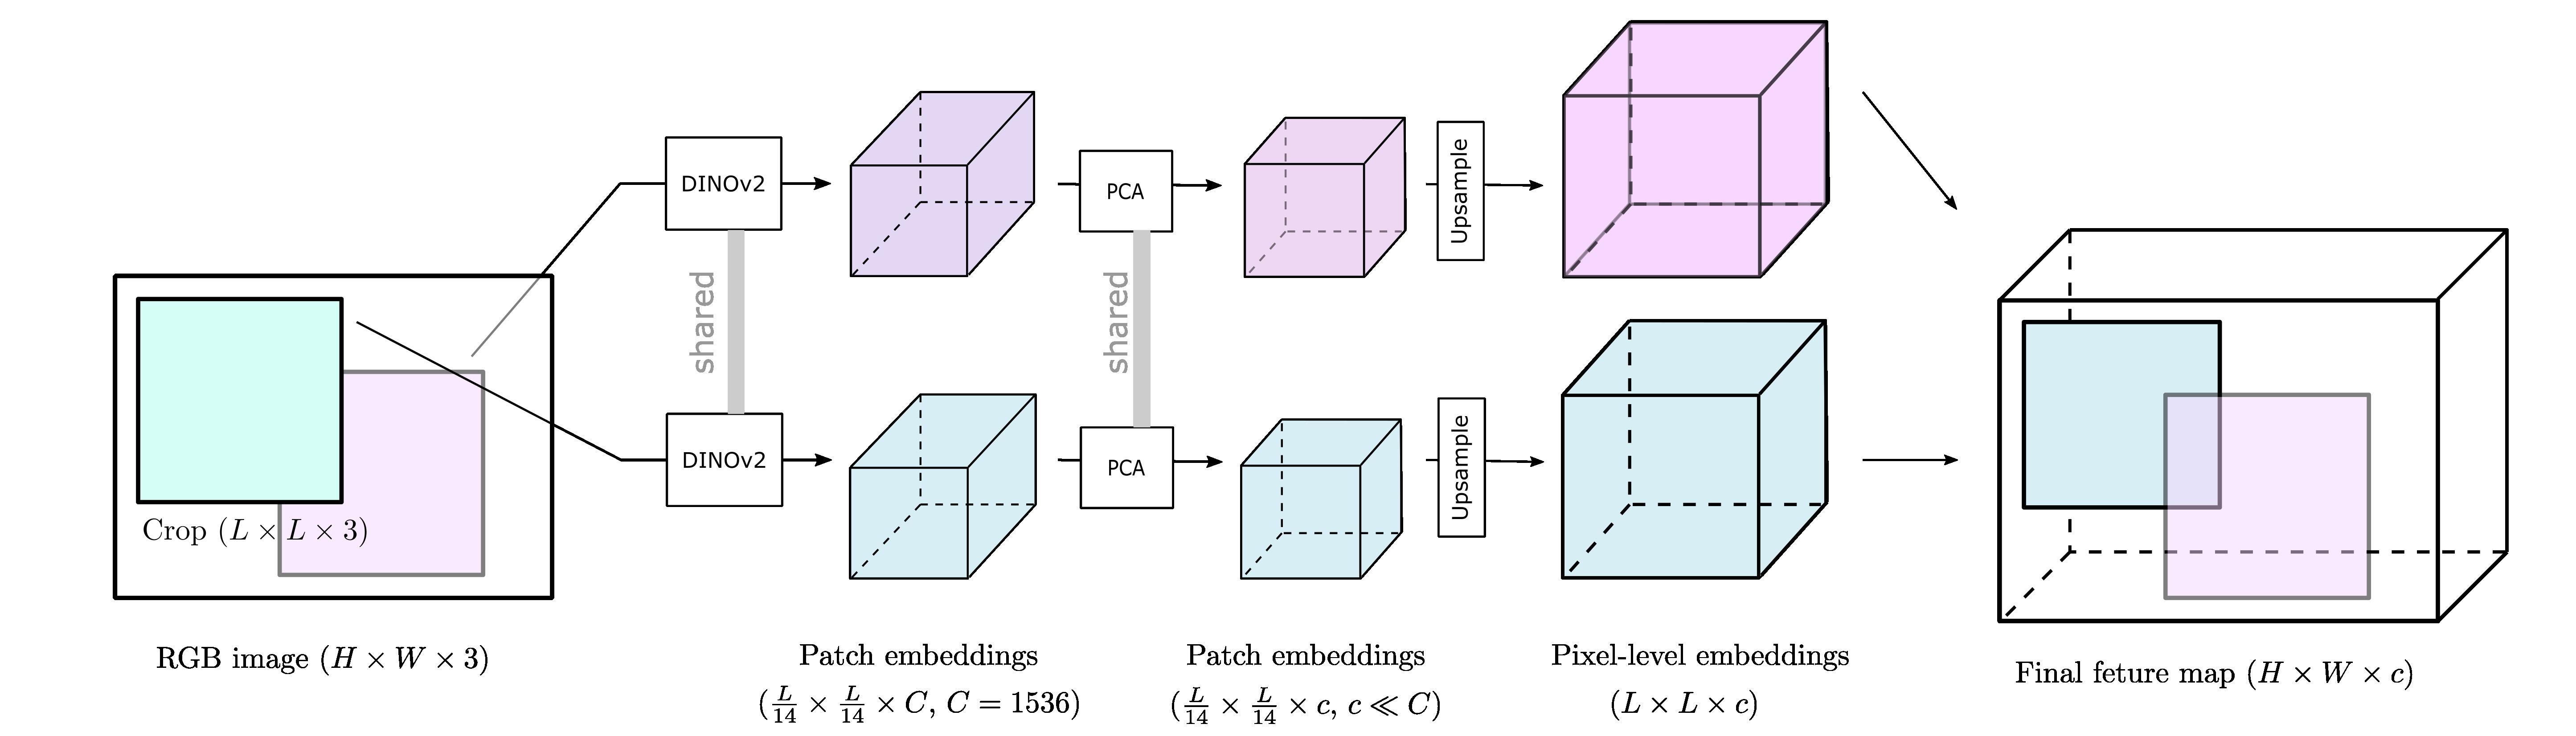
\includegraphics[width=\linewidth]{figures/sliding_windows.jpg}
    \caption{Sliding windows for construction of DINOv2 feature maps.}
    \label{fig:appendix-sliding-windows}
\end{figure*}

\subsection{Enhancing segmentation with DINOv2 using 3D graph diffusion}
\label{sec:appendix-diffusion}

DINOv2 provides generic visual features that do not explicitly include information for segmentation, unlike models such as SAM that were specifically trained for such a task. 
Consequently, using the 2D projections of uplifted DINOv2 features, as proposed in Sec. \ref{sec:appendix-dino_seg}, might fail to separate different objects that happen to have similar features while still being distinct entities. 
This challenge can be mitigated by incorporating 3D spatial information in which the objects are more likely to be well-separated. 
To this end, we propose to leverage the graph diffusion process introduced in Sec.~\ref{sec:diffusion}. 
Below, we describe the initialization of the weight vector $g_0$ and the construction of the adjacency matrix $A$.  

\myparagraph{Initialization of the weight vector} 
The initial vector of weights $g_0\in \mathbb{R}^n$ representing a coarse estimation of the contribution of each Gaussian to the segmentation mask. It is computed by uplifting the 2D \textit{foreground mask} (either scribbles or a reference mask) from the \textit{reference frame} using Eq.~(\ref{eq:uplifting}) from the main paper, and retaining only the top 10\% of Gaussians with positive mask values, setting the rest to zero.
The nodes for which $g_0$ has a positive value define a set of anchor nodes $\mathcal{M}$ that are more likely to contribute to the foreground. The resulting weight vector is a coarse estimation of how much each Gaussian contributes to a rendered 2D segmentation mask.

\myparagraph{Construction of the graph edges}
We define the pairwise similarity function $S_f$ as:
\begin{equation}
    \label{eq:appendix-rbf}
    S_f(f_i, f_j) = \exp\left ( - \frac{||f_i - f_j||_2^2}{b s_f^2} \right)
\end{equation}
 where $f_i, f_j$ are the $l_2$-normalized DINOv2 features, $s_f$ is the median of pairwise $l_2$ distances and $b$ is a bandwidth parameter.
 We choose a global unary regularization term $P(f_i)$ on each node $i$ to contain diffusion to nodes with features similar to those of the foreground. More precisely, $P$ is defined using a similar approach as in Sec.~\ref{sec:appendix-dino_seg}: \begin{enumerate}
     \item When scribblers are provided, $P(f_i) = \mathcal{S}_{f}(f_i, \bar{f})$ with the averaged feature $\bar{f}$ over the anchor nodes $\mathcal{M}$, and a different value for the bandwidth $b$. 
     \item When a full foreground mask is available, we train a logistic regression model on the uplifted features with positive labels for the anchor nodes' features. The unary term is then defined as $P(f_i) = \mathcal{L}(f_i)^{1/b}$, with $b$ a bandwidth parameter and $\mathcal{L}(f_i)$ is the model's predicted probability for $f_i$.
 \end{enumerate}

The local term $S_f$ allows diffusing to neighbors that have similar features while the unary term prevents leakage to background nodes and allows using an arbitrary number of diffusion steps. 

The matrix $A$ of graph edges is then defined based on $S_f$ and $P$ as in Eq.~(\ref{eq:edges}) from the main paper.
For this task, we binarize $A$ with a fixed threshold (set to $10^{-5}$). After the $T$ diffusion steps, we recover the  nodes $\mathcal{S}$ in $g_T$ with strictly positive values (\emph{i.e.}, those reachable after $T$ iterations). The final weight is defined as $h_i = P(f_i)$ if $i\in \mathcal{S}$ and $0$ otherwise. Segmentation is then performed by projecting $\mathbf{h} = (h_i)$ into 2D and thresholding. The selection process of the threshold and bandwidth parameters is detailed below.

\myparagraph{Evaluation and hyperparameter tuning}
Segmentation relies on three hyperparameters: the bandwidths for $S_f$ and $P$, and the threshold for foreground/background pixel assignment. 
For SPIn-NeRF, all hyperparameters are chosen based on the IoU for the available reference mask. For NVOS, only reference scribbles are provided, hence we predict a SAM mask based on the scribbles of the reference frame, and choose the hyperparameters maximizing the IoU with this SAM mask. This is consistent with a scenario where the user, here SAM, would choose hyperparameters based on visual inspection on one of the frames.

\subsection{Open-vocabulary object localization}
\label{sec:appendix-clip}

For the open-vocabulary object localization task, multi-resolution CLIP feature maps are constructed as described in Sec.~\ref{sec:method_clip} 
and uplifted along with DINOv2 features using Eq.~(\ref{eq:uplifting}) from the main paper.
The refined 3D CLIP features are then evaluated on the LERF localization and segmentation tasks as described below.

\subsubsection{Relevancy scores and object localization.}

We consider uplifted 3D CLIP features $f$.
We follow LERF~\citep{kerr2023lerf} and LangSplat~\citep{qin2023langsplat} to compute alignment scores between CLIP visual features and a text query, denoted as \emph{relevancy score}, and for object localization based on these relevancy scores.

\myparagraph{Relevancy scores}
The relevancy $r_{i,q}$ between a feature $f_i$ and text query $\phi_{\text{q}}$ is defined as follows:
\begin{equation}
r_{i,q} = \min_k \frac{\exp(T \cdot f_i \cdot \phi_{q})}{\exp(T \cdot f_i \cdot \phi_{q}) + \exp(T \cdot f_i \cdot \phi_{cano}^k)},
\end{equation}
where $T$ is a temperature parameter set to 10 by~\cite{kerr2023lerf} and $\phi_{\text{cano}}^k$ is the CLIP embedding of a predefined canonical phrase chosen from “object," “things," “stuff," and “texture."
Note that \cite{qin2023langsplat} compute the relevancy scores for 2D pixels, while we directly compute them for 3D Gaussians, allowing their manipulation in 3D.


\myparagraph{Localization}
The 3D CLIP relevancies can be projected into 2D for a given camera pose, and used for localization and segmentation for each text query. For localization, we follow \cite{qin2023langsplat} and choose the pixel with the highest relevancy score, following a 2D smoothing using a mean filter with kernel size $K=5$ in our work. 

\subsubsection{Object segmentation}

Segmentation based on raw CLIP relevancies is challenging, as fully covering the object of interest without capturing other objects of a similar nature is challenging.

We first describe our process for segmenting directly based 3D relevancies. We then present two complementary approaches that allow for a more targeted segmentation: predicting 2D SAM masks by retrieving query points with high relevancies, and refining 3D relevancy scores using graph diffusion based on 3D DINOv2 features.

\myparagraph{Segmentation from 3D relevancies}
Given a camera pose and a text query, a segmentation mask is obtained by first applying a rough thresholding over projected relevancies rescaled by their maximum value, with a fixed threshold value $\tau=0.8$, followed by automatic thresholding with Otsu's method \citep{otsu1975threshold}.

\myparagraph{Improving 2D segmentation with SAM} 
For segmentation with SAM, we use the pixels with the highest relevancy scores as query points for a given camera pose and text query. 
More precisely, we first obtain a mask $\mathcal{M}$ by projecting and thresholding the relevancies as described above, using $\tau=0.93$. We then use the approach described in Sec.~\ref{sec:appendix-sam_seg}, paragraph \emph{Predicting a SAM segmentation mask from a set of query points} and average 20 mask predictions.
We choose the top-$q$ percent of pixels as the subset of query points for SAM, where $q$ is the proportion of positive pixels in $\mathcal{M}$, hence extracting a larger subset of point prompts for larger objects. The scalar map obtained by averaging the 20 predicted masks is then automatically thresholded again using Otsu's method~\citep{otsu1975threshold}.

\myparagraph{Refining 3D CLIP relevancies with graph diffusion based on DINOv2 features}
We refine 3D CLIP relevancy scores using graph diffusion based on 3D DINOv2 features ($f$), as in Sec.~\ref{sec:appendix-diffusion}. The diffusion process runs in parallel for all text queries. For initialization, we keep positive a very restricted set of nodes with the highest relevancy, whose weight propagate to neighboring nodes with similar DINOv2 features, progressively spanning the object of interest. The diffusion process results in a better segmentation both with and without leveraging SAM. When using SAM, the set of query pixels can have a larger coverage of the object of interest without extending to other objects.

\myparagraph{Details on graph construction and node initialization for refining 3D CLIP relevancies}
The pairwise similarity function $S_f$ is defined as in Eq.~\ref{eq:appendix-rbf} with a bandwidth value $b=0.5$. For each text query $\phi_q$, we define a unary regularization term $P_q$ using a logistic regression model $\mathcal{L}_q$ that predicts the probability that a DINOv2 feature $f_i$ belongs to the object corresponding to query $\phi_q$. The set of nodes $\mathcal{P}$ with positive labels is defined based on 3D CLIP relevancy scores for prompt $\phi_q$. More precisely, we rescale 3D relevancies to $[0,1]$ and apply Otsu's method~\citep{otsu1975threshold} over relevancies above $0.5$. We use a regularization $C=0.001$ and equal class weighting for training the model.
The unary regularization term $P_q$ is then defined as $P_q(f_i) = \mathcal{L}_q(f_i)^{1/b}$, with $b=0.025$ for segmentation with SAM, and $b=2$ otherwise.
The initial weight vector $g_0$ is defined by applying two more iterations of Otsu's method among nodes in $\mathcal{P}$ and setting to zero all relevancies below the given threshold. Restricting the set of initial points ensures diffusion only happens within the object of interest. Segmentation based on the resulting 3D relevancy scores is then performed as described in the previous paragraphs, using $\tau=0.01$ for segmentation with SAM and $\tau=0$ otherwise. 

\begin{table*}[t!]
\centering
\footnotesize
\scalebox{1.}{
\begin{tabular}{lccccccccccccc}
\toprule
& \multicolumn{2}{c}{\textbf{Images (\#)}} &  \multicolumn{2}{c}{\textbf{Text queries (\#)}} & \multicolumn{2}{c}{\textbf{DINOv2 (s)}} & \textbf{CLIP (s)} & \multicolumn{2}{c}{\textbf{Graph diffusion (s)}} & \multicolumn{2}{c}{\textbf{2D segmentation (s)}} & Total \\
\cmidrule(lr){2-3} \cmidrule(lr){4-5} \cmidrule(lr){6-7} \cmidrule(lr){8-8} \cmidrule(lr){9-10} \cmidrule(lr){11-12}
Scene & Train & Test & Unique & Total & Gen. & Up. & Gen.+Up. &  Scene & Prompt & w/ SAM & w/o SAM & (mins) \\
\midrule
Teatime   & 177 & 6 & 14 & 59  & 45 & 14 & 363 & 42 & 15 & 9 & 0.9 & 8 \\
Waldo     & 187 & 5 & 18 & 22  & 44 & 18 & 371 & 39 & 19 & 4 & 0.5 & 8 \\
Ramen     & 131 & 7 & 14 & 71 & 40 & 9 & 227 & 37 & 14 & 11 & 1 & 6  \\
Figurines & 299 & 4 & 21 & 56  & 58 & 38 & 811 & 45 & 22  & 8 & 0.8 & 16  \\
\bottomrule
\end{tabular}
}
\caption{\textbf{Runtimes for evaluation on LERF Segmentation~\citep{kerr2023lerf, qin2023langsplat}.} 
The last column (Total) reports total time, which breaks down between i) feature map generation (Gen.) and uplifting (Up.) for all training images; ii) graph diffusion, divided between scene-specific (querying neighbors, defining $S_f$) and prompt-specific (defining $P$, running diffusion) operations for all text queries; iii) 2D segmentation with/without SAM for all text queries across test images. We also report the number of training and test images and the number of text queries across test images.}
\label{tab:runtimes}
\end{table*}
\begin{table*}[t!]
\centering
\footnotesize

\begin{subtable}{\linewidth}
\centering
\scalebox{.99}{
\begin{tabular}{lcccccc}
\toprule
 & \multirow{2}{*}{SA-TensoRF} & \multirow{2}{*}{SA-GS} & \multirow{2}{*}{OmniSeg3D} & \multirow{2}{*}{SAGA} & \multicolumn{2}{c}{LUDVIG} \\
%\cmidrule(lr){6-7}
 & & & & & SAM & DINOv2 \\
\midrule
2D feature extraction (sec.) & 30 & 30 & 900\footnotemark & 900$\footnotemark[1]$ & 20 & 30 \\
3D feature training (sec.) & \emph{15} & \emph{4} & 900 & 1500 & \emph{4} & 40+\emph{2} \\
%Inference & 15s  & 4s & 50--100 ms & 2--5 ms & 4s & $2s$  \\
%Inference (s) & 15  & 4 & 3 & 0.2-0.4 & 4 & 2  \\
\bottomrule
\end{tabular}
}
\caption{\textbf{Multi-view segmentation (NVOS)}. \emph{Italic} denote inference-time operations (after 2D scribbles are given). OmniSeg3D and SAGA avoid inference overhead but require longer feature extraction and training\vspace{.1cm}.}
\end{subtable}
\begin{subtable}{\linewidth}
\centering
\scalebox{.99}{
\begin{tabular}{lcccccc}
\toprule
 & \multirow{2}{*}{LERF} & \multirow{2}{*}{LangSplat} & \multirow{2}{*}{OpenGaussian} & \multicolumn{2}{c}{LUDVIG} \\
%\cmidrule(lr){5-6}
& & & & w/o diff. & w/ diff. \\
\midrule
2D feature extraction (min) & - & ~$50$\footnotemark[1] & ~$50$\footnotemark[1] & 4.5 & 4.5 \\
3D feature training (min) & 25 & 25 & 40 & 2 & 2.5 \\
Inference (s/query) & 30.9 & 0.26 & $\sim0.2$~~~ & 0.3 & 1.3 \\
\bottomrule
\end{tabular}
}
\caption{\textbf{Open-vocabulary segmentation (Ramen scene) \vspace{-.2cm}.} 
}
\end{subtable}
\vspace{-.15cm}
\caption{\textbf{Training and inference times.} All methods build on top of a GS pretraining stage ($\sim 10$min). Reported values are paper-sourced and indicative, as hardware setups may differ.
}
\vspace{-.2cm}
\label{tab:rebuttal-times}
\end{table*}



\section{Runtime analysis}

\subsection{Runtimes for LUDVIG}
\label{sec:appendix-runtime}

In this section, we detail our running times for feature uplifting and evaluation, conducted on a GPU RTX 6000 ADA. Table~\ref{tab:runtimes} shows a breakdown of running times between feature uplifting (Up.) and generation (Gen.), graph diffusion and 2D segmentation for evaluation on LERF segmentation. 
The total reported times can be divided between pre-uplifting, uplifting and post-uplifting. In our experiments, the pre-processing and uplifting steps are independent from the downstream tasks (except for our foreground/background segmentation with SAM), and part of the graph-diffusion process is task-dependent. Below we detail our runtimes for every step and compare them to the literature.

\myparagraph{Pre-uplifting: feature map generation} The time this step takes (Gen. in Table~\ref{tab:runtimes}) depends on the backbone model, on the number of images and on the number of calls to the model per image. The total time ranges from a few seconds up to an hour for approaches such as LangSplat \citep{qin2023langsplat}, that queries SAM over a grid of points on the image at various resolutions to generate full image segmentation masks.\footnote{This process takes 24s/image on a GPU 6000 ADA and amounts to an average of 80 minutes for the evaluated scenes.} In our experiments, the feature generation step takes from 1 to 5 minutes, except for Sec.~\ref{sec:exp-semantic} where we uplift semantic maps generated with LangSplat's approach.

\myparagraph{Uplifting} For LUDVIG, uplifting time is linear in the number of images (given a 3D scene representation). Experimentally, it is also linear in the number of feature dimensions, taking 2ms per dimension for an image of size $724 \times 986$. As reported in Table~\ref{tab:runtimes} (Up.), uplifting 100 images of dimension $40$ takes 9s on average. By contrast, gradient-based optimization requires approximately $n_{\text{steps}}$ times this duration, where the number of gradient steps $n_{\text{steps}}$ typically ranges from 3,000 to 30,000 for 3D feature distillation~\citep{kerr2023lerf, qin2023langsplat, zuo2024fmgs}. Gradient-based optimization can still be very fast for low-dimensional features such as SAM masks (can take as little as a few seconds, as reported by SA3D-GS~\citep{cen2023segmentGS}) or dimensionality-reduced features (LangSplat~\citep{qin2023langsplat} trains an autoencoder to reduce the CLIP feature dimension from 512 to 3 and runs for 25 minutes). However, optimization becomes intractable for high-dimensional features such as CLIP and DINO; FMGS~\citep{zuo2024fmgs} relies on an efficient multi-resolution hash embedding of the scene; however, their total training time still amounts to 1.4 hours.

\myparagraph{Post-uplifting: graph diffusion} After uplifting, LUDVIG performs graph diffusion using pairwise DINOv2 feature similarities for the segmentation tasks in Sec.~\ref{sec:exp-seg} and \ref{sec:exp-clip}. In Table~\ref{tab:runtimes}, we divide runtimes in two categories: 
\begin{itemize}
    \item \textbf{Scene}: operations performed once for the whole scene. This includes querying the Euclidean neighbors for each node, which is log-linear in the number of Gaussians. With 600,000 Gaussians as in our experiments, the step takes about 30s, and can be further optimized by using approximate nearest neighbor search algorithms~\citep{wang2021comprehensive}. Defining $S_f$ based on DINOv2 features is also independent from the downstream task.
    \item \textbf{Prompt}: operations that are specific to the downstream task. This includes defining the regularization $P$ (\emph{e.g.} training logistic regression model(s)) and running the diffusion. The time taken depends on dimension of the diffused features (\emph{e.g.} number of text queries): 1 to 2 seconds for foreground/background segmentation (a single mask) and 18 seconds on average for LERF segmentation (14 to 21 text queries).
\end{itemize}

\myparagraph{Post-uplifting: segmentation} Our evaluation on LERF involves 2D segmentation with SAM based on 3D relevancy scores. The runtime depends on the number of test images and on the total number of 2D text queries, as it involves one call to the SAM backbone per test image, and multiple calls to the SAM prediction head per text query, as detailed in Appendix~\ref{sec:appendix-clip}. Our total inference time per scene is of $8 s$ on average, against $0.8 s$ when not using SAM. In contrast, Langsplat does not rely on SAM at inference time, but relies on a computationally expensive feature map generation process, with more than 1 hour runtime. 


\subsection{Runtime comparisons}
\label{sec:appendix-runtime-comp}

Table~\ref{tab:rebuttal-times} reports runtime comparisons for the multi-view~(Sec.~\ref{sec:exp-seg}) and open-vocabulary (Sec.~\ref{sec:exp-clip}) segmentation tasks.
%
Compared to approaches relying on SAM's automatic mask generation, such as OmniSeg3D~\citep{ying2023omniseg3d}, SAGA~\citep{cen2023saga}, LangSplat~\citep{qin2023langsplat}, and OpenGaussian~\citep{wu2024opengaussian}, our method offers significantly faster feature generation and uplifting, at the cost of a slightly higher inference time.
In particular, the graph diffusion step adds approximately 1~second per query at inference (reported as 14~seconds for Ramen’s 14 queries in supplementary Table~\ref{tab:runtimes}).

Our experiments in Sec.~\ref{sec:exp-semantic} show that our uplifting process can serve as a drop-in replacement for the training phase in methods optimized for fast inference, such as OpenGaussian~\citep{wu2024opengaussian}, which learns from 2D feature maps generated using LangSplat’s approach. In these experiments, we adopt the same 2D feature map generation and evaluation protocols as OpenGaussian, replacing only their quantization-based training phase with our fast feature aggregation. This results in significantly faster uplifting while achieving notable accuracy gains.

\begin{table*}[t!]
  \centering
  \footnotesize
\begin{tabular}{lccccccc}
\toprule
& \multirow{1}{*}{MVSeg} & \multirow{1}{*}{SA3D-GS} & \multirow{1}{*}{SAGA} & \multirow{1}{*}{OmniSeg3D} & \multicolumn{3}{c}{LUDVIG (Ours)}  \\
\cmidrule(lr){6-8}
3D representation: & NeRF & GS & GS & NeRF &  \multicolumn{3}{c}{GS} \\
Uplifting: &  & SAM & SAM & SAM & DINOv2 & SAM & SAM2 \\
\midrule
Orchids      & 92.7 & 84.7 & - & 92.3 & 92.6 & 92.2 & 91.0 \\
Leaves  & 94.9 & 97.2  & - & 96.0  & 96.2 & 96.3 & 96.3 \\
Fern & 94.3 & 96.7 & - & 97.5 & 96.3 & 97.0 & 97.0 \\
Room   & 95.6 & 93.7 & - & 97.9 & 95.7 & 96.5 & 96.1 \\
Horns  & 92.8 & 95.3 & - & 91.5 & 95.1 & 94.5 & 94.8 \\
Fortress   & 97.7 & 98.1 & - & 97.9  & 97.5 & 98.3 & 98.3 \\
\midrule
Fork   & 87.9 & 87.9 & - & 90.4 & 85.0 & 86.8 & 86.7 \\
Pinecone   & 93.4 & 91.6 & - & 92.1 & 93.2 & 88.8 & 90.7  \\
Truck   & 85.2 & 94.8 & - & 96.1 & 95.6 & 94.9 & 93.9 \\
Lego   & 74.9 & 92.0 & - & 90.8 & 91.1 & 92.7 & 92.9 \\
\midrule
Average  & 90.9 &  93.2  & 93.4 & 94.3 & 93.8 & 93.8 & 93.8 \\
\hline
\end{tabular}
  \caption{Segmentation (IoU) on SPIn-NeRF~\citep{mirzaei2023spin} with DINOv2, SAM and SAM2.}
  \label{tab:spin}
\end{table*}
\begin{table*}[t!]
  \centering
  \footnotesize
\begin{tabular}{lccccccccc}
\toprule
& Fern & Flower & Fortress & HornsC & HornsL & Leaves & Orchids & Trex & Average \\
\midrule
NVOS & - & - & - & - & - & - & - & - & 70.1  \\
SA3D & 82.9 & 94.6 & 98.3 & 96.2 & 90.2 & 93.2 & 85.5 & 82.0 & 90.3  \\
OmniSeg3D & 82.7 & 95.3 & 98.5 & 97.7 & 95.6 & 92.7 & 84.0 & 87.4 & 91.7  \\
SA3D-GS & - & - & - & - & - & - & - & - & 92.2  \\
SAGA & - & - & - & - & - & - & - & - & 92.6  \\
Ours-DINOv2 & 84.5 & 95.6 & 97.5 & 97.3 & 93.4 &  96.3 & 91.7 & 84.7 & 92.4    \\
Ours-SAM & 85.5 & 97.6 & 98.1 & 97.9 & 94.1 & 96.4 & 73.1 & 88.0  & 91.3    \\
Ours-SAM2 & 84.8 & 97.3 & 98.3 & 97.7 & 93.4 & 96.7 & 73.1 & 89.1 & 91.3    \\
\hline
\end{tabular}
  \caption{Segmentation (IoU) on NVOS~\citep{ren2022nvos} with DINOv2, SAM and SAM2.}
  \label{tab:nvos}
\end{table*}
\begin{table*}[t!] 
\centering \footnotesize 
\begin{tabular}{lcccccc} 
\toprule
& Geometry only & \multicolumn{2}{c}{Single view} & \multicolumn{2}{c}{Uplifting} & \multicolumn{1}{c}{Graph diffusion} \\
\cmidrule(lr){3-4} \cmidrule(lr){5-7}
Model: & Reference mask & DINOv2 & SAM2 & DINOv2 & SAM2 & DINOv2 \\ 
\midrule 
Orchids & 71.3 & 91.5 & 78.4 & 91.5 & 91.0 & 92.6 \\ 
Leaves &  72.4 & 89.3 & 96.6 & 94.1 & 96.3 & 96.2 \\ 
Fern &  93.9 & 95.1 & 96.7 & 96.7 & 97.0 & 96.3 \\ 
Room &  77.4 & 95.4 & 95.6 & 97.3 & 96.1 & 95.7 \\ 
Horns &  80.7 & 90.9 & 93.0 & 94.2 & 94.8 & 95.1 \\ 
Fortress &  94.3 & 96.8 & 97.7 & 98.6 & 98.3 & 97.5 \\ 
\midrule 
Fork &  67.5 & 85.6 & 80.5 & 88.8 &  86.7 & 85.0 \\ 
Pinecone &  56.5 & 92.8 & 67.8 & 89.6 & 90.7 & 93.2 \\ 
Truck &  60.1 & 83.6 & 90.9 & 95.2 & 93.9 & 95.6 \\ 
Lego &  57.3 & 64.4 & 89.0 & 69.9 & 92.9 & 91.1 \\
\midrule 
Average & 73.1 & 88.5 & 88.6 & 91.6 & 93.8 & 93.8 \\
\bottomrule 
\end{tabular} 
\caption{\textbf{Segmentation (IoU) on SPIn-NeRF~\citep{mirzaei2023spin}}. We compare purely geometrical reference mask uplifting and reprojection, single-view prediction, feature/mask uplifting, and graph diffusion leveraging DINOv2 or SAM2.} \label{tab:ablation-spin-dino-sam}
\end{table*}

\section{Additional results}

\subsection{Per-scene multi-view segmentation results}
\label{sec:appendix-seg_scene}

In this section, we present per-scene segmentation results on NVOS and SPIn-NeRF in Tables~\ref{tab:spin},~\ref{tab:nvos} and \ref{tab:ablation-spin-dino-sam}, along with an extended analysis of these results.

\myparagraph{Segmentation on SPIn-NeRF}
We report our segmentation results for the SPin-NeRF dataset~\citep{mirzaei2023spin} in Table~\ref{tab:spin}.
Our results are comparable to the state of the art while not relying on optimization-based approaches. Surprisingly, our segmentation with DINOv2 using graph diffusion also gives results on par with models leveraging SAM masks. 
Our lower segmentation results compared to OmniSeg's can be partly attributed to poor Gaussian Splatting reconstruction of highly specular scenes such as the Fork, in which semi-transparent Gaussians floating over the object try to represent reflections or surface effects that are difficult to capture with standard rasterization techniques~\citep{jiang2024gaussianshader}.

\myparagraph{Segmentation on NVOS}
We report our segmentation results for the NVOS dataset~\citep{ren2022nvos} in Table~\ref{tab:nvos}. 
Our results are comparable to those obtained by prior work. Again, DINOv2 performs surprisingly well while not having been trained on billions of labeled images like SAM. Compared to SAM, DINOv2 better captures complex objects, but sometimes also captures some background noise. This can be seen in Appendix Fig.~\ref{fig:appendix-nvos} with the example of Trex: while SAM misses out the end of the tail as well as the end of the ribs, DINOv2 captures the whole Trex, but also captures part of the stairs behind. Visualisations of Orchids in Appendix Fig.~\ref{fig:appendix-nvos} also explain the lower performance of SAM on this scene: the two orchids SAM is missing are not covered by the positive scribbles, which makes the task ambiguous.

\myparagraph{Ablation study}
In Table \ref{tab:ablation-spin-dino-sam}, we compare our segmentation protocol using DINOv2 and SAM2 to multiple simpler variants. More precisely, we evaluate i) a purely geometrical variant that does not use SAM2 or DINOv2, ii) single-view segmentation in 2D based on SAM2 or DINOv2 2D predictions, iii) uplifting DINOv2 features or SAM2 masks into 3D then rendering them for segmentation, as described in Sec.~\ref{sec:appendix-sam_seg} and \ref{sec:appendix-dino_seg}, and iv) segmenting using graph diffusion over DINOv2 3D feature similarities.

The purely geometrical approach works well on the forward-facing LLFF scenes (Orchids to Fortress). In these scenes, the reference mask is accurately uplifted and reprojected as the viewing direction changes only a little between each frame. However, it fails on the 360-degree scenes (Fork, Pinecone, Truck, Lego). This points to a suboptimal 3D reconstruction of the scene, likely due to overfitting on the limited numbers of available views~\citep{chung2024depth}.

The single-view variants use a similar process for constructing the features and using them for segmentation as in Sec.~\ref{sec:appendix-sam_seg} and \ref{sec:appendix-dino_seg} but without uplifting and rendering. It improves from a purely geometrical approach and performs reasonably well on average, the foreground being well isolated from the rest of the scene. However, as illustrated in Fig.~3, %\ref{fig:pca}, 
the semantic features are at a much lower resolution than those resulting from 3D uplifting, leading to a coarser segmentation.

3D uplifting considerably boosts results compared to single-view approaches. However, performing segmentation in 2D based on the uplifted DINOv2 features does not benefit from the 3D spatial information and typically fails on the 360-degree scenes (Pinecone, Truck and Lego) which have higher variability across different views. Introducing 3D spatial information through 3D graph diffusion results in a boosted performance on these scenes.

\section{Additional visualizations}

\subsection{Segmentation tasks}

\myparagraph{Segmentation on NVOS}
Fig.~\ref{fig:appendix-nvos} shows our segmentation masks from SAM and DINOv2 for the three most challenging scenes of the NVOS dataset: Fern, Orchids and Trex.

\begin{figure*}[t!]
    \centering
    \begin{subfigure}{.24\linewidth}
        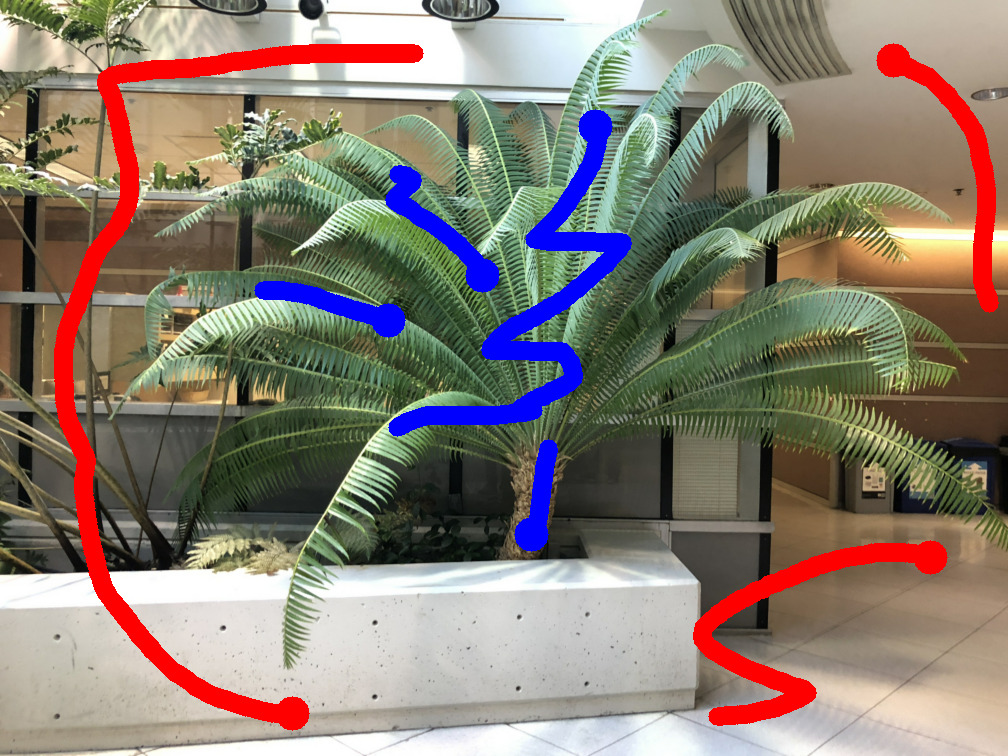
\includegraphics[width=\linewidth]{figures/nvos/fern_reference.jpg}
        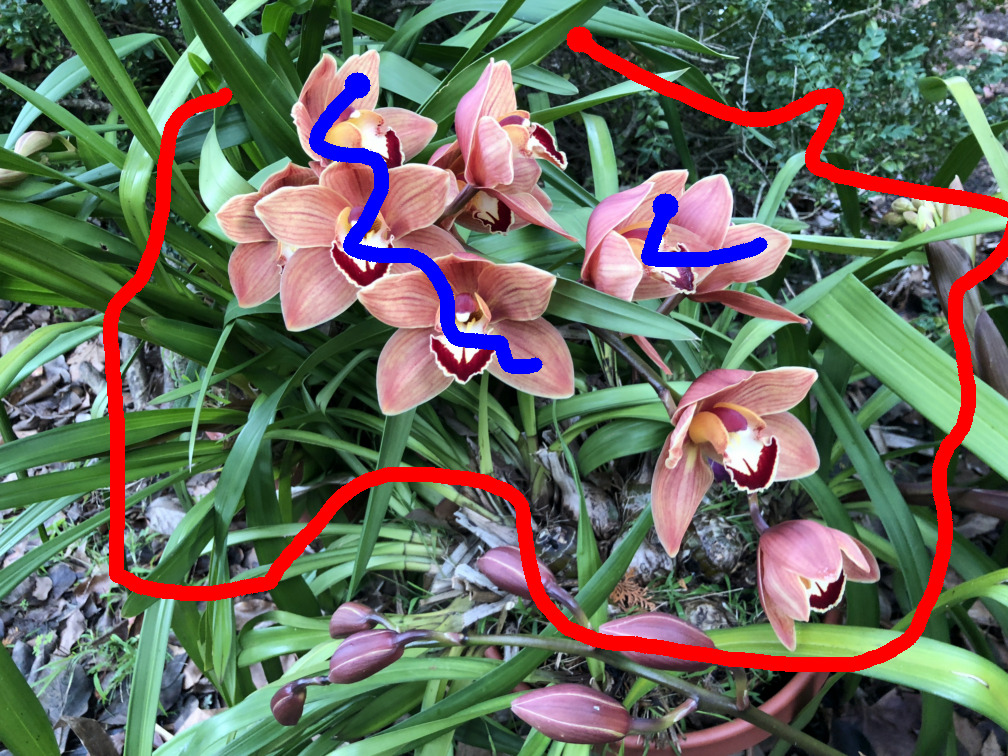
\includegraphics[width=\linewidth]{figures/nvos/orchids_reference.jpg}
        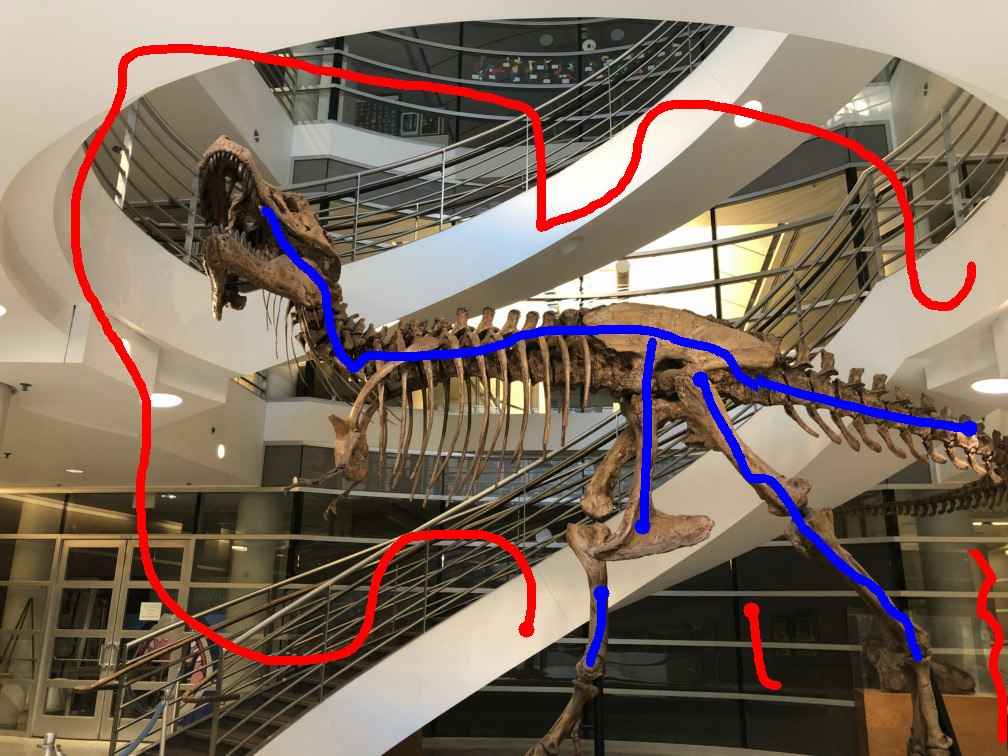
\includegraphics[width=\linewidth]{figures/nvos/trex_reference.jpg}
        \caption{Reference image}
    \end{subfigure}
    \begin{subfigure}{.24\linewidth}
        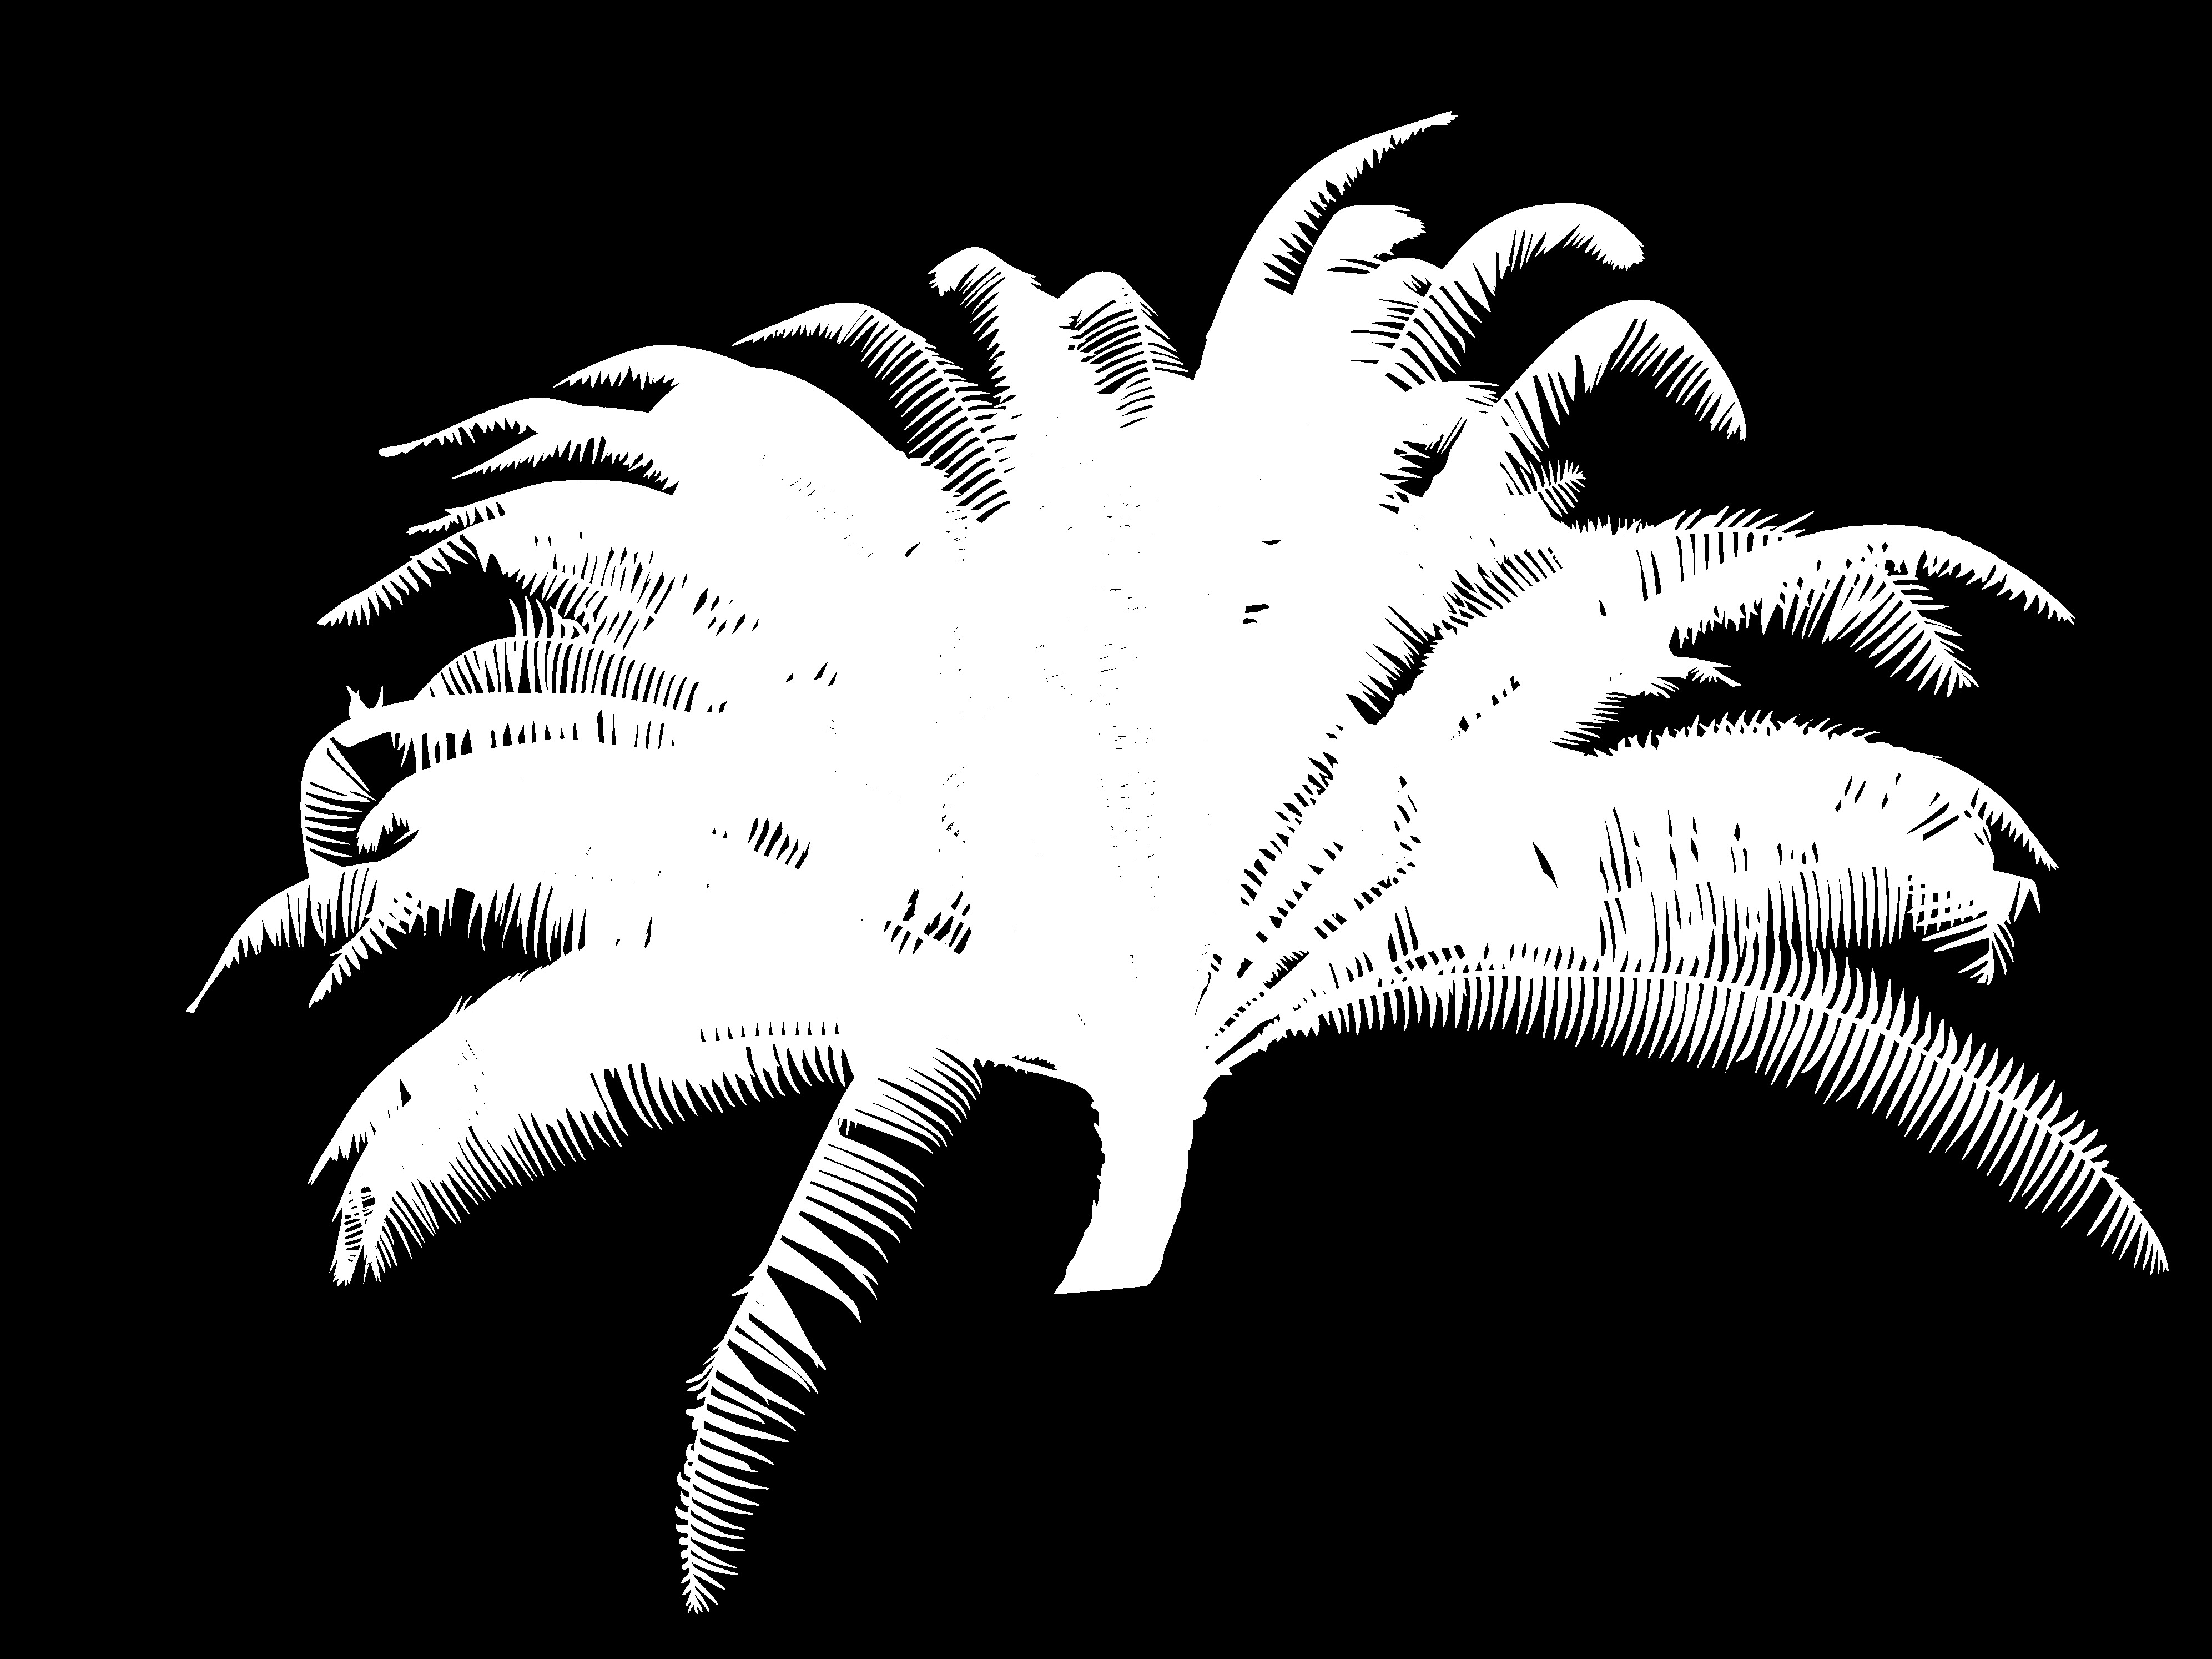
\includegraphics[width=\linewidth]{figures/nvos/fern_mask.jpg}
        
\includegraphics[width=\linewidth]{figures/nvos/orchids_mask.JPG}
        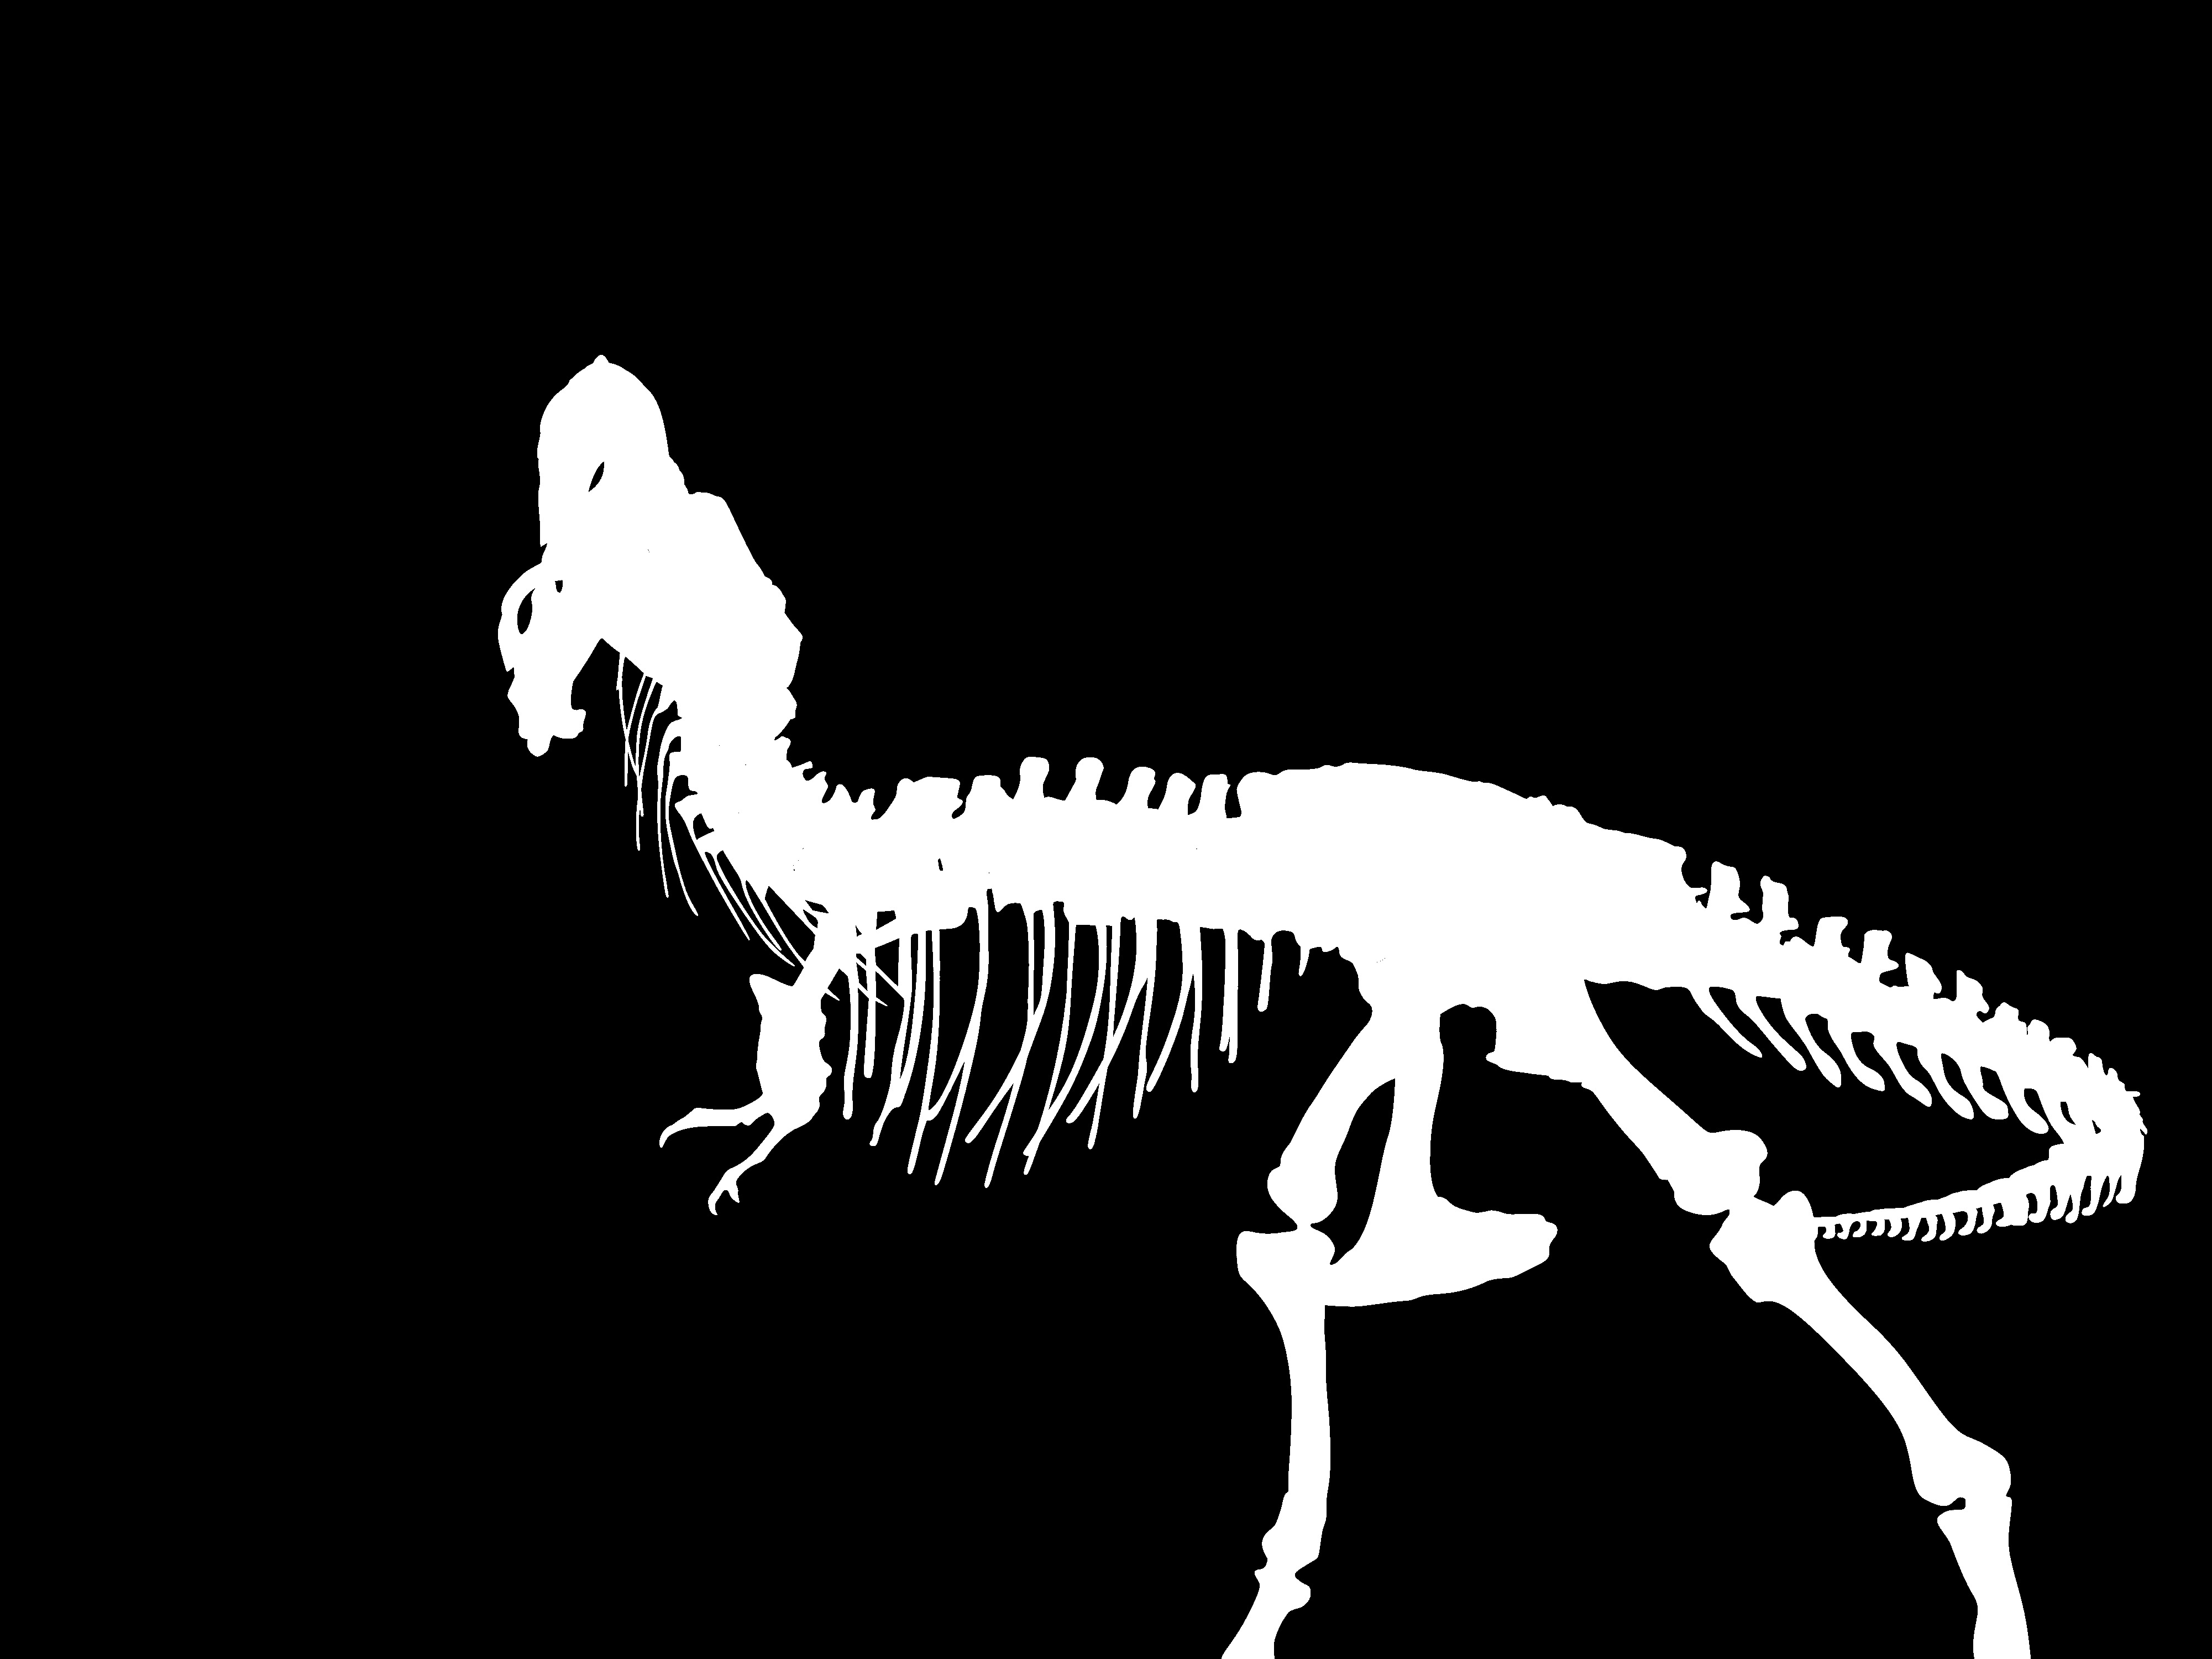
\includegraphics[width=\linewidth]{figures/nvos/trex_mask.jpg}
        \caption{Ground truth mask}
    \end{subfigure}
    \begin{subfigure}{.24\linewidth}
        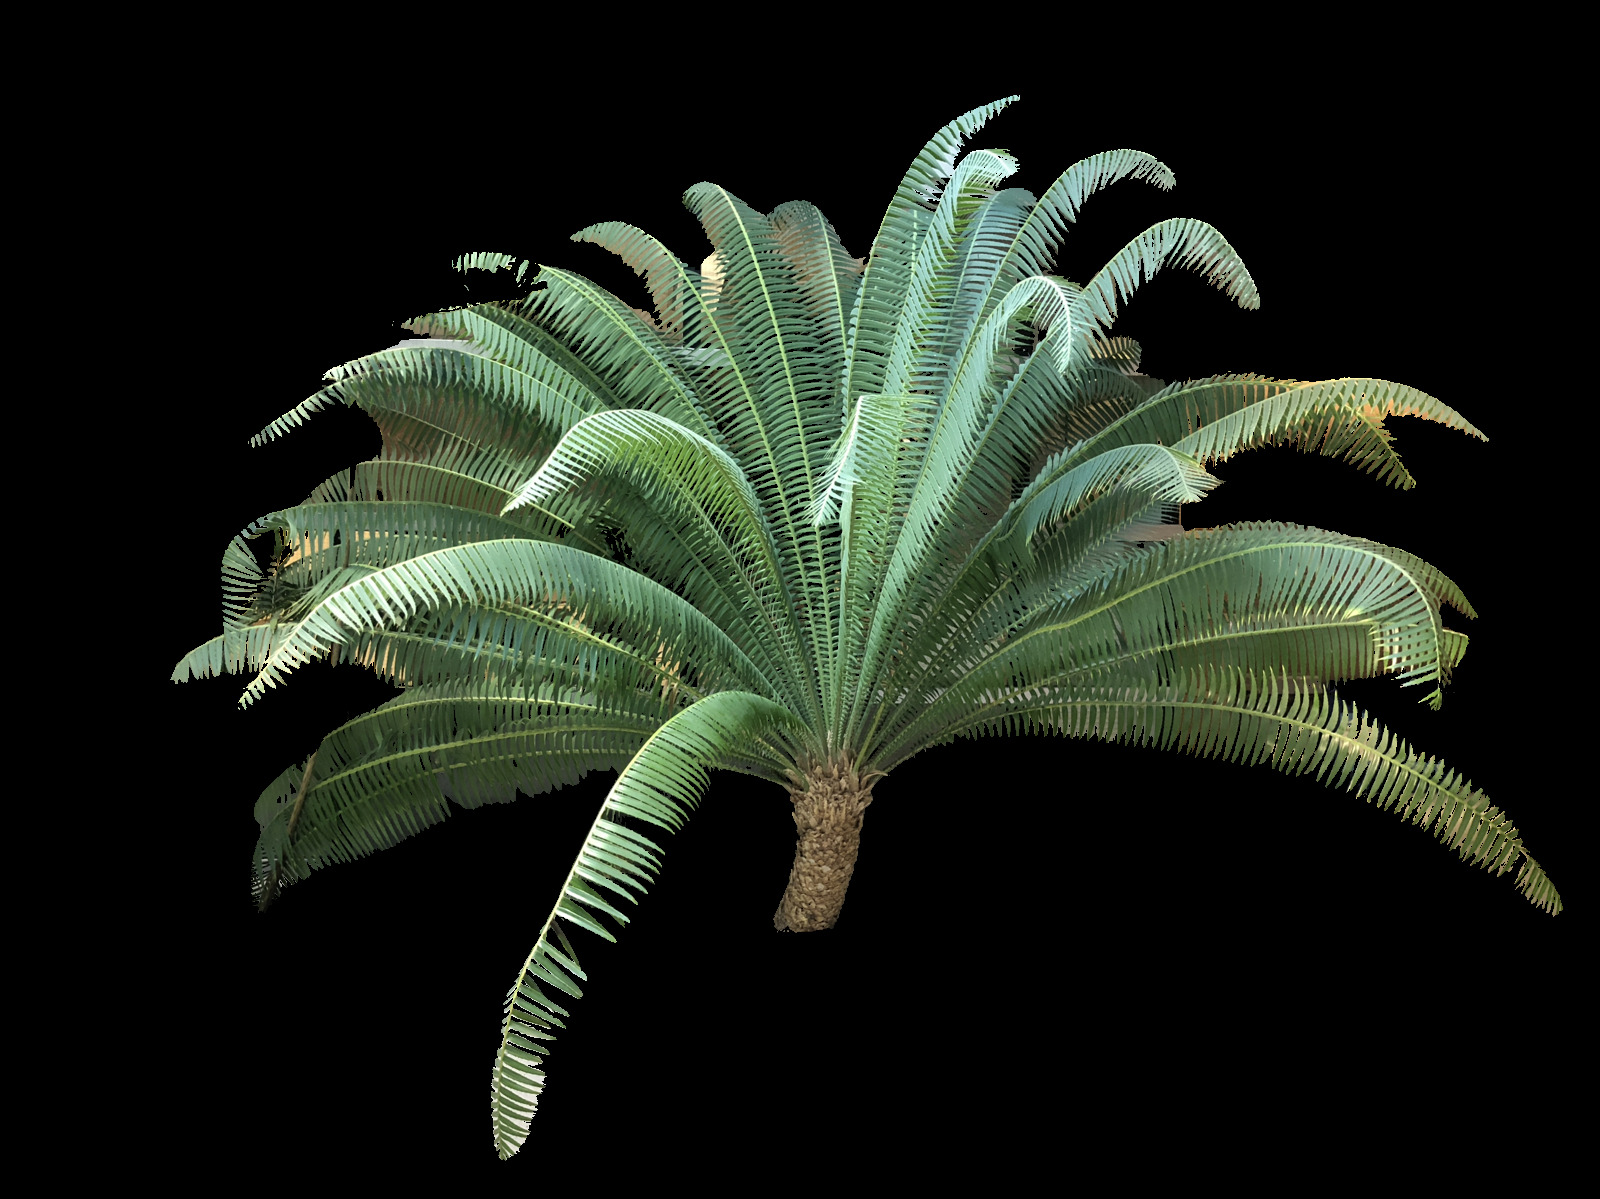
\includegraphics[width=\linewidth]{figures/nvos/fern_sam.jpg}
        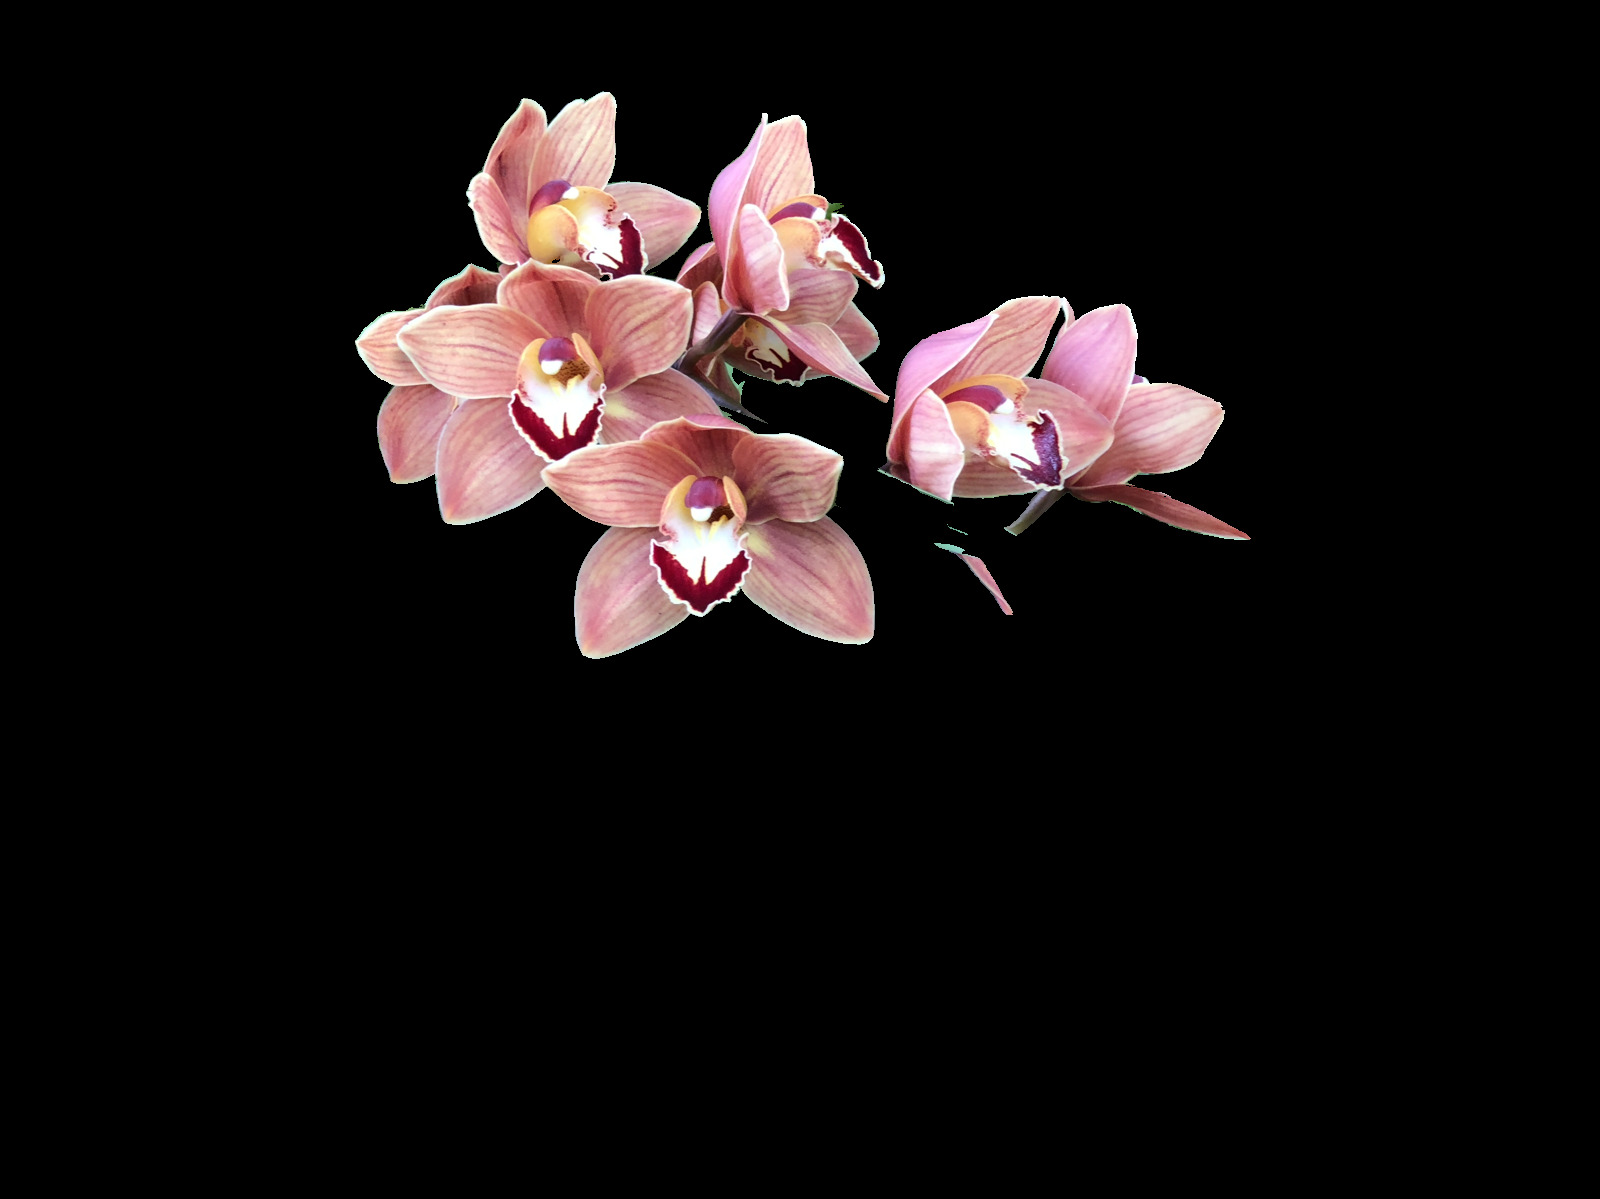
\includegraphics[width=\linewidth]{figures/nvos/orchids_sam.jpg}
        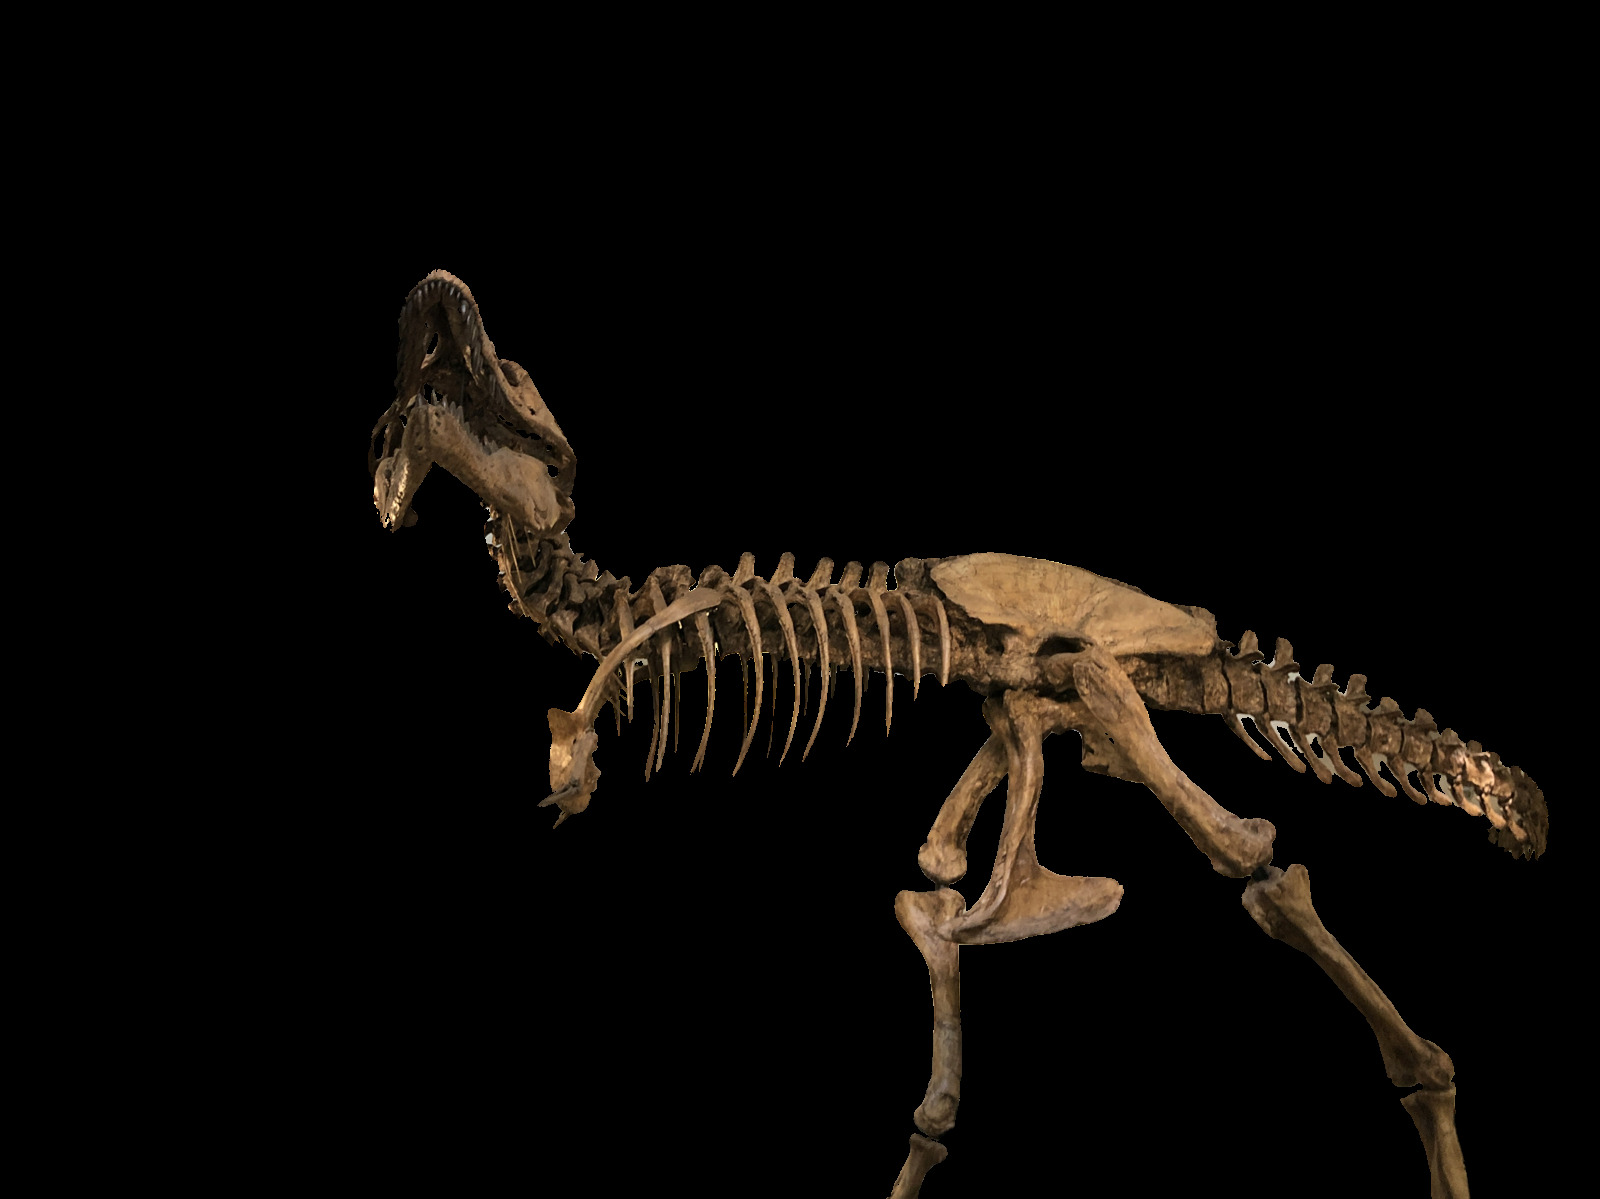
\includegraphics[width=\linewidth]{figures/nvos/trex_sam.jpg}
        \caption{DINOv2 mask}
    \end{subfigure}
    \begin{subfigure}{.24\linewidth}
        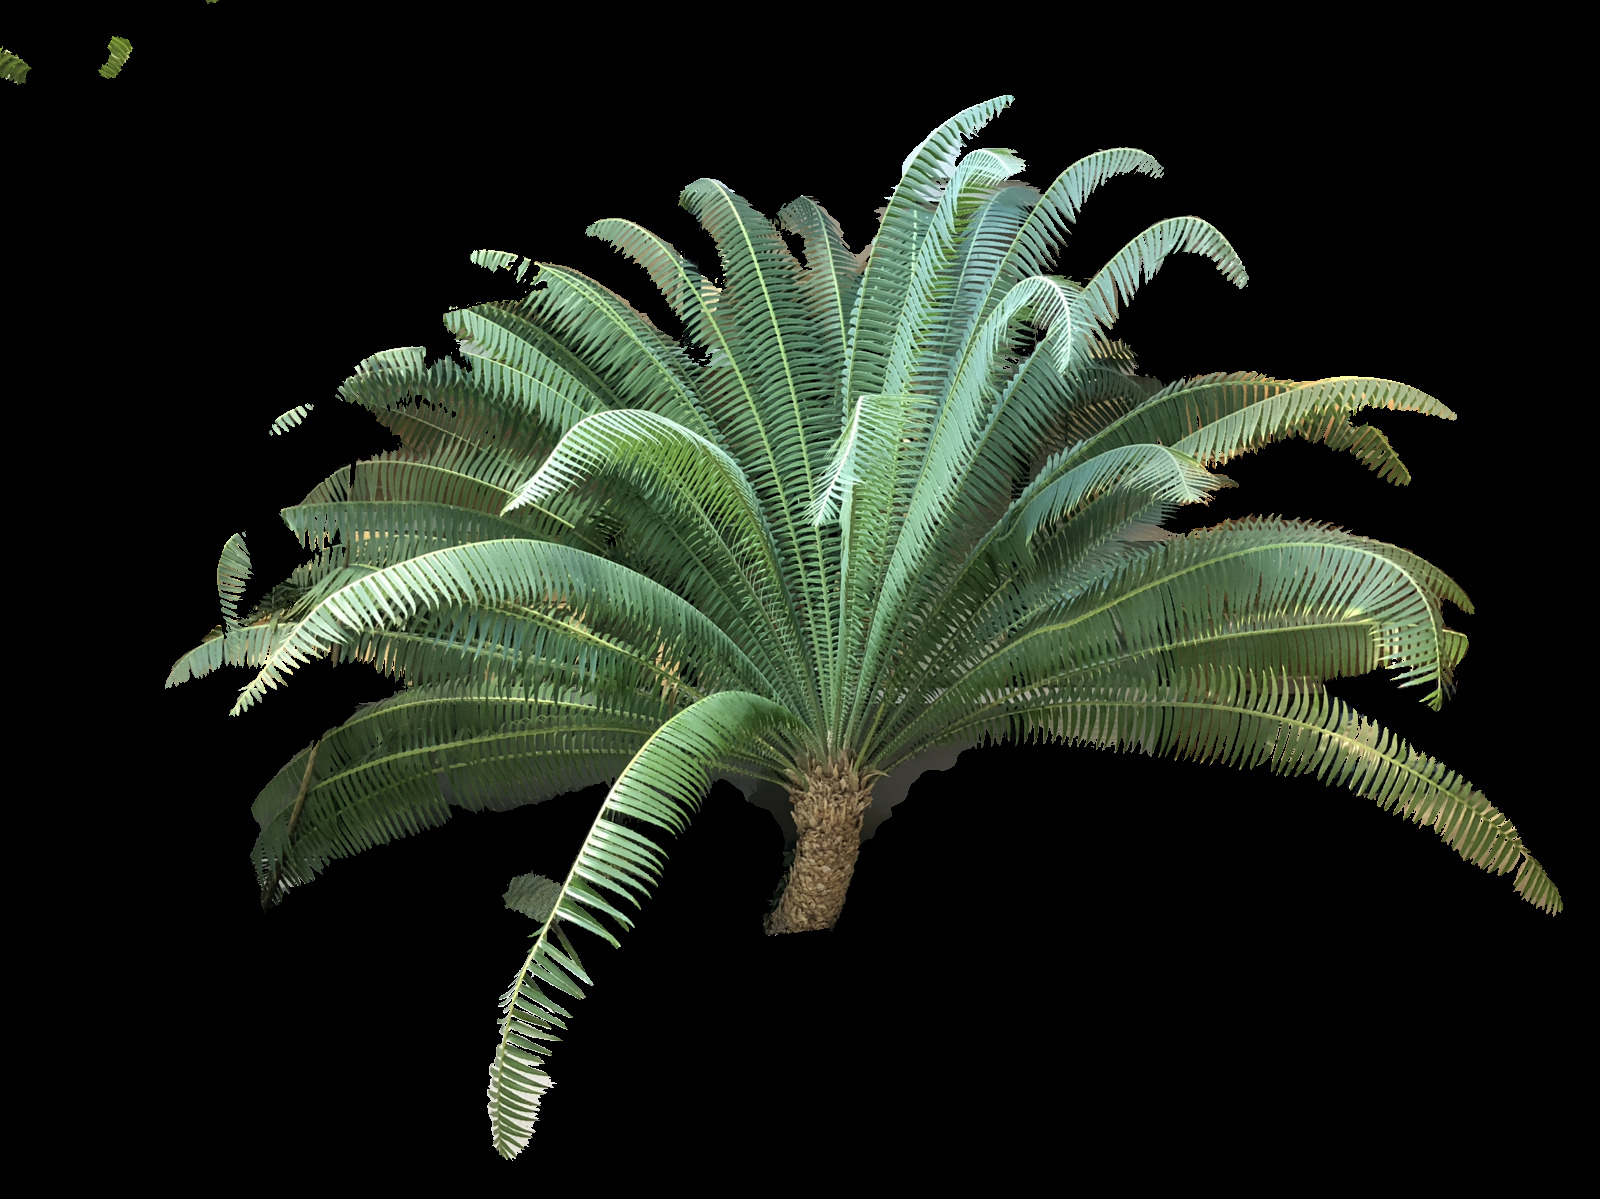
\includegraphics[width=\linewidth]{figures/nvos/fern_dinov2.jpg}
        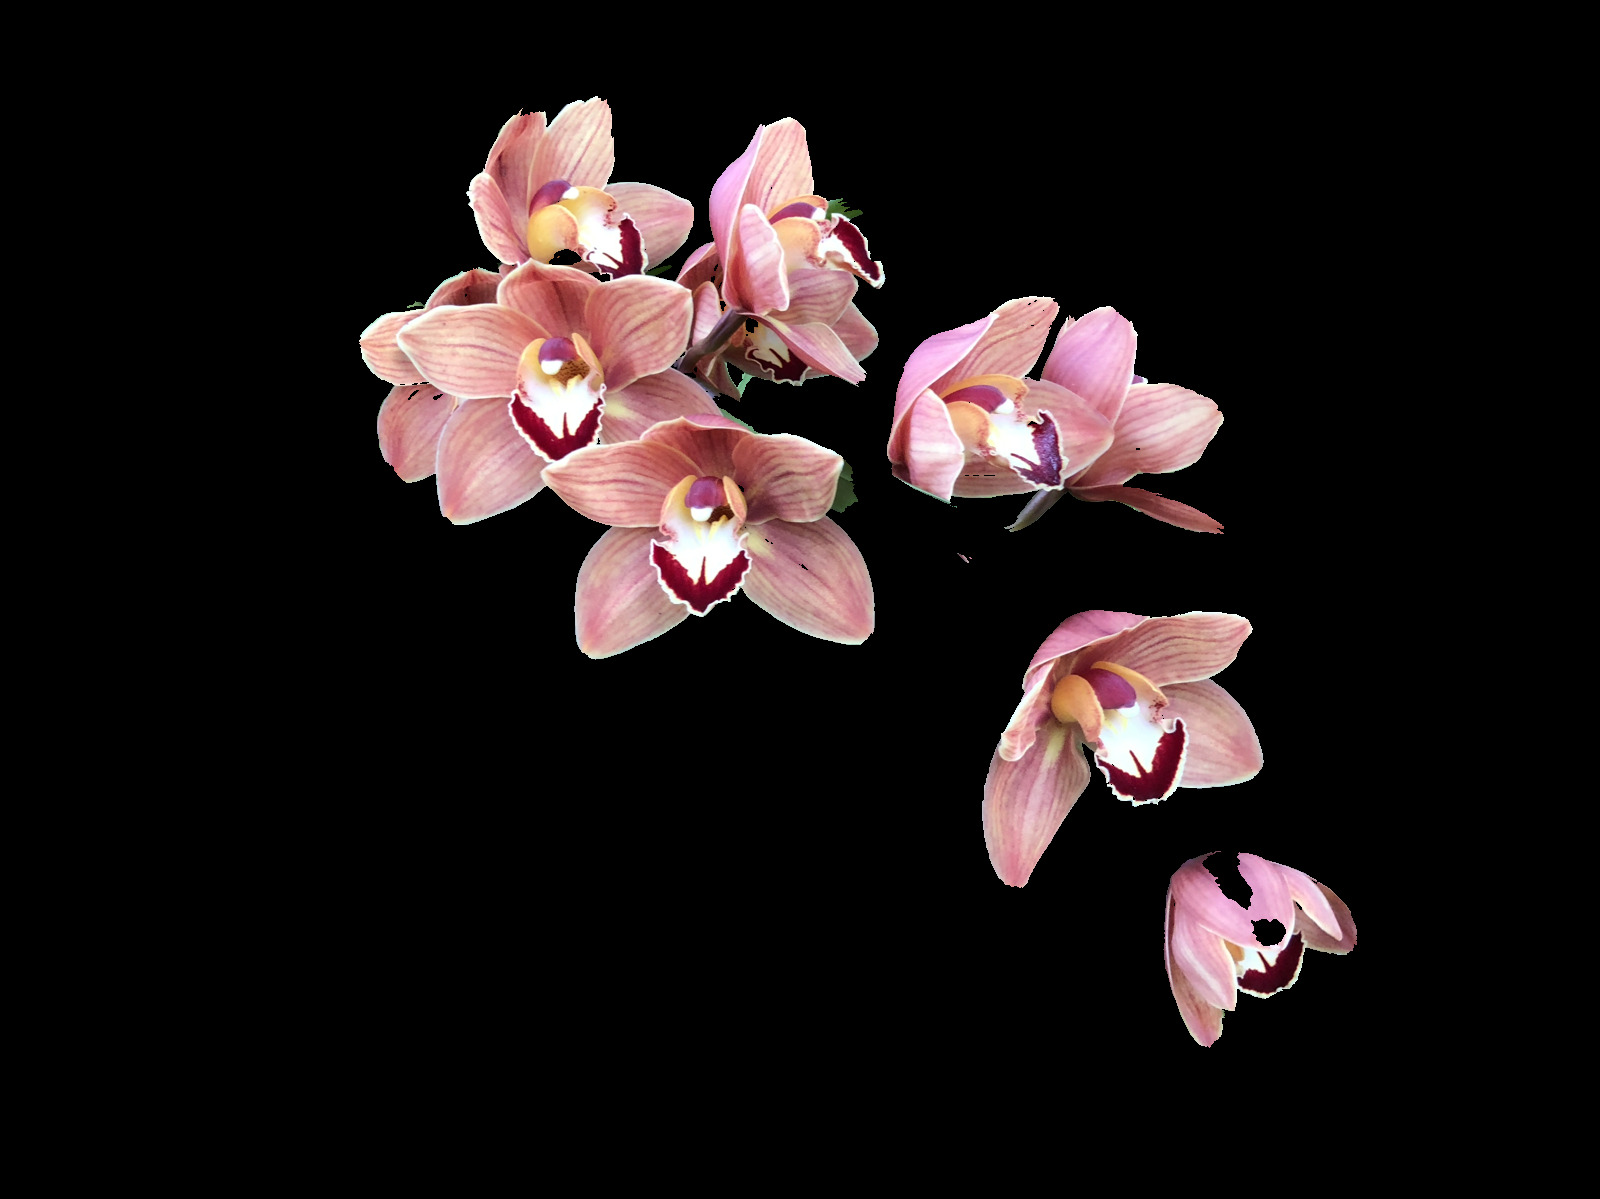
\includegraphics[width=\linewidth]{figures/nvos/orchids_dinov2.jpg}
        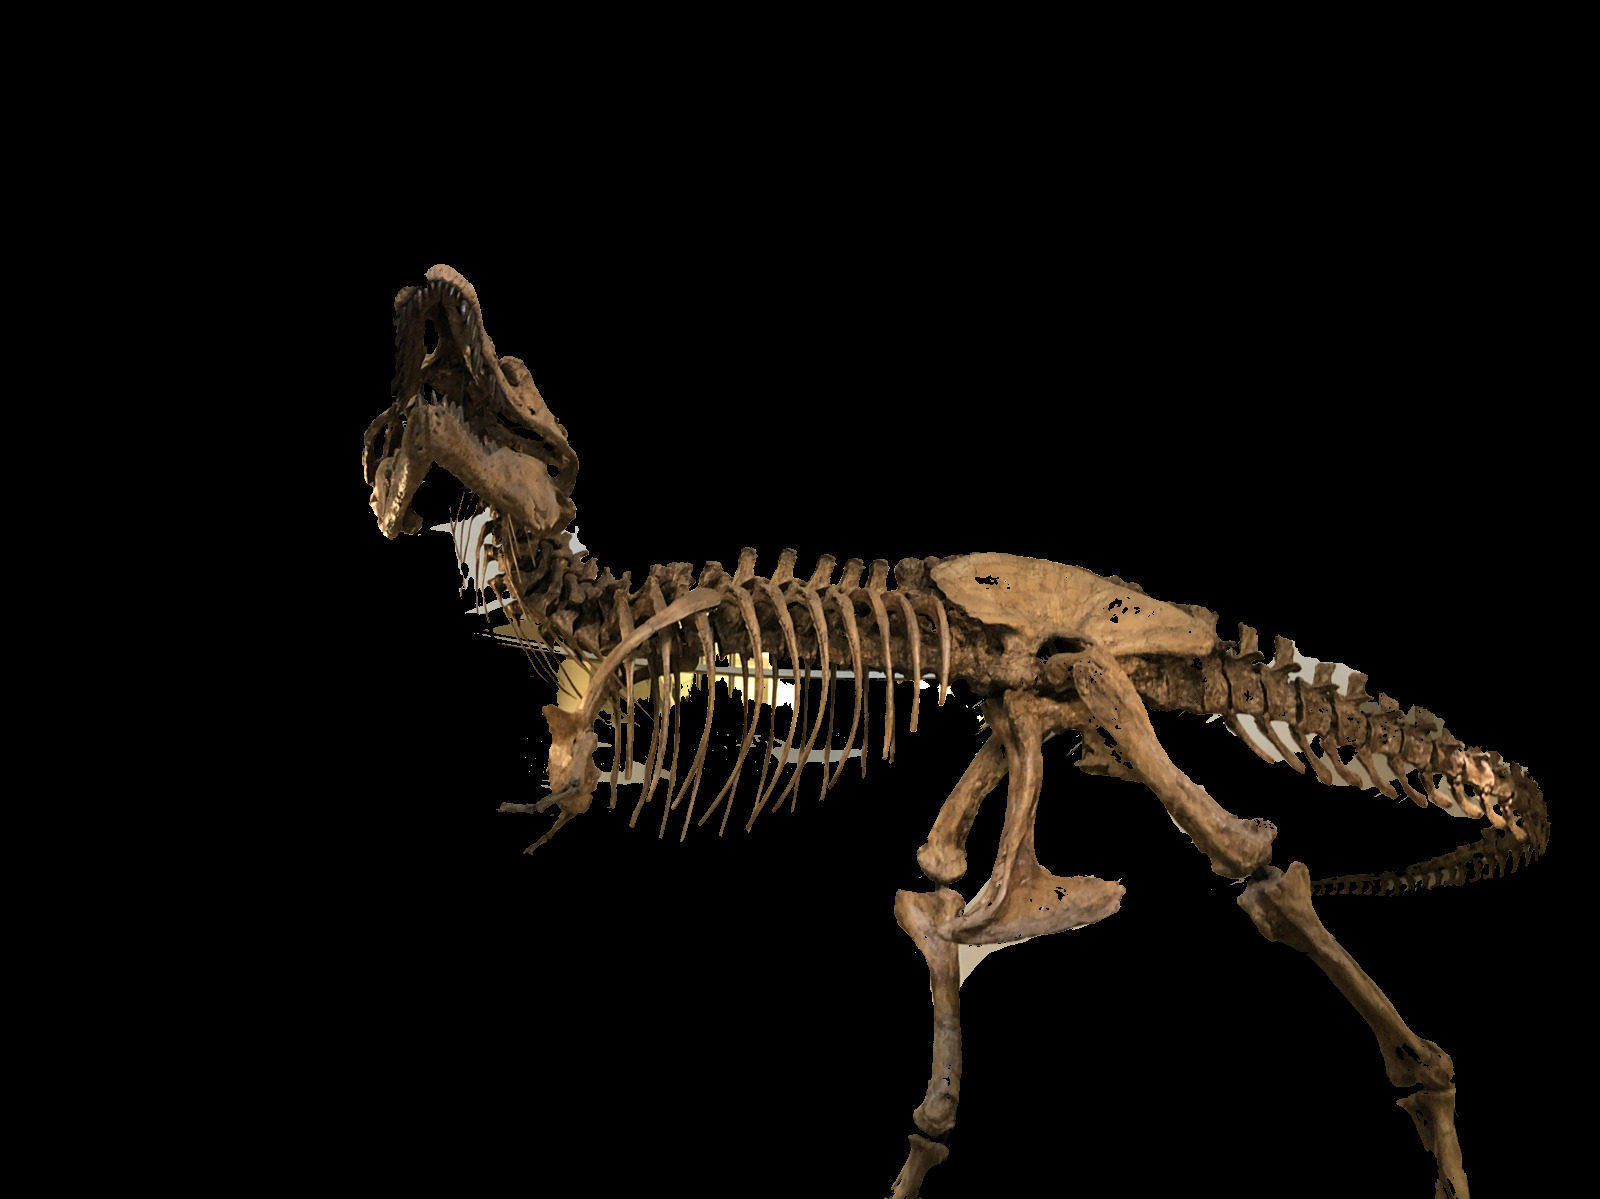
\includegraphics[width=\linewidth]{figures/nvos/trex_dinov2.jpg}
        \caption{SAM mask}
    \end{subfigure}
    \caption{Segmentation results on NVOS~\citep{ren2022nvos} with DINOv2 and SAM.}
    \label{fig:appendix-nvos}
\end{figure*}

\myparagraph{Diffusion process}
Fig.~\ref{fig:appendix-diffusion} illustrates different steps of the diffusion process for Fern, Leaves, Flower and Trex from the NVOS~\citep{ren2022nvos} dataset. Starting from the reference scribbles, the diffusion rapidly spreads through the large neighboring Gaussians. Covering the entire object takes more time for complex structures such as Fern, or for masks with disconnected components such as Orchids. As illustrated in the case of Flower, the last diffusion steps allow spreading to the smaller Gaussians on the flowers' edges, yielding a refined segmentation mask. For Trex, the parts being reached the latest are the head and tail. Their features are further away from the reference features (defined as the average feature over 3D reference scribbles), and therefore the regularization for diffusion is stronger in these regions. Overall once the object has been fully covered, the regularization is very effective at preventing leakage, which allows diffusion to run for an arbitrary number of steps.

\begin{figure*}[t!]
    \centering
    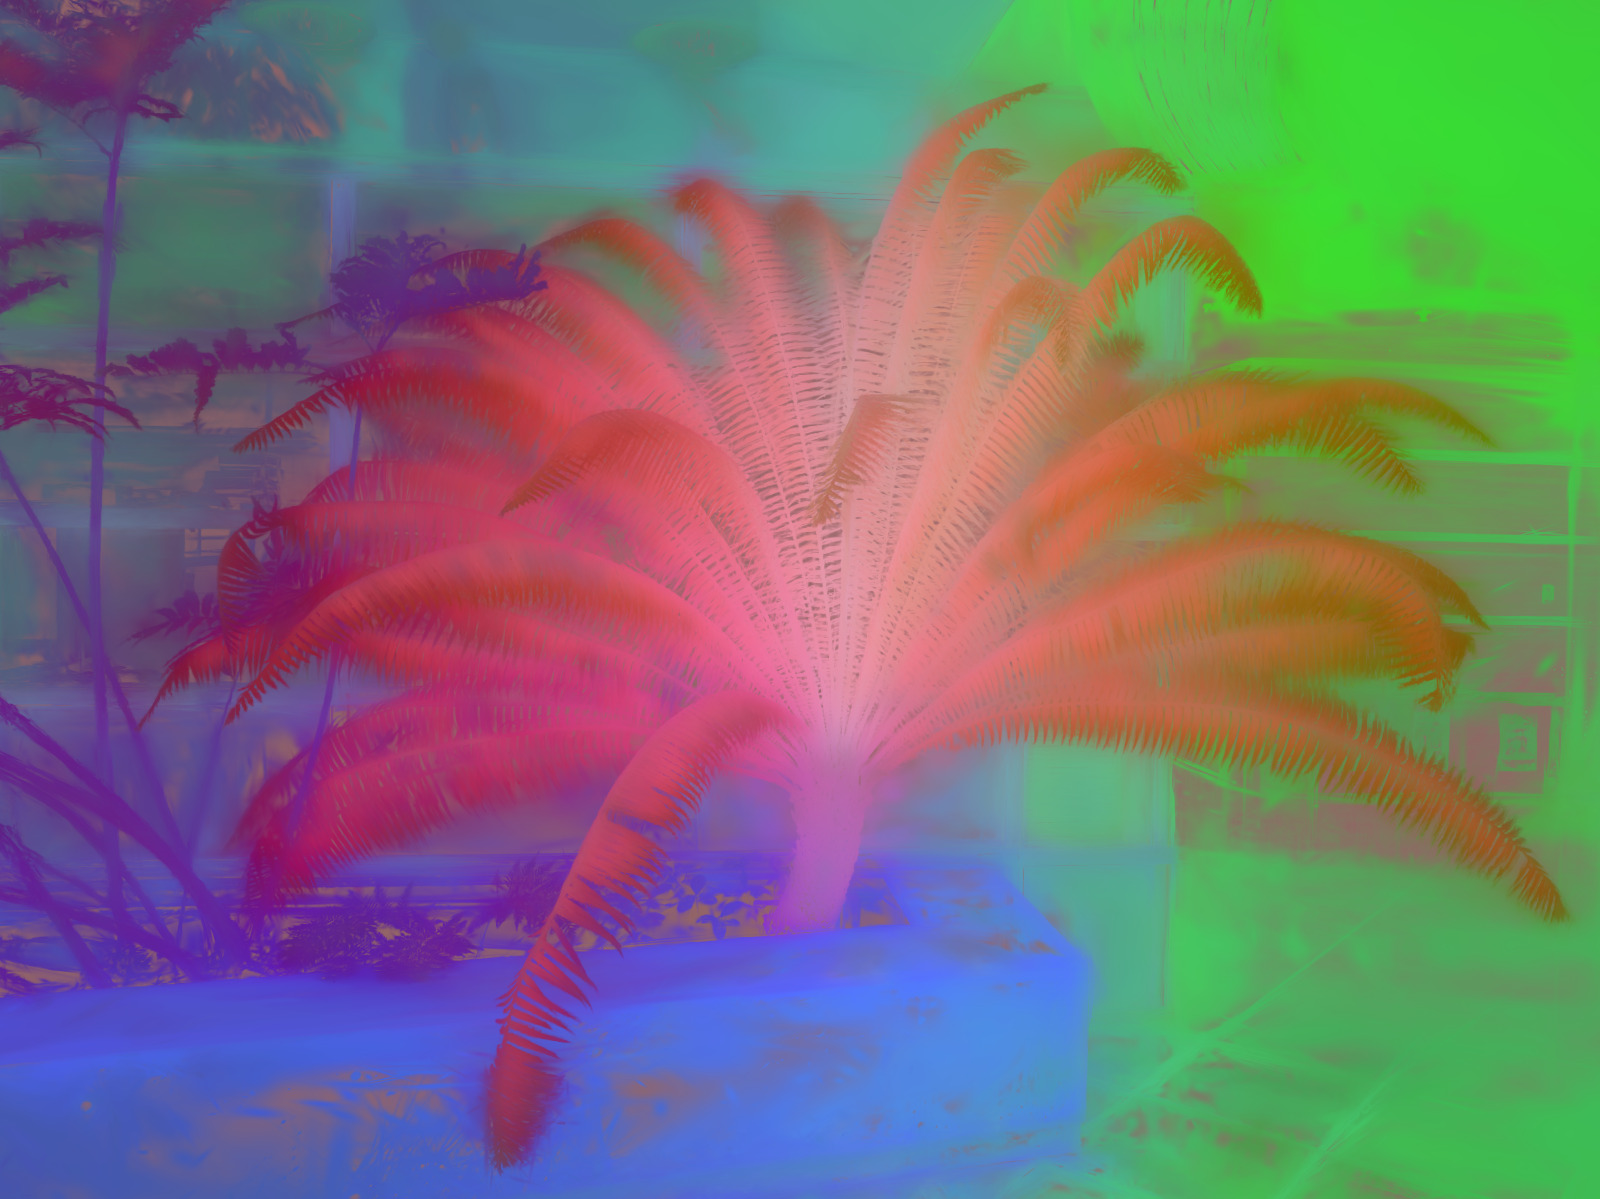
\includegraphics[width=0.2\linewidth]{figures/diffusion_appendix/fern_pca.jpg}
    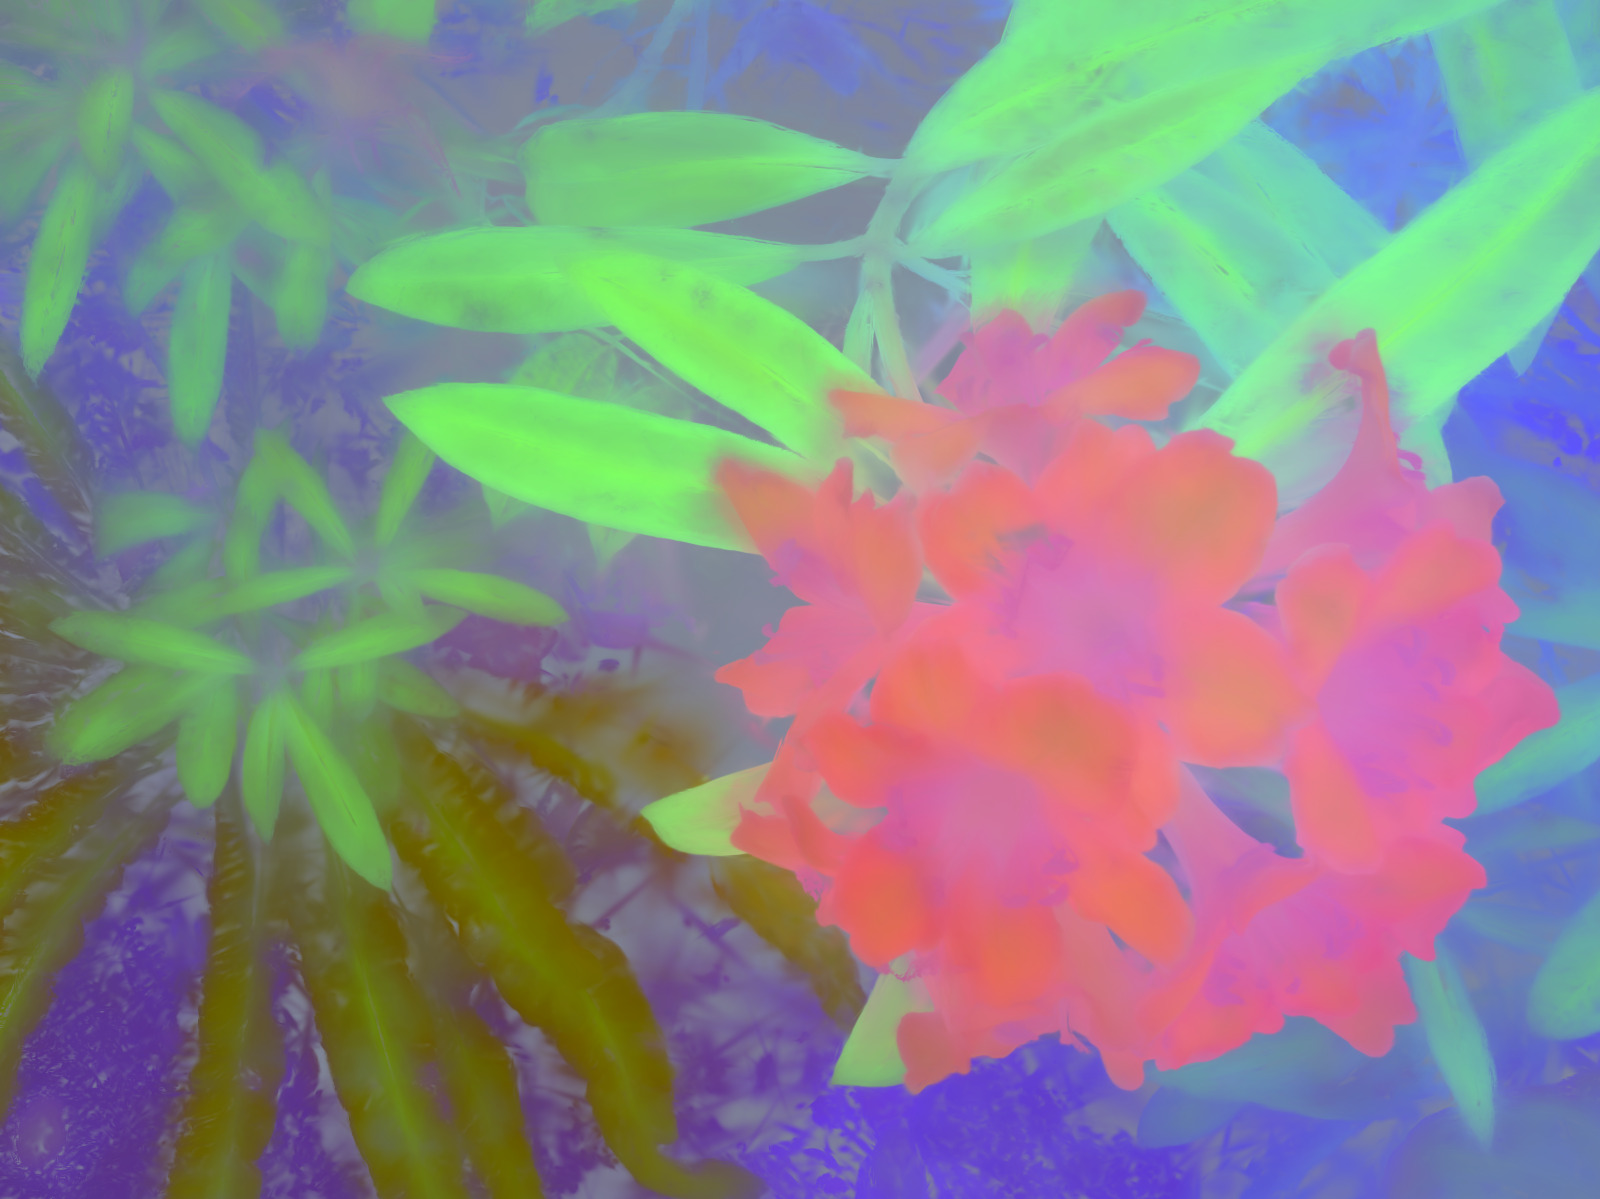
\includegraphics[width=0.2\linewidth]{figures/diffusion_appendix/flower_pca.jpg}
    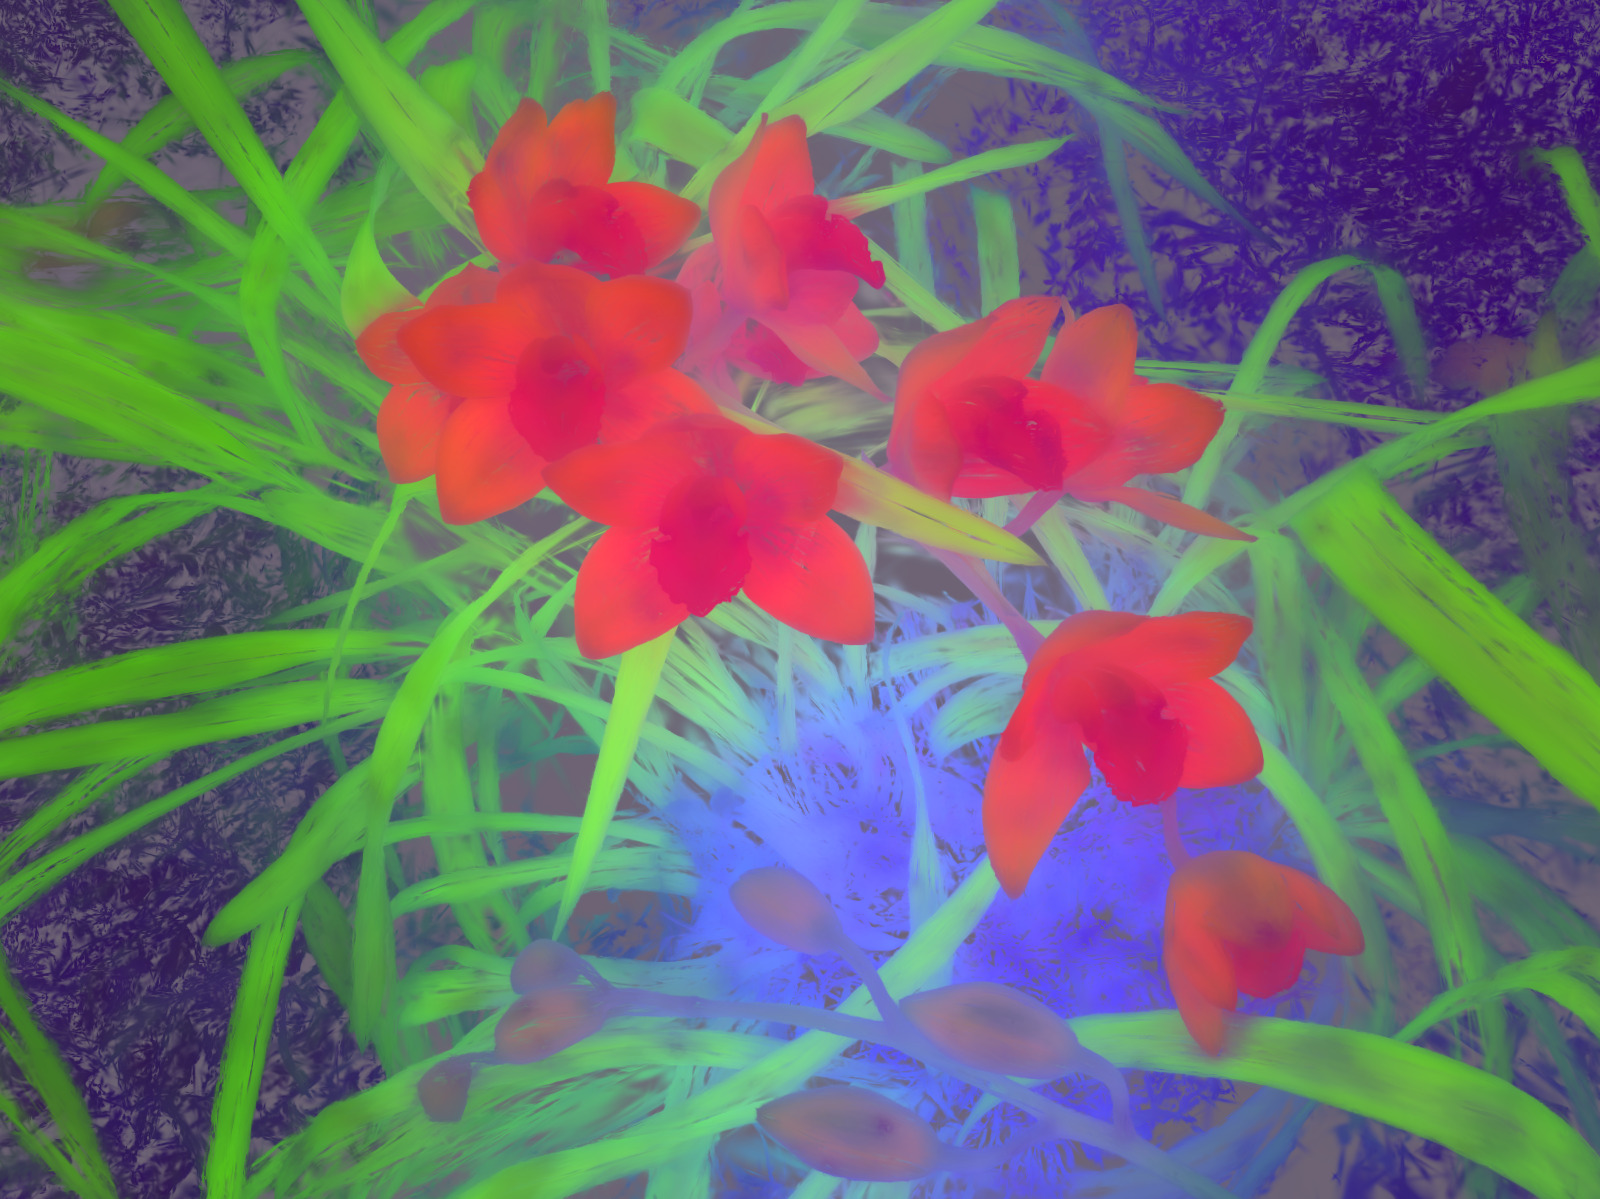
\includegraphics[width=0.2\linewidth]{figures/pcas/orchids_pca.jpg}
    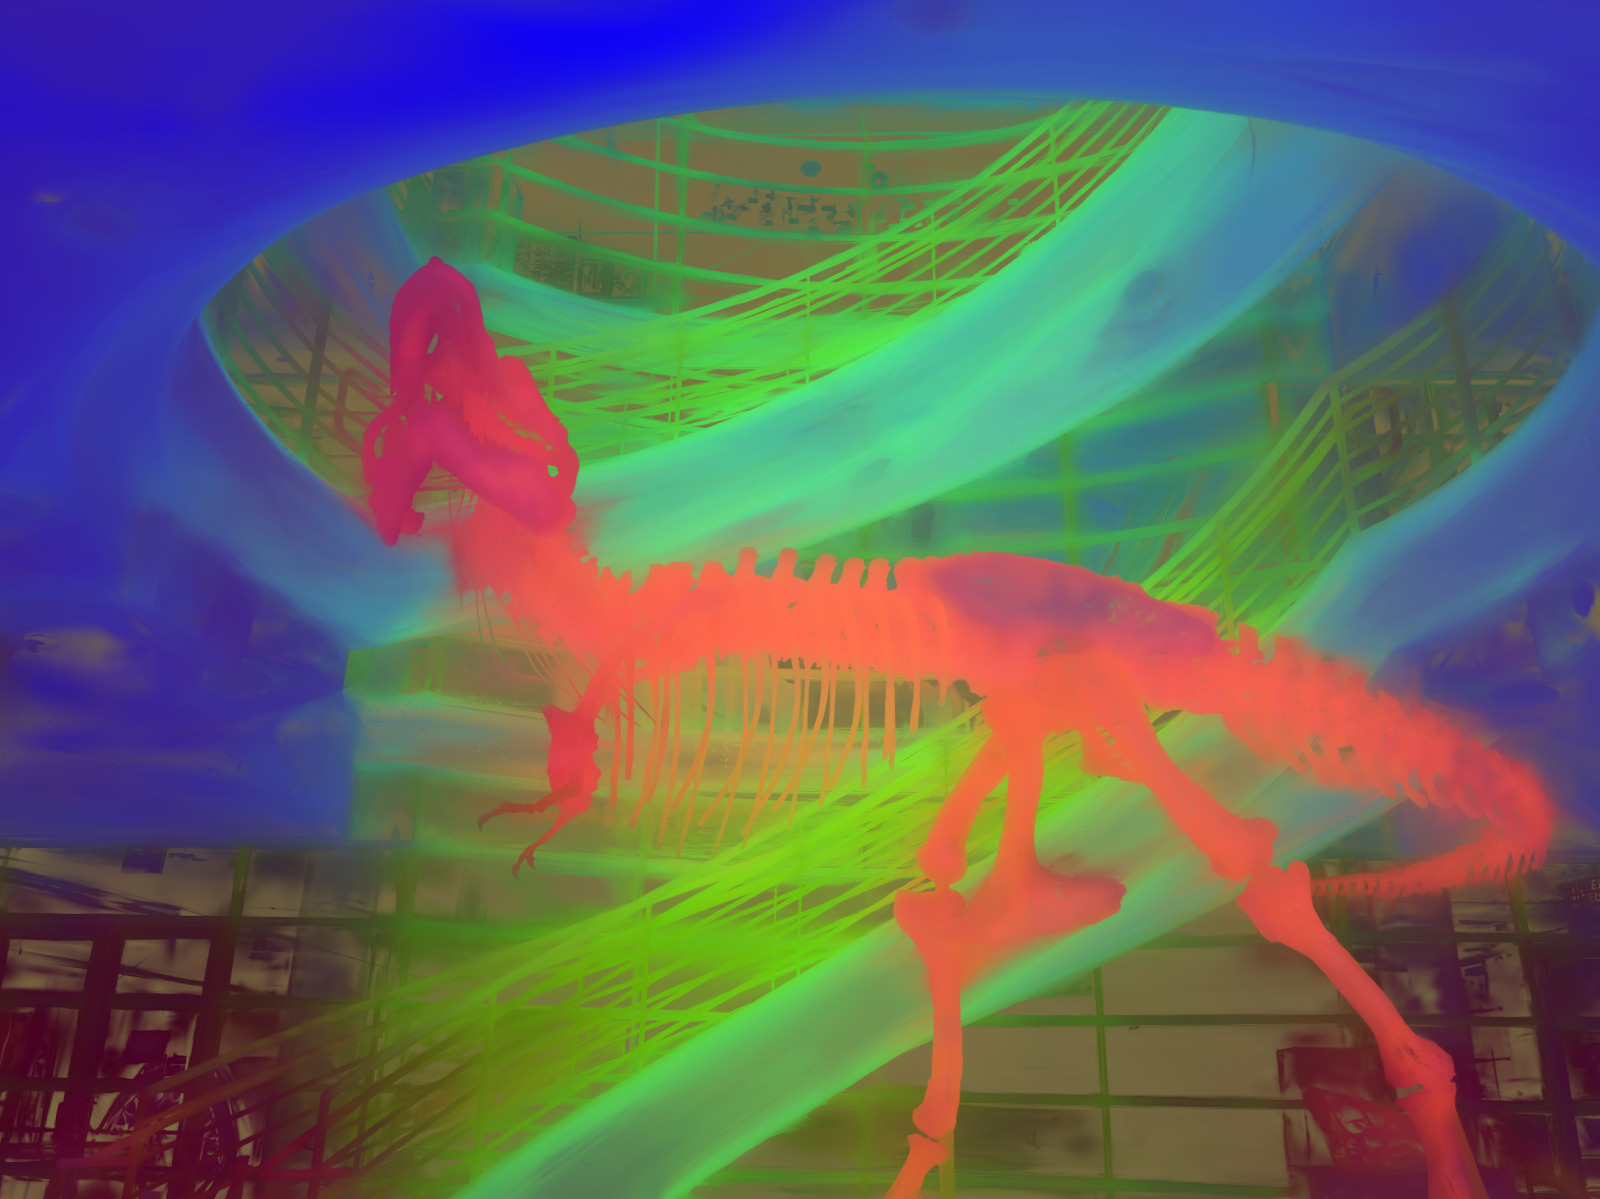
\includegraphics[width=0.2\linewidth]{figures/pcas/trex_pca.jpg} \\
    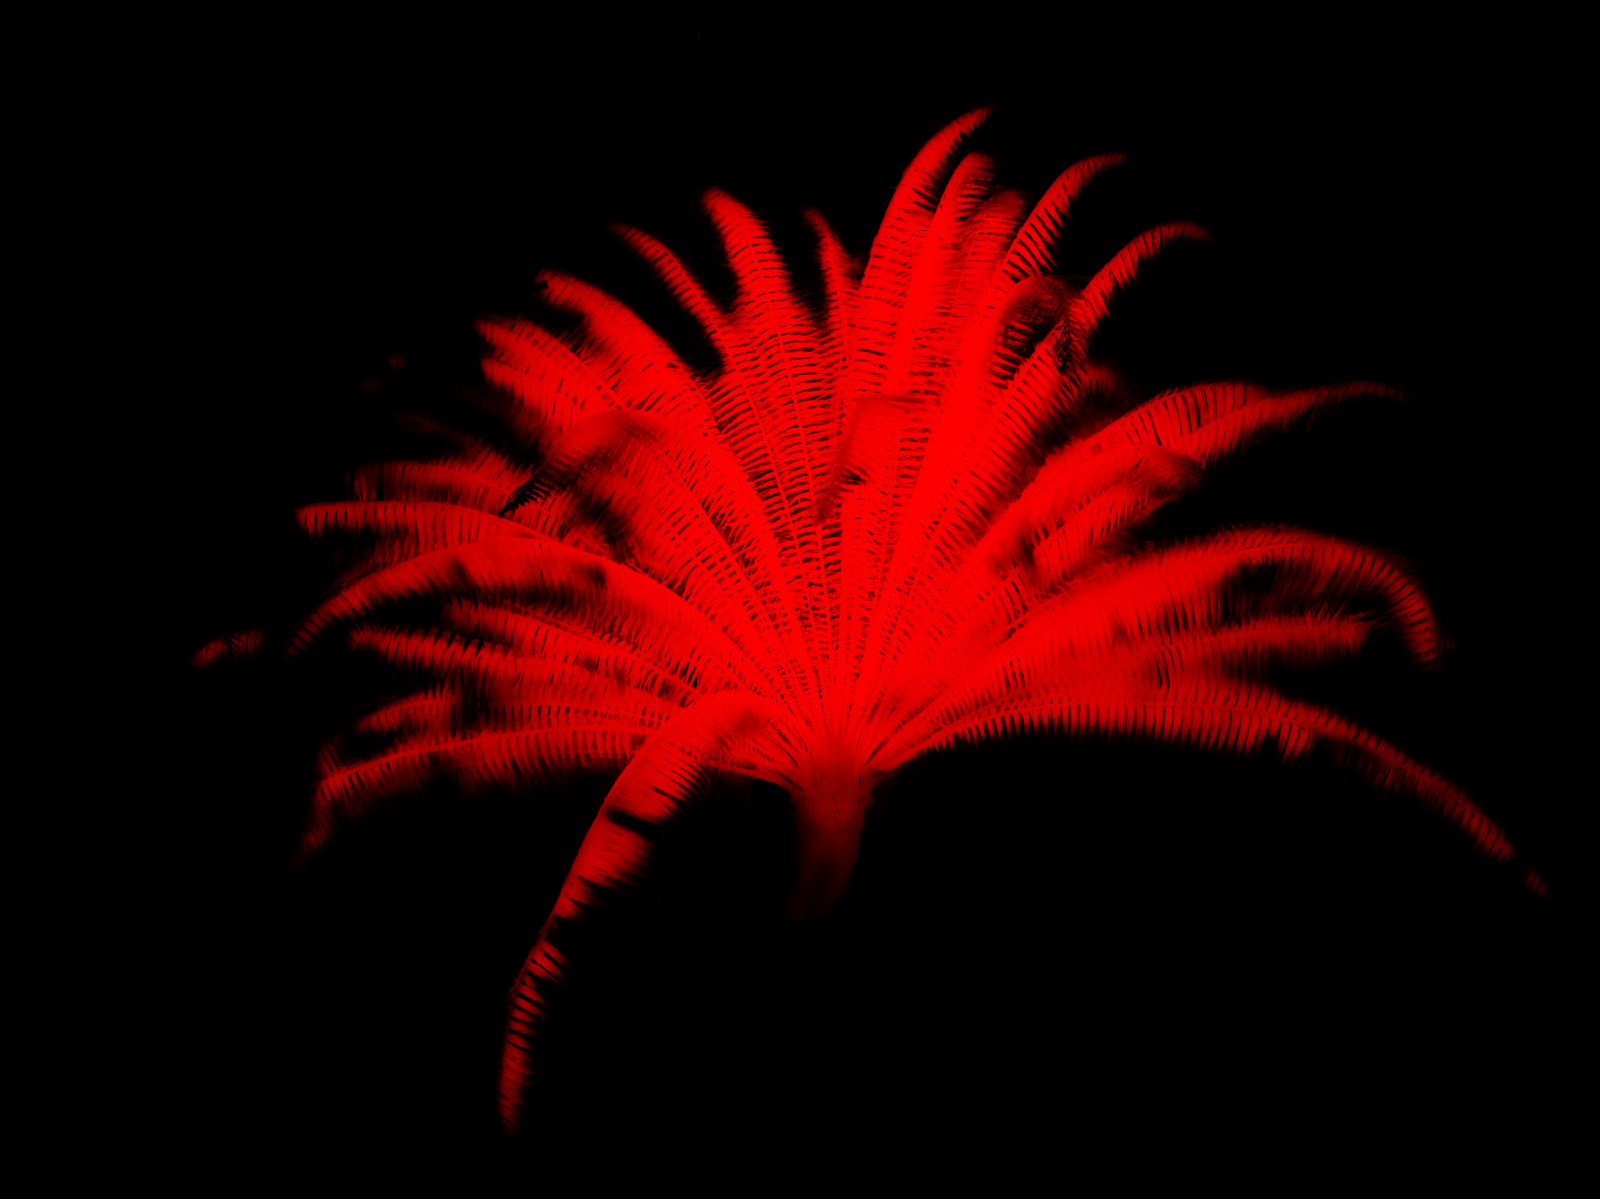
\includegraphics[width=0.2\linewidth]{figures/diffusion_appendix/fern_regularizer.jpg}
    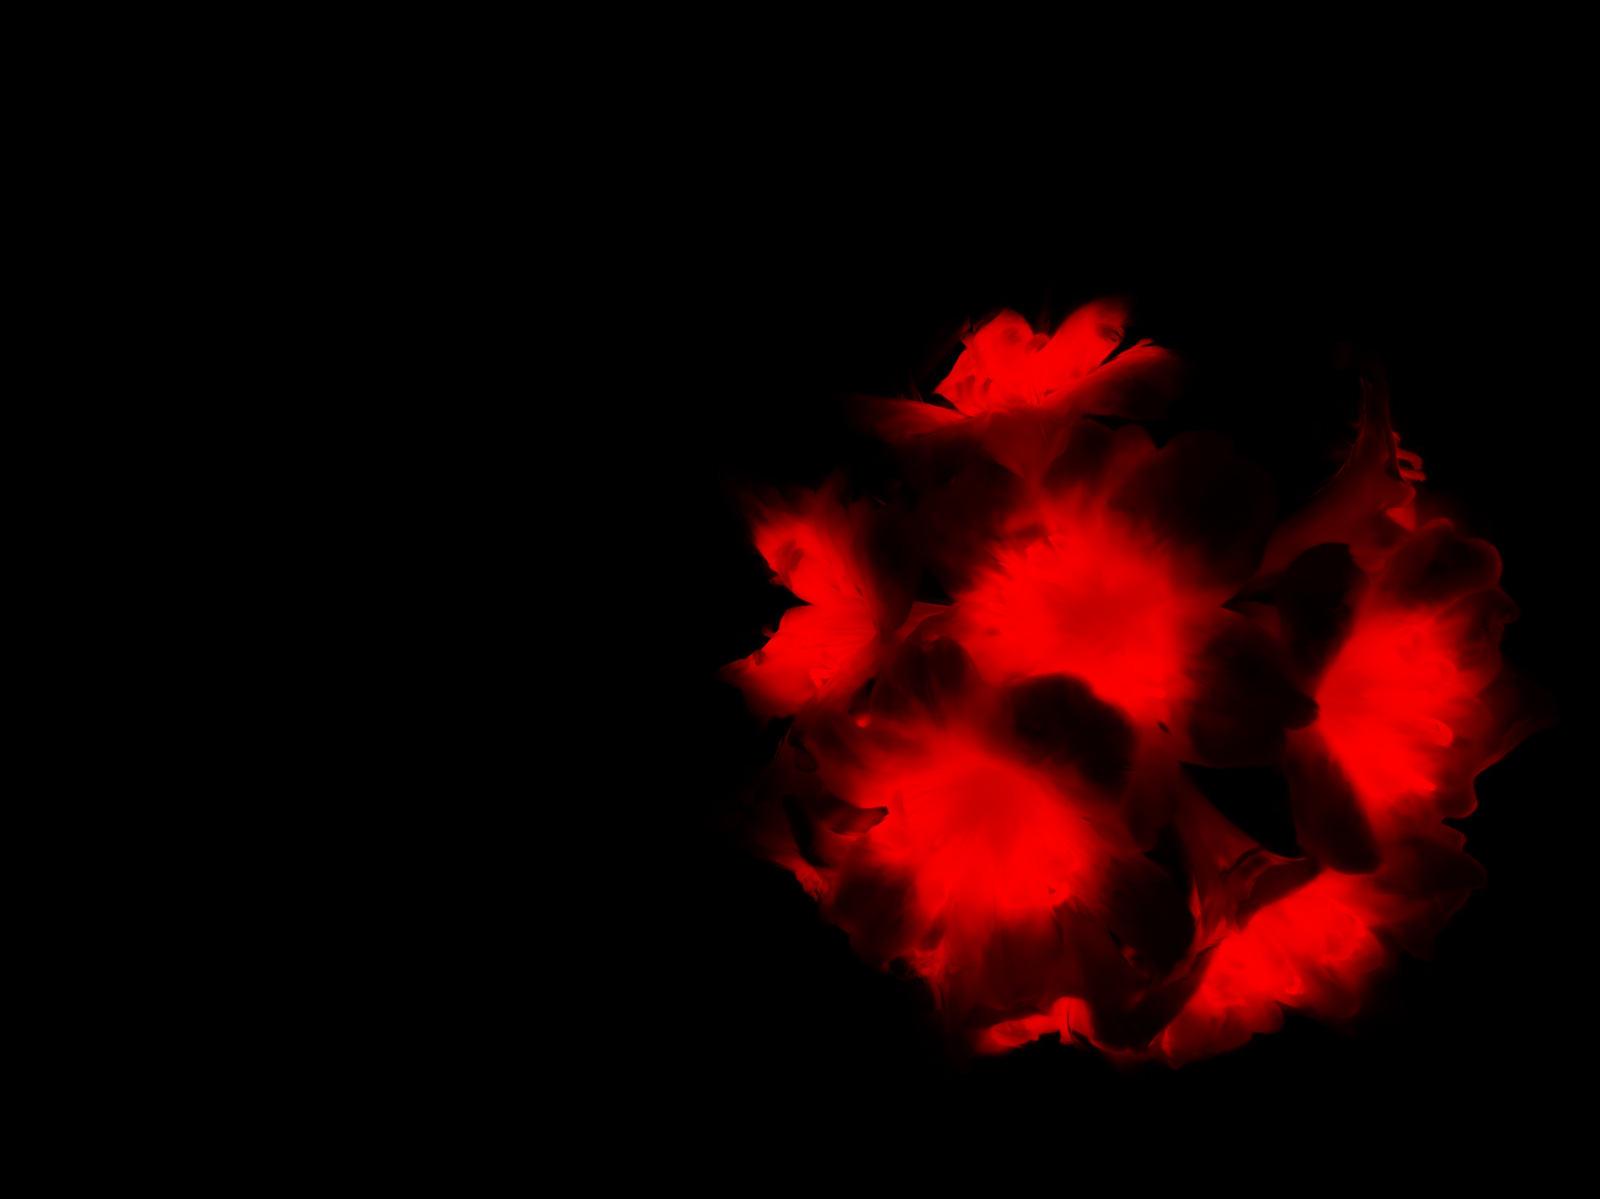
\includegraphics[width=0.2\linewidth]{figures/diffusion_appendix/flower_regularizer.jpg}
    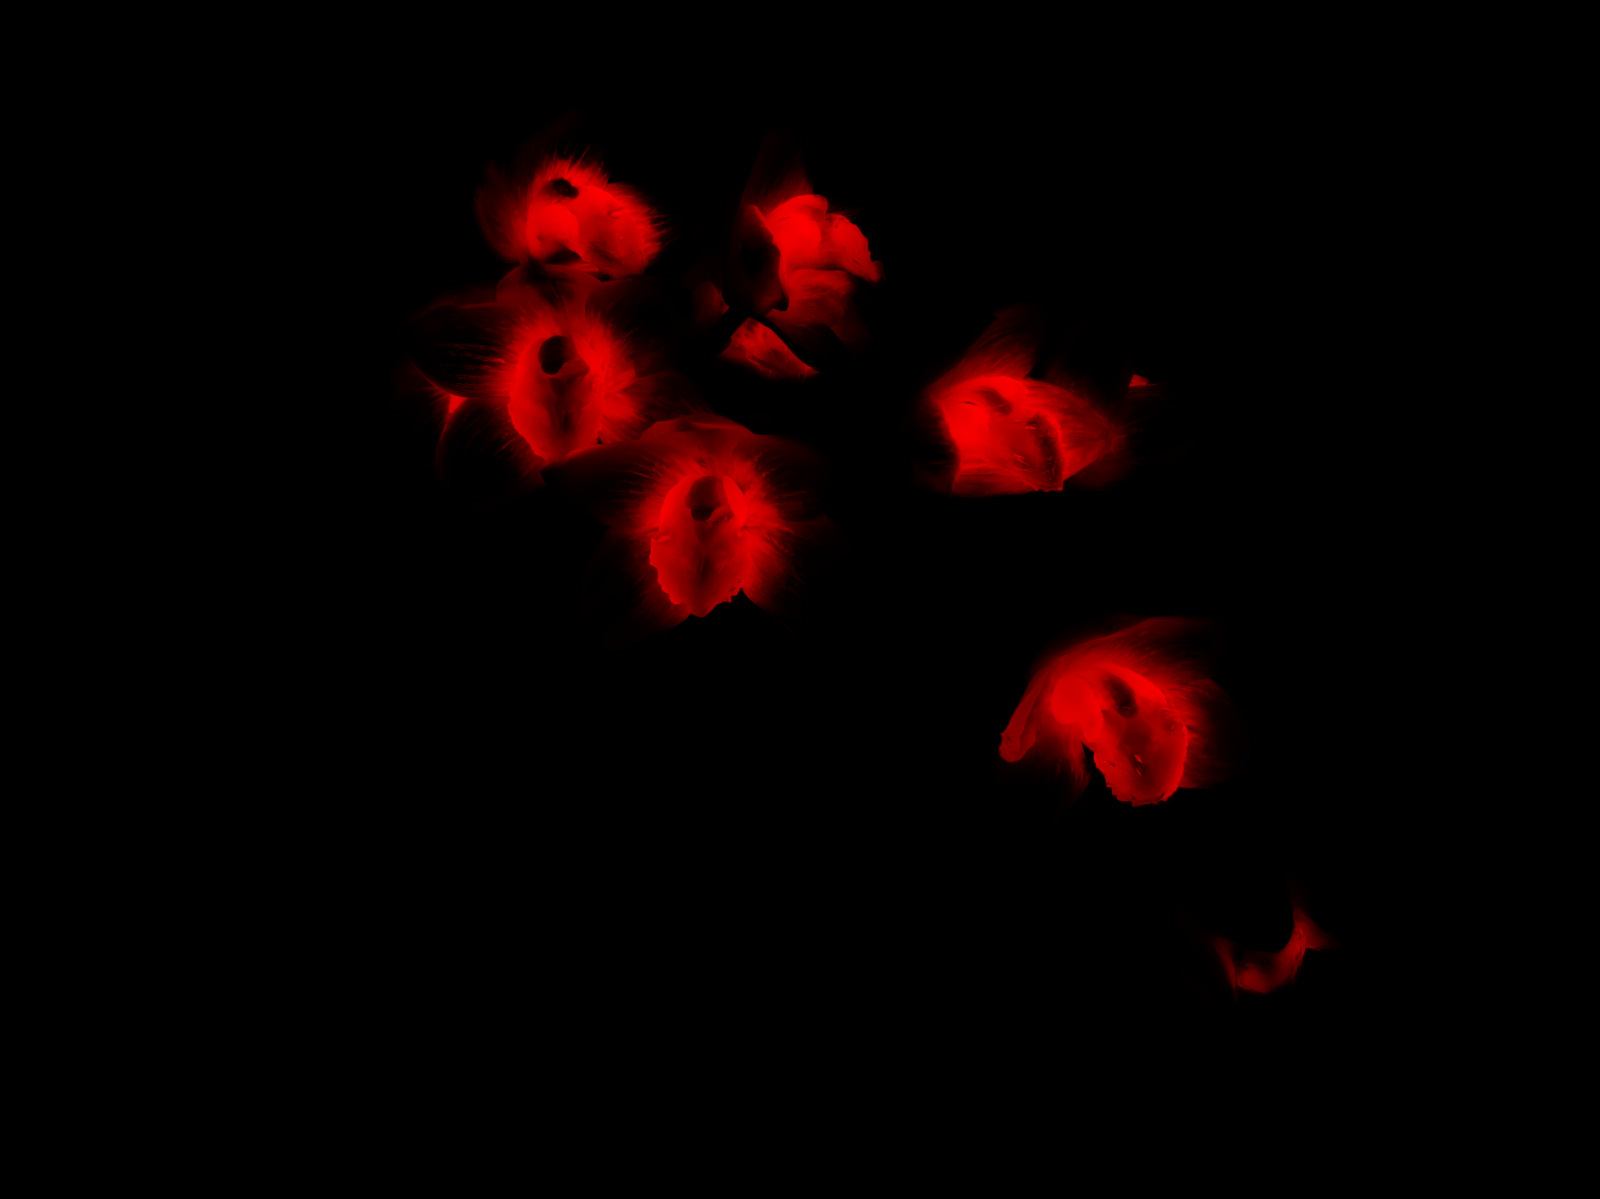
\includegraphics[width=0.2\linewidth]{figures/diffusion_appendix/orchids_regularizer.jpg}
    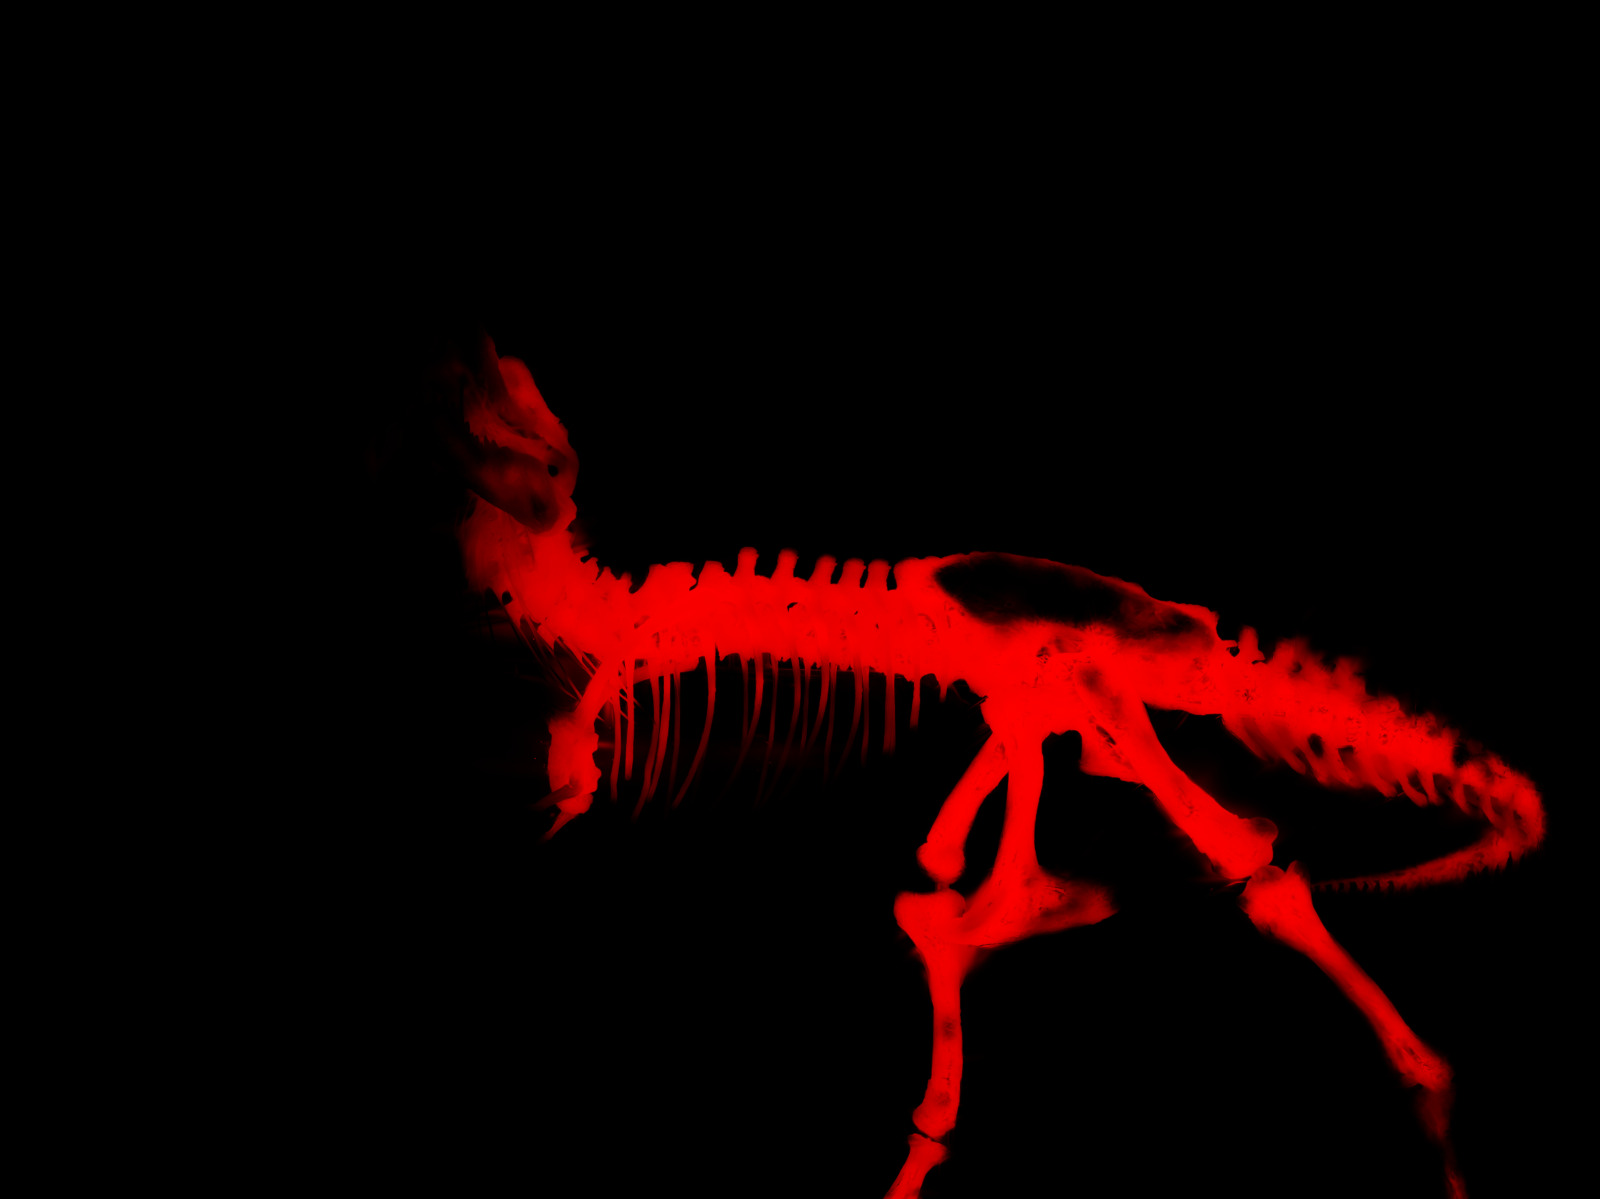
\includegraphics[width=0.2\linewidth]{figures/diffusion_appendix/trex_regularizer.jpg} \\
    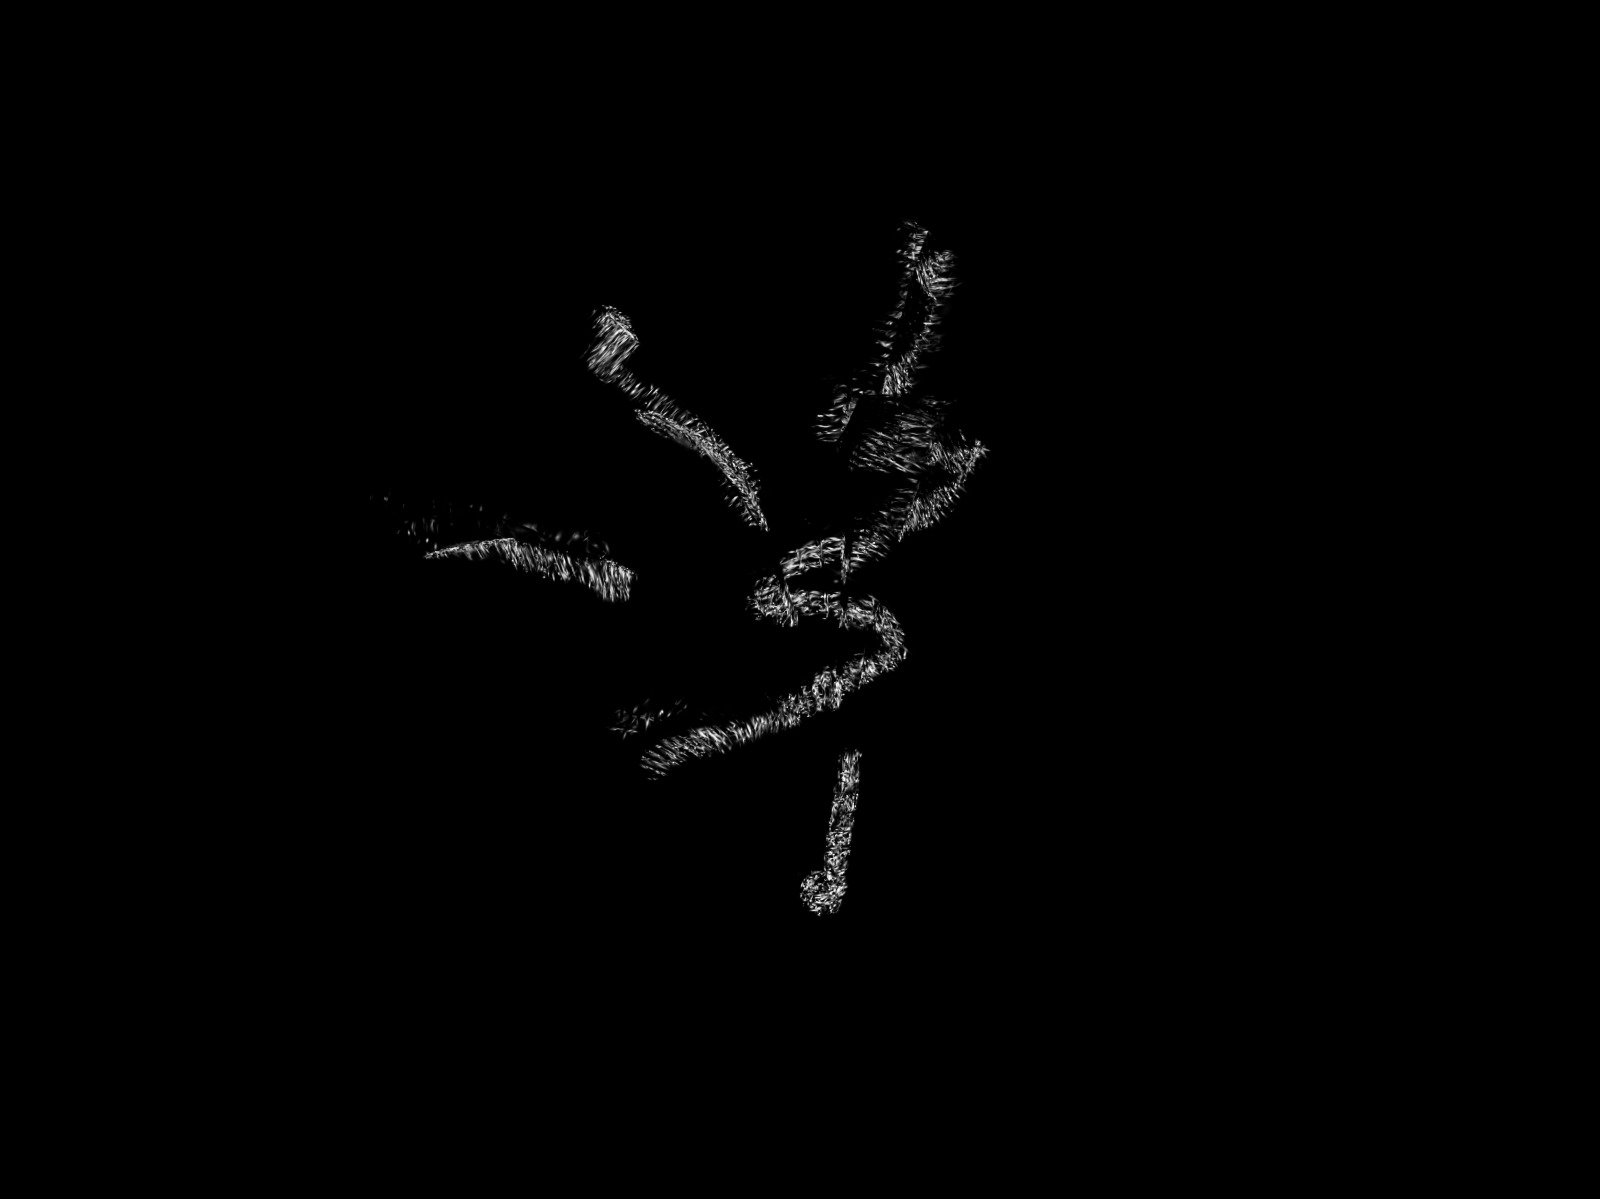
\includegraphics[width=0.2\linewidth]{figures/diffusion_appendix/fern_init.jpg}
    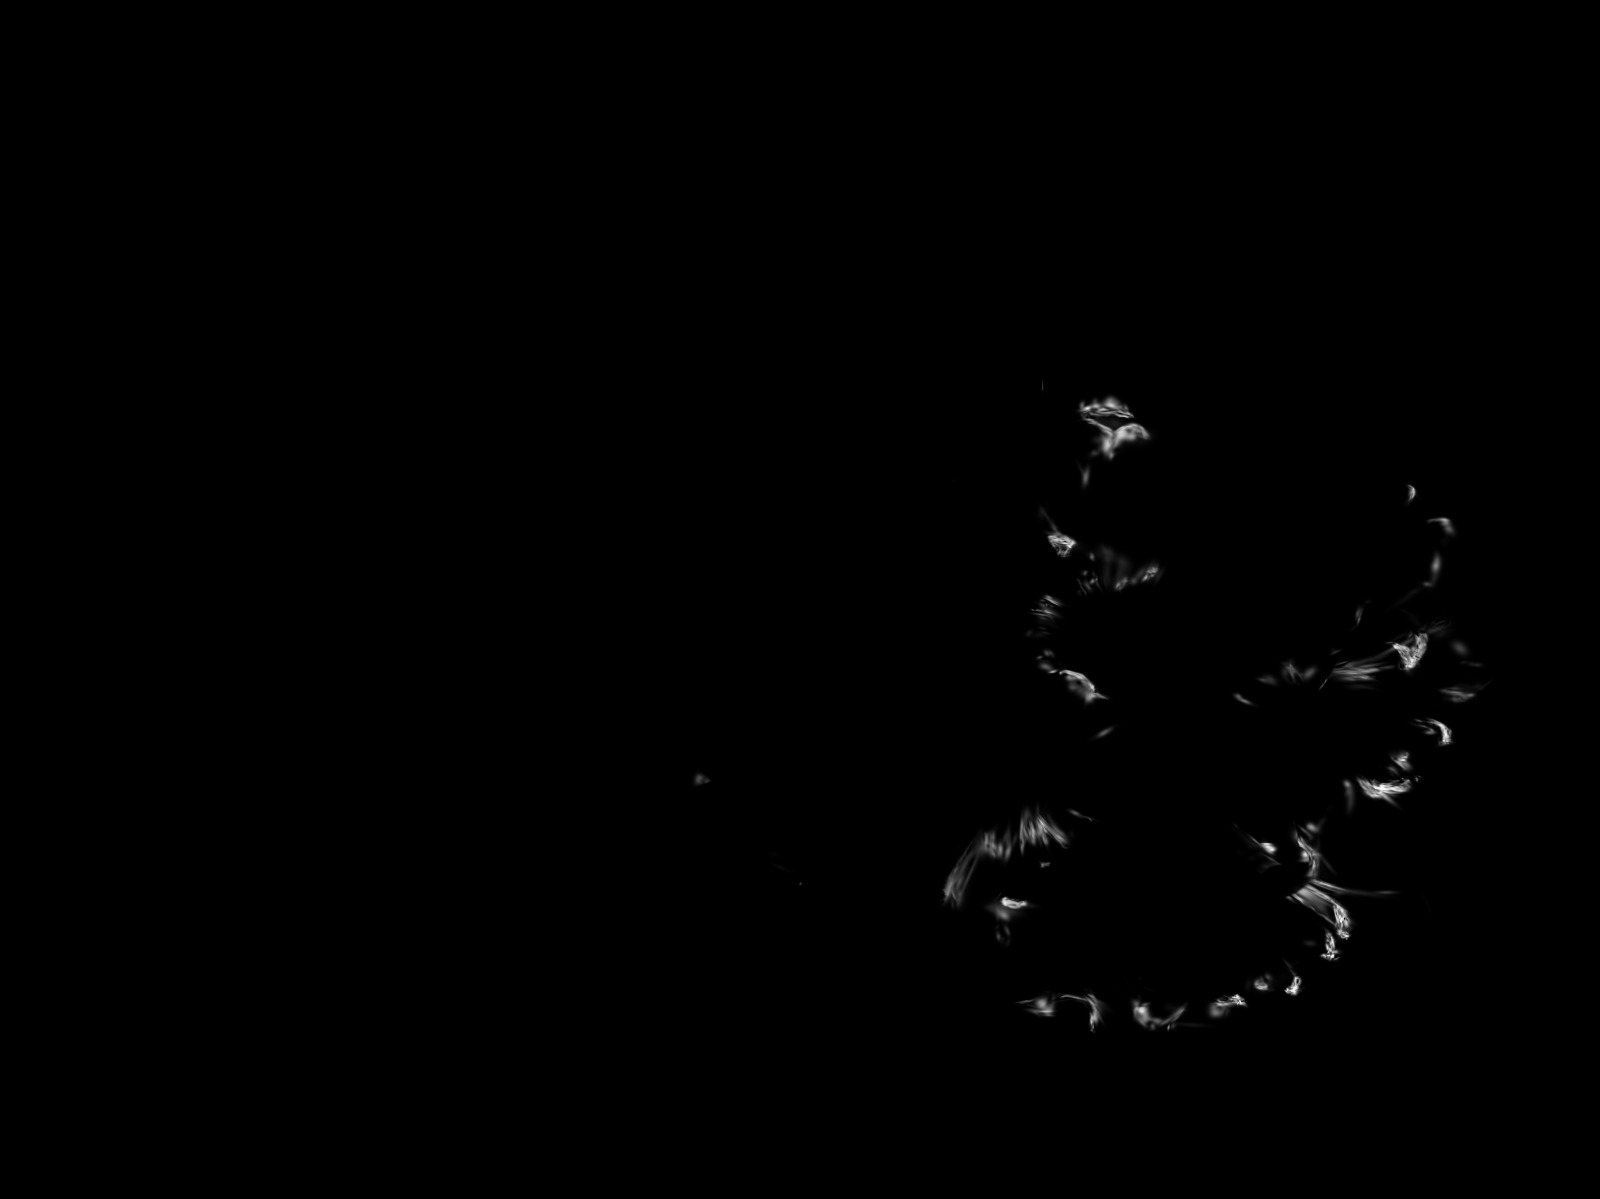
\includegraphics[width=0.2\linewidth]{figures/diffusion_appendix/flower_init.jpg}
    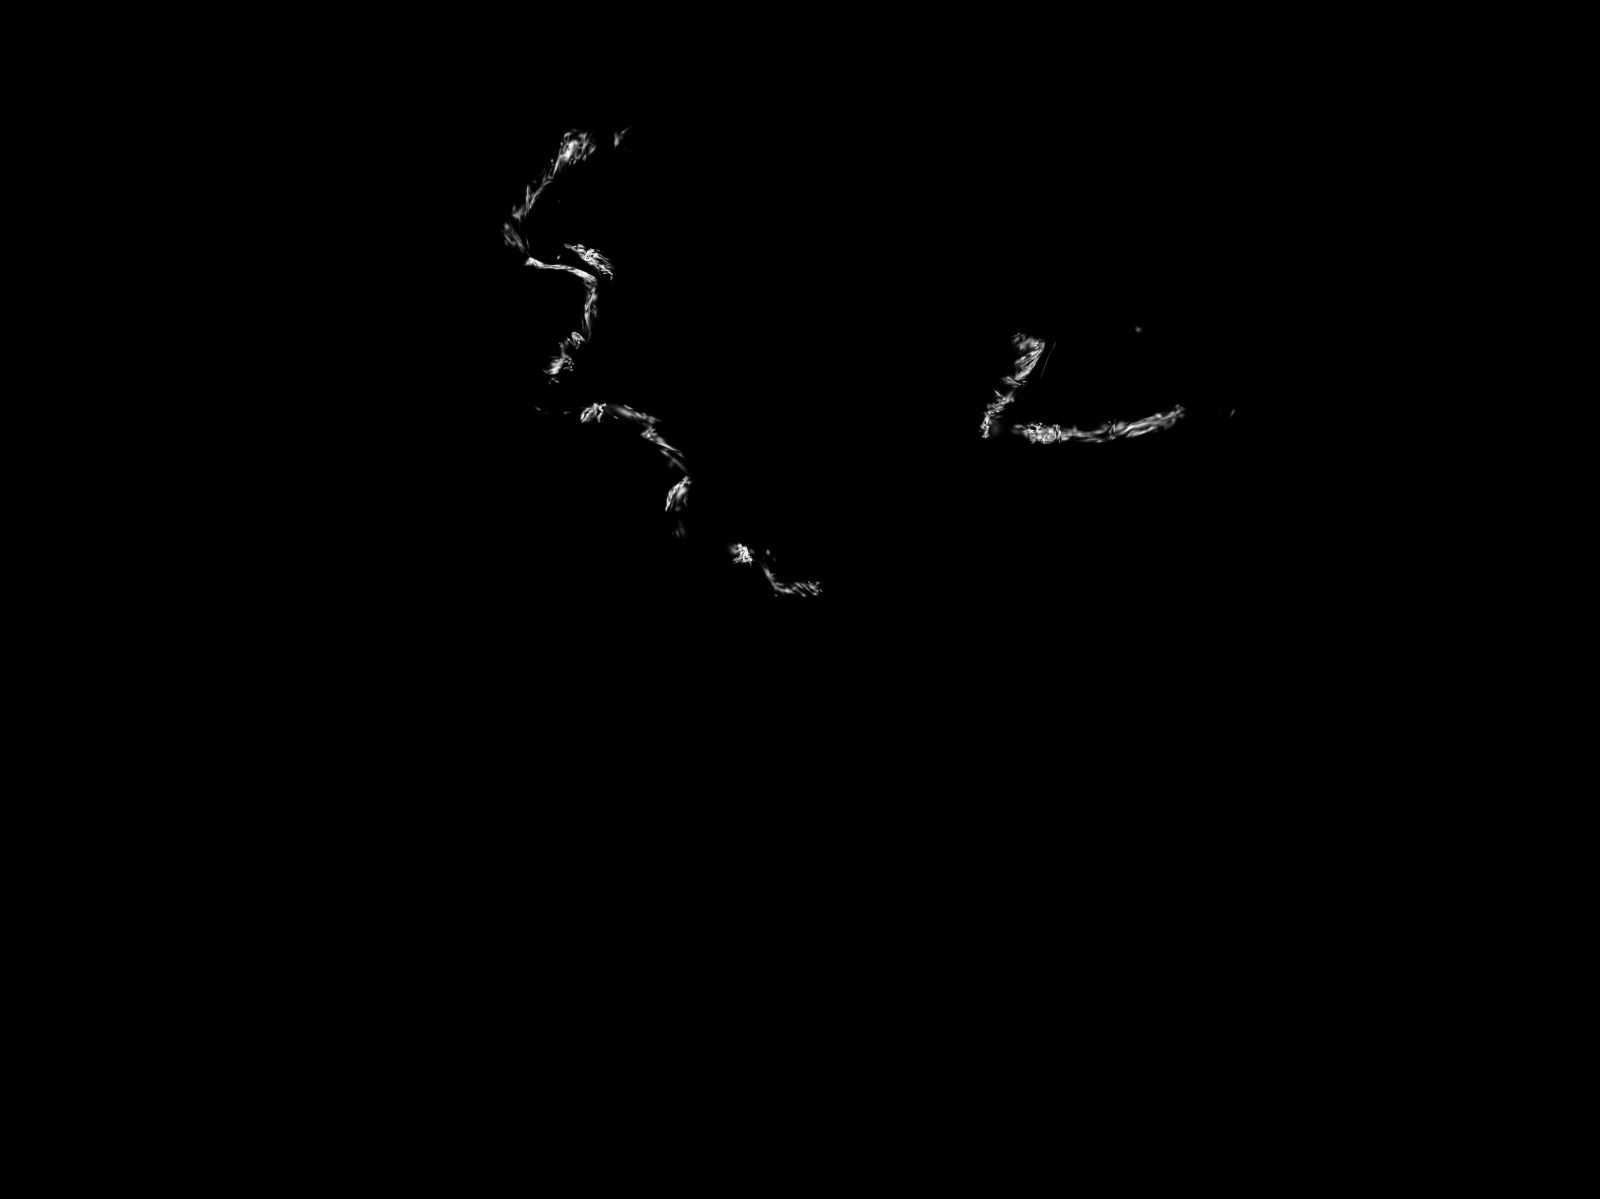
\includegraphics[width=0.2\linewidth]{figures/diffusion_appendix/orchids_init.jpg}
    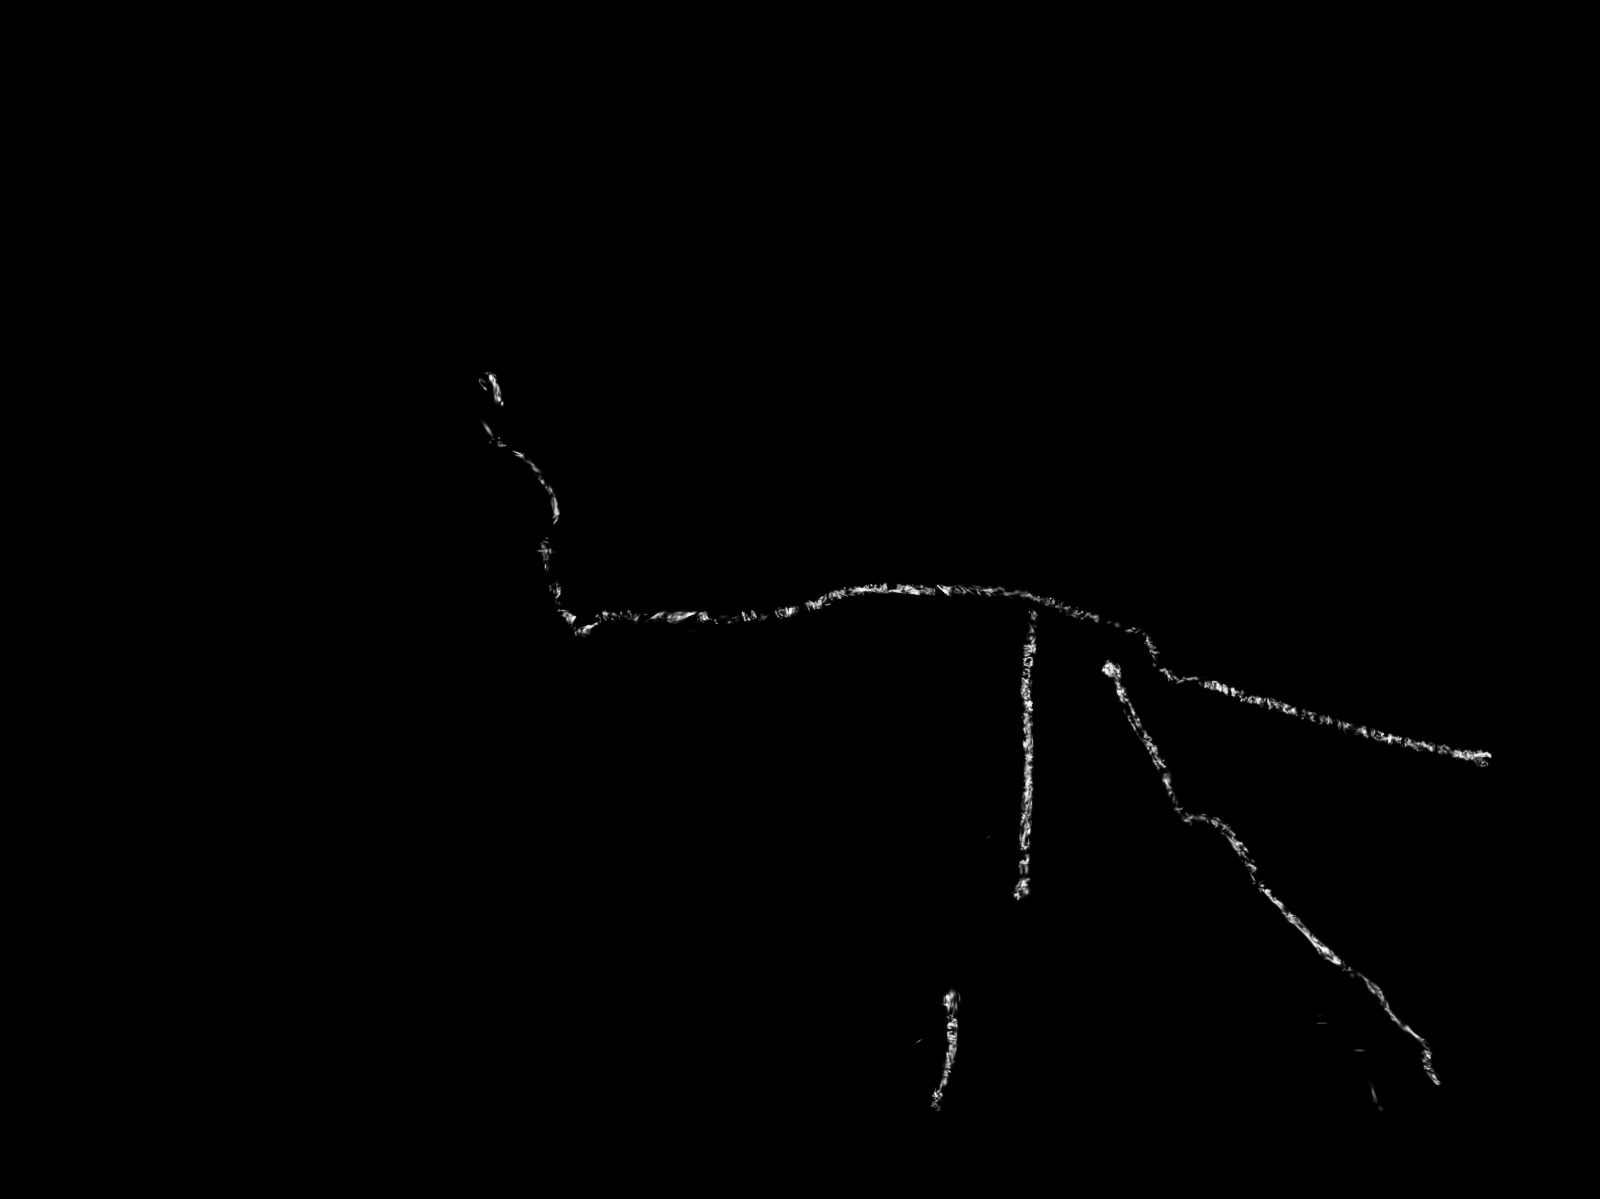
\includegraphics[width=0.2\linewidth]{figures/diffusion_appendix/trex_init.jpg} \\
    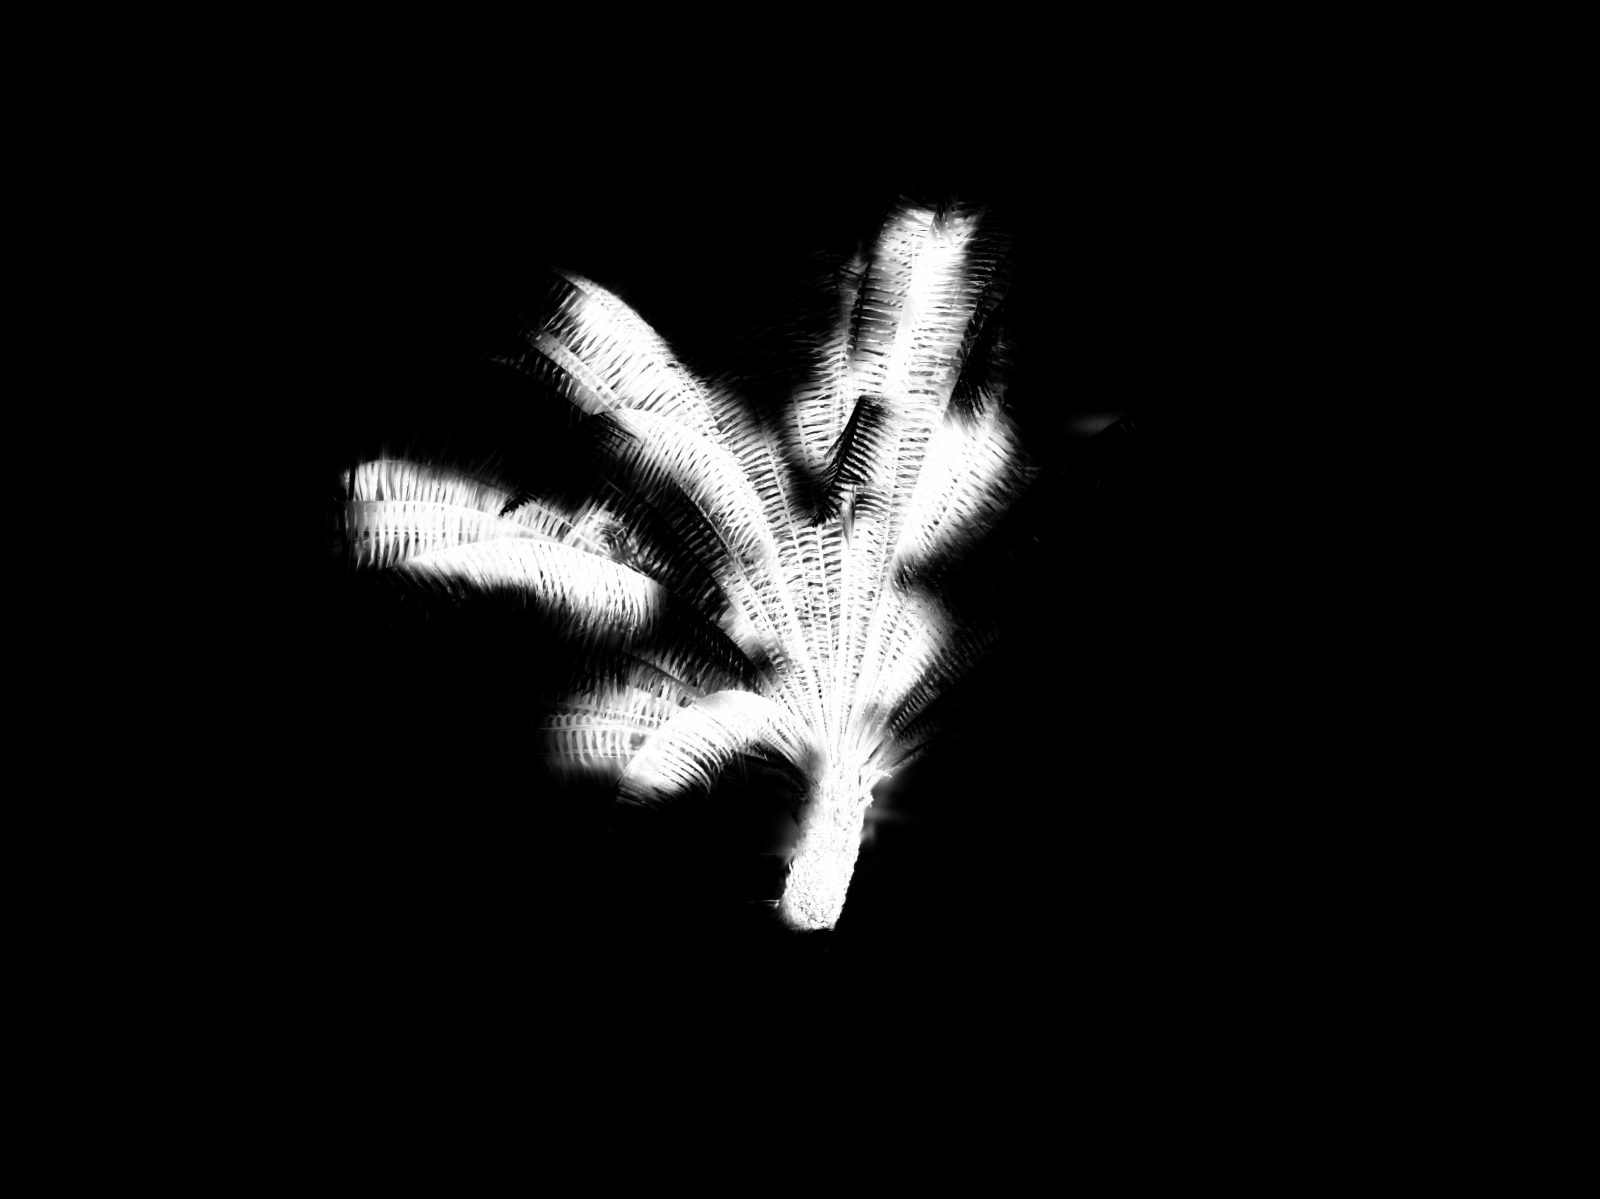
\includegraphics[width=0.2\linewidth]{figures/diffusion_appendix/fern_sim_3it.jpg}
    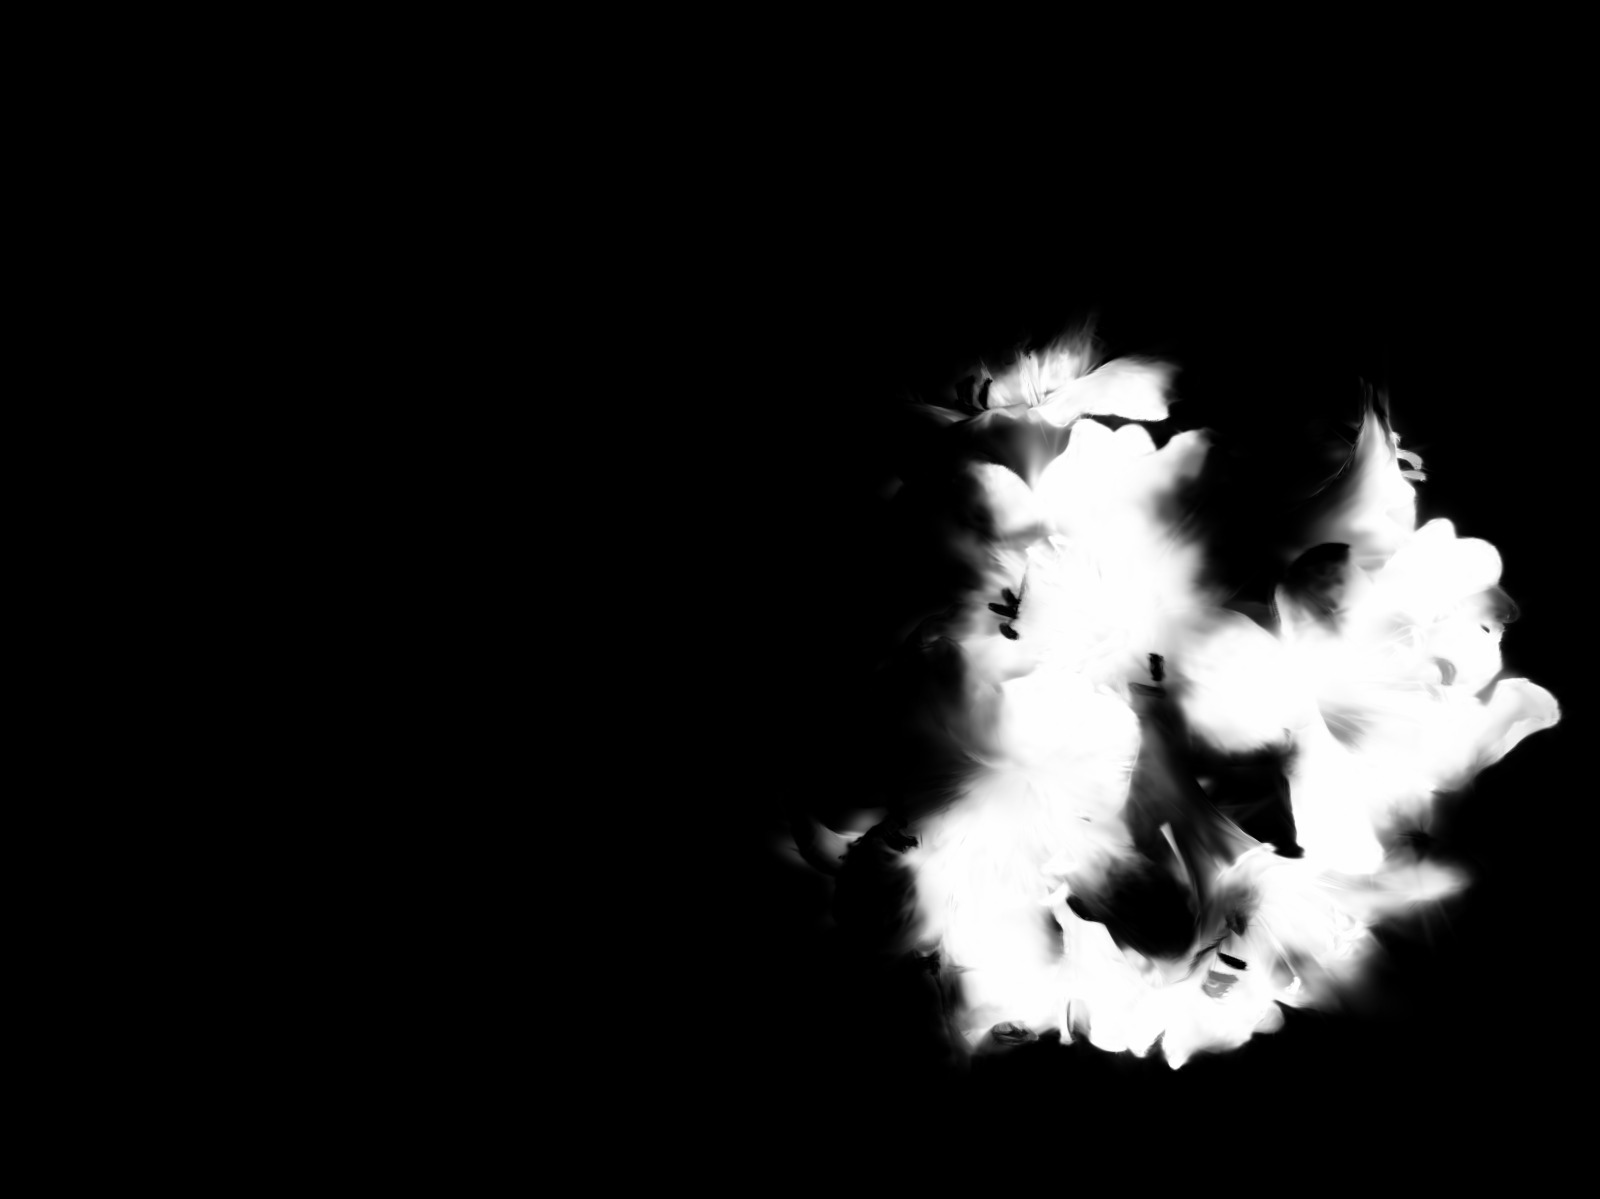
\includegraphics[width=0.2\linewidth]{figures/diffusion_appendix/flower_sim_3it.jpg}
    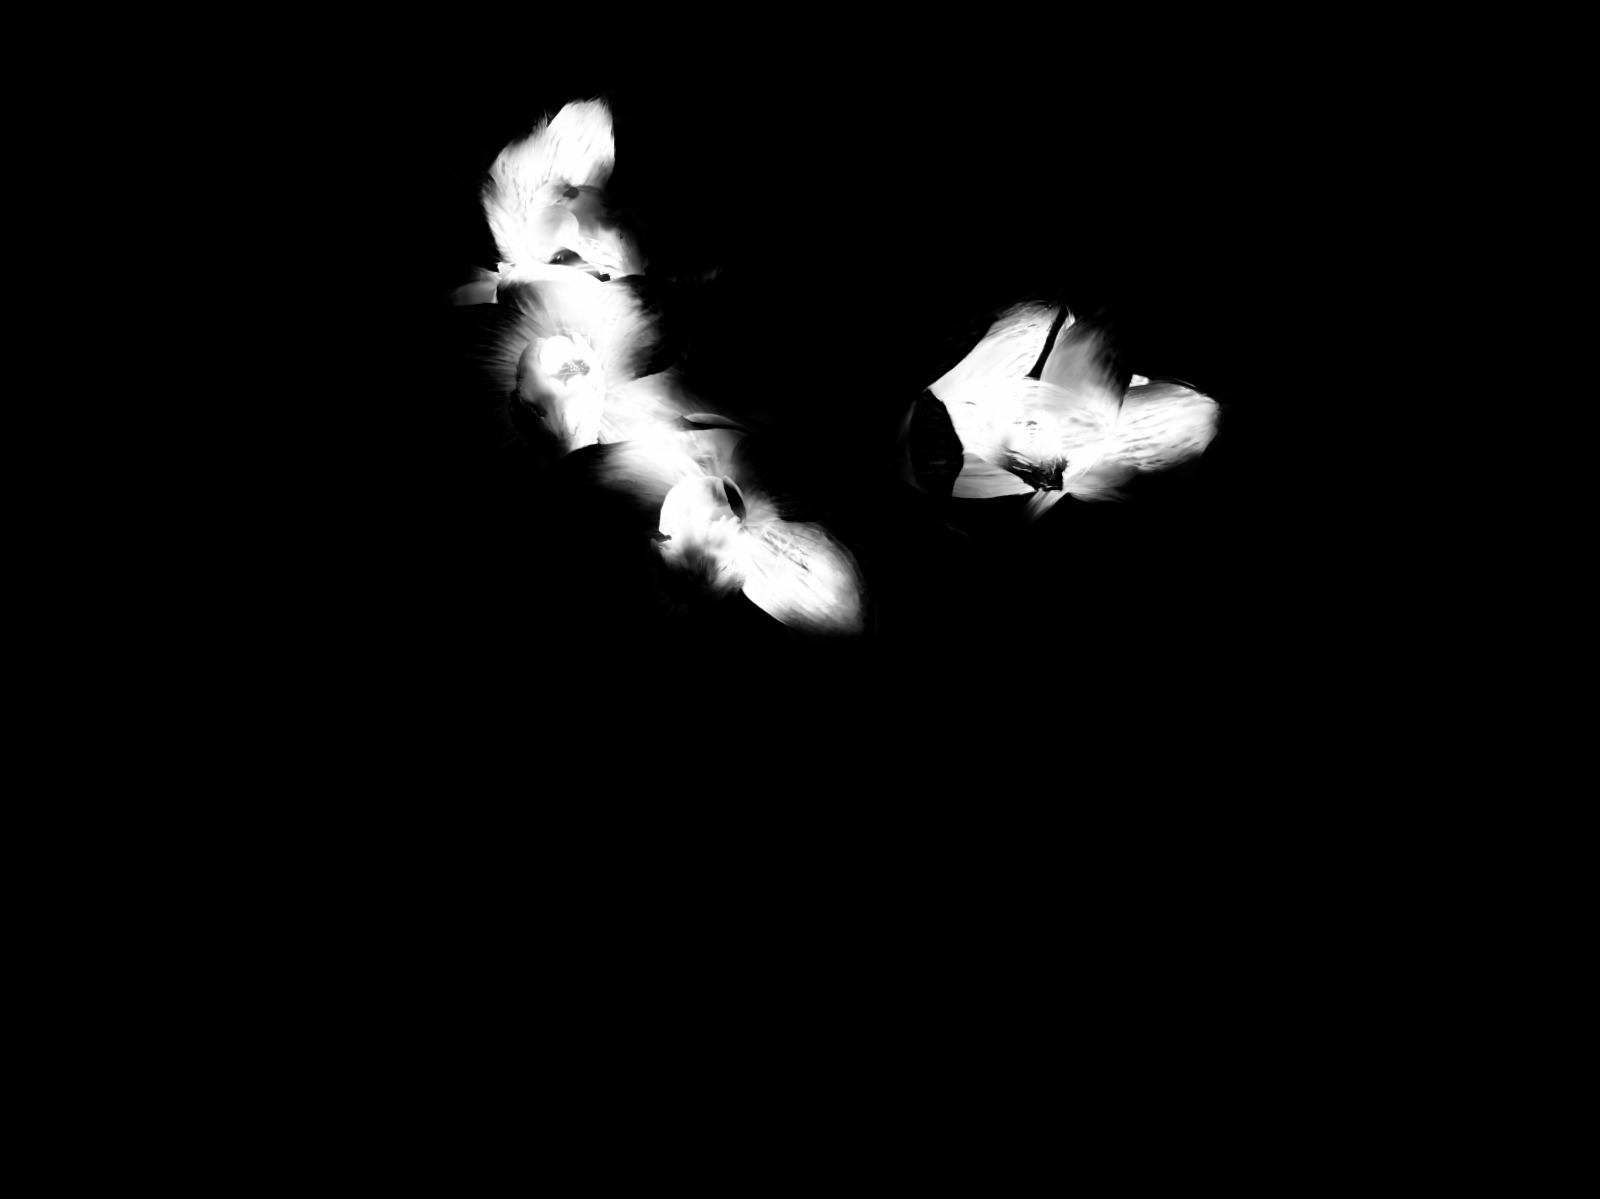
\includegraphics[width=0.2\linewidth]{figures/diffusion_appendix/orchids_sim_3it.jpg}
    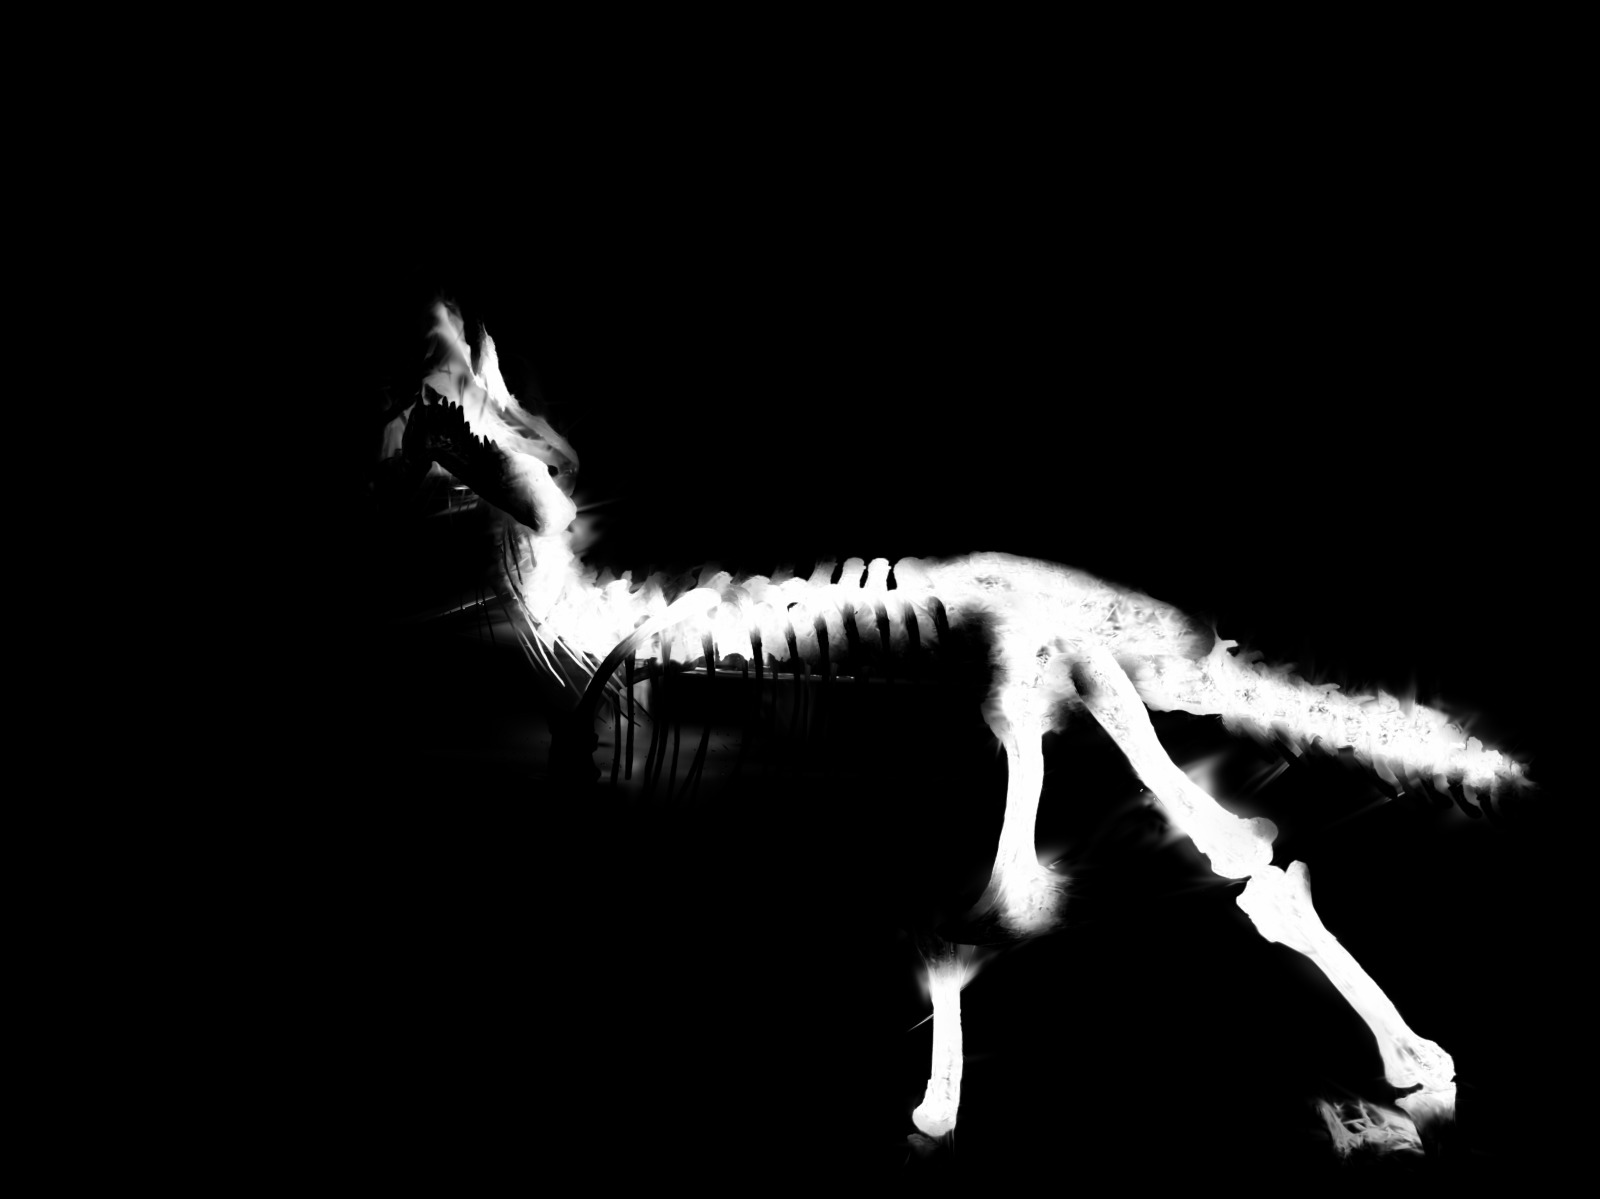
\includegraphics[width=0.2\linewidth]{figures/diffusion_appendix/trex_sim_3it.jpg} \\
    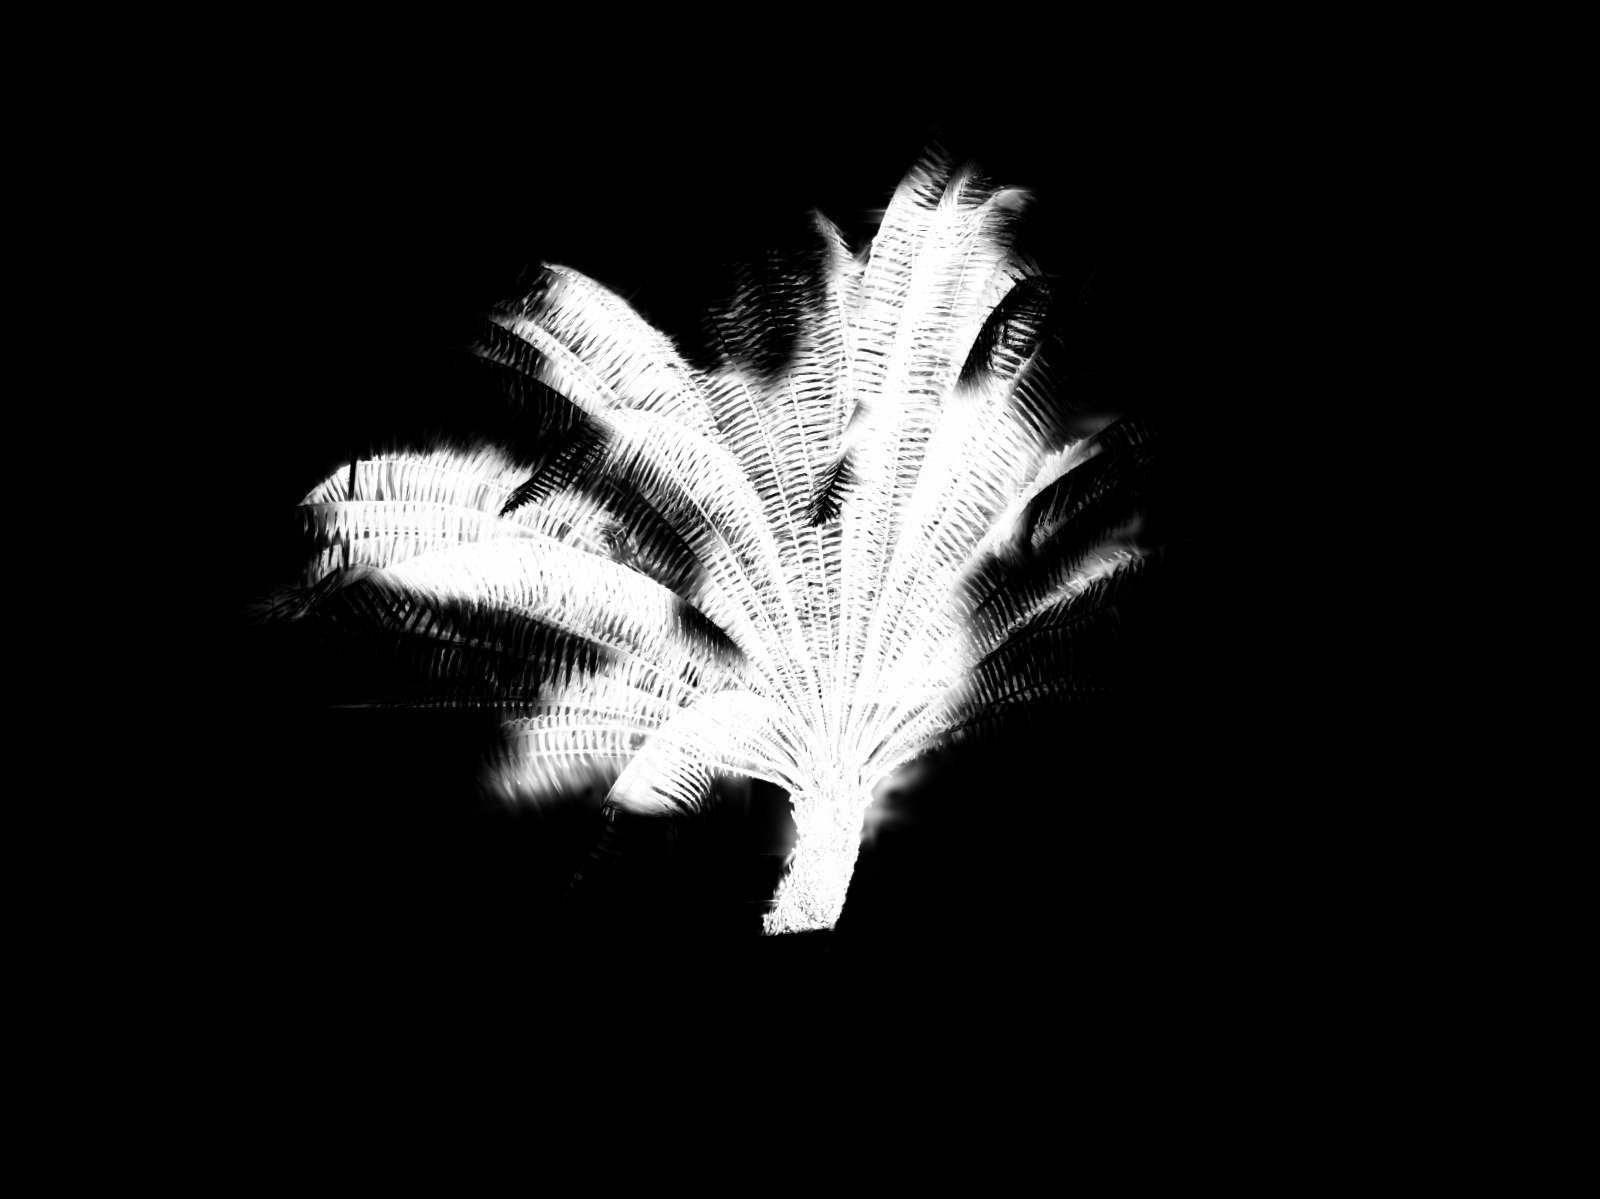
\includegraphics[width=0.2\linewidth]{figures/diffusion_appendix/fern_sim_5it.jpg}
    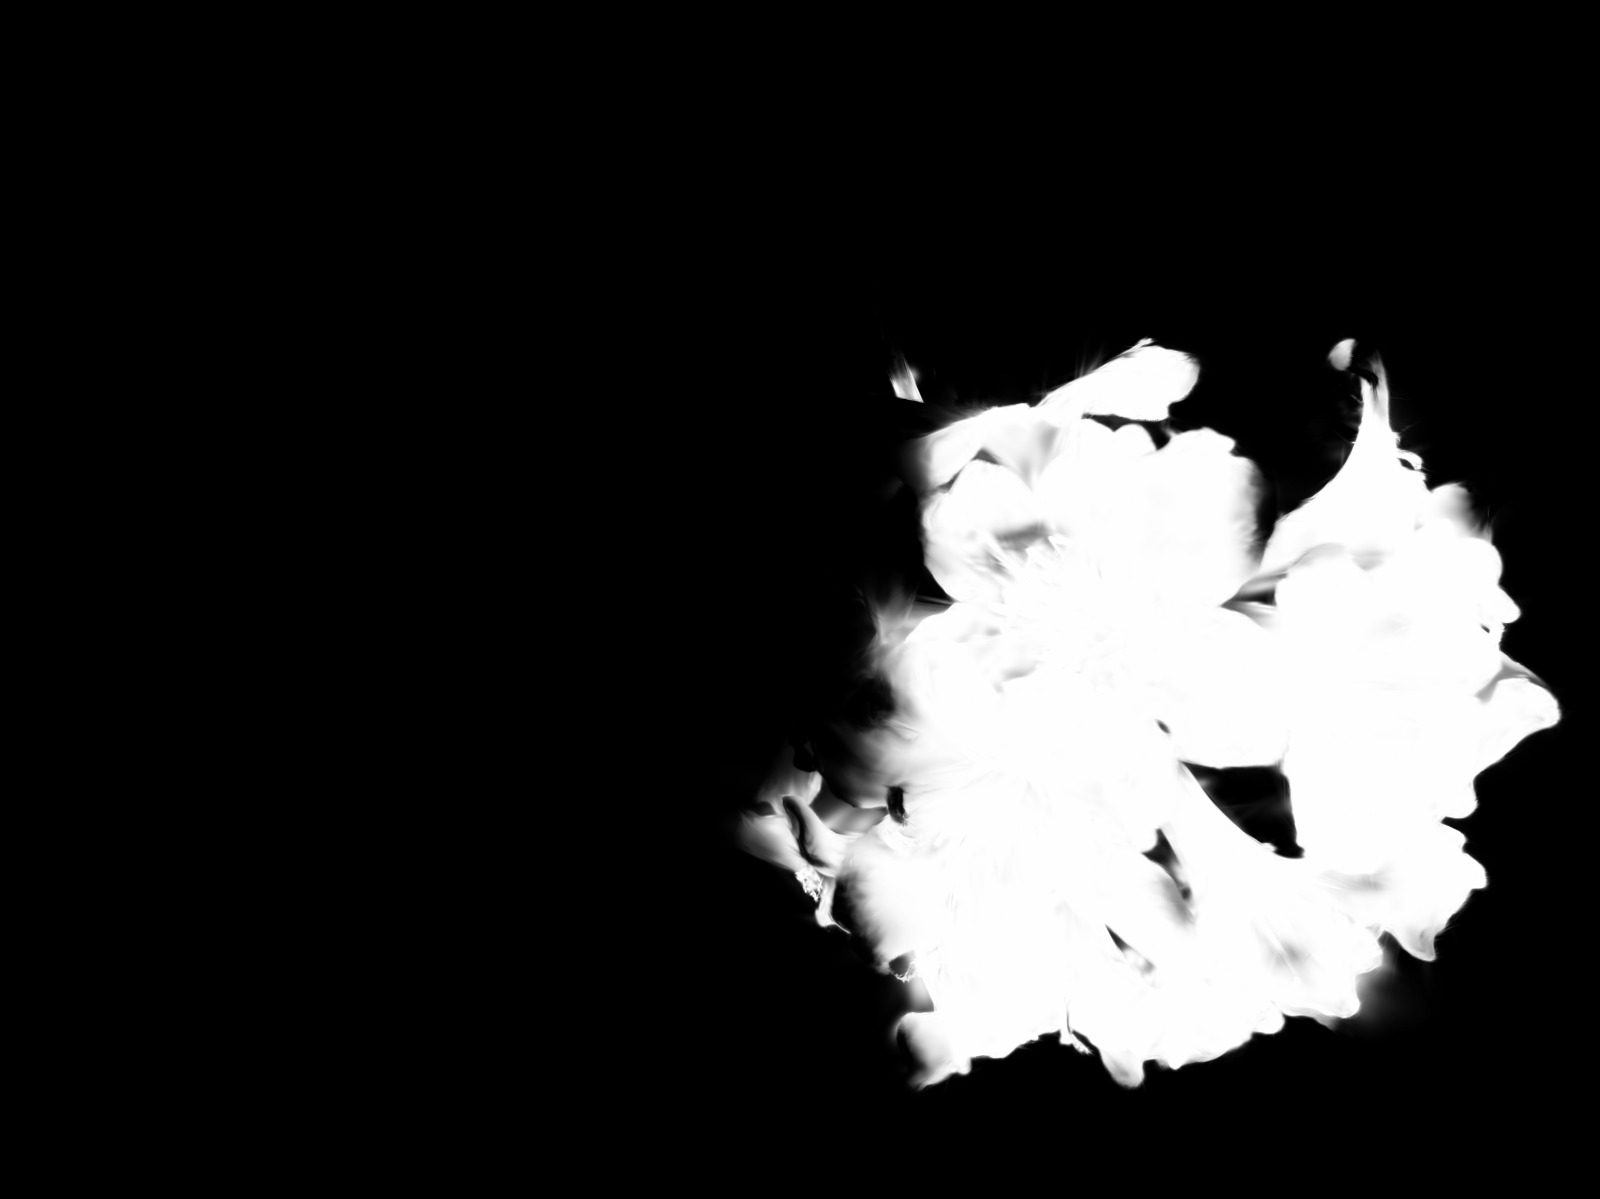
\includegraphics[width=0.2\linewidth]{figures/diffusion_appendix/flower_sim_5it.jpg}
    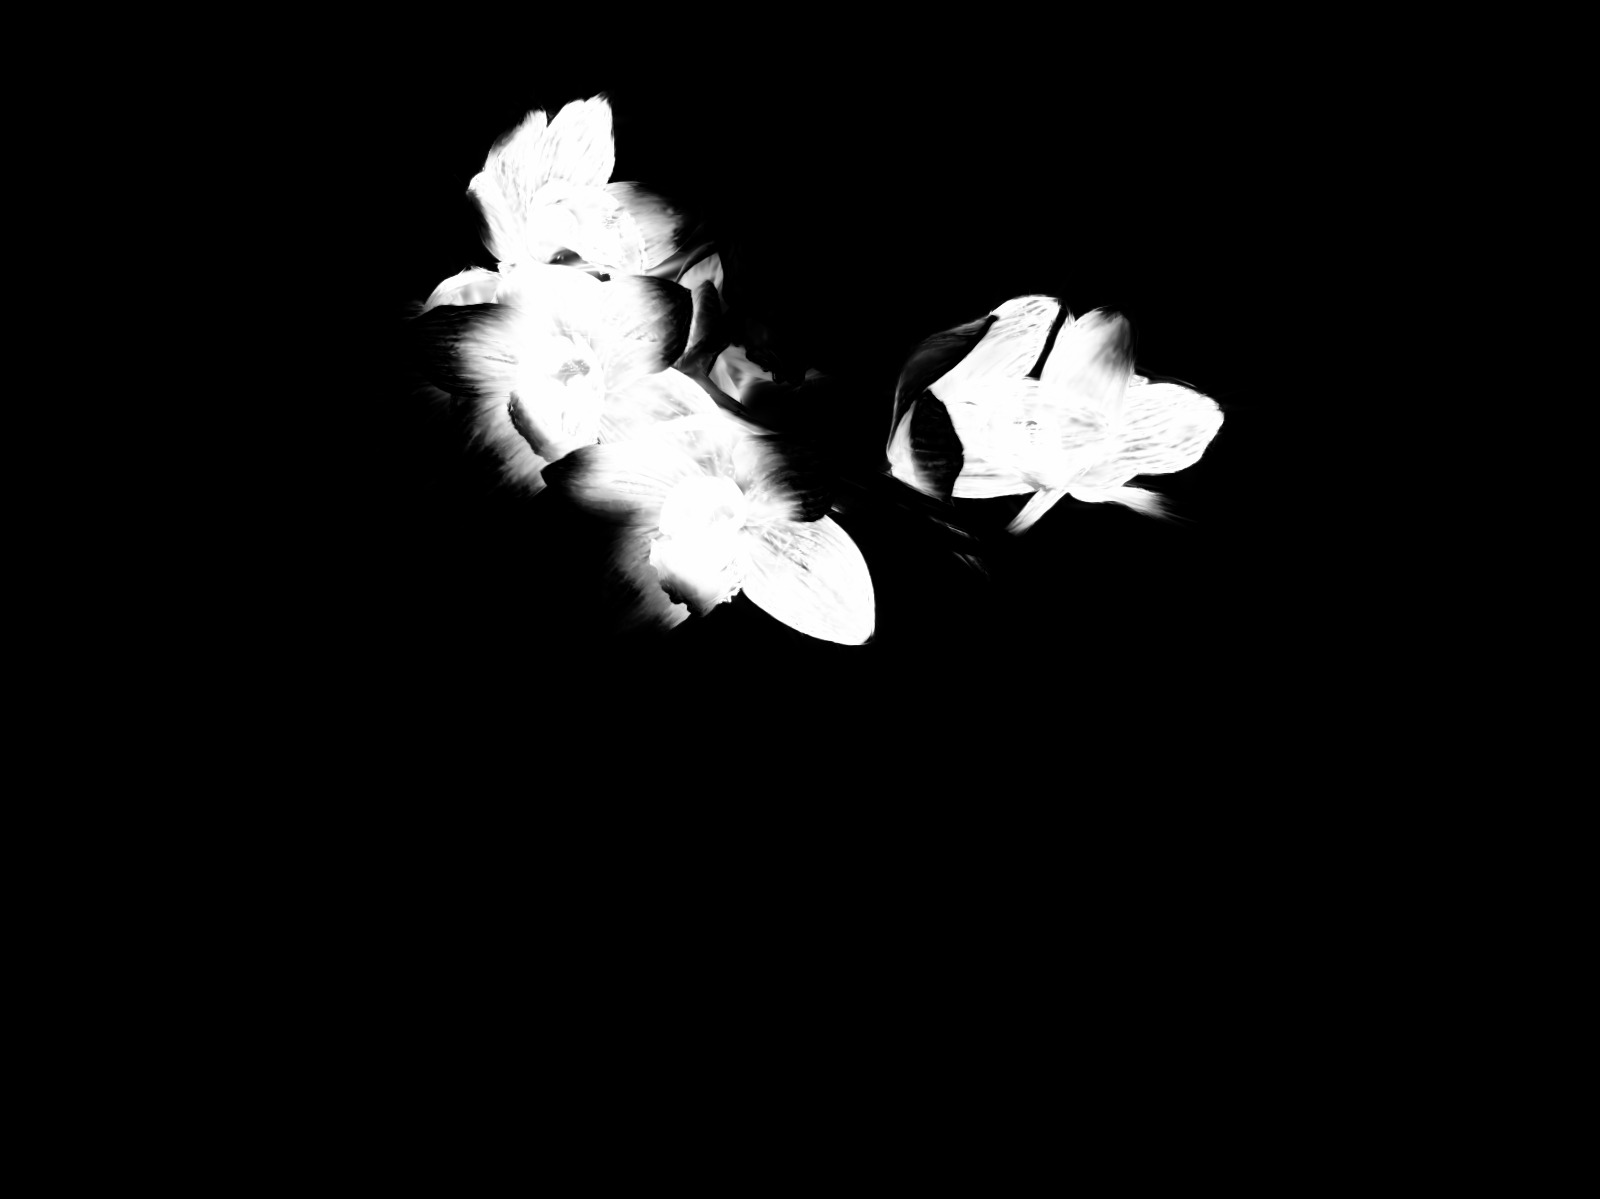
\includegraphics[width=0.2\linewidth]{figures/diffusion_appendix/orchids_sim_5it.jpg}
    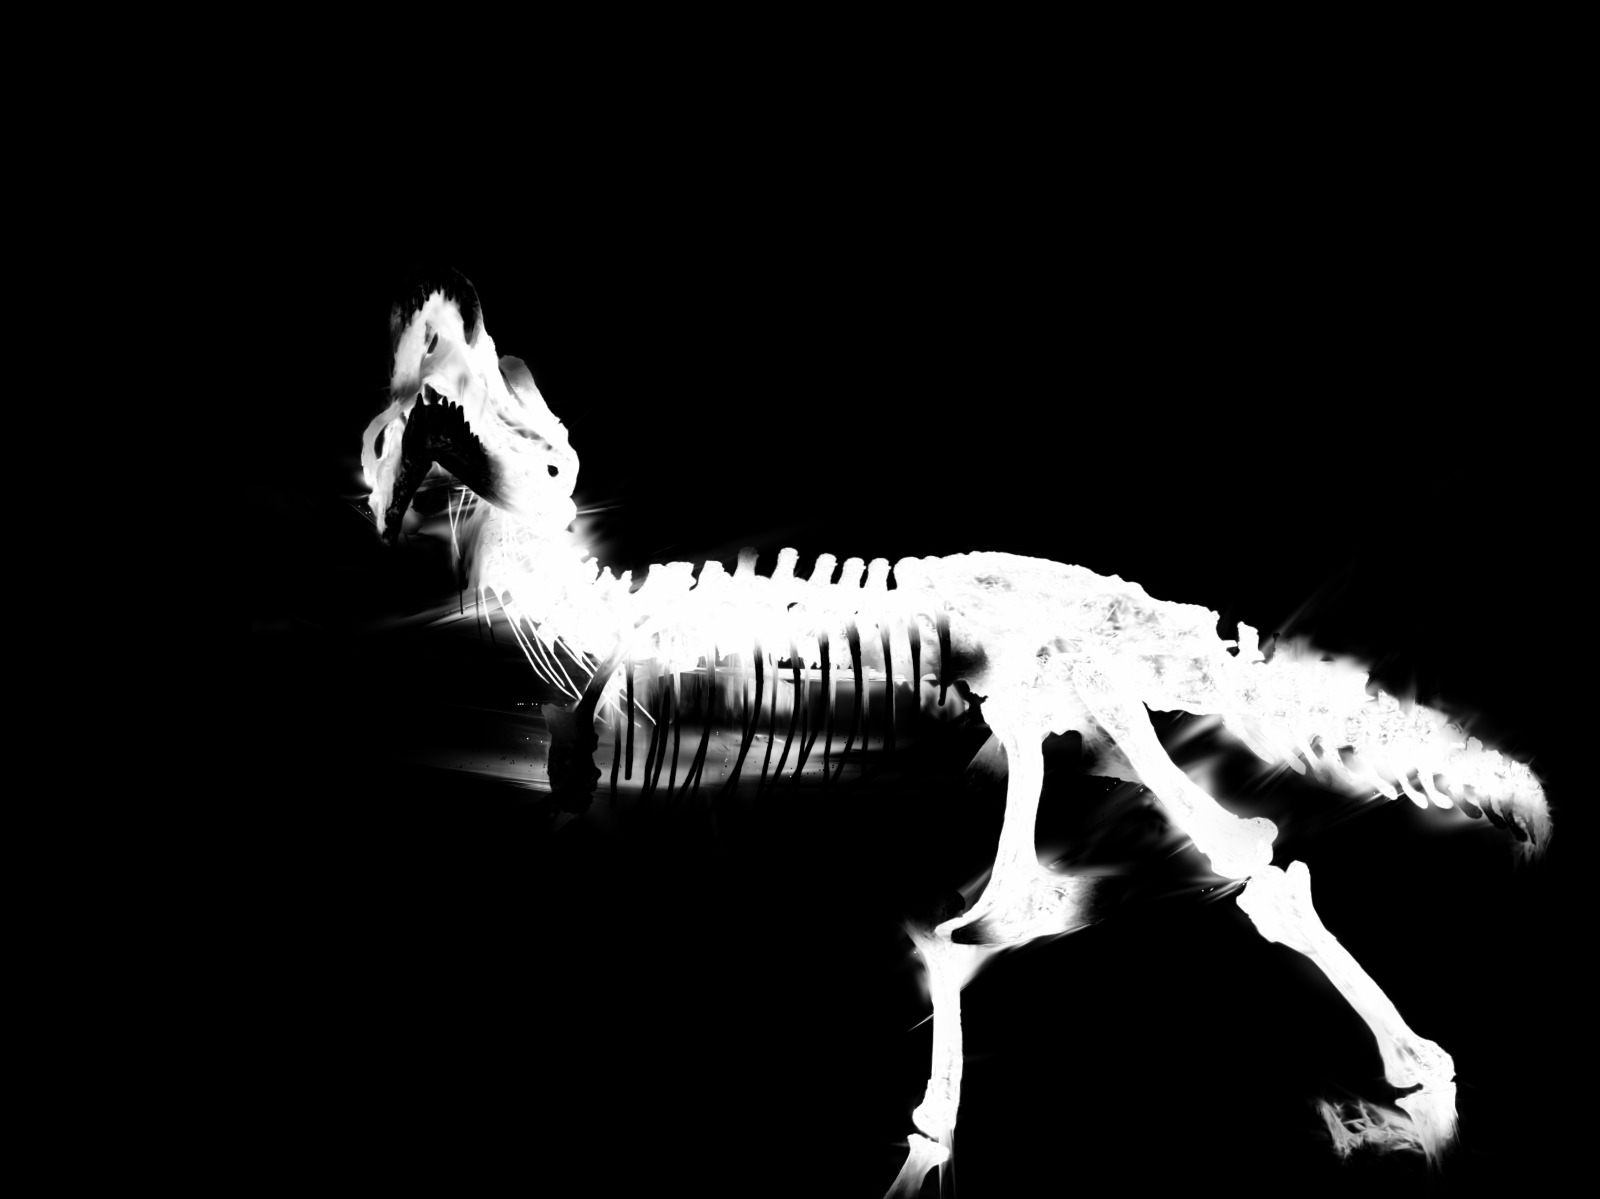
\includegraphics[width=0.2\linewidth]{figures/diffusion_appendix/trex_sim_5it.jpg} \\
    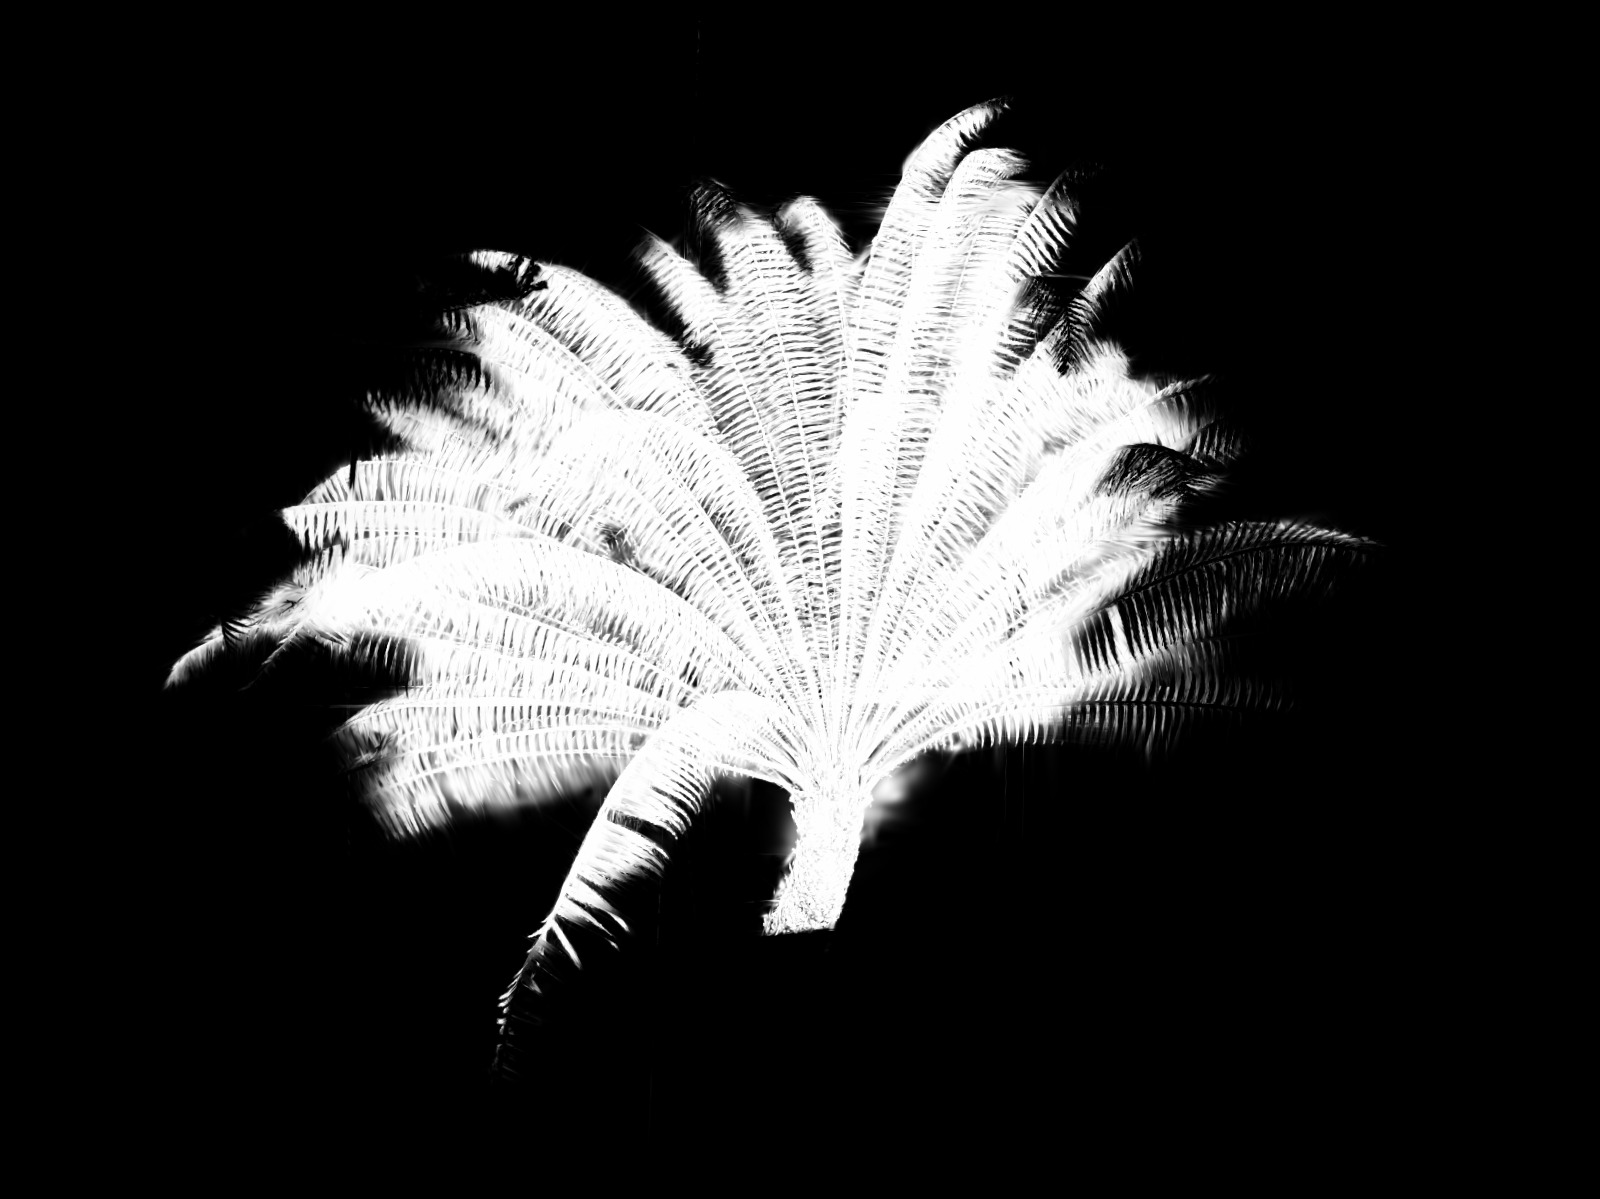
\includegraphics[width=0.2\linewidth]{figures/diffusion_appendix/fern_sim_10it.jpg}
    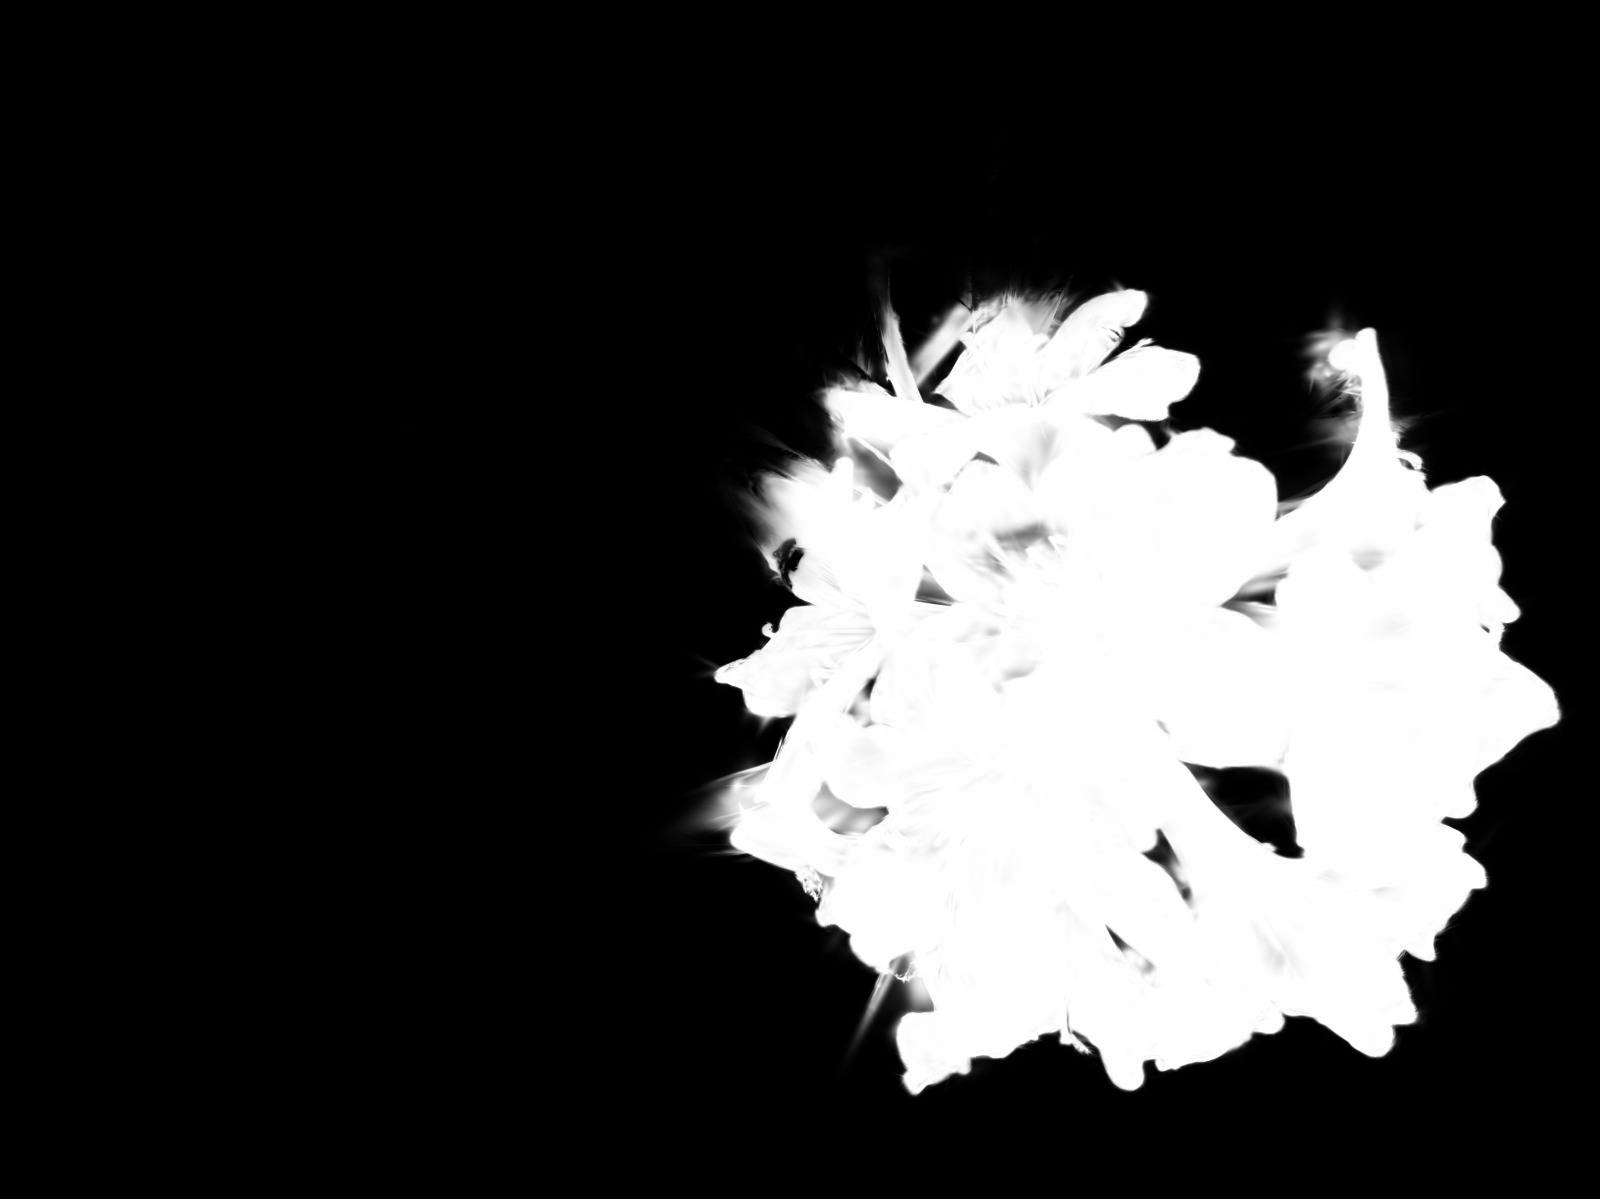
\includegraphics[width=0.2\linewidth]{figures/diffusion_appendix/flower_sim_10it.jpg}
    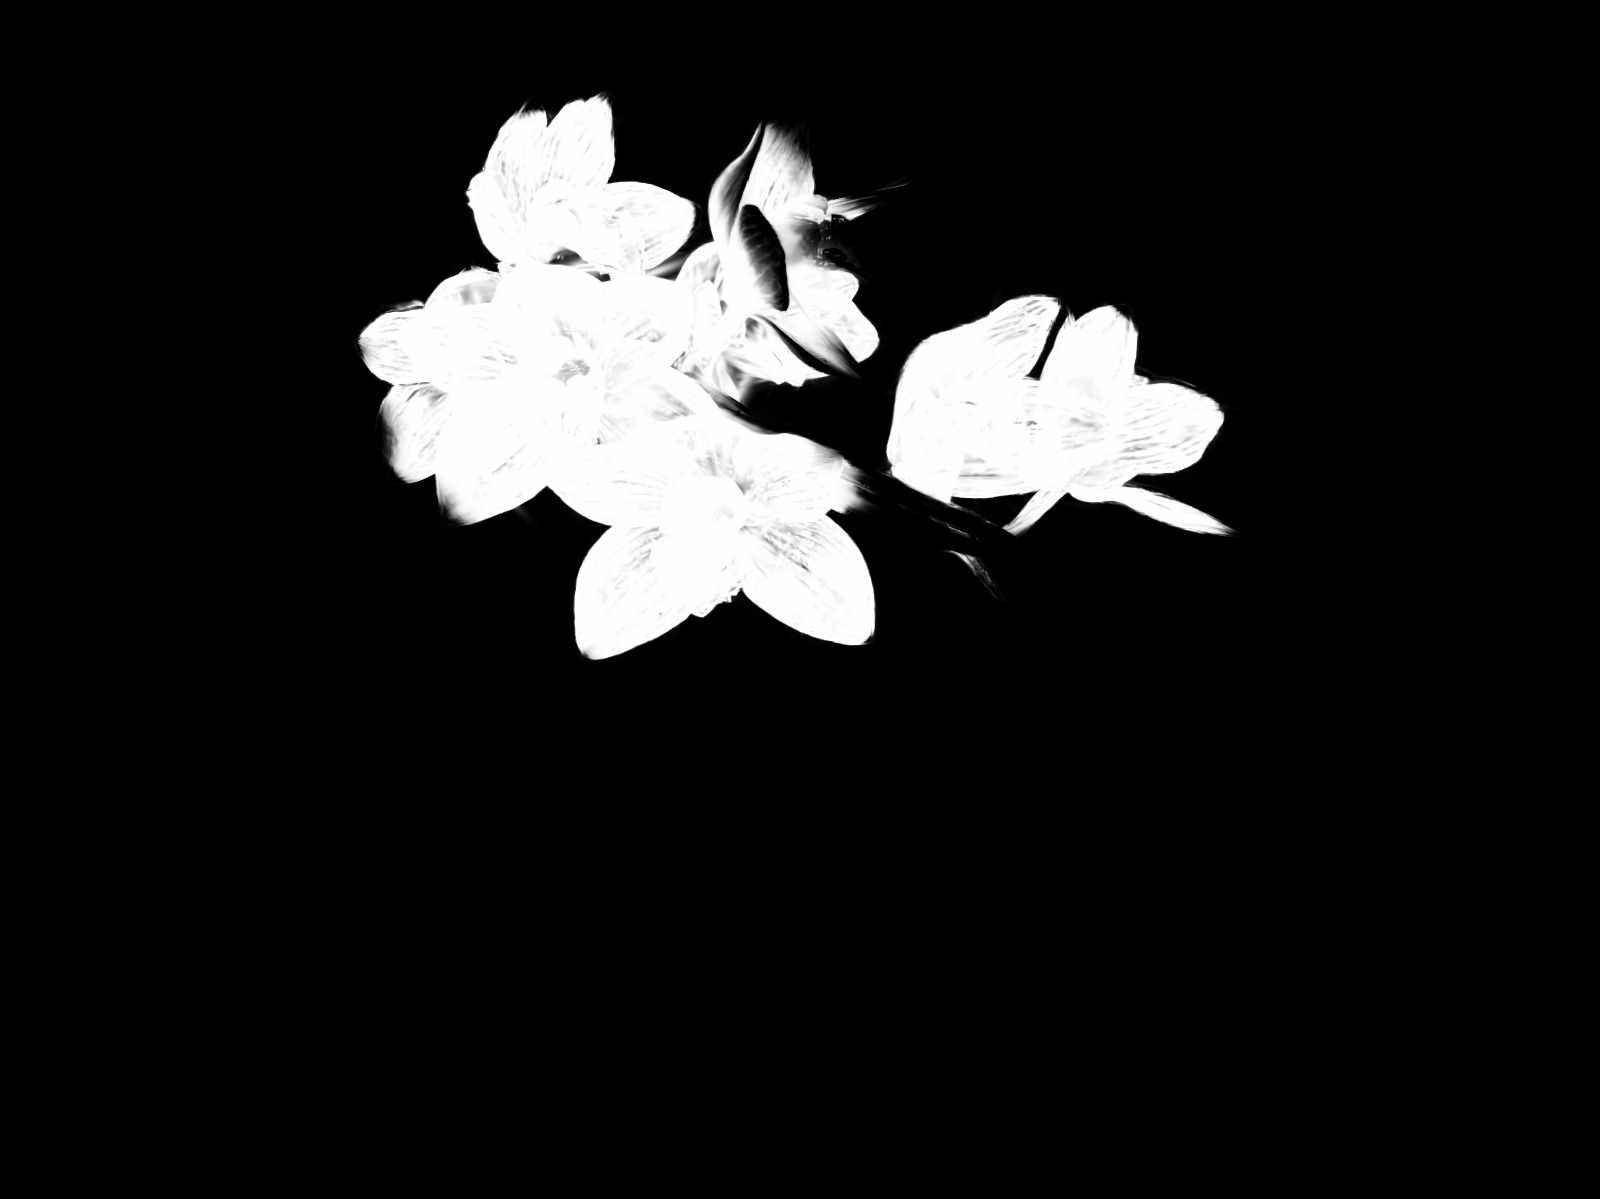
\includegraphics[width=0.2\linewidth]{figures/diffusion_appendix/orchids_sim_10it.jpg}
    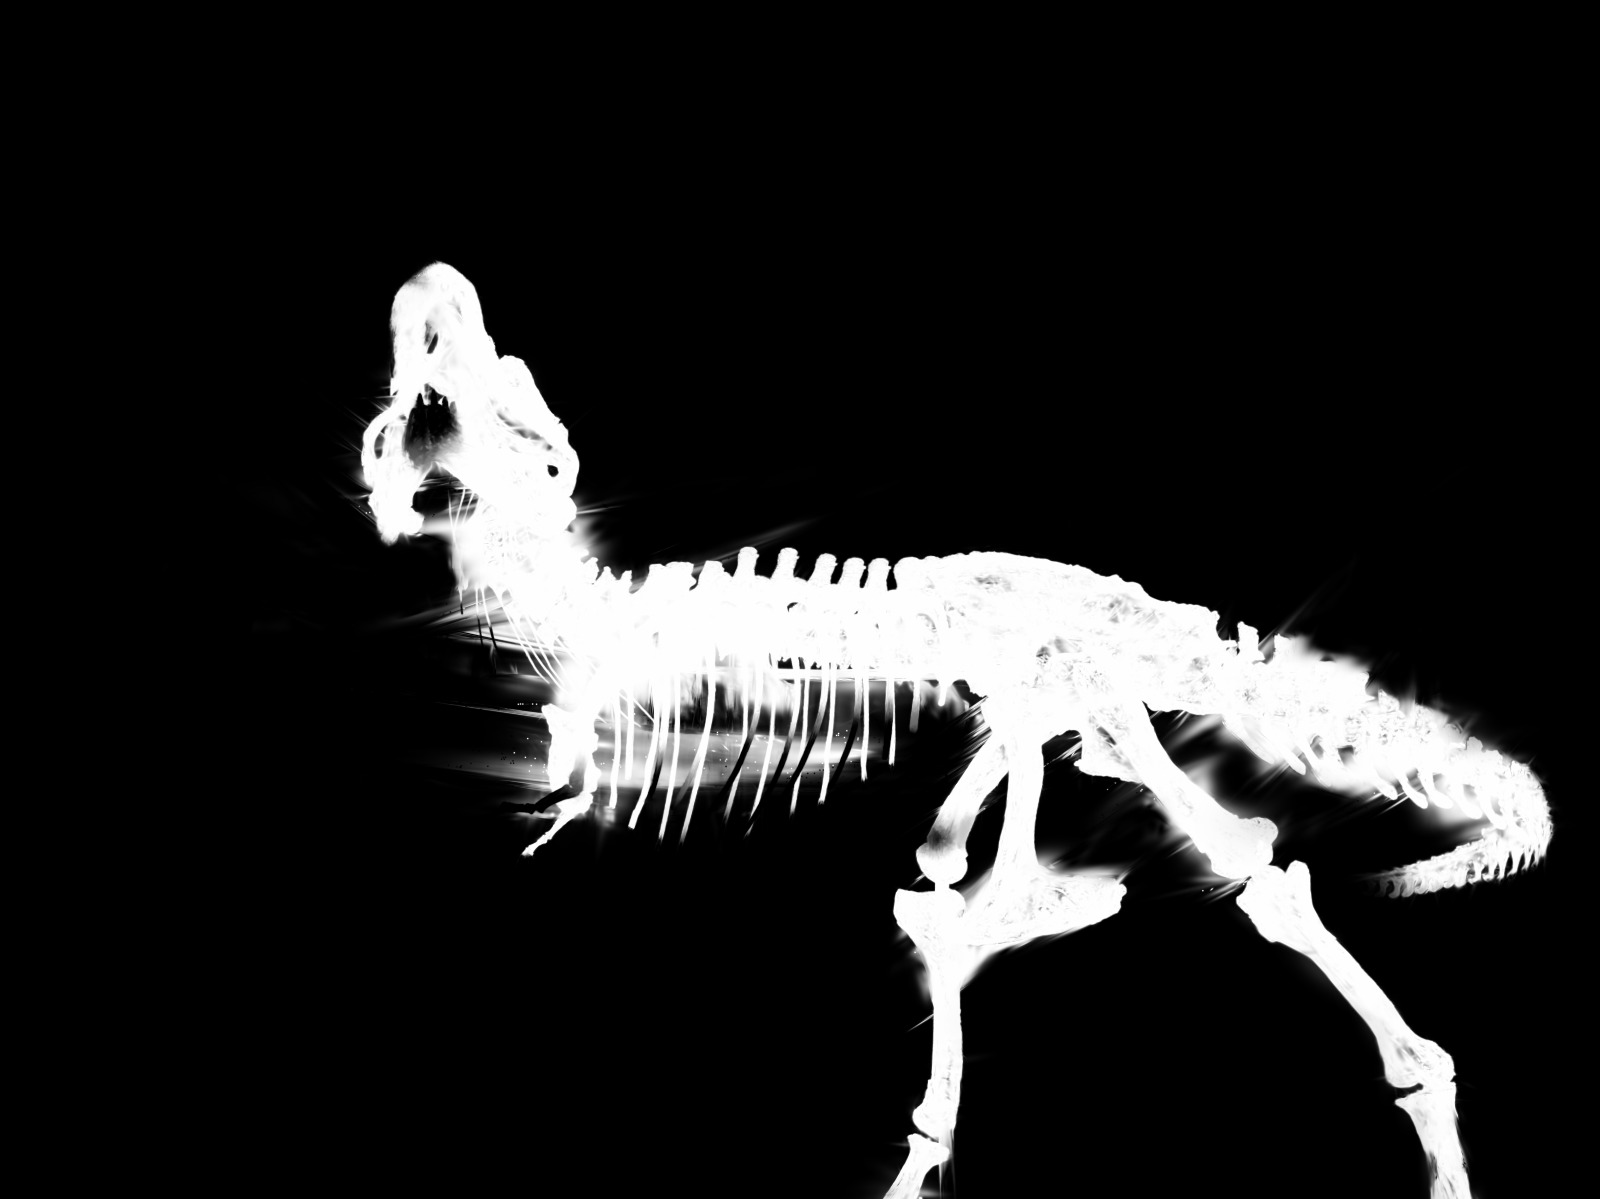
\includegraphics[width=0.2\linewidth]{figures/diffusion_appendix/trex_sim_10it.jpg} \\
    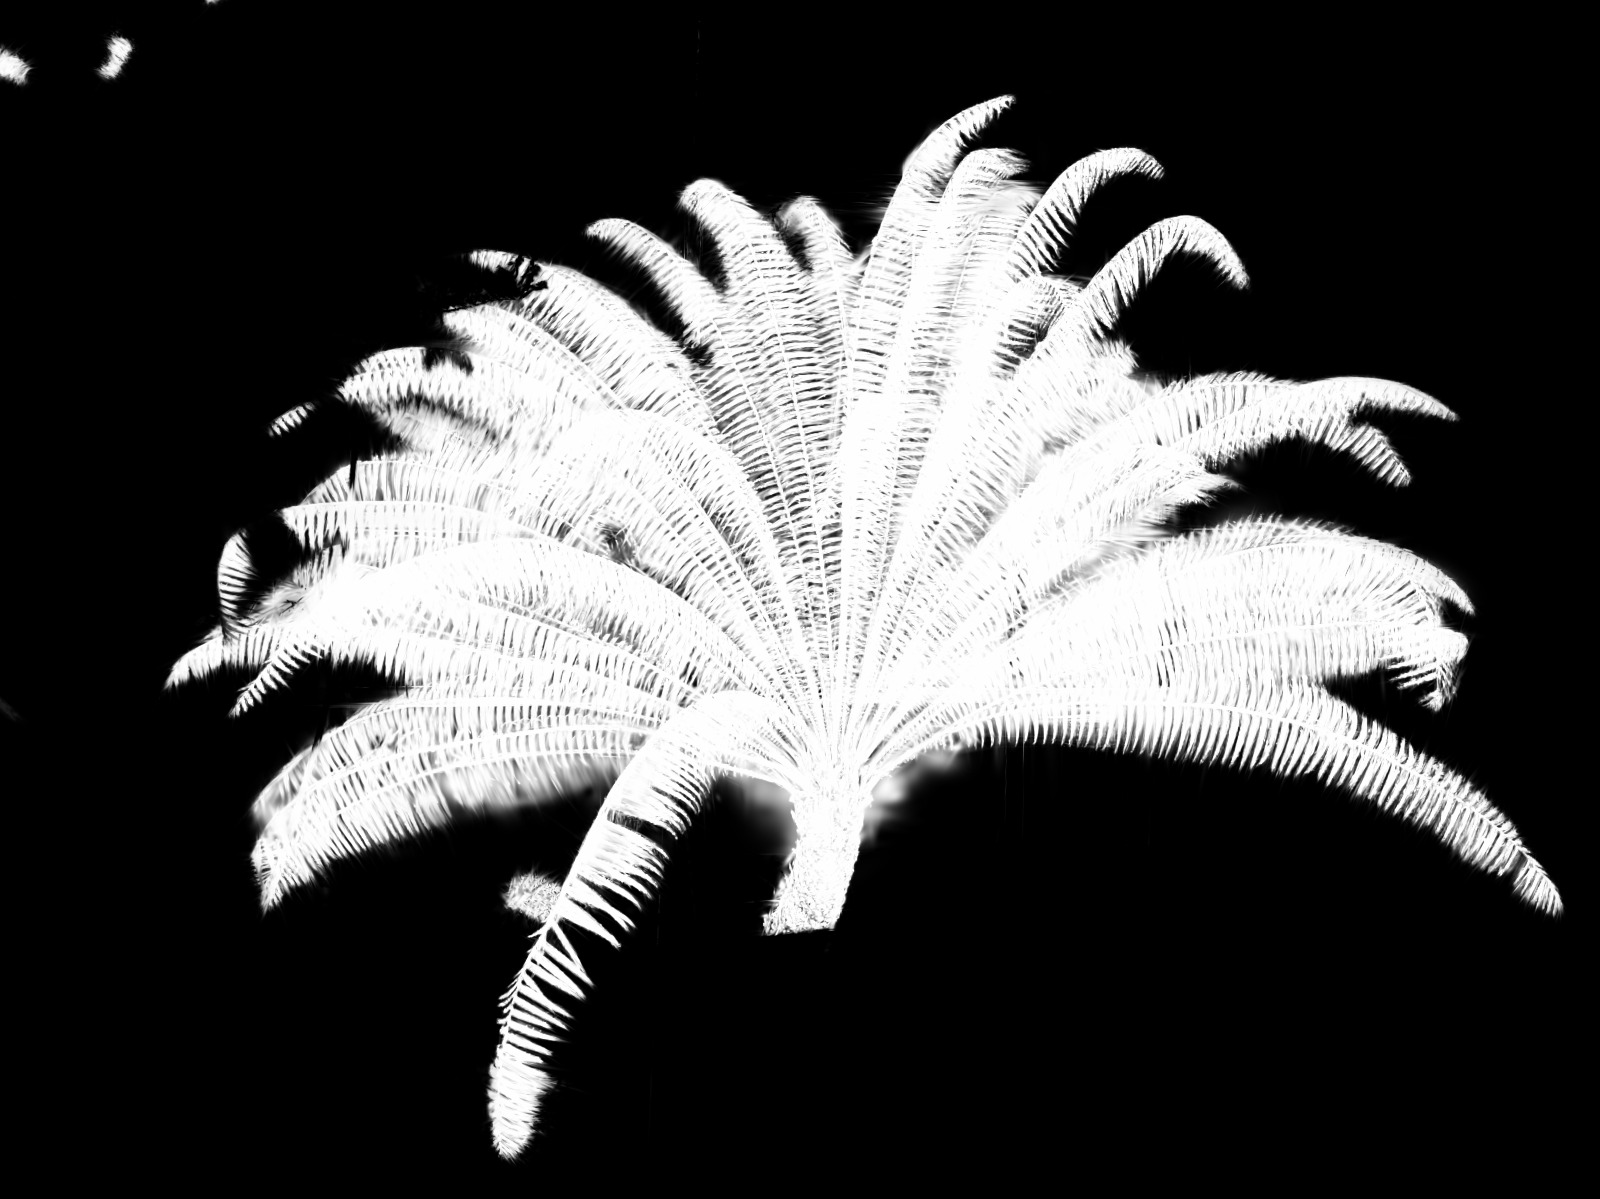
\includegraphics[width=0.2\linewidth]{figures/diffusion_appendix/fern_sim.jpg}
    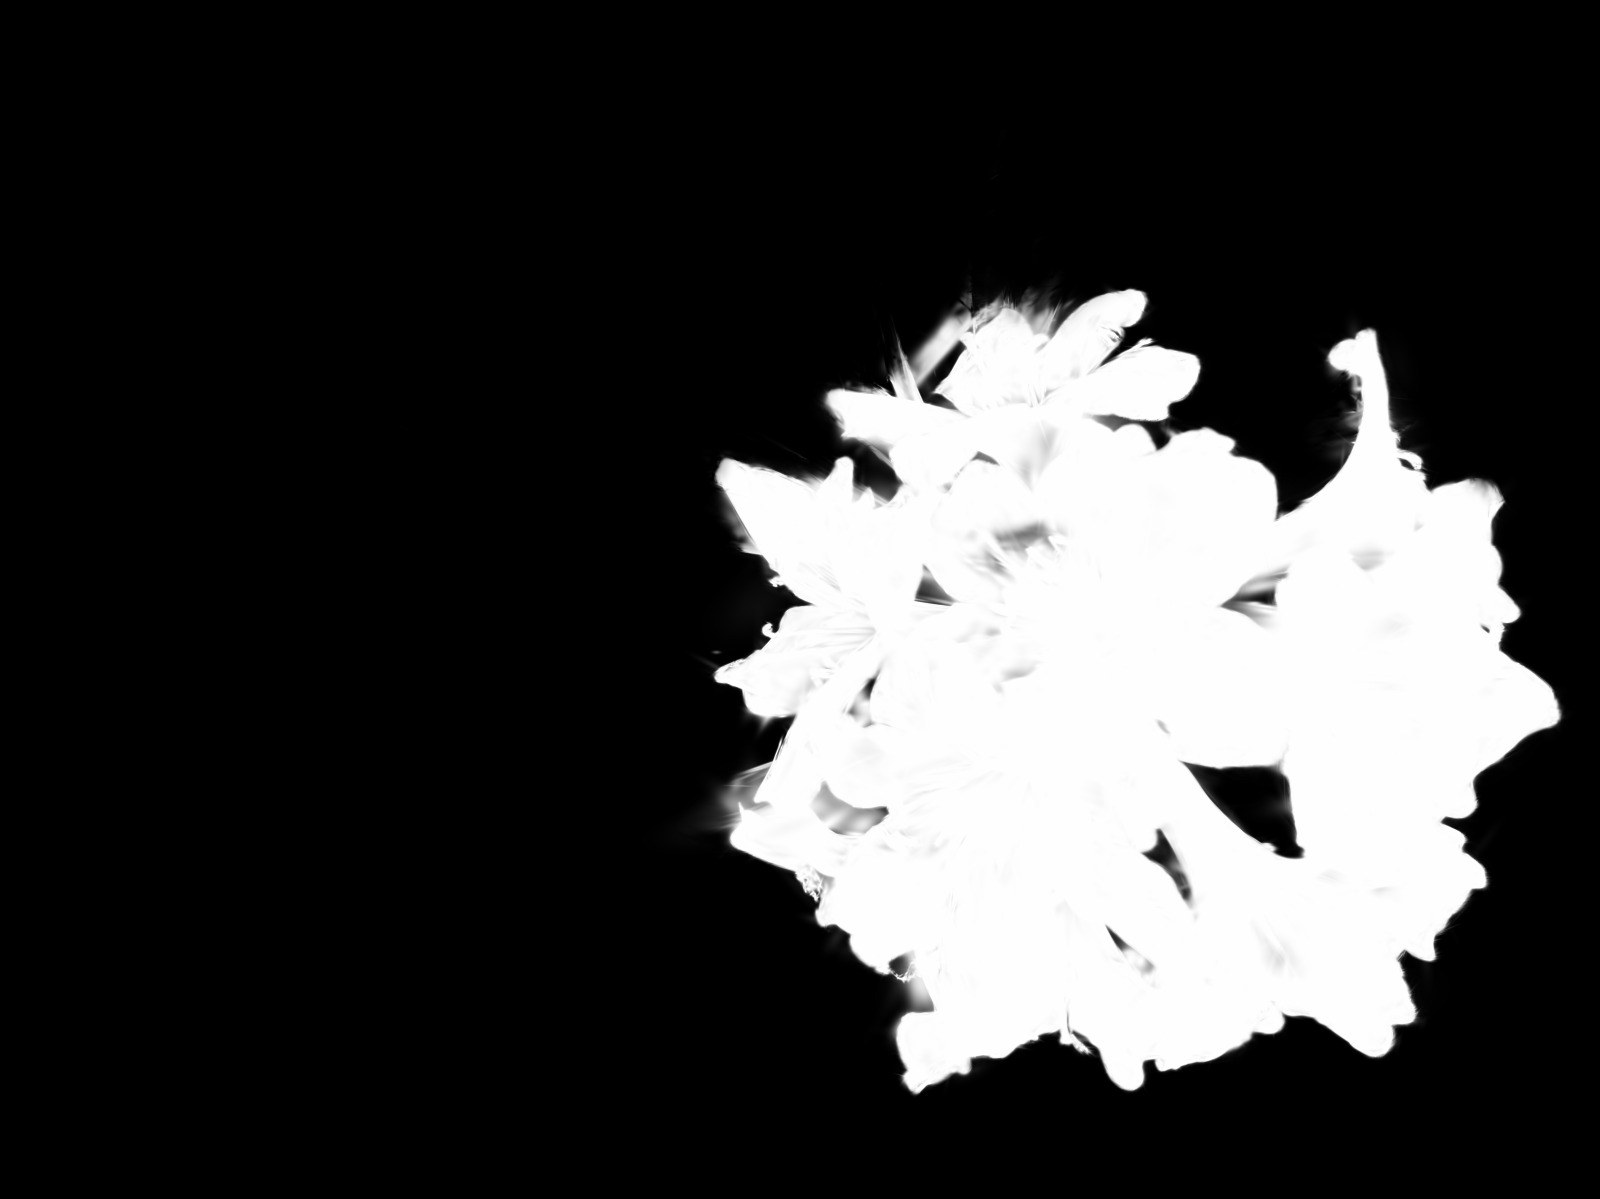
\includegraphics[width=0.2\linewidth]{figures/diffusion_appendix/flower_sim.jpg}
    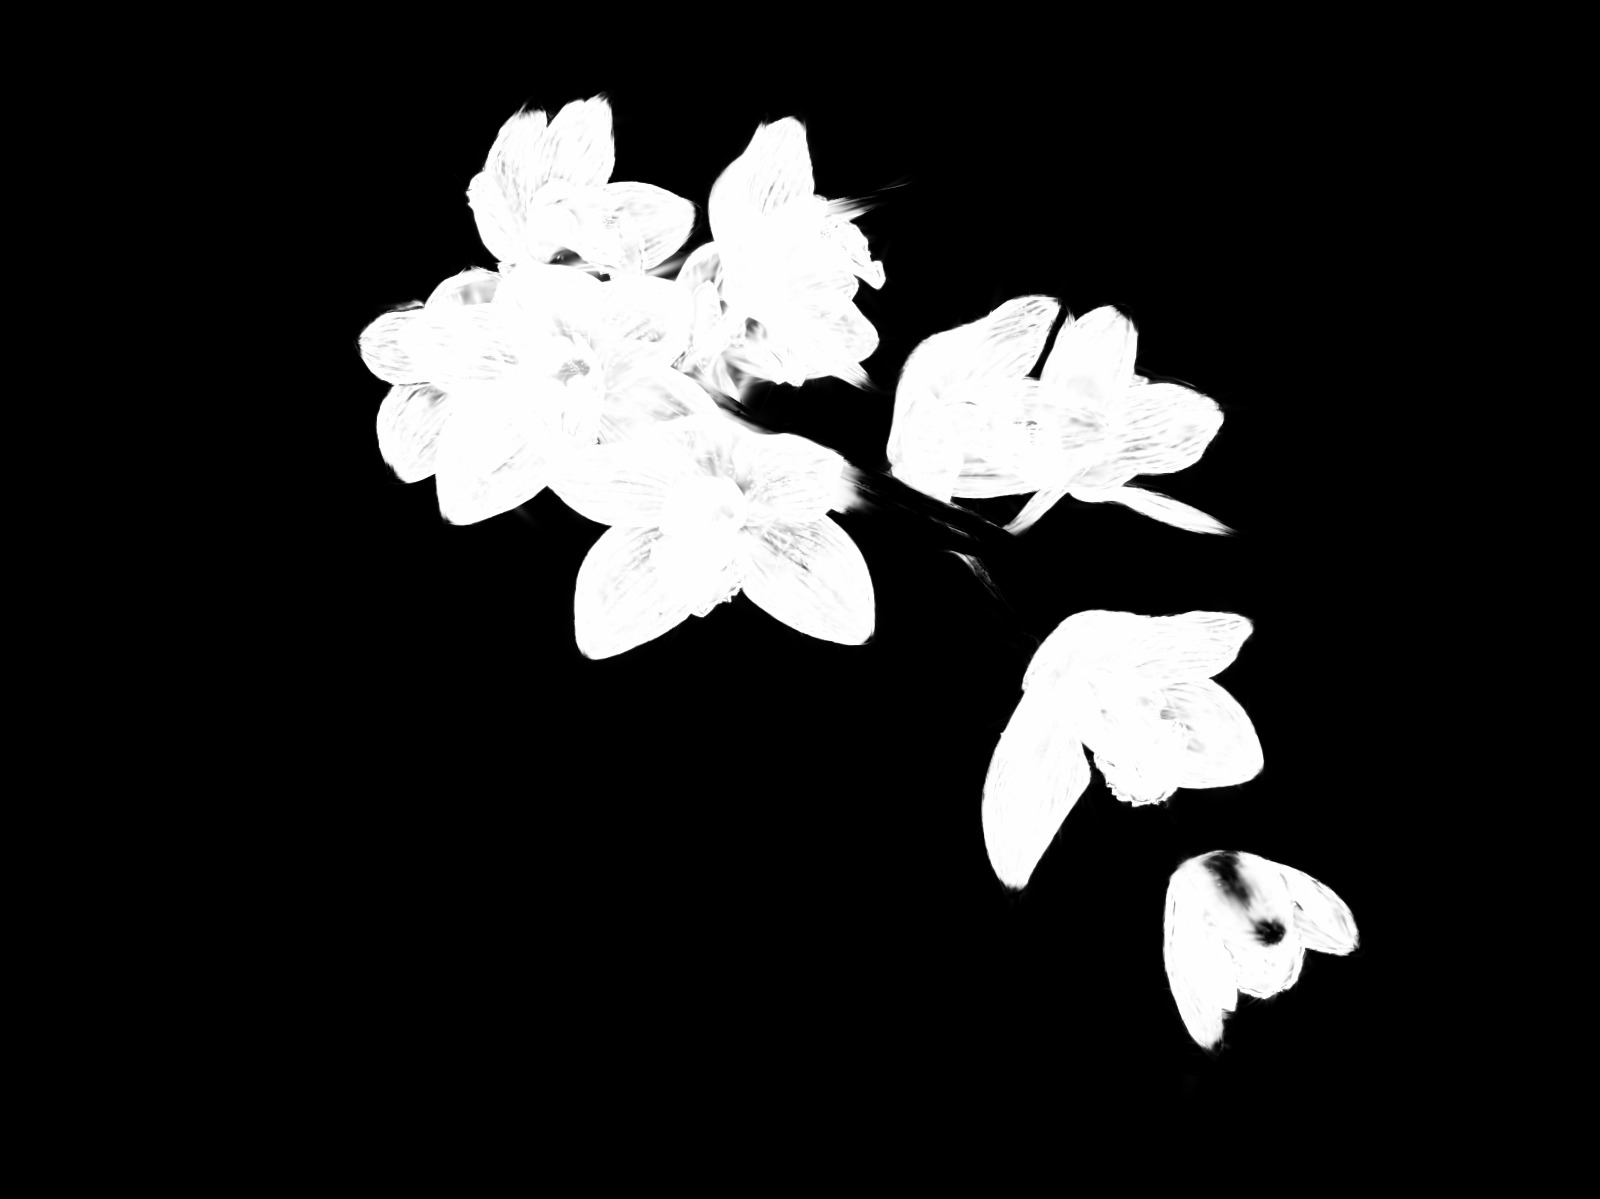
\includegraphics[width=0.2\linewidth]{figures/diffusion_appendix/orchids_sim.jpg}
    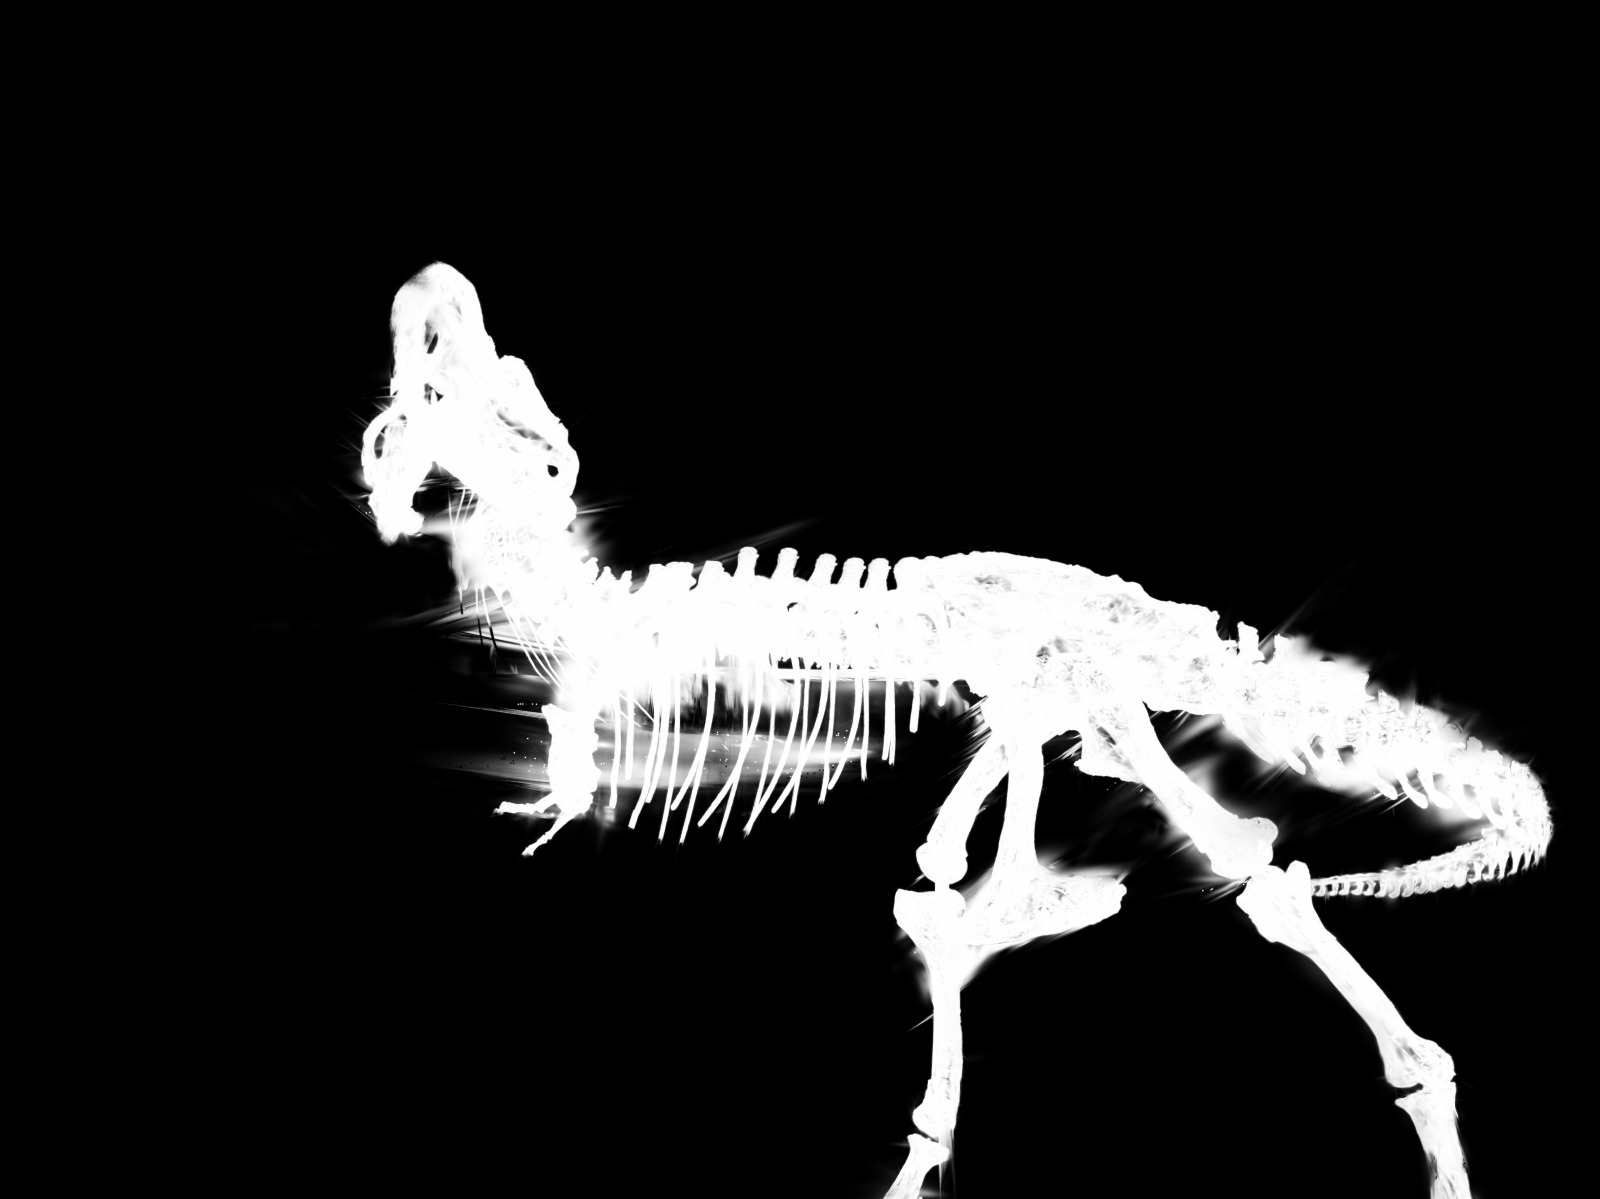
\includegraphics[width=0.2\linewidth]{figures/diffusion_appendix/trex_sim.jpg} \\
    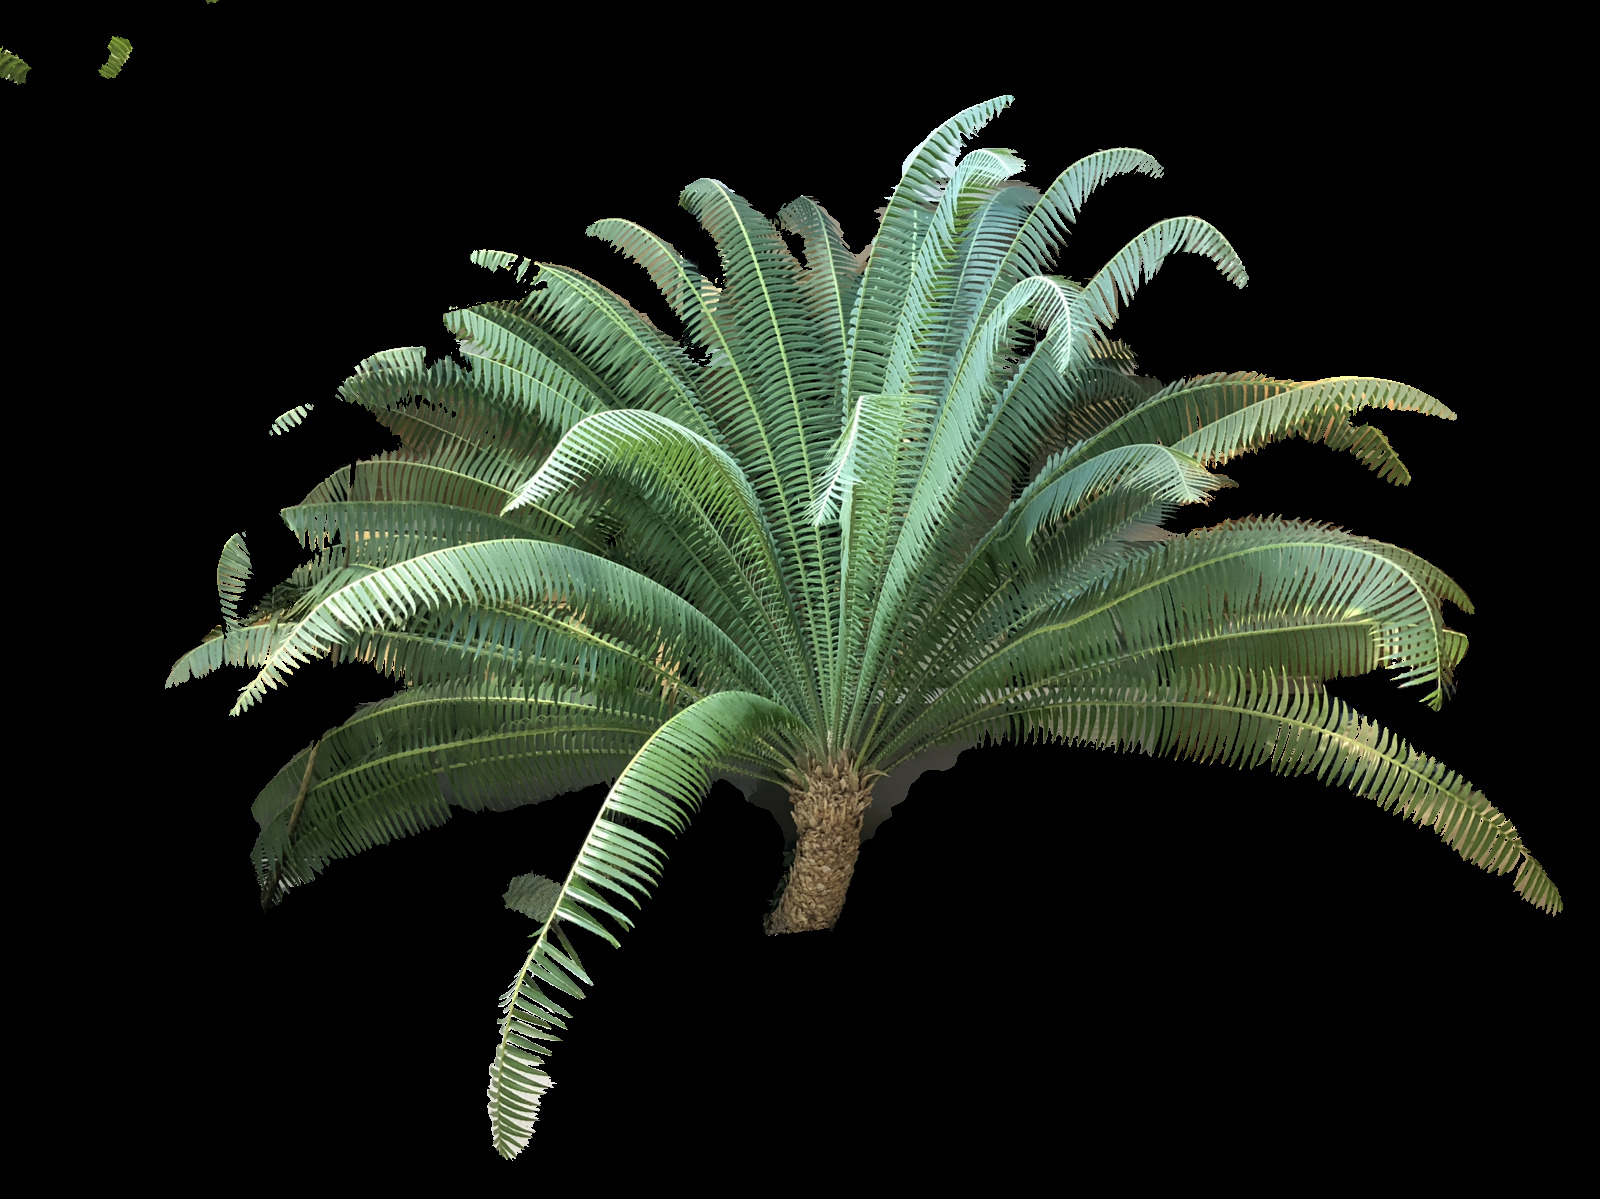
\includegraphics[width=0.2\linewidth]{figures/diffusion_appendix/fern_pred.jpg}
    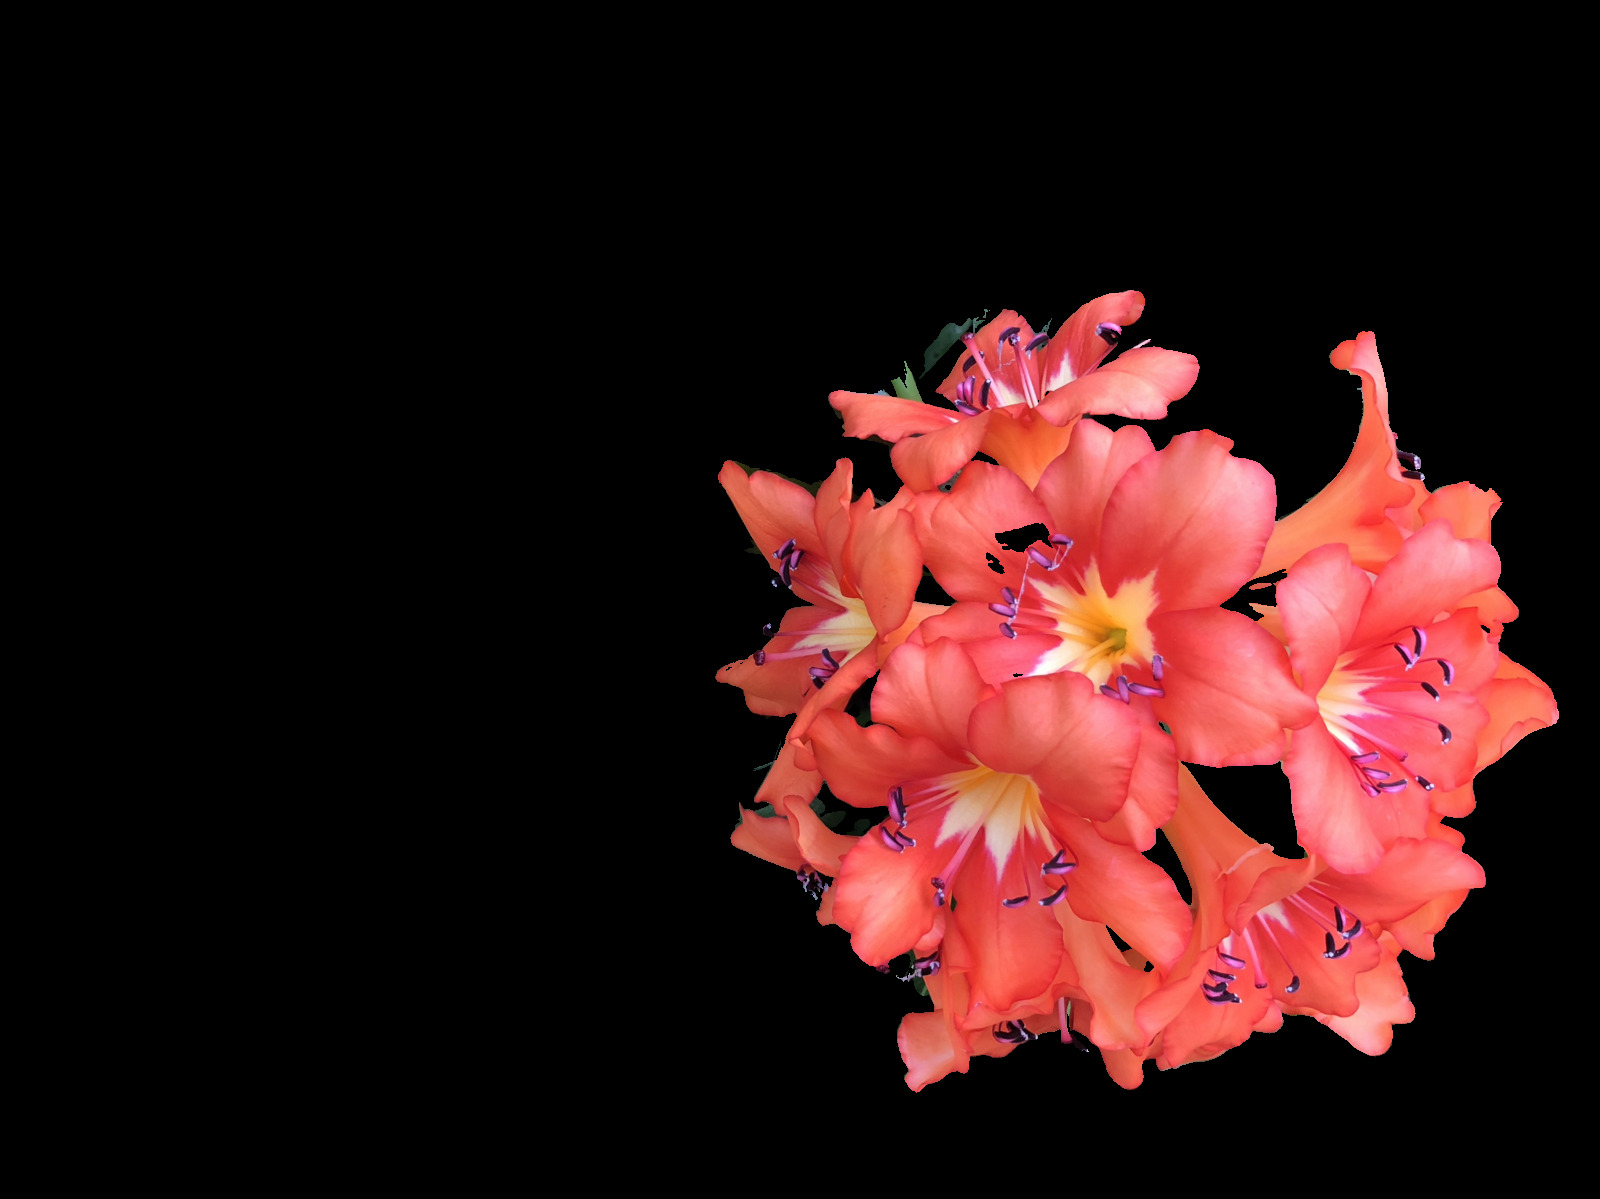
\includegraphics[width=0.2\linewidth]{figures/diffusion_appendix/flower_pred.jpg}
    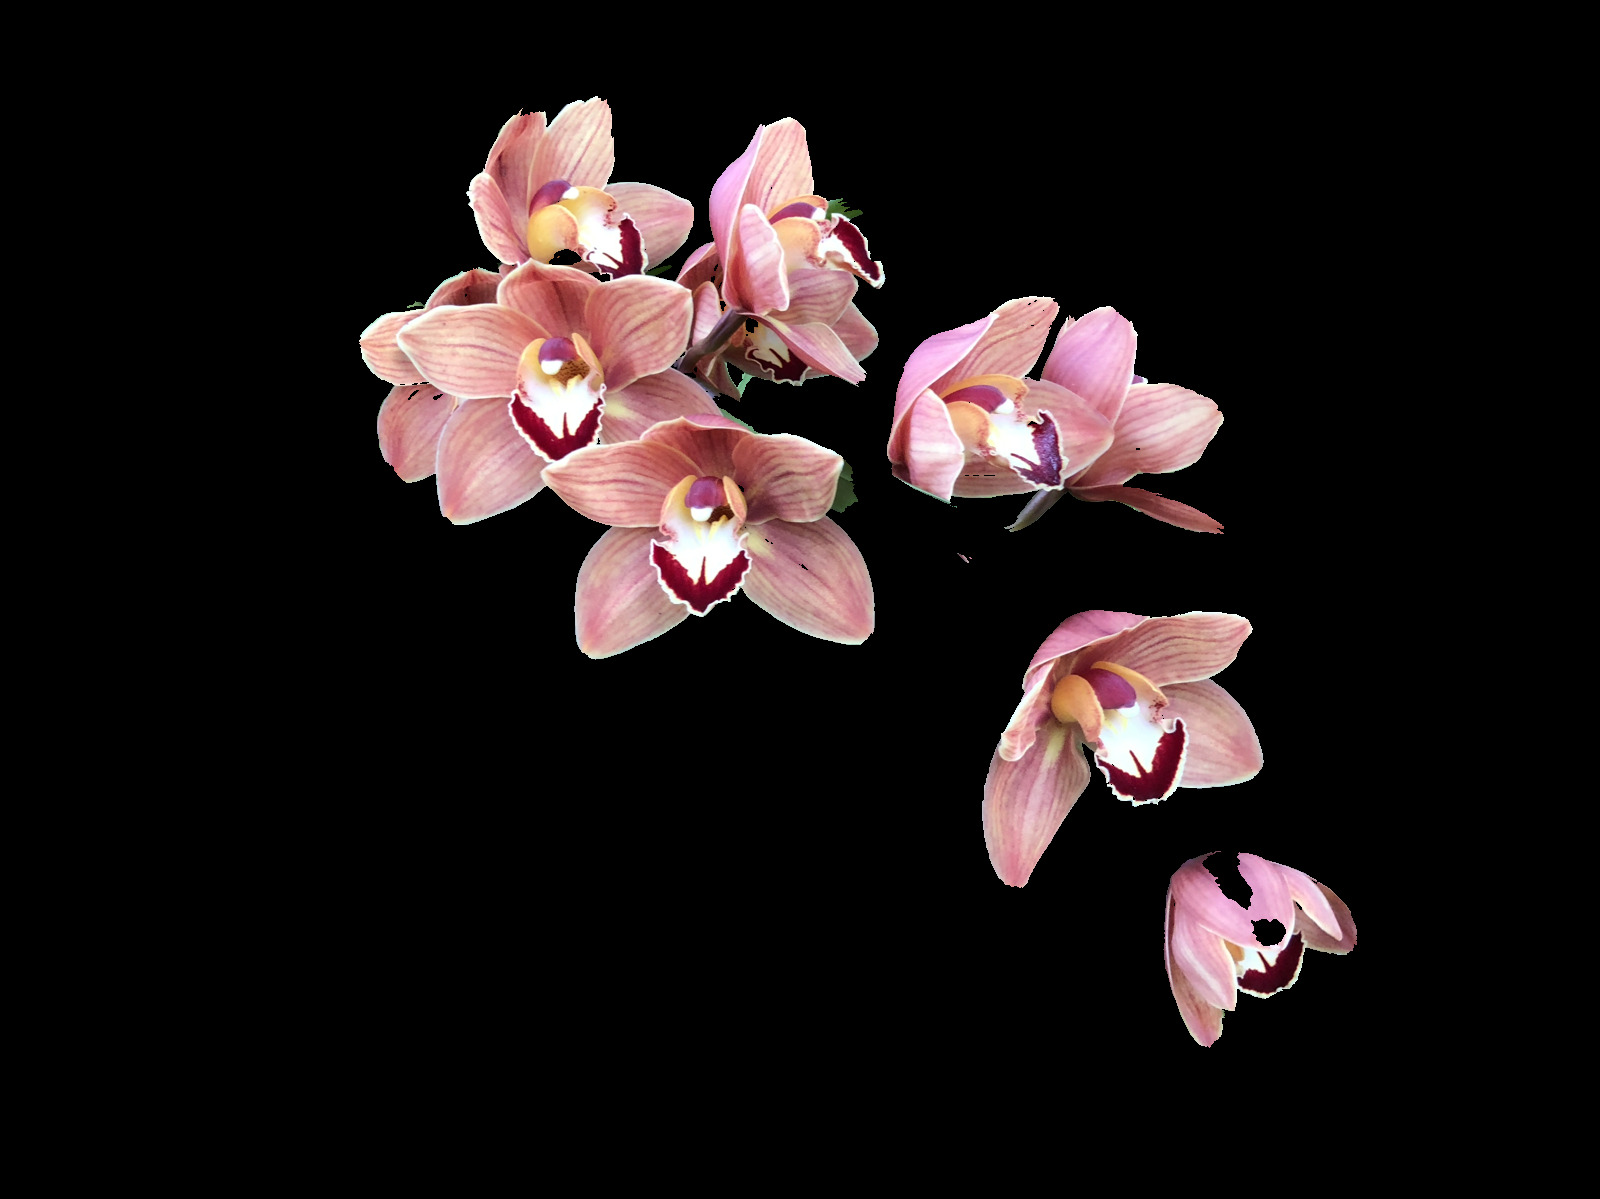
\includegraphics[width=0.2\linewidth]{figures/diffusion_appendix/orchids_pred.jpg}
    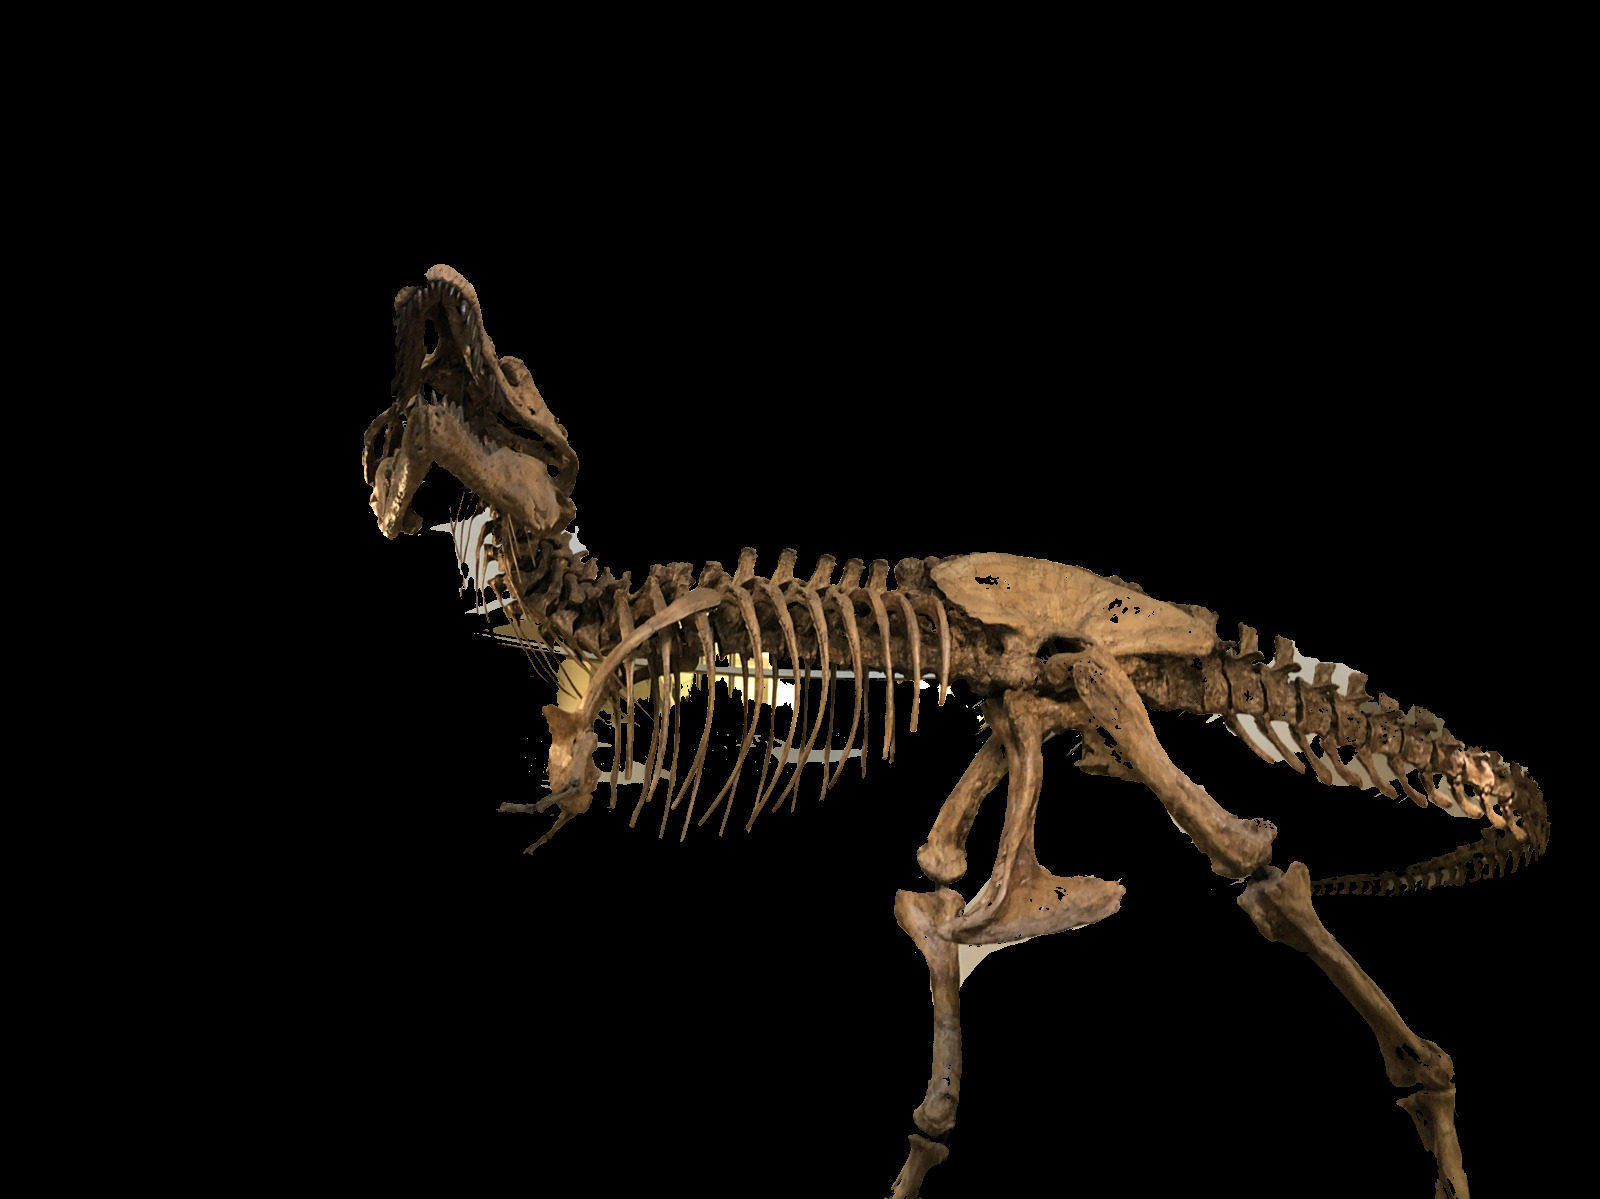
\includegraphics[width=0.2\linewidth]{figures/diffusion_appendix/trex_pred.jpg} \\
    \caption{\textbf{Illustration of the graph diffusion process.} 2D projections of i) first three PCA components of DINOv2 3D features, ii) unary regularization term (red), iii) weight vector $g_t$ at timesteps $t\in \{0,3,5,10,100\}$, iv) RGB segmentation obtained using a mask based on the 2D projection of $g_{100}$.}
    \label{fig:appendix-diffusion}
\end{figure*}

\myparagraph{Object removal} Fig.~\ref{fig:appendix-object-removal} shows comparative visualizations of object removal with N3F~\citep{tschernezki2022n3f} and LUDVIG. For rendering the edited RGB image, N3F sets to zero the occupancy for all 3D points belonging to the object. For LUDVIG, we remove all Gaussians pertaining to the 3D semantic mask resulting from graph diffusion. We observe that the regions behind to segmented object are much smoother for LUDVIG than for N3F. Regions unseen from any viewpoint are black for LUDVIG (no gaussians) and result in a background partially hallucinated by NeRF for N3F.  

\begin{figure*}[t!]
    \centering
    \begin{subfigure}{.32\linewidth}
        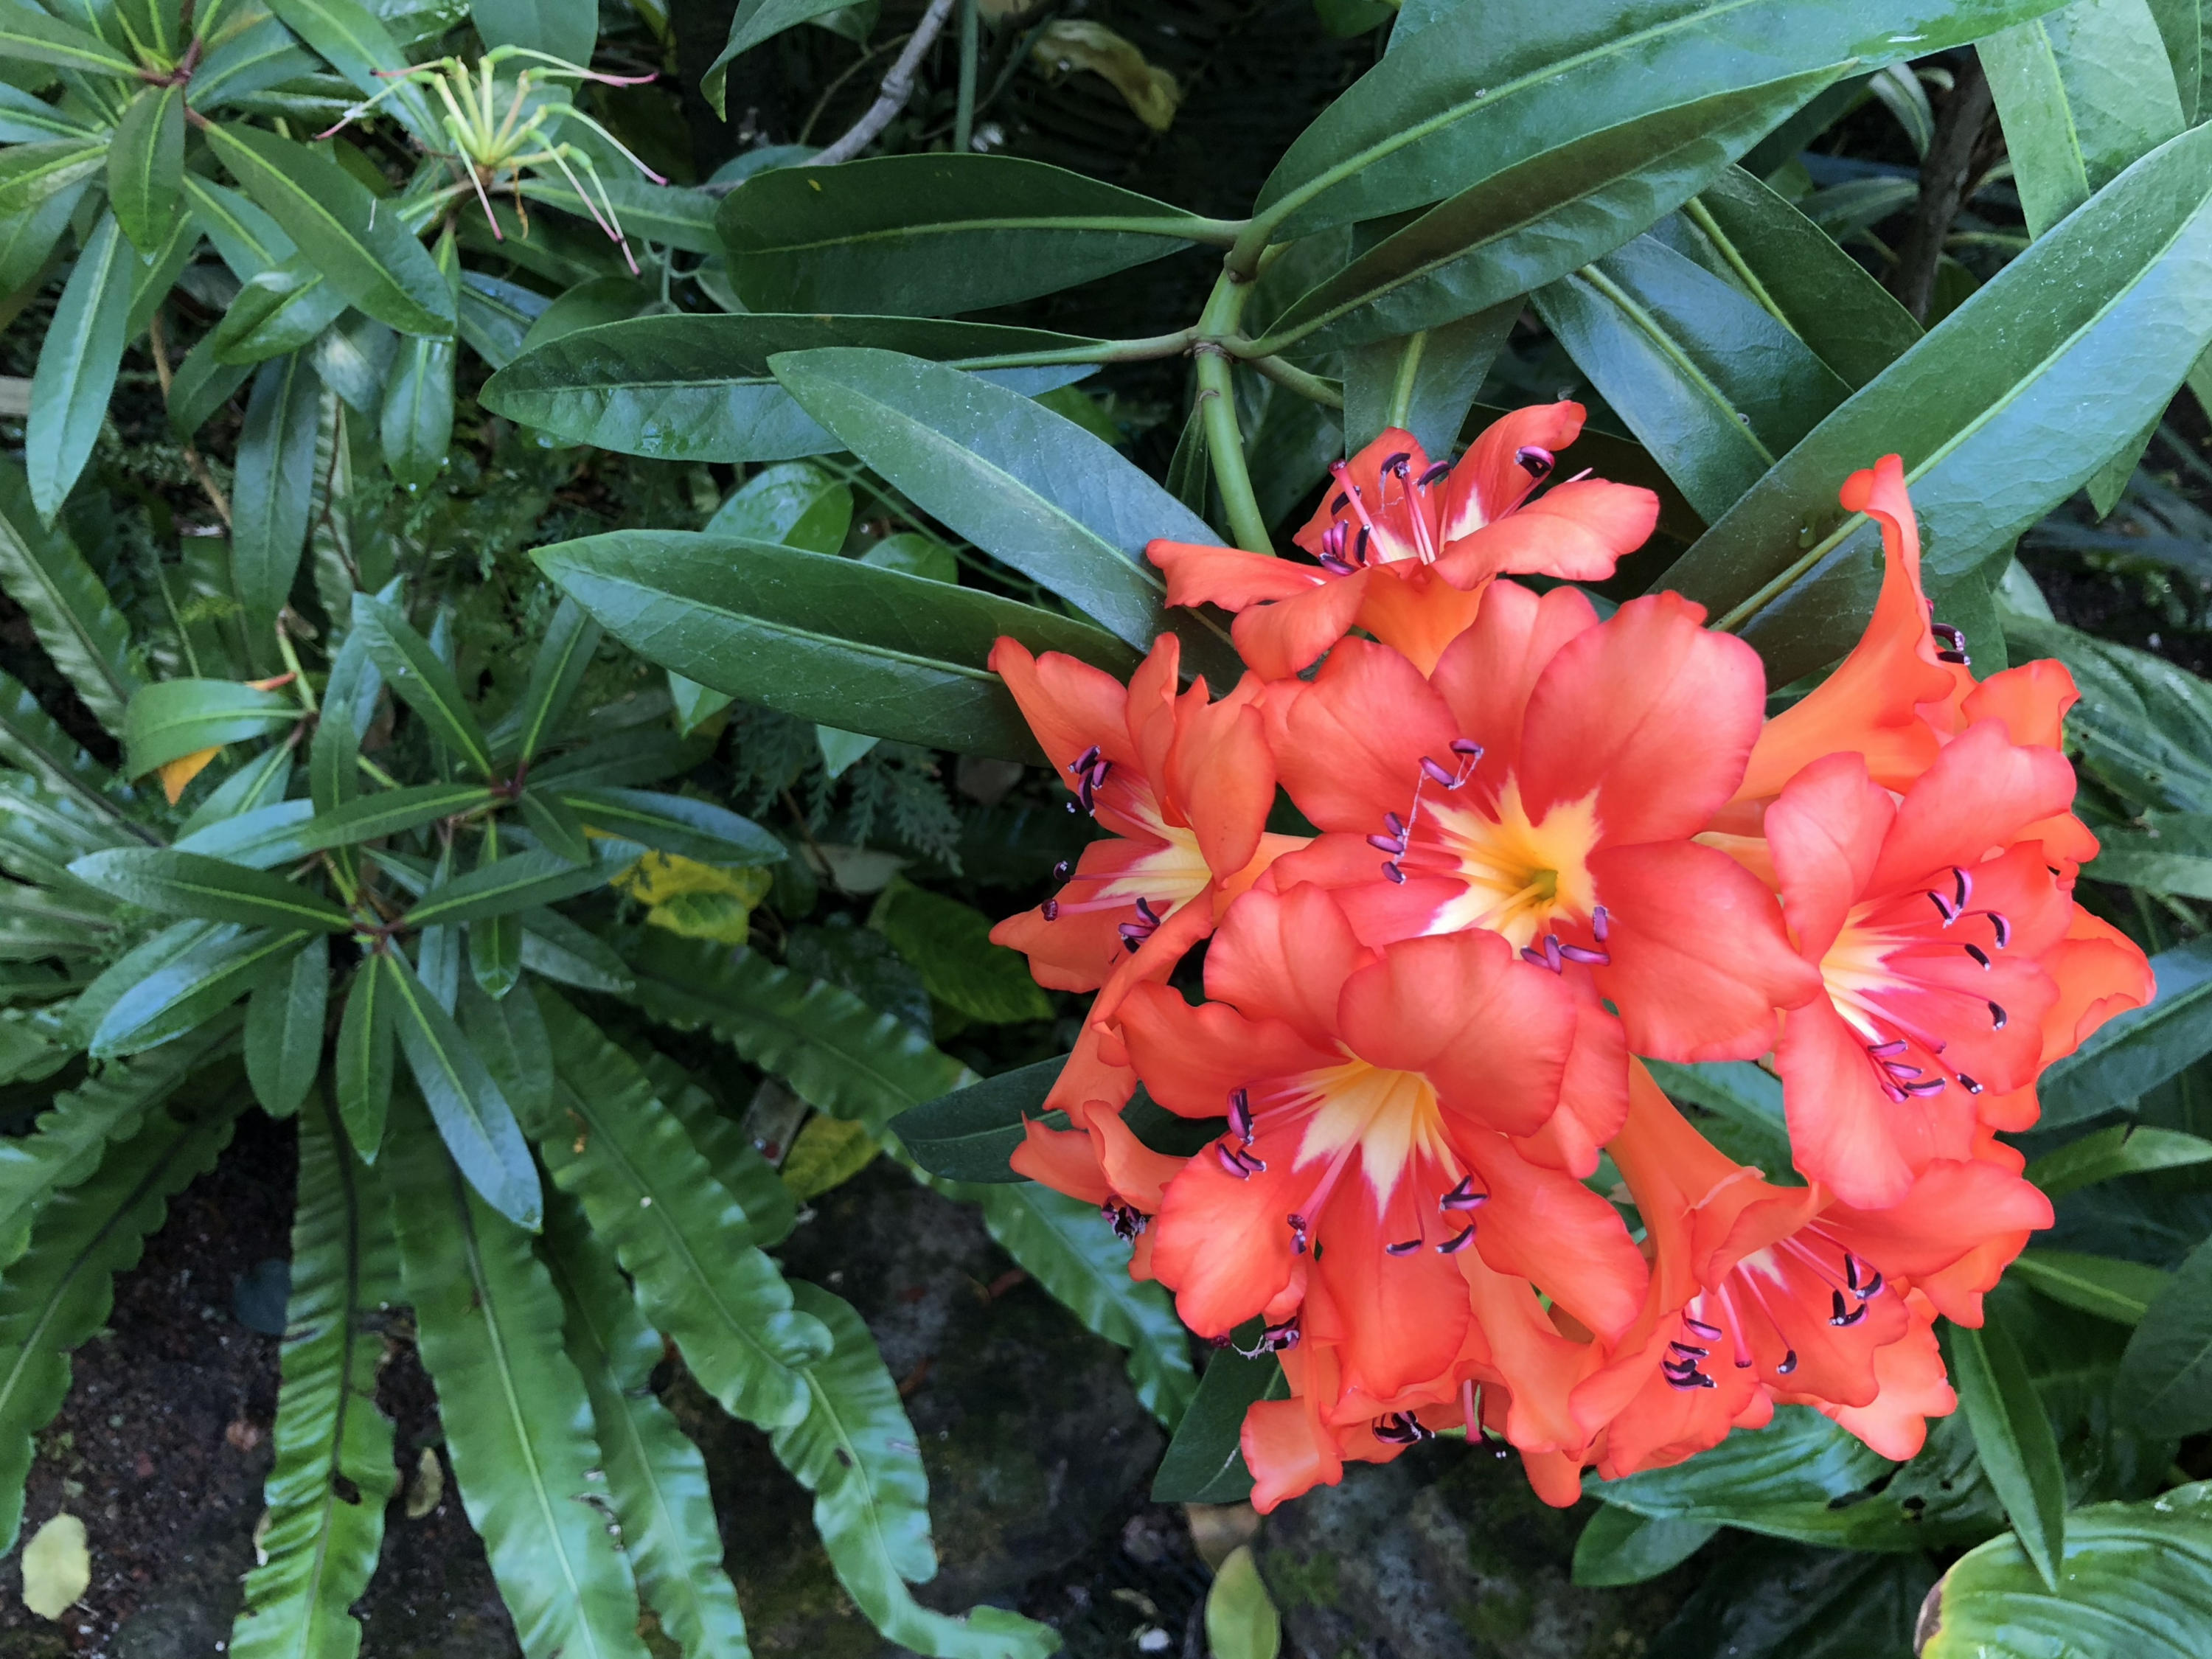
\includegraphics[width=\linewidth, trim=0 360 0 360, clip]{figures/editing/flower.jpg} \\
        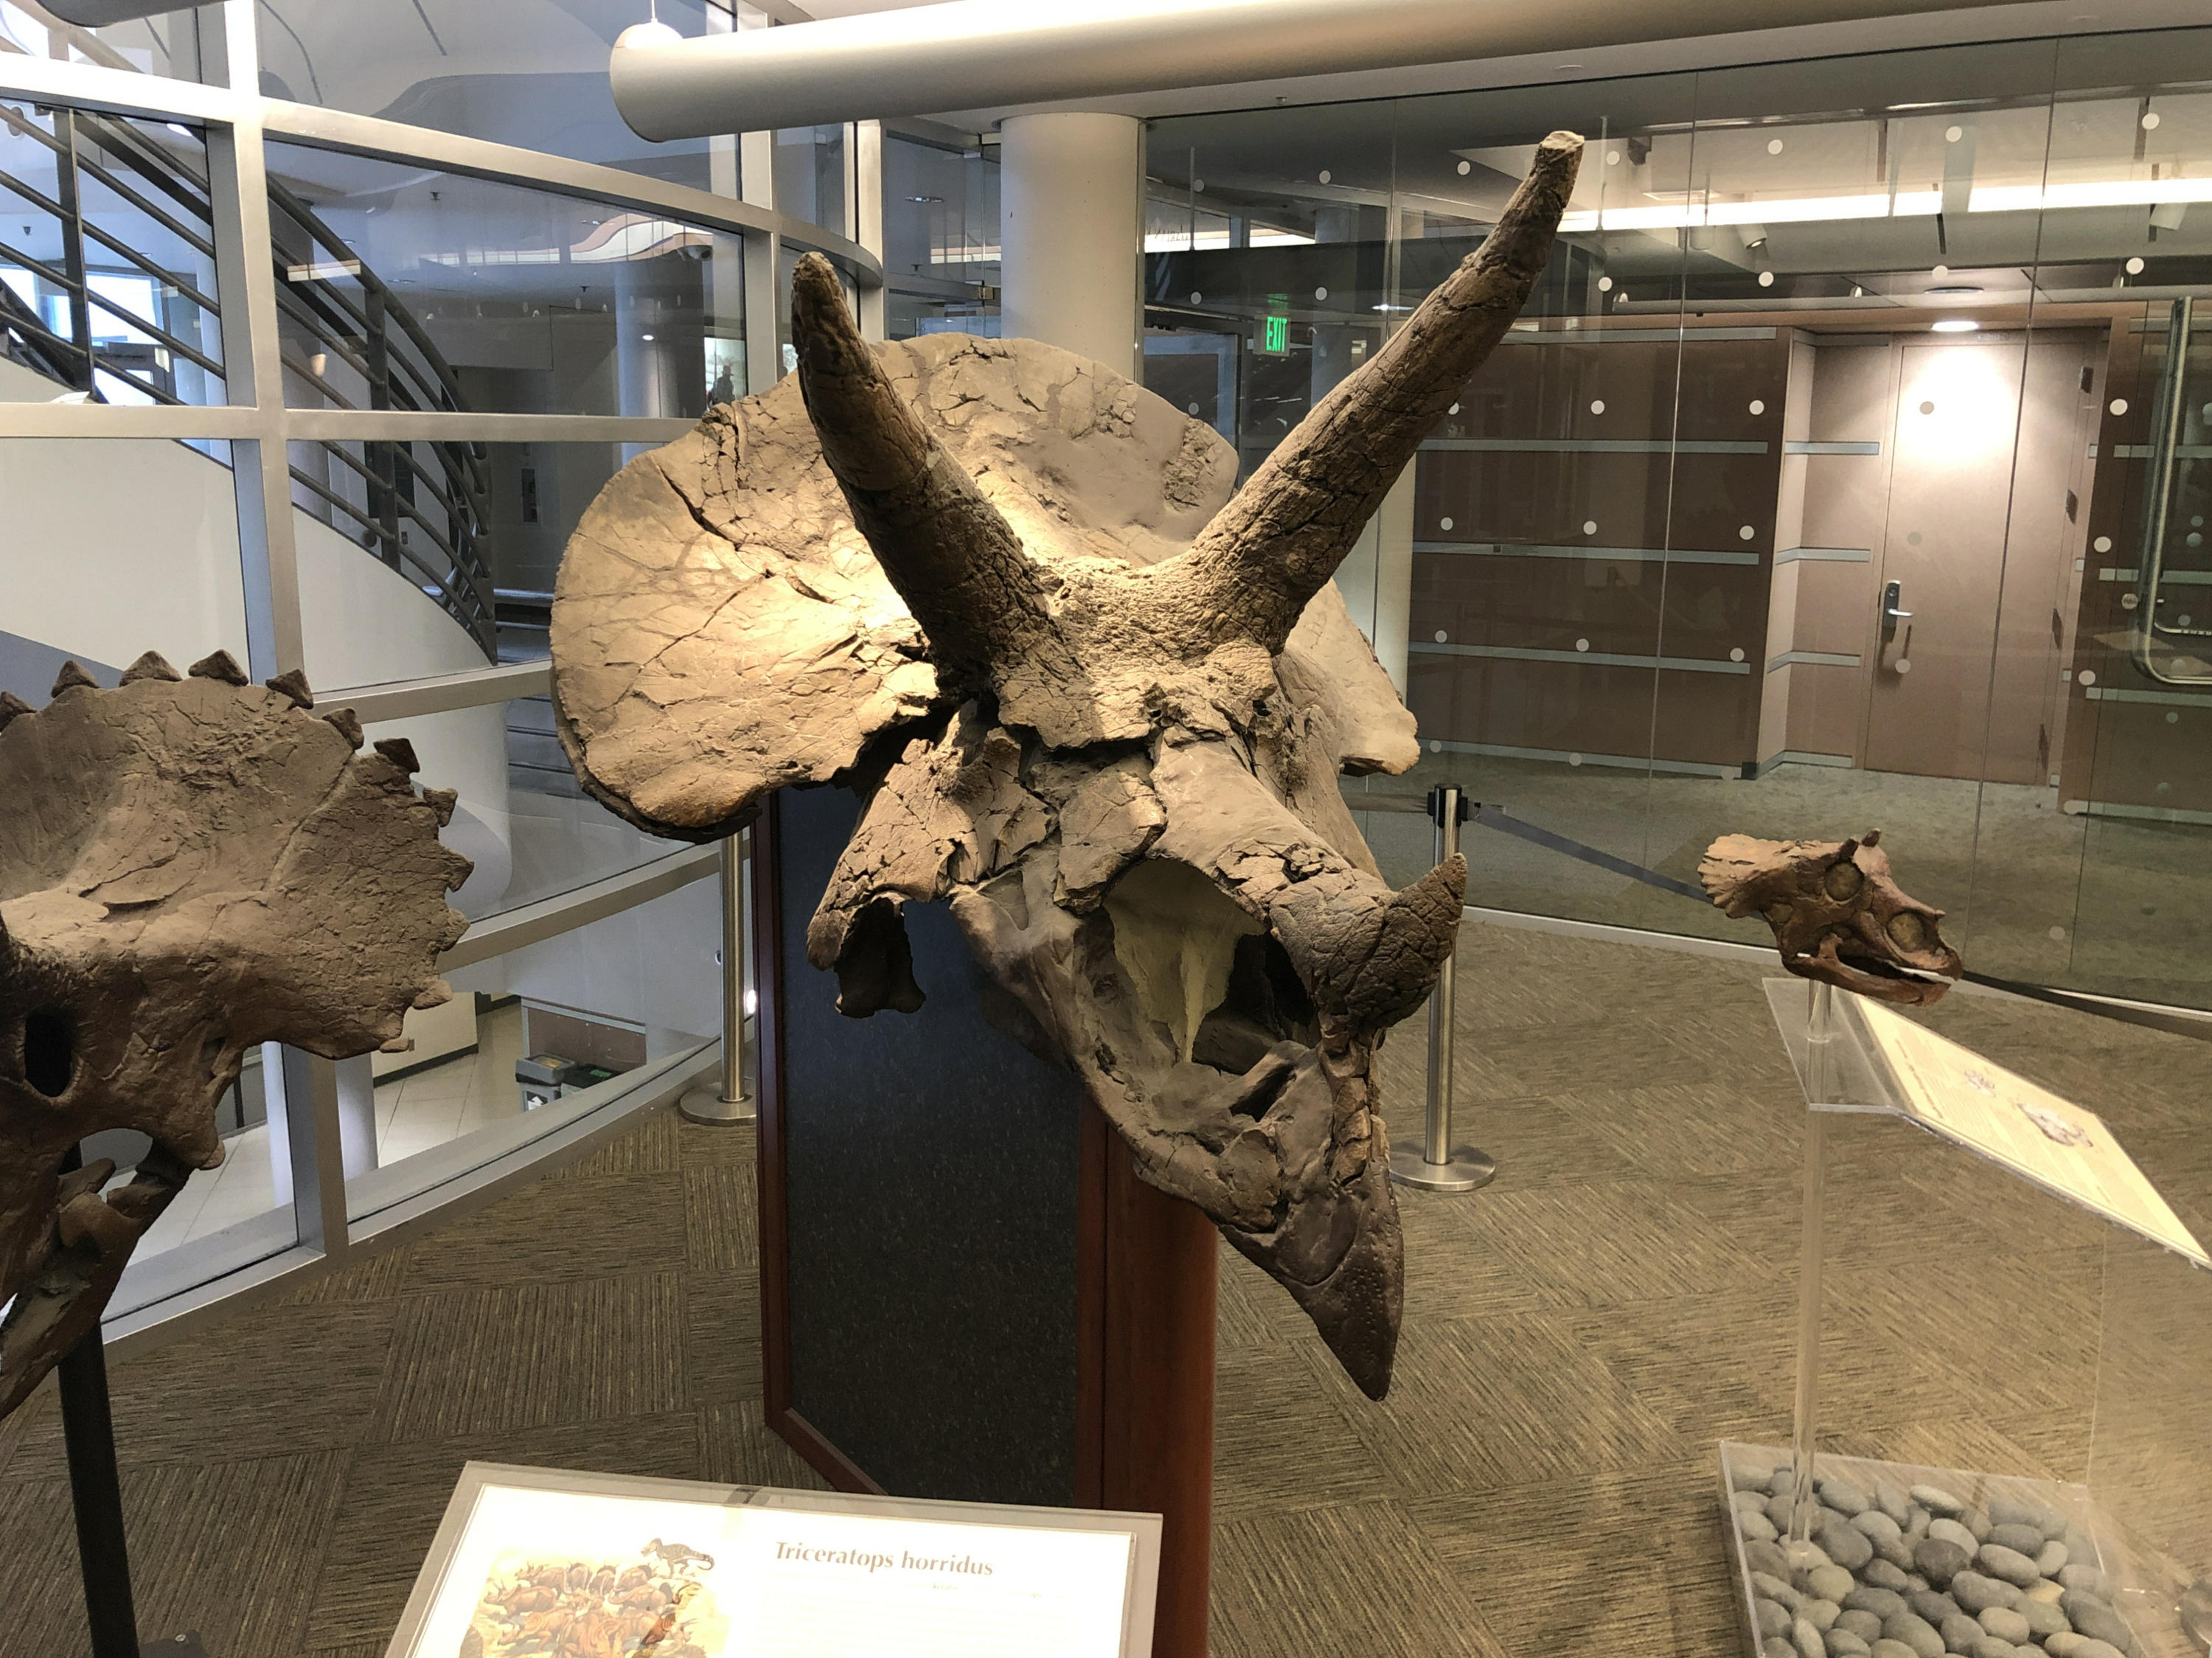
\includegraphics[width=\linewidth, trim= 0 360 0 360, clip]{figures/editing/horns.jpg} \\
        \caption{RGB image}
    \end{subfigure}
    \begin{subfigure}{.32\linewidth}
        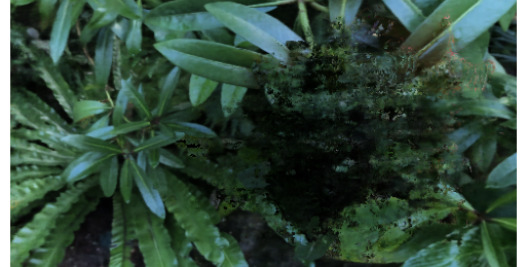
\includegraphics[width=\linewidth]{figures/editing/n3f_flower.jpg} \\
        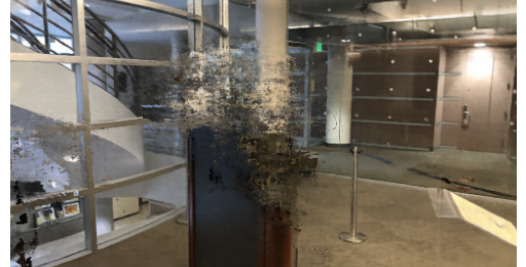
\includegraphics[width=\linewidth]{figures/editing/n3f_horns.jpg} \\
        \caption{N3F~\citep{tschernezki2022n3f}}
    \end{subfigure}
    \begin{subfigure}{.32\linewidth}
        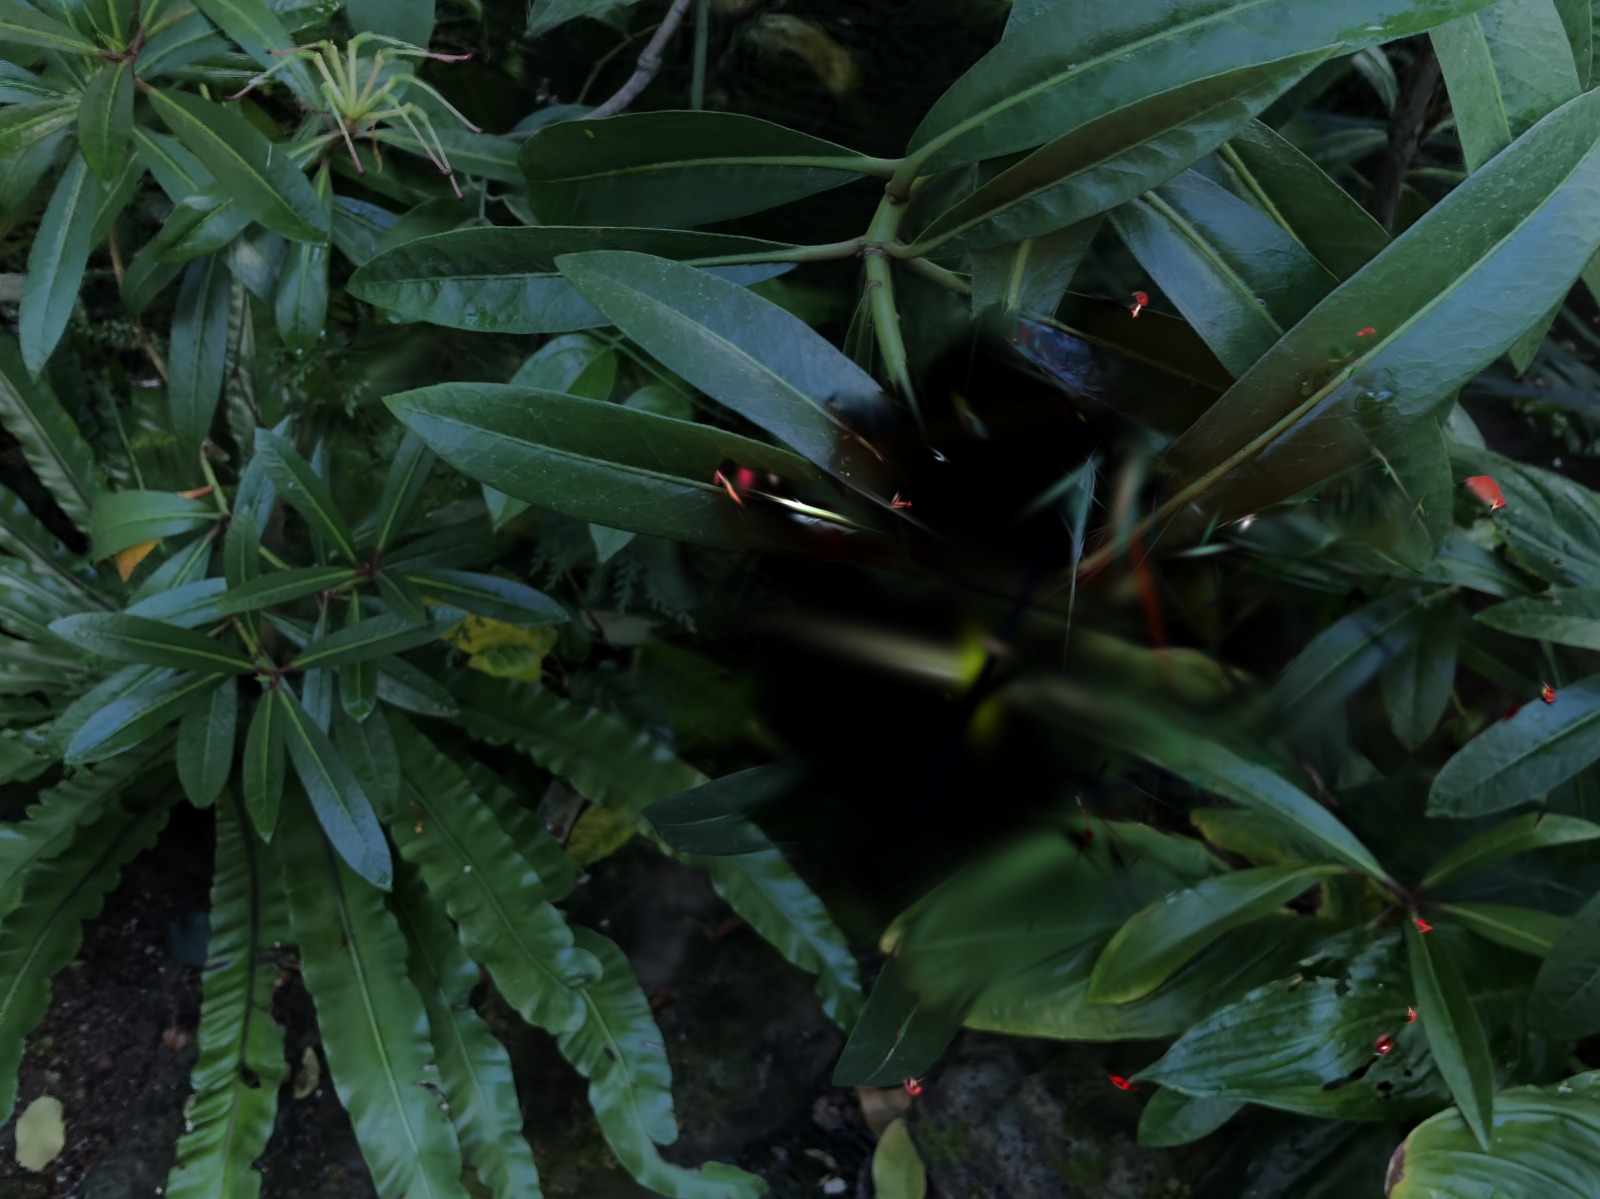
\includegraphics[width=\linewidth, trim=0 195 0 195, clip]{figures/editing/ludvig_flower_bright.jpg} \\
        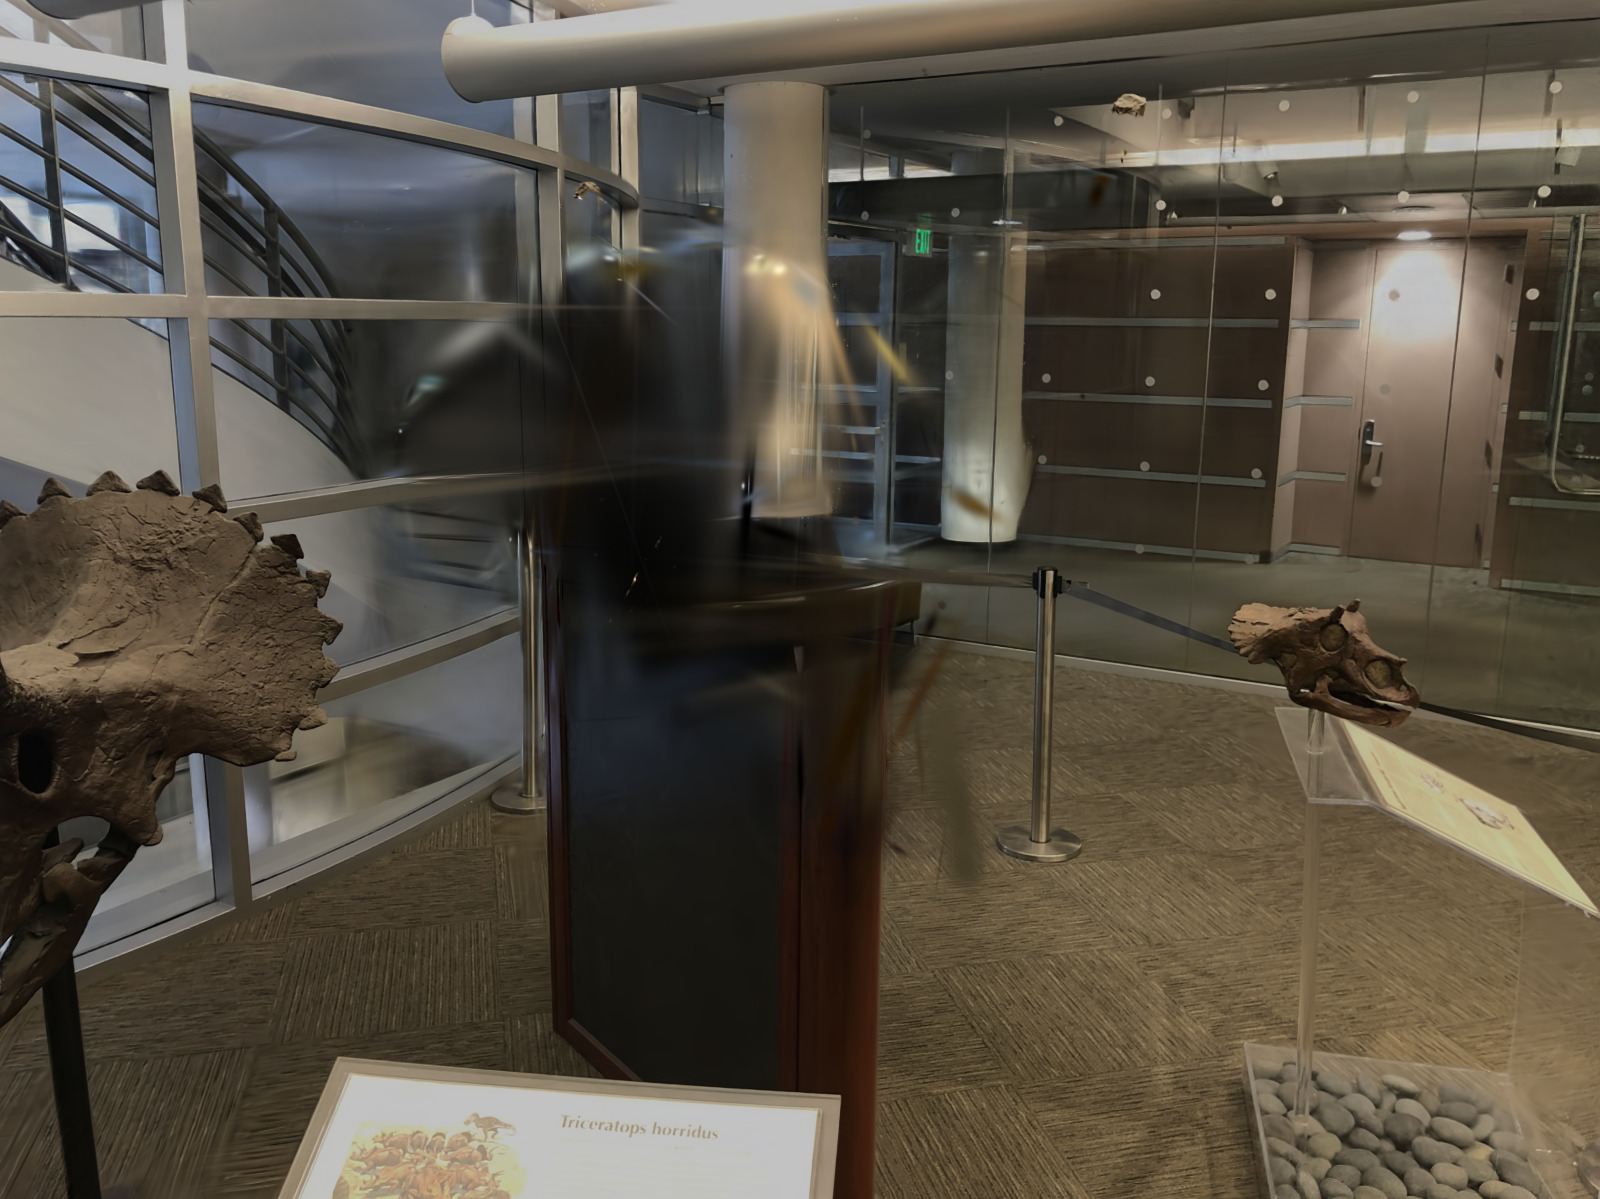
\includegraphics[width=\linewidth, trim=0 195 0 195, clip]{figures/editing/ludvig_horns.jpg} \\
        \caption{LUDVIG (ours)}
    \end{subfigure}
    \caption{\textbf{Object removal.} 3D segmentation, removal and rendering for LUDVIG and N3F~\citep{tschernezki2022n3f}. For N3F, figures are taken from~\citep{tschernezki2022n3f}.}
    \label{fig:appendix-object-removal}
\end{figure*}

\subsection{Visual comparisons of uplifted features}

Fig.~\ref{fig:appendix-dff} show a comparison of LUDVIG's 3D DINOv2 features with learned 3D DINO features of N3D~\citep{tschernezki2022n3f}. Their figures are taken from their work. Compared to N3D, LUDVIG produces a more fine-grained reconstruction of the background (notably in the trex and horns scenes) and smoother features across all scenes.

\begin{figure*}[t!]
    \centering
    \begin{subfigure}{.9\linewidth}
        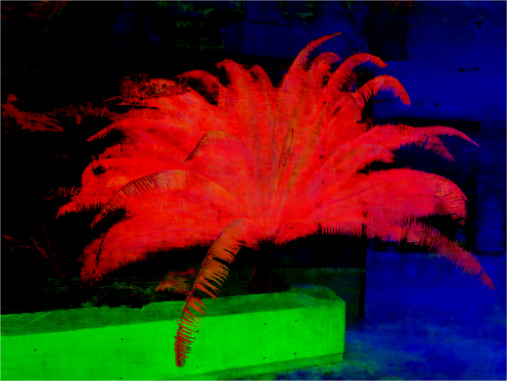
\includegraphics[width=.24\linewidth]{figures/n3f/fern.jpg}
        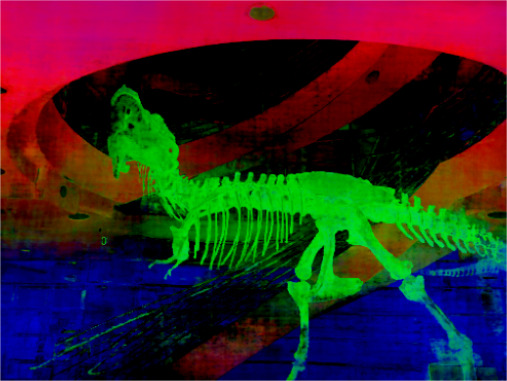
\includegraphics[width=.24\linewidth]{figures/n3f/trex.jpg}
        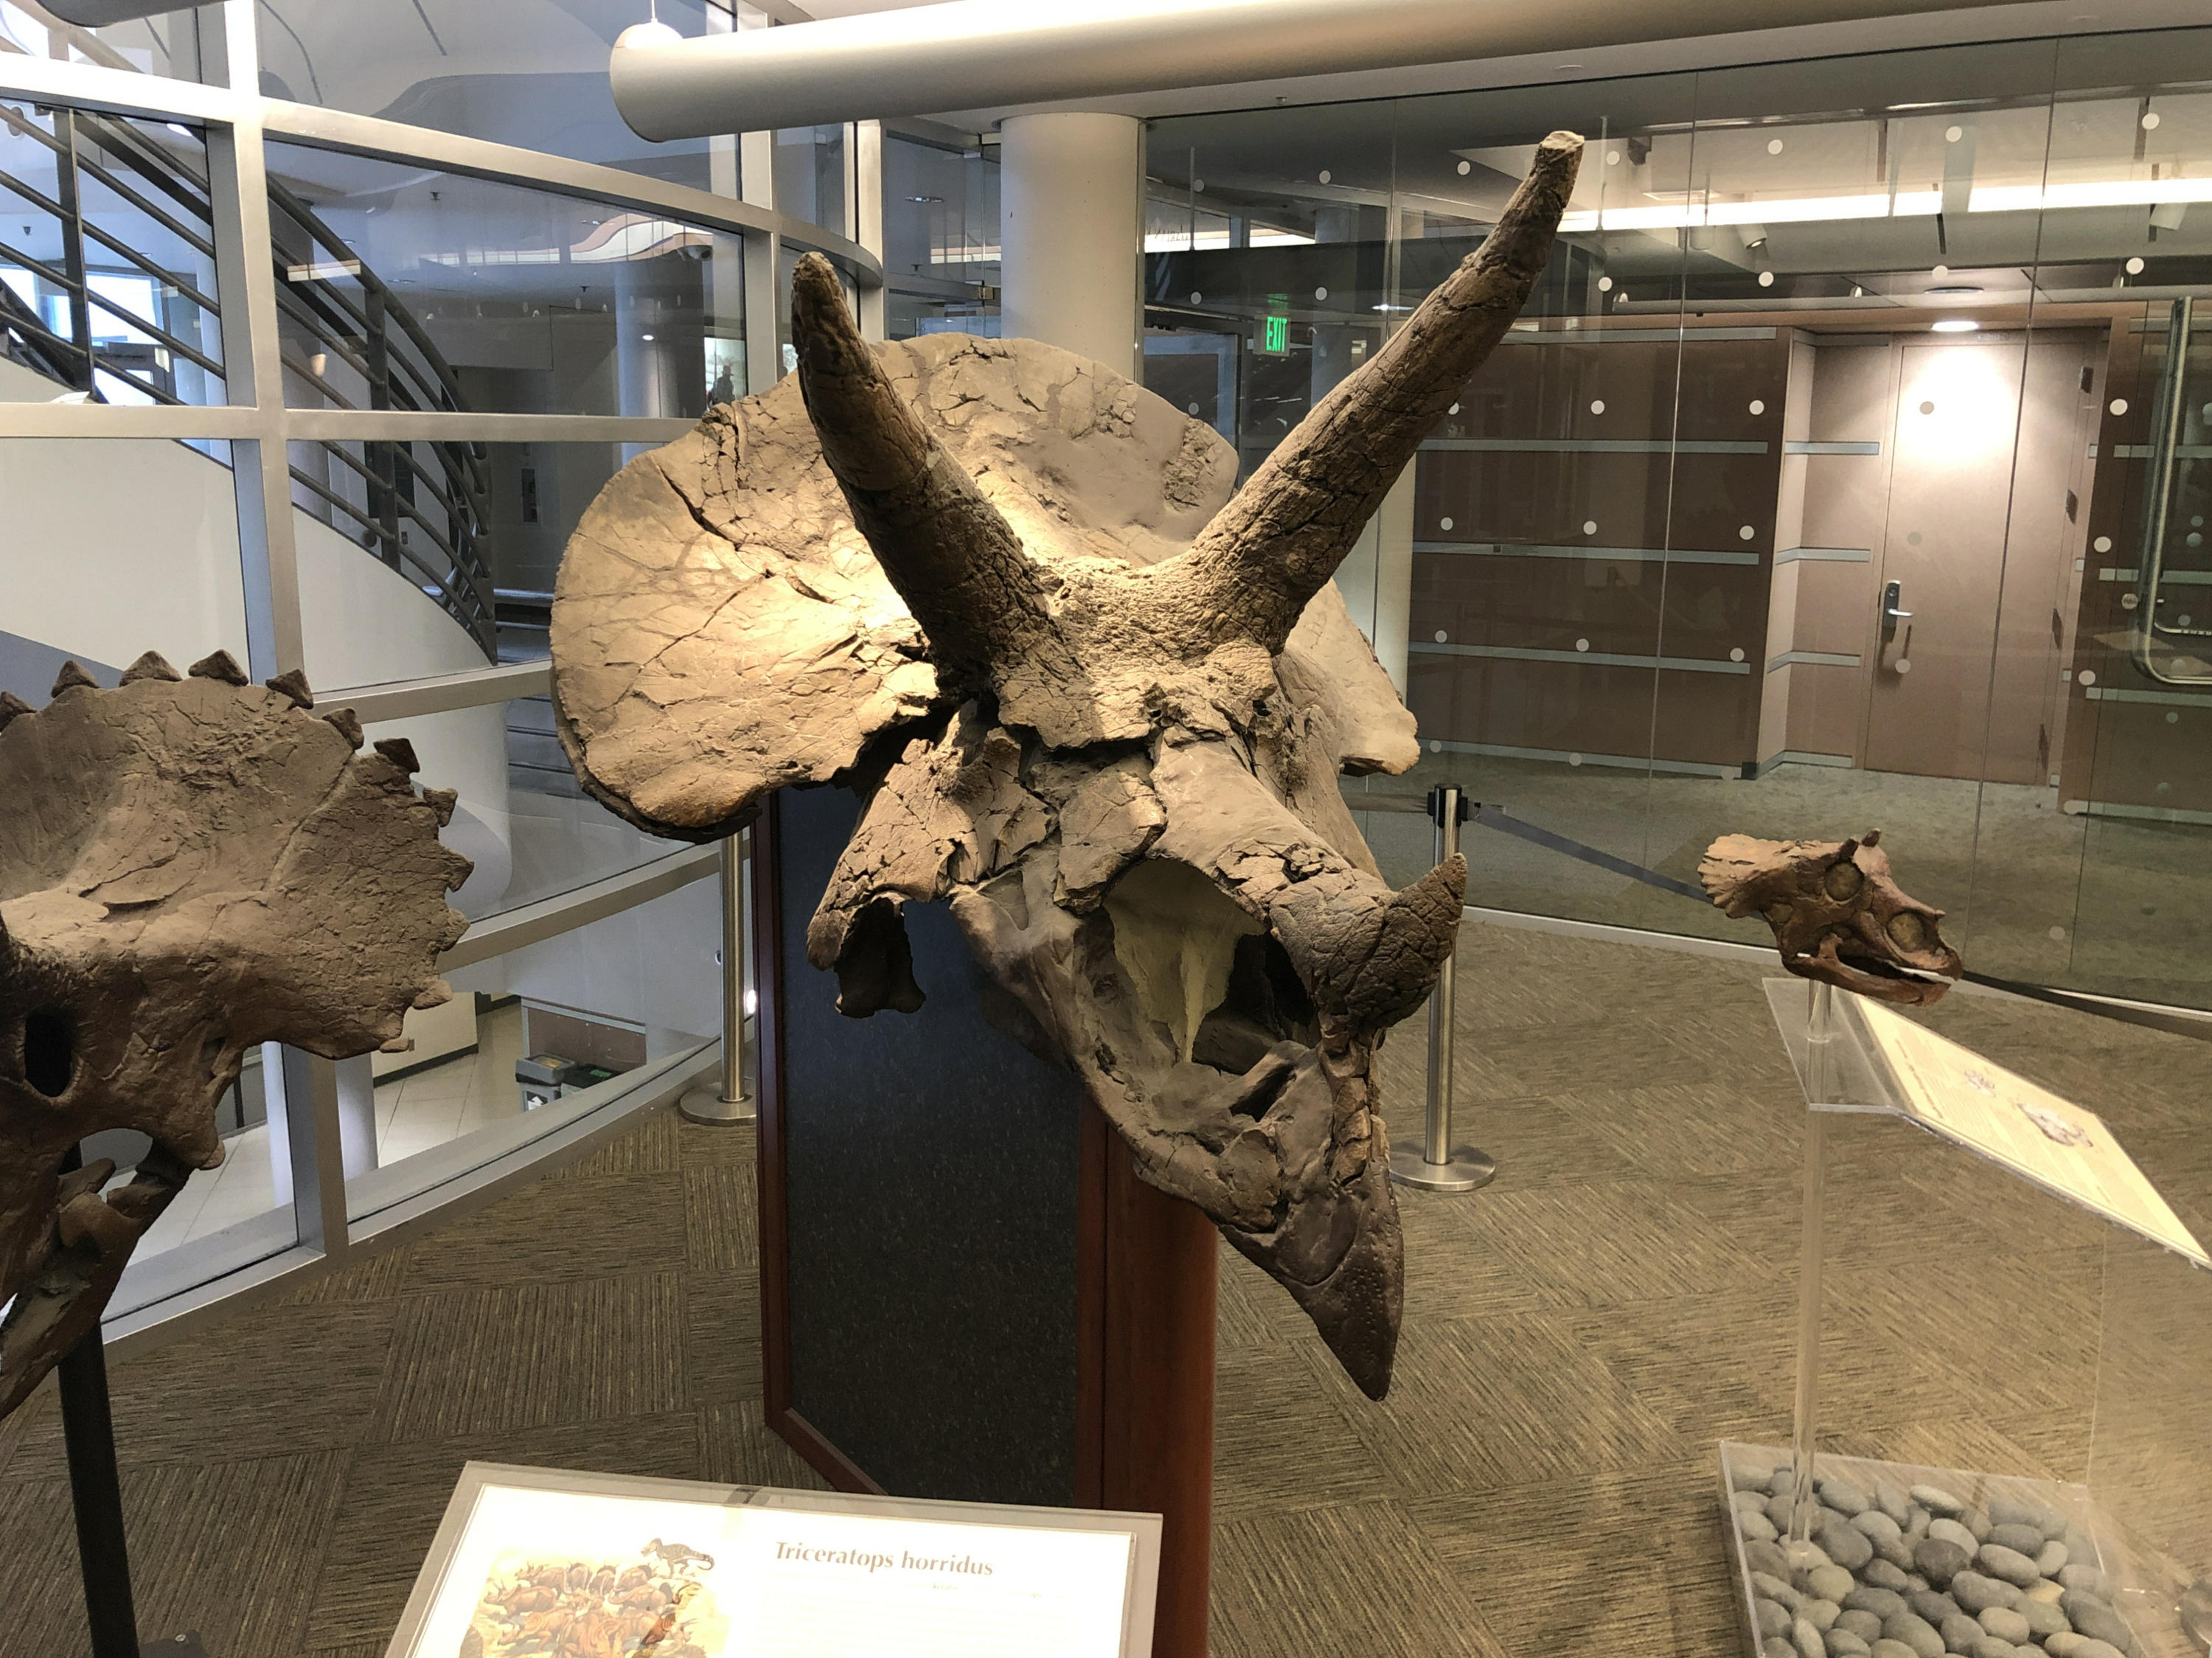
\includegraphics[width=.24\linewidth]{figures/editing/horns.jpg} 
        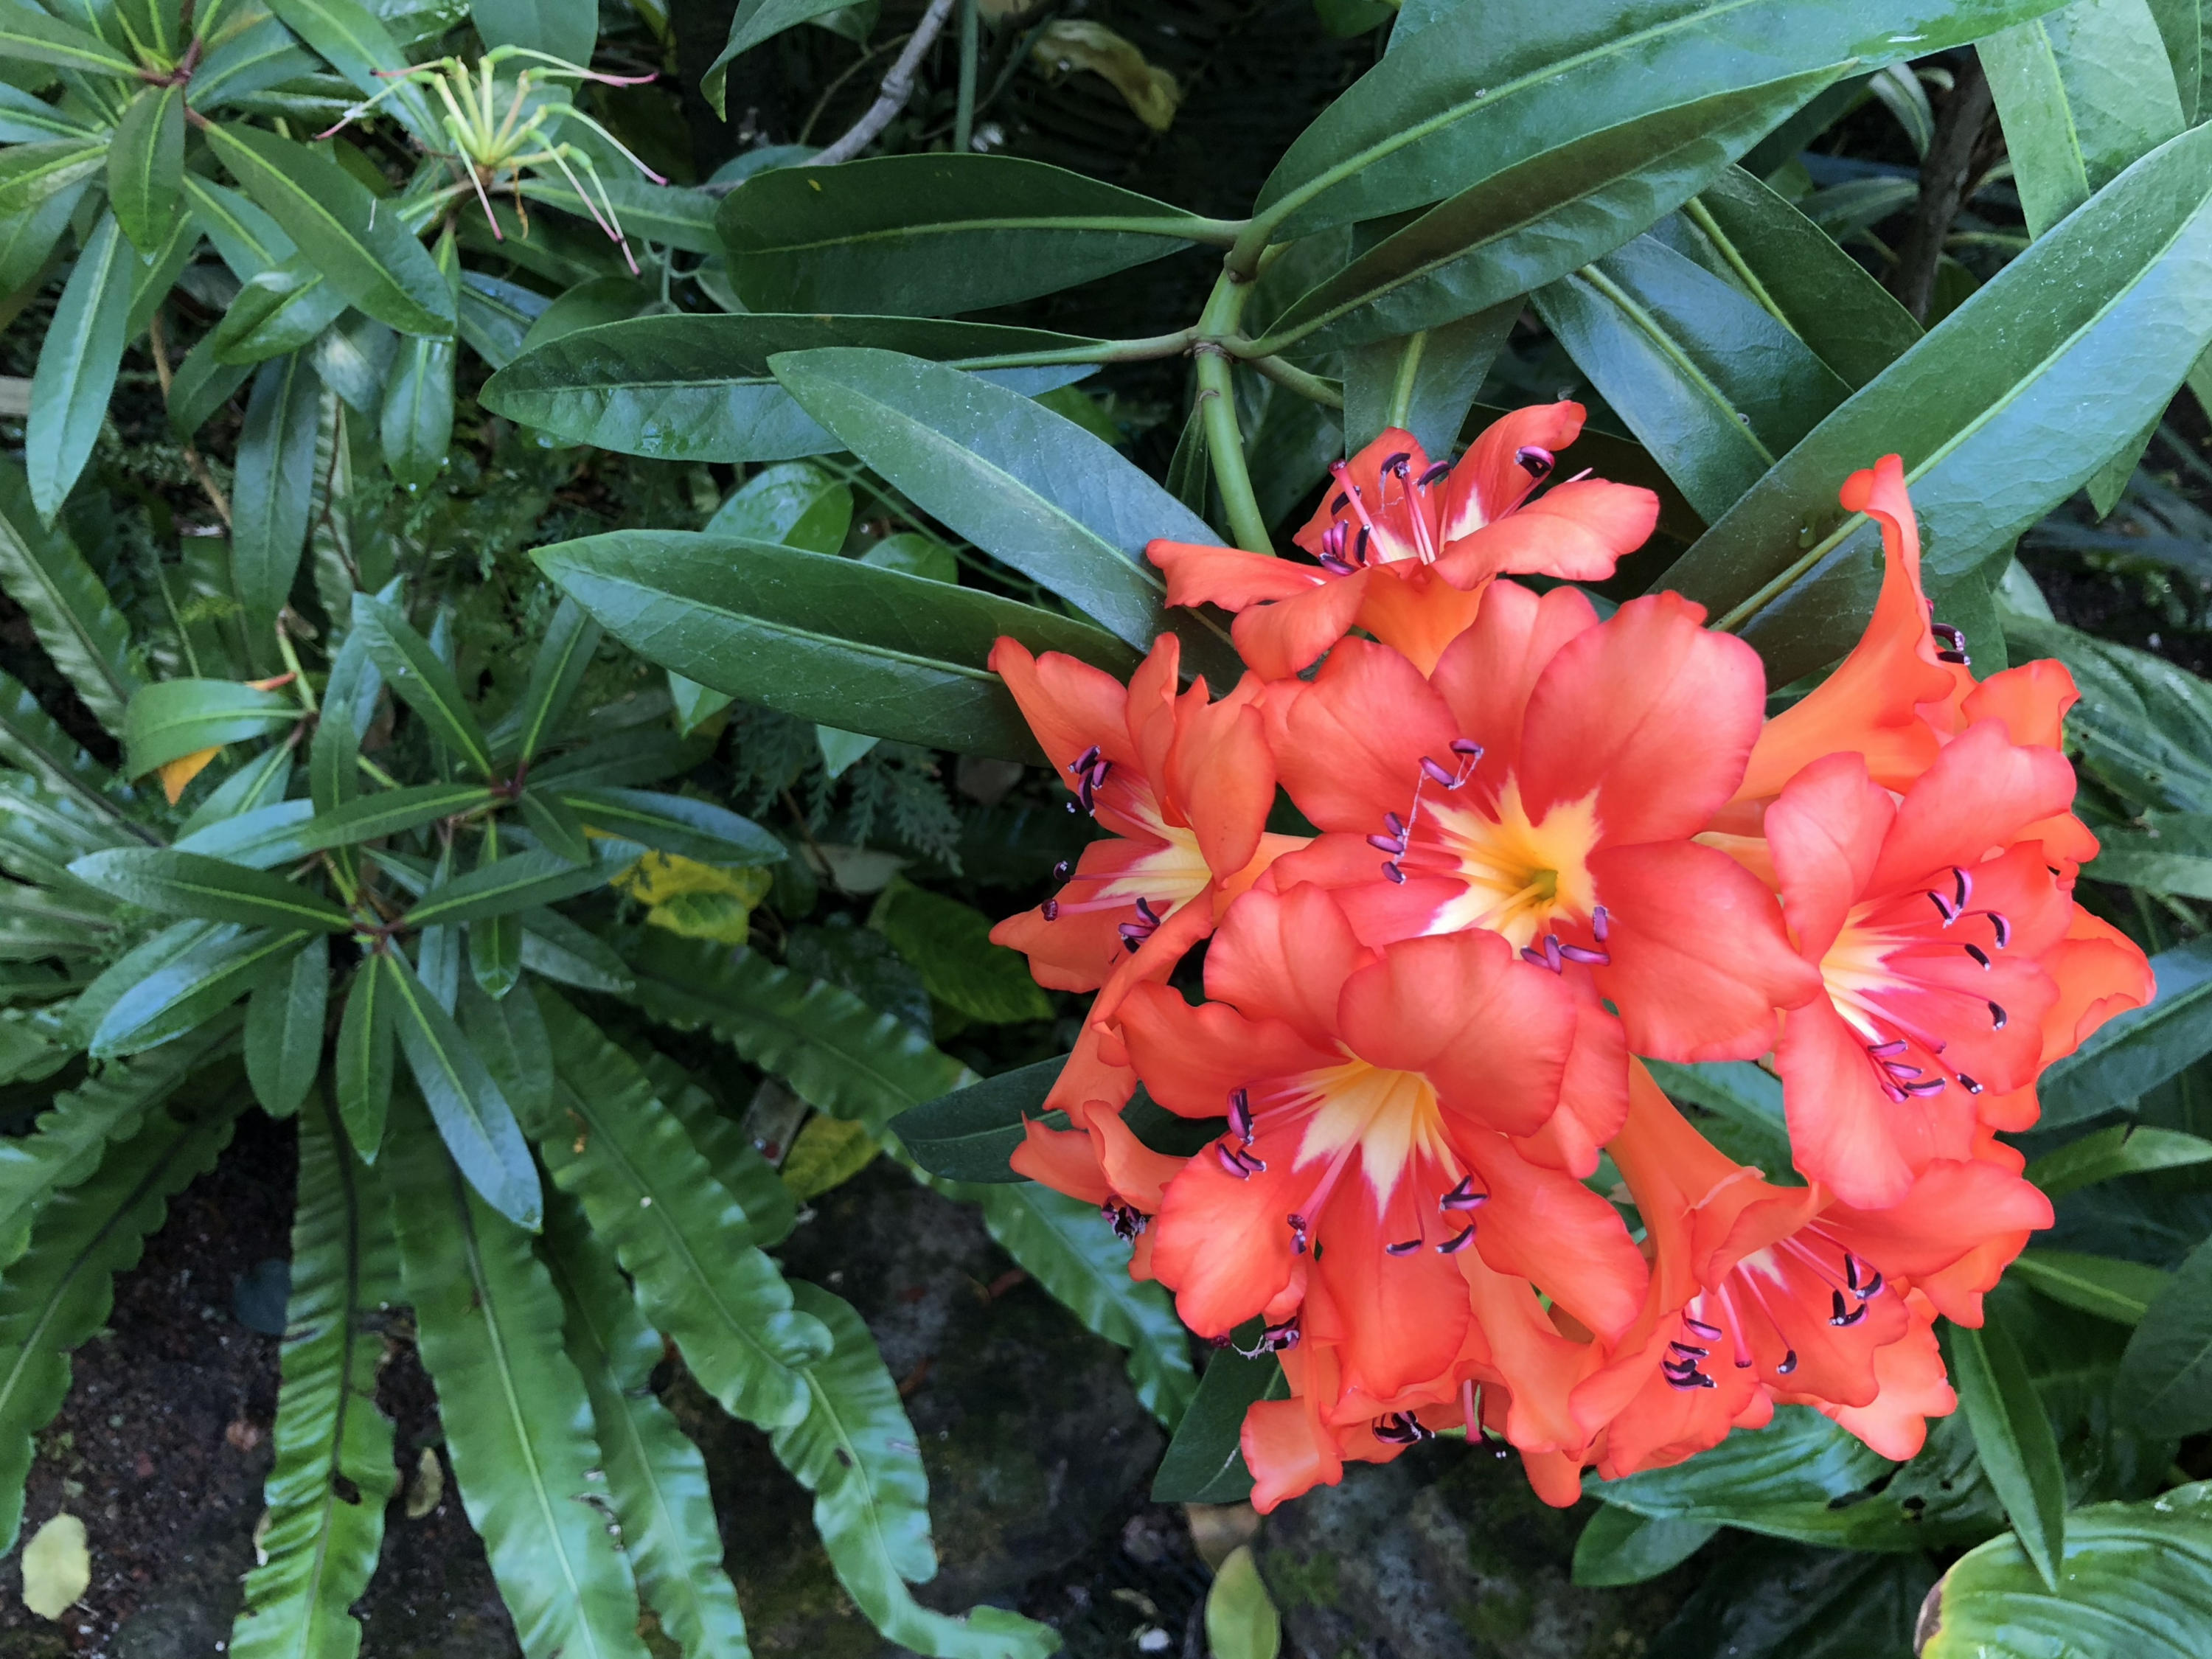
\includegraphics[width=.24\linewidth]{figures/editing/flower.jpg} 
    \end{subfigure}
    \begin{subfigure}{.9\linewidth}
        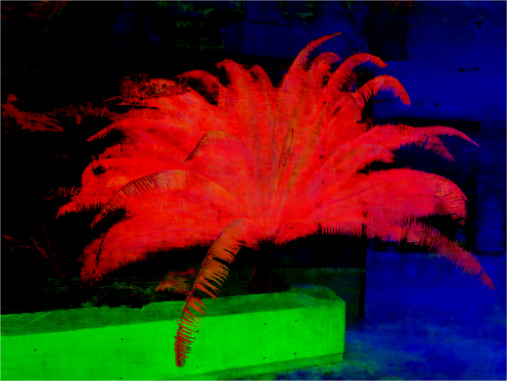
\includegraphics[width=.24\linewidth]{figures/n3f/fern.jpg}
        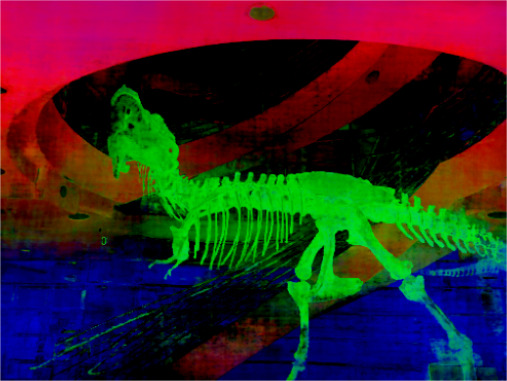
\includegraphics[width=.24\linewidth]{figures/n3f/trex.jpg}
        
\includegraphics[width=.24\linewidth]{figures/n3f/horns.jpg} 
        
\includegraphics[width=.24\linewidth]{figures/n3f/flower.jpg} 
    \end{subfigure}
    \begin{subfigure}{.9\linewidth}
        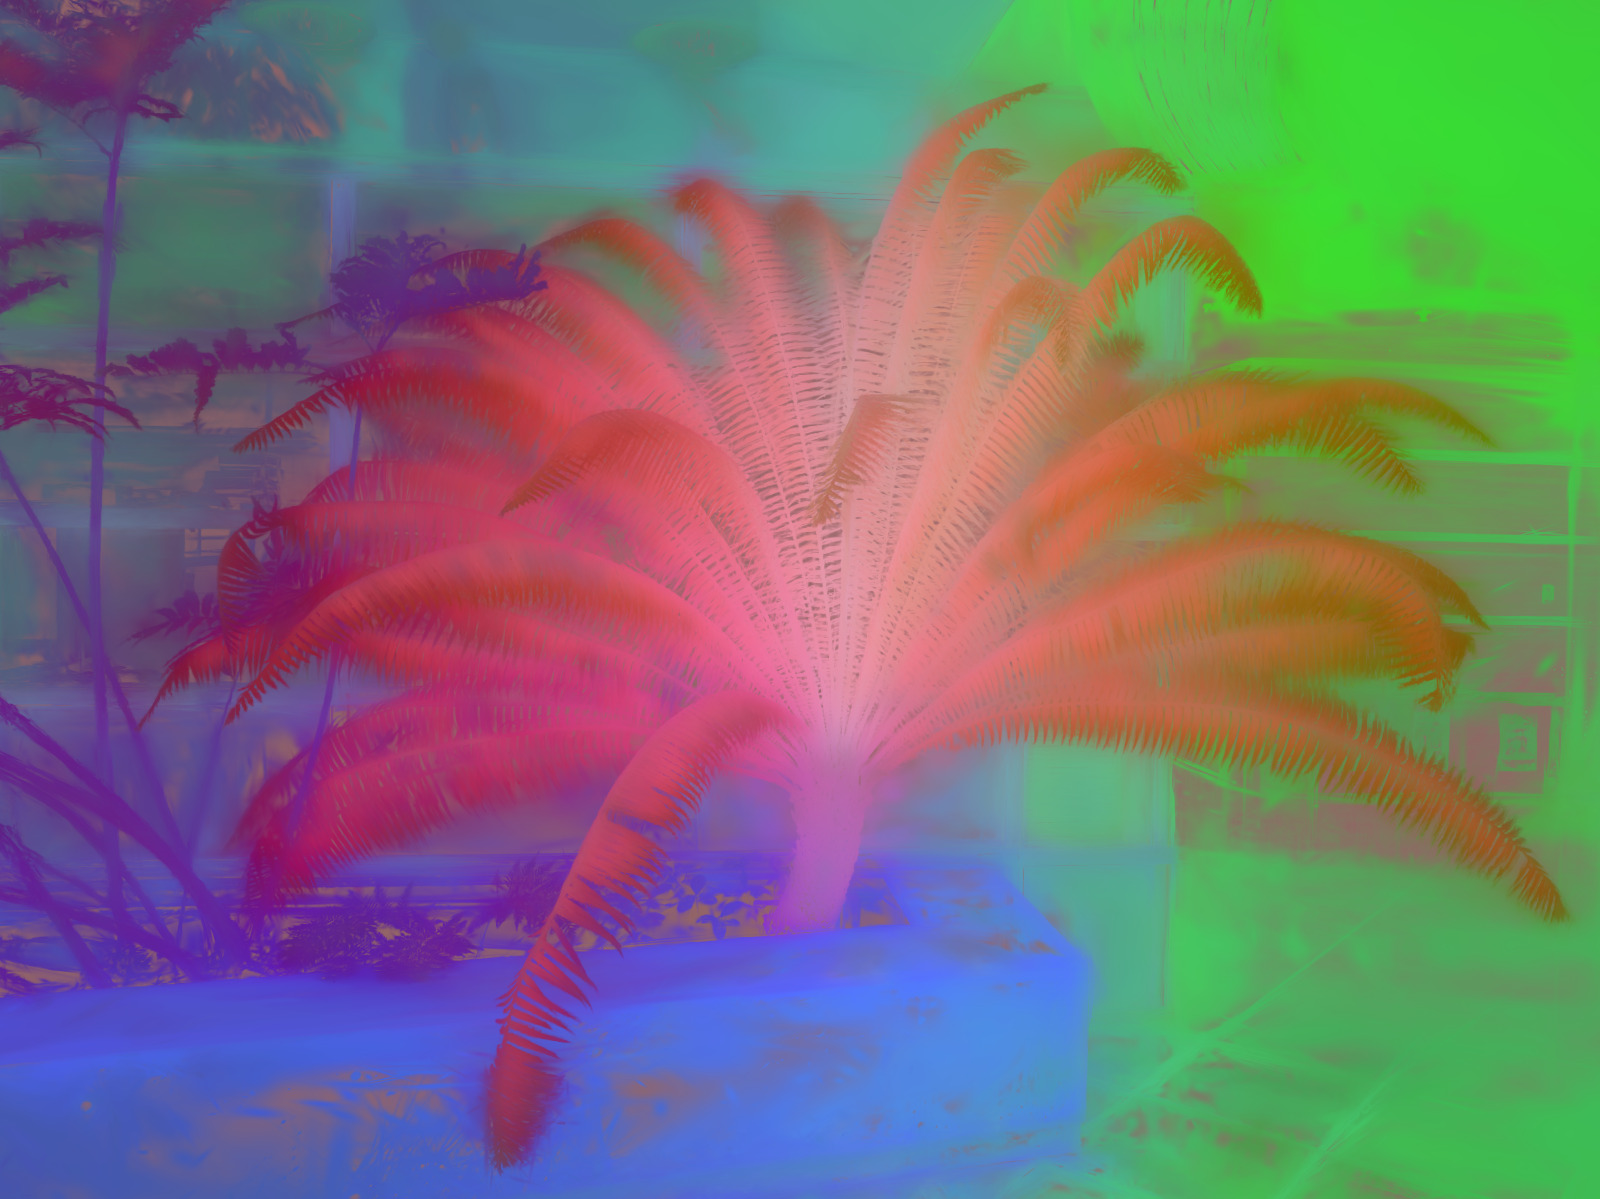
\includegraphics[width=.24\linewidth]{figures/diffusion_appendix/fern_pca.jpg} 
        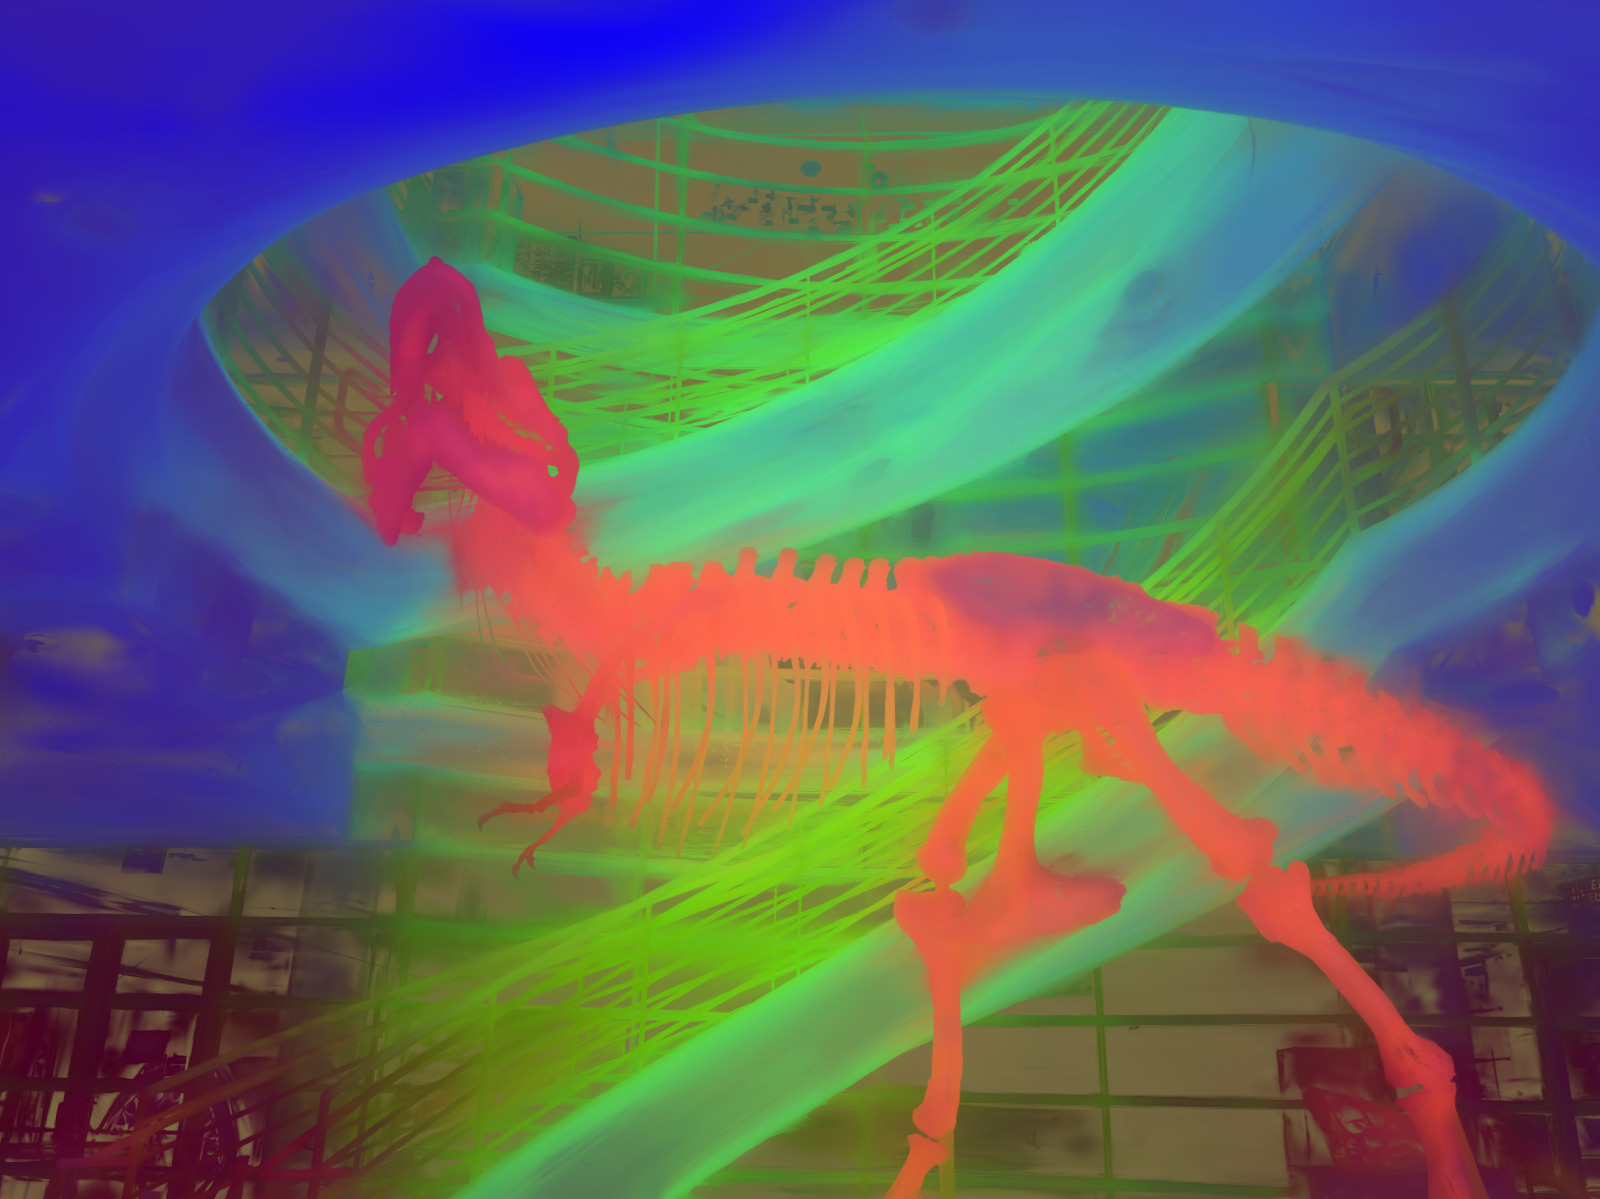
\includegraphics[width=.24\linewidth]{figures/pcas/trex_pca.jpg} 
        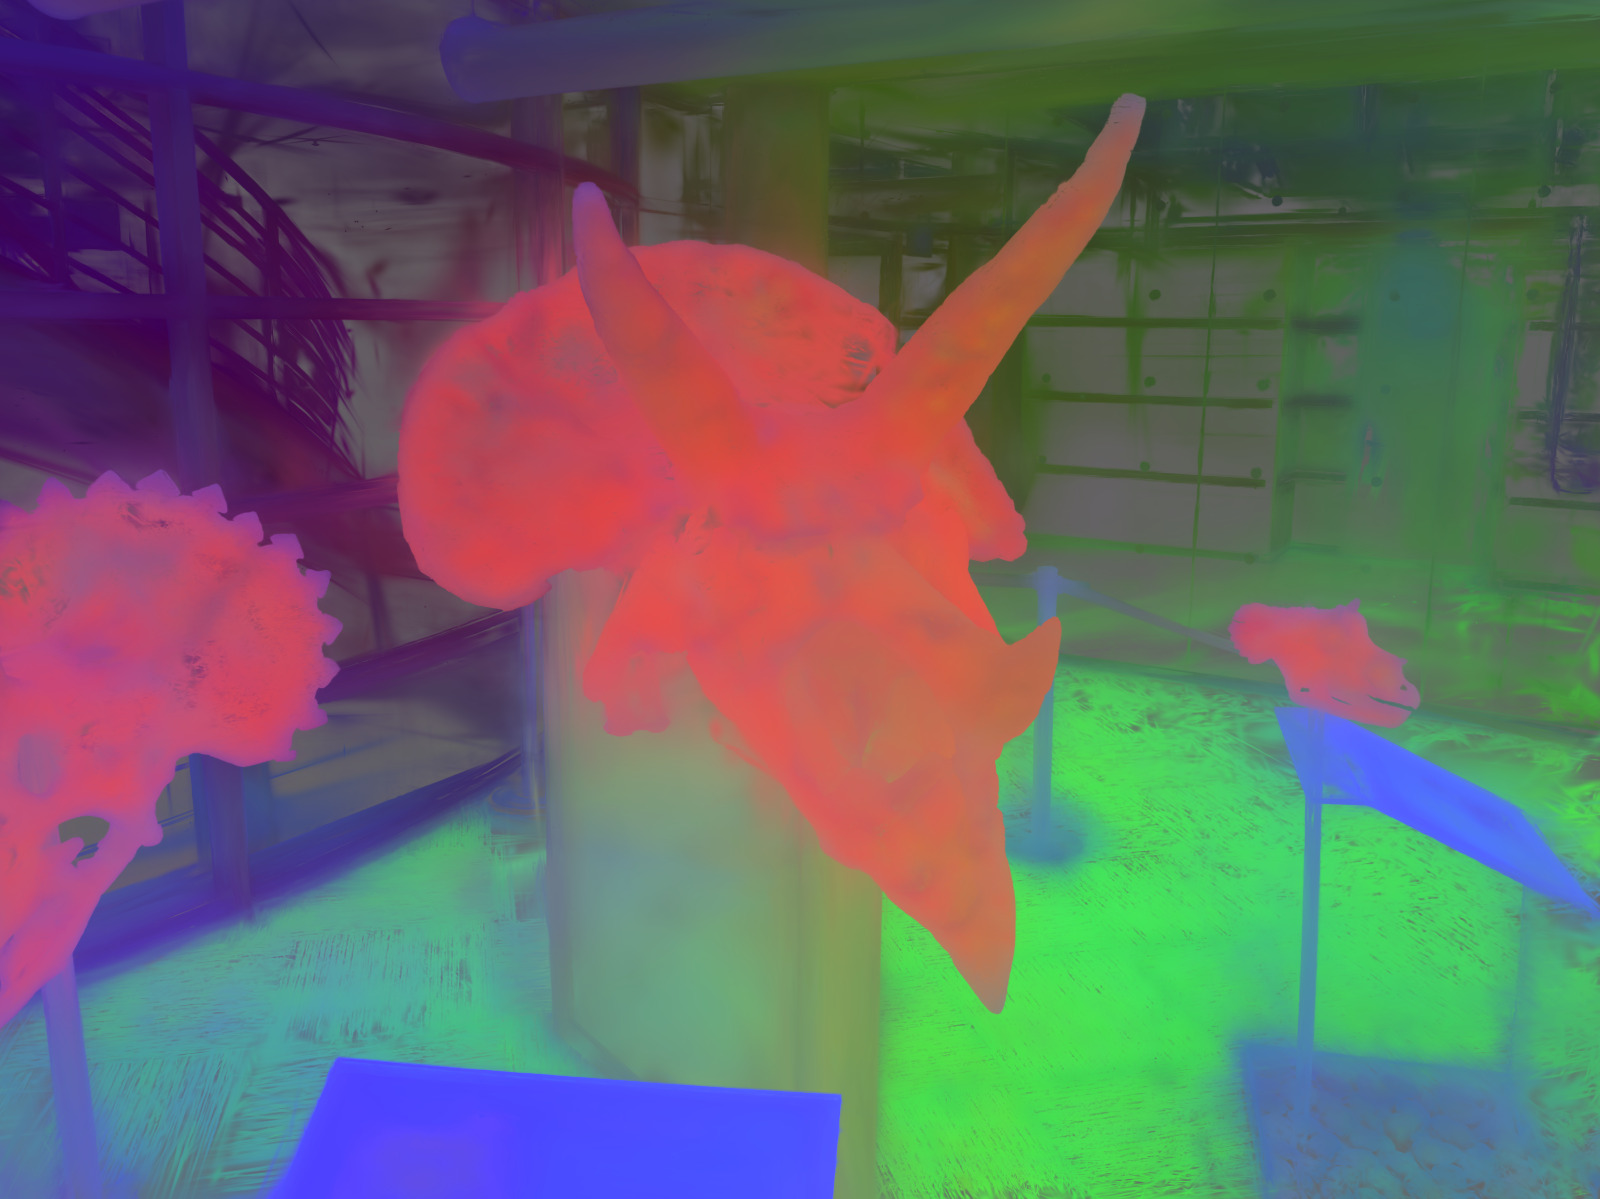
\includegraphics[width=.24\linewidth]{figures/n3f/horns_ludvig.jpg}
        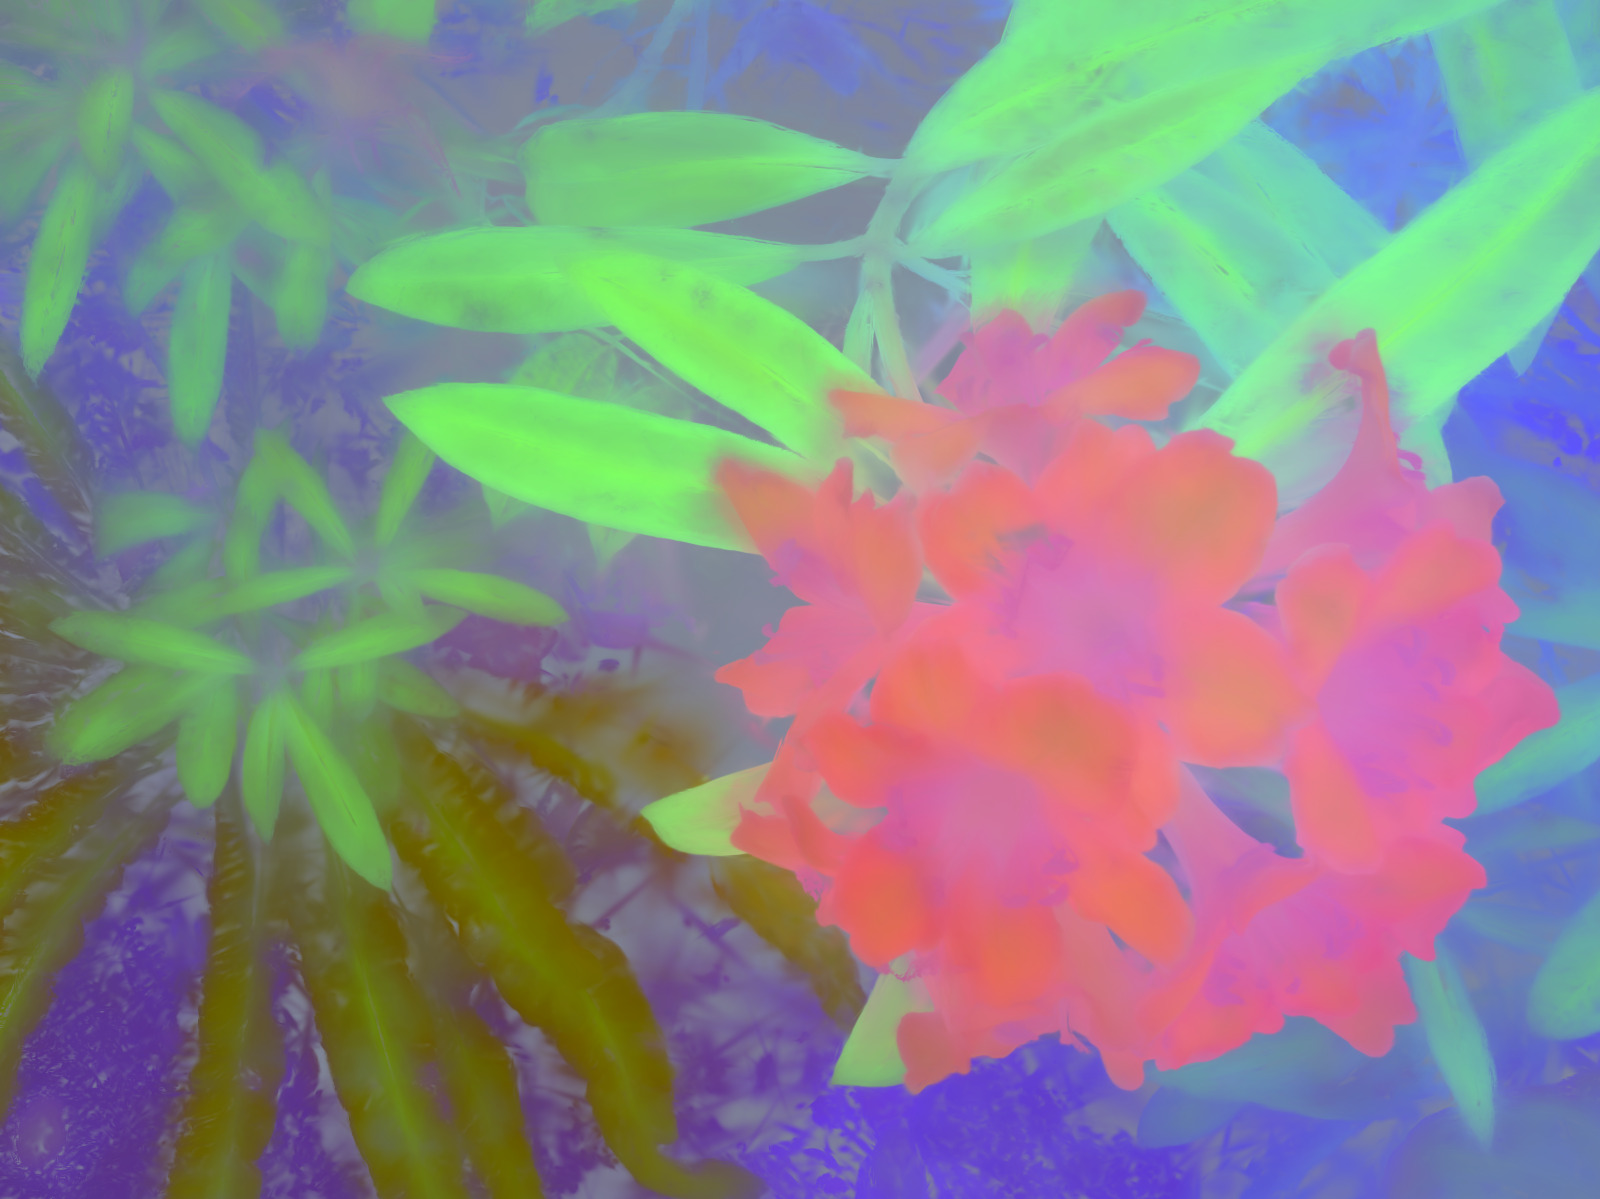
\includegraphics[width=.24\linewidth]{figures/diffusion_appendix/flower_pca.jpg}
    \end{subfigure}
    \caption{Comparison between LUDVIG's uplifted DINOv2 features (bottom) and N3F's~\citep{tschernezki2022n3f}
    learned DINO features (top). For N3F, figures are taken from ~\citep{tschernezki2022n3f}.}
    \label{fig:appendix-dff}
\end{figure*}


\subsection{3D features for ScanNet semantic segmentation}


Fig.~\ref{fig:appendix-semantic} presents visualizations of 3D semantic features obtained by uplifting 2D feature maps generated by OpenGaussian~\citep{wu2024opengaussian}. Following the approach of LangSplat~\citep{qin2023langsplat}, the 2D features are computed by assigning object-level CLIP embeddings to segmentation masks produced by SAM in \emph{everything} mode.

Surprisingly, despite the very constrained training conditions used during Gaussian Splatting reconstruction (frozen positions and disabled densification process), the uplifting still yields coherent and meaningful 3D semantic features.

\begin{figure*}[t!]
    \centering
    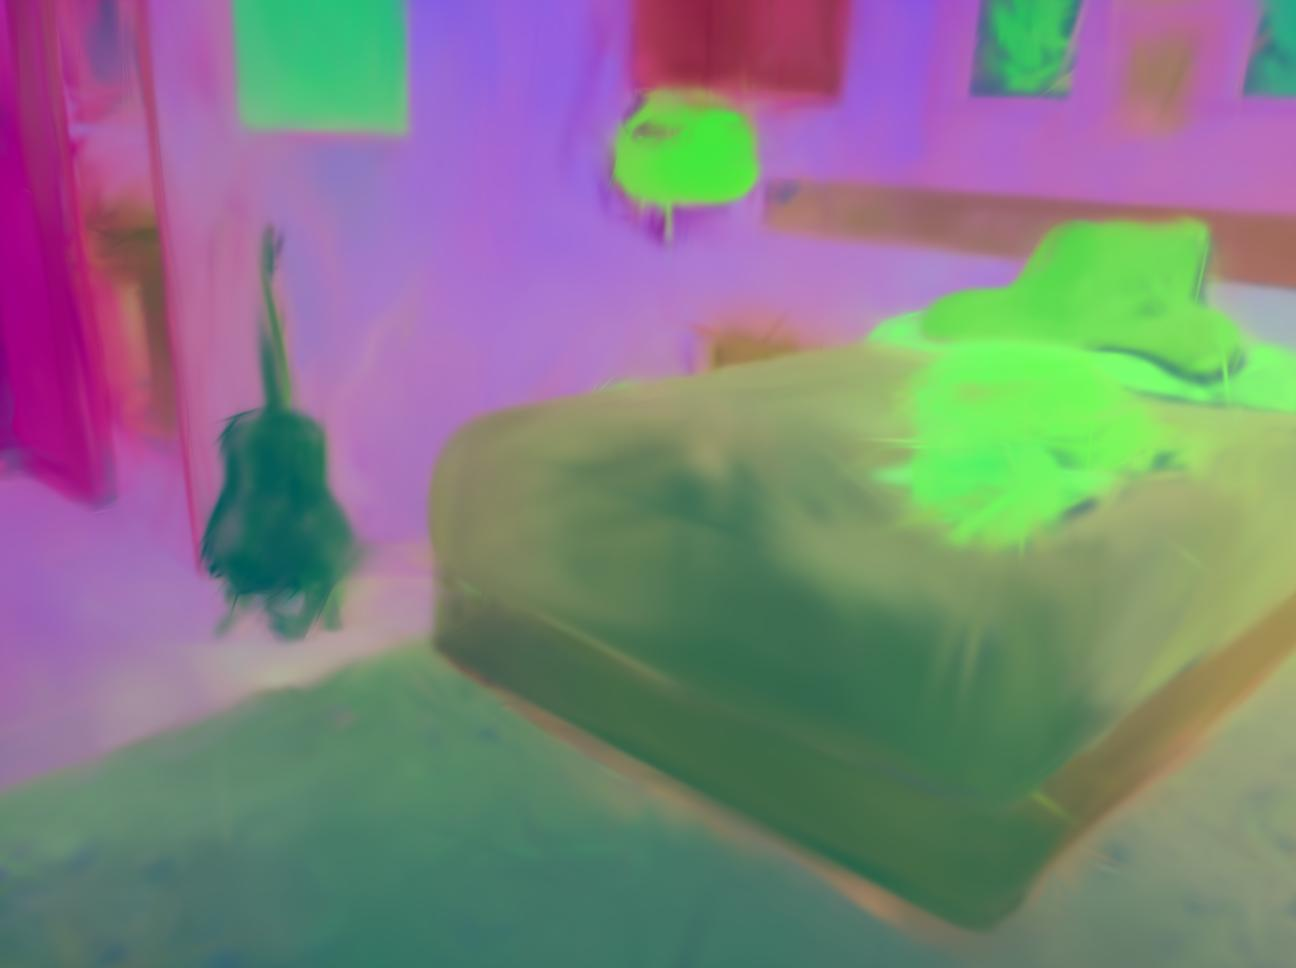
\includegraphics[width=0.32\linewidth]{figures/semantic/000_034.jpg}
    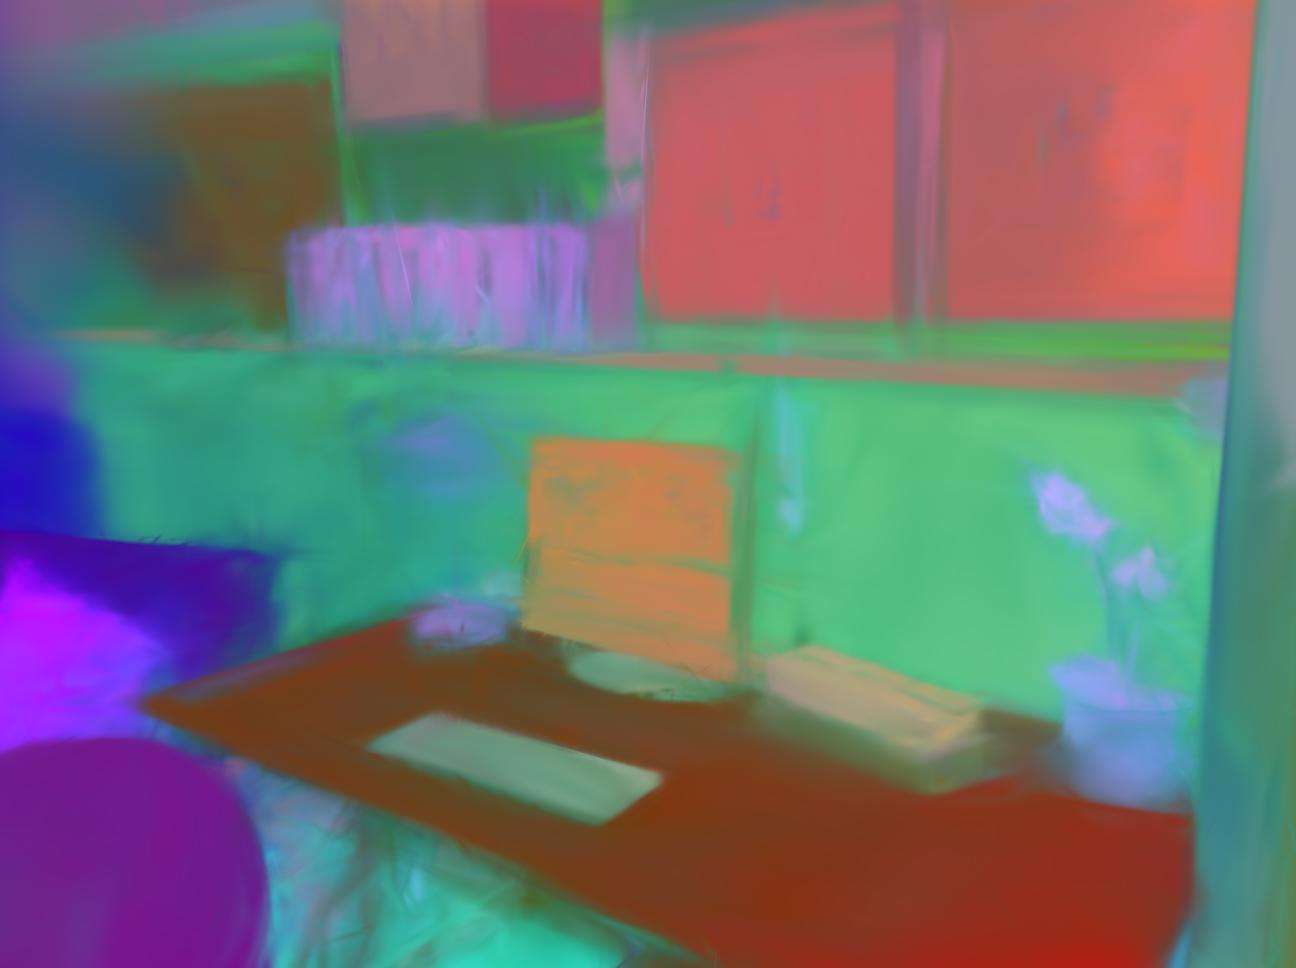
\includegraphics[width=0.32\linewidth]{figures/semantic/070_011.jpg}
    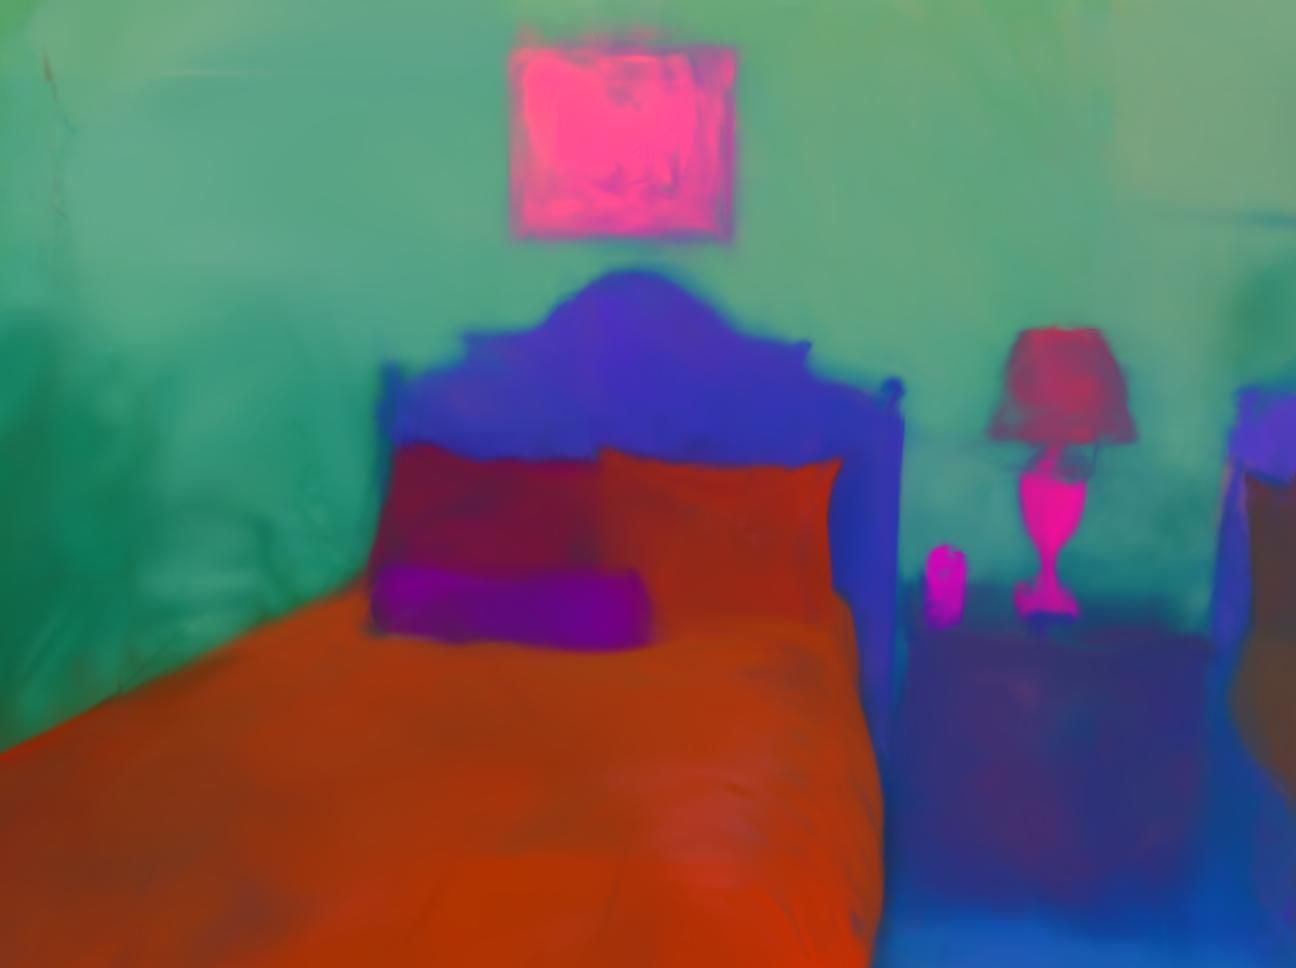
\includegraphics[width=0.32\linewidth]{figures/semantic/645_140.jpg}
    \caption{PCA of uplifted semantic features on ScanNetv2, obtained by assigning object-level CLIP features to SAM segments.}
    \label{fig:appendix-semantic}
\end{figure*}

\subsection{Comparison to GaussianEditor's uplifting}
\label{sec:appendx-gaussianeditor}

Our aggregation procedure in Eq. (\ref{eq:uplifting}) from the main paper, illustrated in Fig.~\ref{fig:uplift_render}, 
bears similarity with the one from \cite{chen2024gaussianeditor} for uplifting 2D binary masks to a 3D Gaussian splatting scene. 
In their method, uplifted masks are thresholded to create 3D binary masks that are used for semantic tracing. Specifically, they rely on rough 3D segmentation masks to selectively optimize Gaussians that are relevant for an editing task. 
Unlike in Eq.~(\ref{eq:uplifting}) and (\ref{eq:uplifting_matrix}) from the main paper,
\cite{chen2024gaussianeditor} propose to normalize their uplifted masks based on the total count of view/pixel pairs $(d,p)$ contributing to the mask of a Gaussian $i$, i.e. $\sum_{d,p\in \mathcal{S}_i} 1$, without taking the rendering weight $w_i(d,p)$ into account. Consequently, the uplifted features tend to have larger values for large, opaque Gaussians.
Fig.~\ref{fig:appendix-gaussian-editor} shows a qualitative comparison between 3D DINOv2 features obtained using the aggregation proposed by \cite{chen2024gaussianeditor} and our approach. The aggregation by \cite{chen2024gaussianeditor} fails to assign the right semantics to large gaussians, which is particularly visible in scenes with high specularity such as Room. This showcases the importance of defining 3D features as \emph{convex combinations} of 2D pixel features.

\begin{figure*}[t!]
    \centering
    \begin{subfigure}{.24\linewidth}
        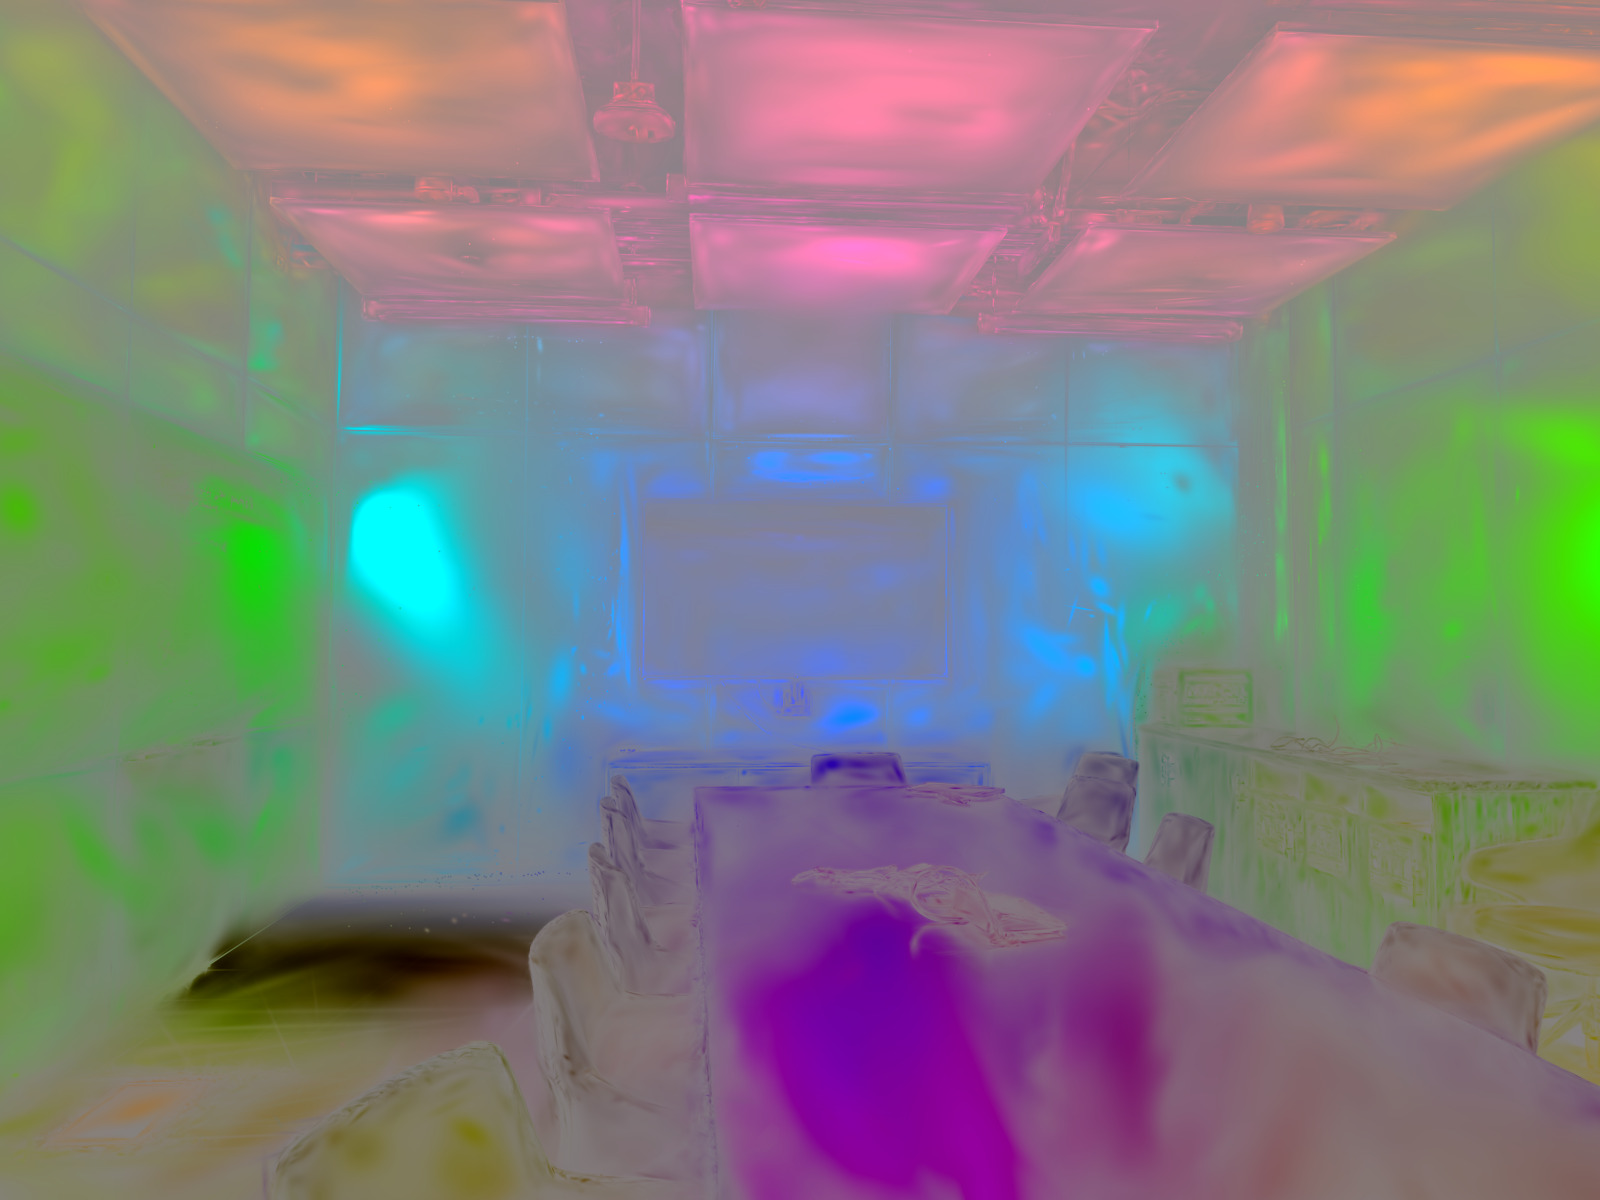
\includegraphics[width=\linewidth]{figures/gaussianeditor/room_ge.jpg}
        \caption{GaussianEditor}
    \end{subfigure}
    \begin{subfigure}{.24\linewidth}
        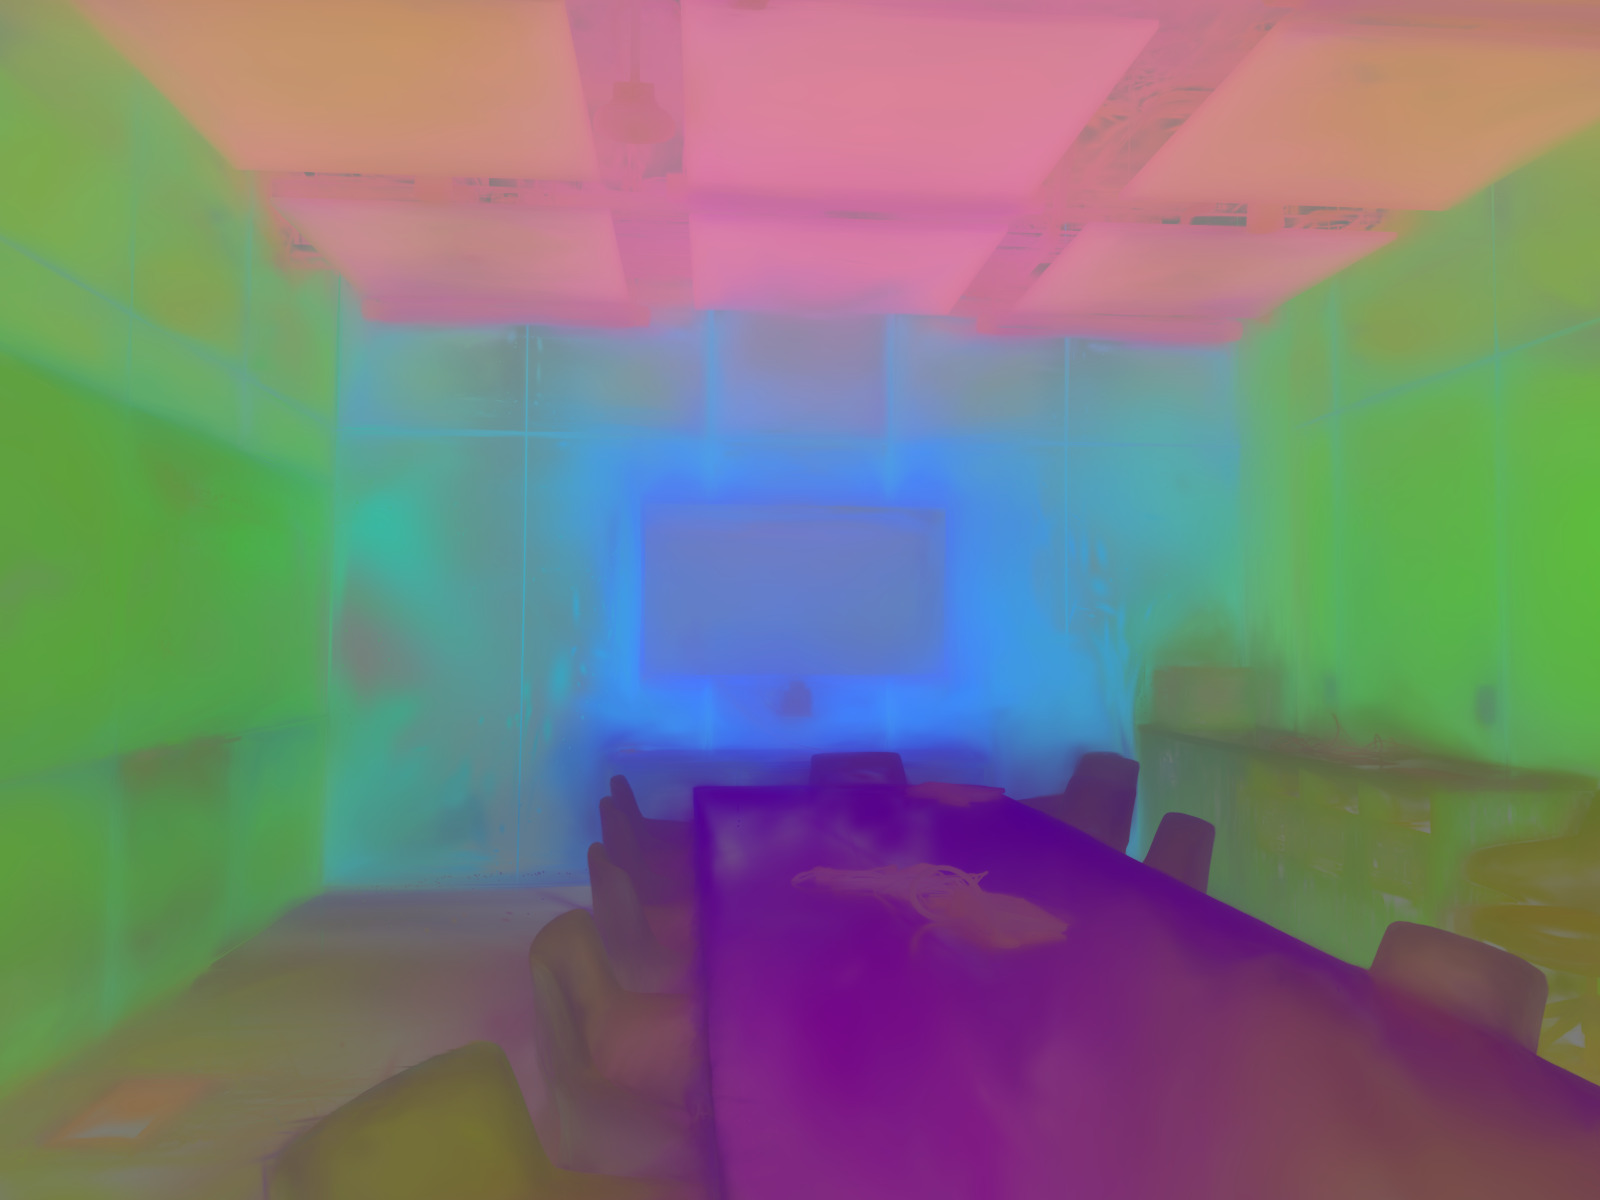
\includegraphics[width=\linewidth]{figures/gaussianeditor/room_ludvig.jpg}
        \caption{LUDVIG}
    \end{subfigure}
    \begin{subfigure}{.24\linewidth}
        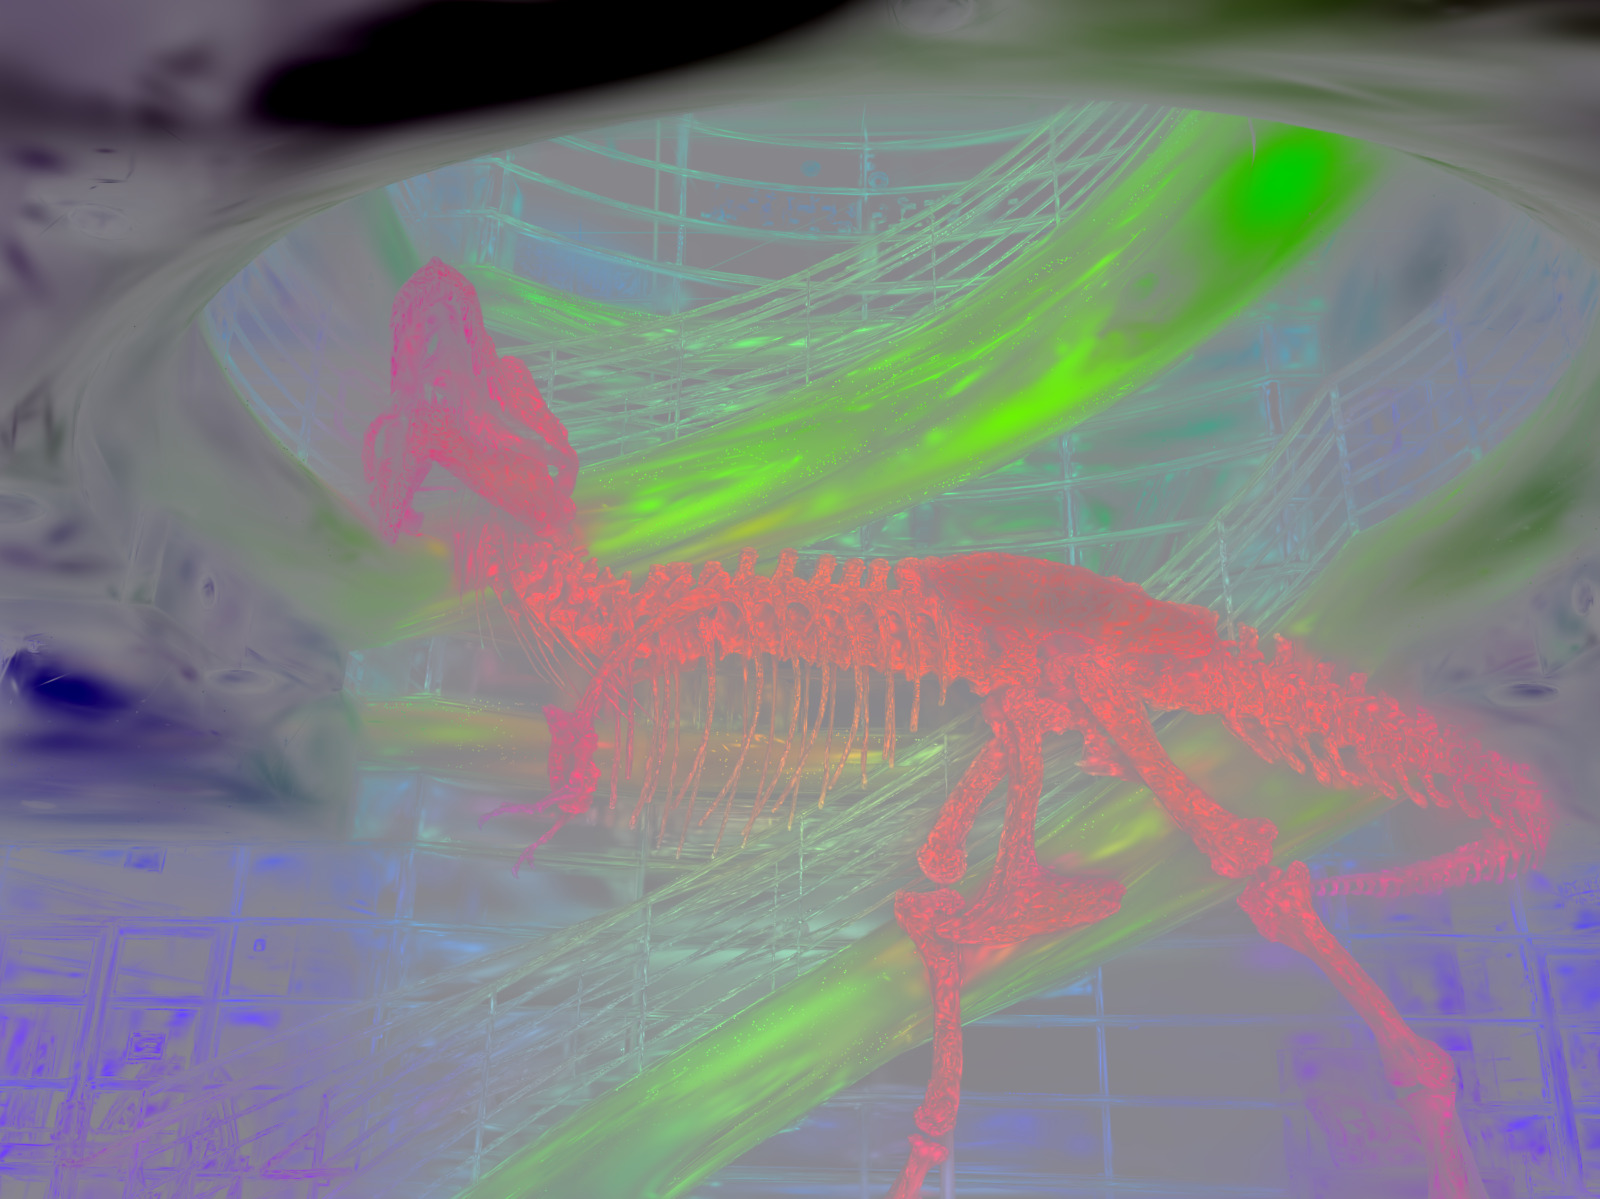
\includegraphics[width=\linewidth]{figures/gaussianeditor/trex_ge.jpg}
        \caption{GaussianEditor}
    \end{subfigure}
    \begin{subfigure}{.24\linewidth}
        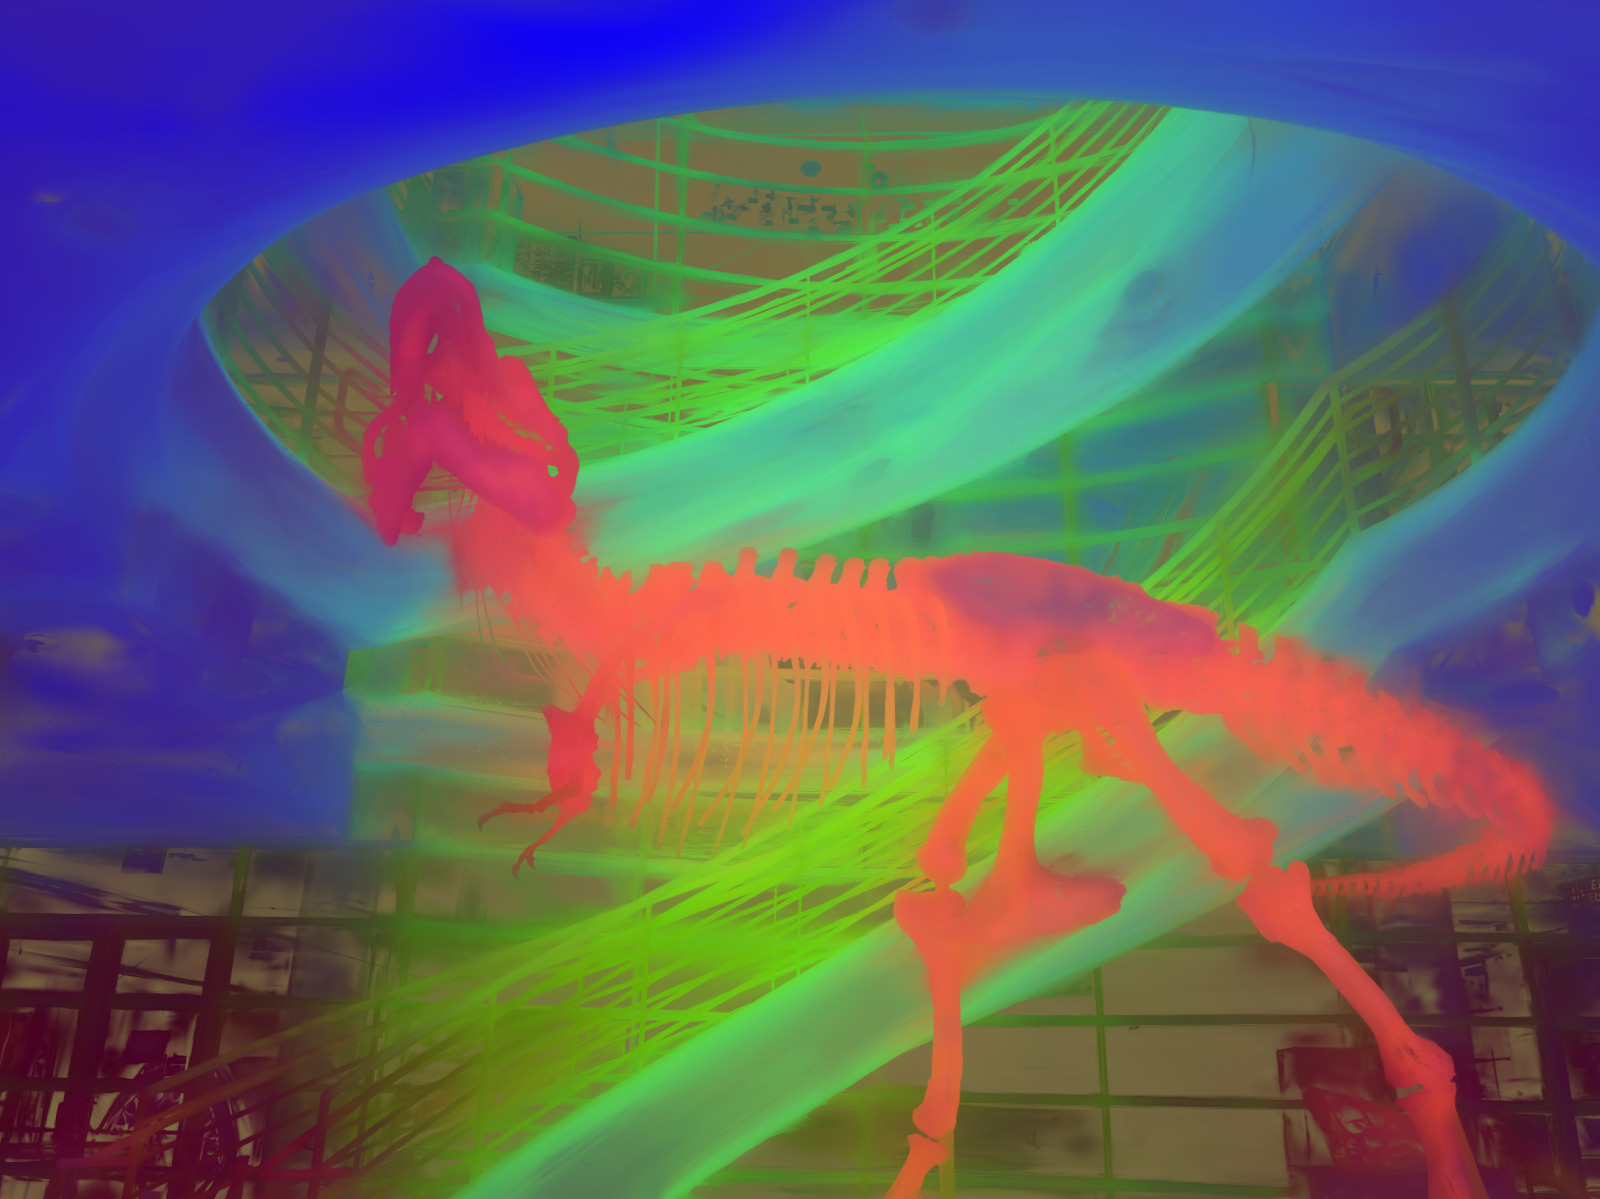
\includegraphics[width=\linewidth]{figures/pcas/trex_pca.jpg}
        \caption{LUDVIG}
    \end{subfigure}
    \caption{\textbf{Comparison to GaussianEditors's %~\citep{chen2024gaussianeditor} 
    uplifting.} Comparison of PCA visualization of uplifted features between LUDVIG's and GaussianEditor's aggregation~\citep{chen2024gaussianeditor}.}
    \label{fig:appendix-gaussian-editor}
\end{figure*}

\subsection{Visualization of CLIP segmentation results}
\label{sec:appendx-clip-visualization}

In this section, we present illustrations of the impact of the diffusion process (Fig.~\ref{fig:appendix-ablation-relevancy}), and comparative visualizations of localization heatmaps with LangSplat and LERF (Fig.~\ref{fig:appendix-clip-heatmaps}).

\subsubsection{DINOv2-guided graph diffusion}

Fig.~\ref{fig:appendix-ablation-relevancy} shows 2D segmentation masks colored by CLIP relevancy scores, obtained with and without leveraging SAM and/or DINOv2-guided graph diffusion for refining 3D relevancy scores. 

\myparagraph{Direct segmentation from raw 3D relevancy scores} Isolating a specific object in the scene directly based on CLIP relevancy scores is challenging: the segmentation masks obtained by automatic thresholding include parts of other objects with similar features, like for the \emph{sheep} (segmentation of the bear nose) and the \emph{spoon}. The segmentation might also cover surroundings of the object of interest simply due to the low resolution of CLIP visual features, such as in the \emph{knife} example. 

\myparagraph{2D segmentation with SAM} SAM delivers a precise 2D segmentation of the object covered by points with the highest relevancy scores. However, point prompts may not span the entire object, resulting in undersegmentation, like for the \emph{sheep}. In some cases, point prompts with the highest relevancy may even be located on the wrong object, resulting in an entirely wrong segmentation (\emph{e.g.}, the bowl segmented instead of the \emph{spoon}).

\myparagraph{Relevancy score refinement with graph diffusion based on 3D DINOv2 features} The graph diffusion process starts with positive weights for Gaussians with the highest relevancy scores, and propagates their weight to neighbors with similar DINOv2 features. However in cases where the object of interest consists of multiple subparts (e.g. for the \emph{sheep}), the final distribution of weights may be inhomogeneous and the automatic thresholding may select only one subpart. Also, if multiple close objects are to be segmented (e.g. with the \emph{knife}), the final weights may cover surrounding Gaussians and the final thresholding might not clearly isolate the objects.

\myparagraph{3D graph diffusion with 2D SAM segmentation}
Combining 3D graph diffusion and 2D SAM segmentation helps solving the aforementioned problems observed when using either of the two approaches individually. The diffusion process allows selecting a large set of point prompts for SAM spanning the object of interest without covering other object with similar features, resulting in an accurate segmentation.

\subsubsection{Comparisons for open-vocabulary localization} Fig.~\ref{fig:appendix-clip-heatmaps} illustrates open-vocabulary object localization with LERF~\citep{kerr2023lerf}, LangSplat~\citep{qin2023langsplat} and LUDVIG. Both LangSplat and LUDVIG correctly localize all four example objects. For queries such as the chopsticks, LangSplat's localization is more precise, as the CLIP features are constructed by generating full image segmentation masks with SAM. This process is computationally expensive, as constructing a full segmentation mask requires querying SAM over a grid of points on the image and takes about 23s for a single image (on a GPU RTX 6000 ADA), which amounts to an average of 80 minutes for a scene from the LERF dataset. However, it yields coherent instance-level CLIP representations, which is desirable for downstream segmentation tasks.

\newcommand{\plotclip}[2]{%
  \begin{tikzpicture}

    \begin{scope}[on background layer]
      \fill[blue!40, rounded corners, opacity=.5] (-1.5*#2, -1.4*#2) rectangle (1.5*#2, -.5*#2);
      \node[anchor=north east, blue!80] at (1.1*#2, -0.7*#2) {\scriptsize Graph diffusion};

      \fill[green!40, rounded corners, opacity=.5] (0.5*#2, -1.4*#2) rectangle (1.5*#2, .4*#2);
      \node[anchor=north west, green!80] at (0.8*#2, 0.2*#2) {\scriptsize SAM};
    \end{scope}
    
    % Place images with labels
    \node[anchor=center] at (-2.03*#2, 0) {\includegraphics[width=3cm]{#1_rgb.jpg}};
    \node[below=12mm] at (-2.03*#2, 0) {\scriptsize RGB image};

    \node[anchor=center] at (-2.03*#2, -.9*#2) {\includegraphics[width=3cm]{#1_gt.jpg}};
    \node[below=12mm] at (-2.03*#2, -.9*#2) {\scriptsize Ground truth};

    \node[anchor=center] at (0, 0) {\includegraphics[width=3cm]{#1_clip.jpg}};
    \node[below=12mm] at (0, 0) {\scriptsize CLIP features};

    \node[anchor=center] at (0, -.9*#2) {\includegraphics[width=3cm]{#1_dino.jpg}};
    \node[below=12mm] at (0, -.9*#2) {\scriptsize DINOv2 features};

    \node[anchor=center] at (-#2, 0) {\includegraphics[width=3cm]{#1.jpg}};
    \node[below=12mm] at (-#2, 0) {\scriptsize No diffusion, no SAM};

    \node[anchor=center] at (-#2, -.9*#2) {\includegraphics[width=3cm]{#1_dif.jpg}};
    \node[below=12mm] at (-#2, -.9*#2) {\scriptsize Diffusion, no SAM};

    \node[anchor=center] at (#2, 0) {\includegraphics[width=3cm]{#1_sam.jpg}};
    \node[below=12mm] at (#2, 0) {\scriptsize No diffusion, SAM};

    \node[anchor=center] at (#2, -.9*#2) {\includegraphics[width=3cm]{#1_dif_sam.jpg}};
    \node[below=12mm] at (#2, -.9*#2) {\scriptsize Diffusion, SAM};

    % Draw arrows
    \draw[->,line width=.7mm] (-.45*#2, 0) -- (-.55*#2, 0);
    \draw[->,line width=.7mm] (-.45*#2, -.35*#2) -- (-.55*#2, -.55*#2);
    \draw[->,line width=.7mm] (.45*#2, 0) -- (.55*#2, 0);
    \draw[->,line width=.7mm] (.45*#2, -.35*#2) -- (.55*#2, -.55*#2);
    \draw[->,line width=.7mm] (-.45*#2, -.9*#2) -- (-.55*#2, -.9*#2);
    \draw[->,line width=.7mm] (.45*#2, -.9*#2) -- (.55*#2, -.9*#2);

  \end{tikzpicture}%
}
\begin{figure*}
    \centering
    \plotclip{figures/ablation_relevancy/spoon}{3.5} \\ \vspace{.5cm}
    \plotclip{figures/ablation_relevancy/knife}{3.5} \\ \vspace{.5cm}
    \plotclip{figures/ablation_relevancy/sheep}{3.5}
    \caption{\textbf{Open-vocabulary object segmentation with and without using 3D graph diffusion (blue) and/or 2D SAM segmentation (green).} Projections of 3D CLIP and DINOv2 features colored by three main PCA components and 2D segmentation masks colored by relevancy scores.}
    \label{fig:appendix-ablation-relevancy}
\end{figure*}


\begin{figure*}
    \centering
    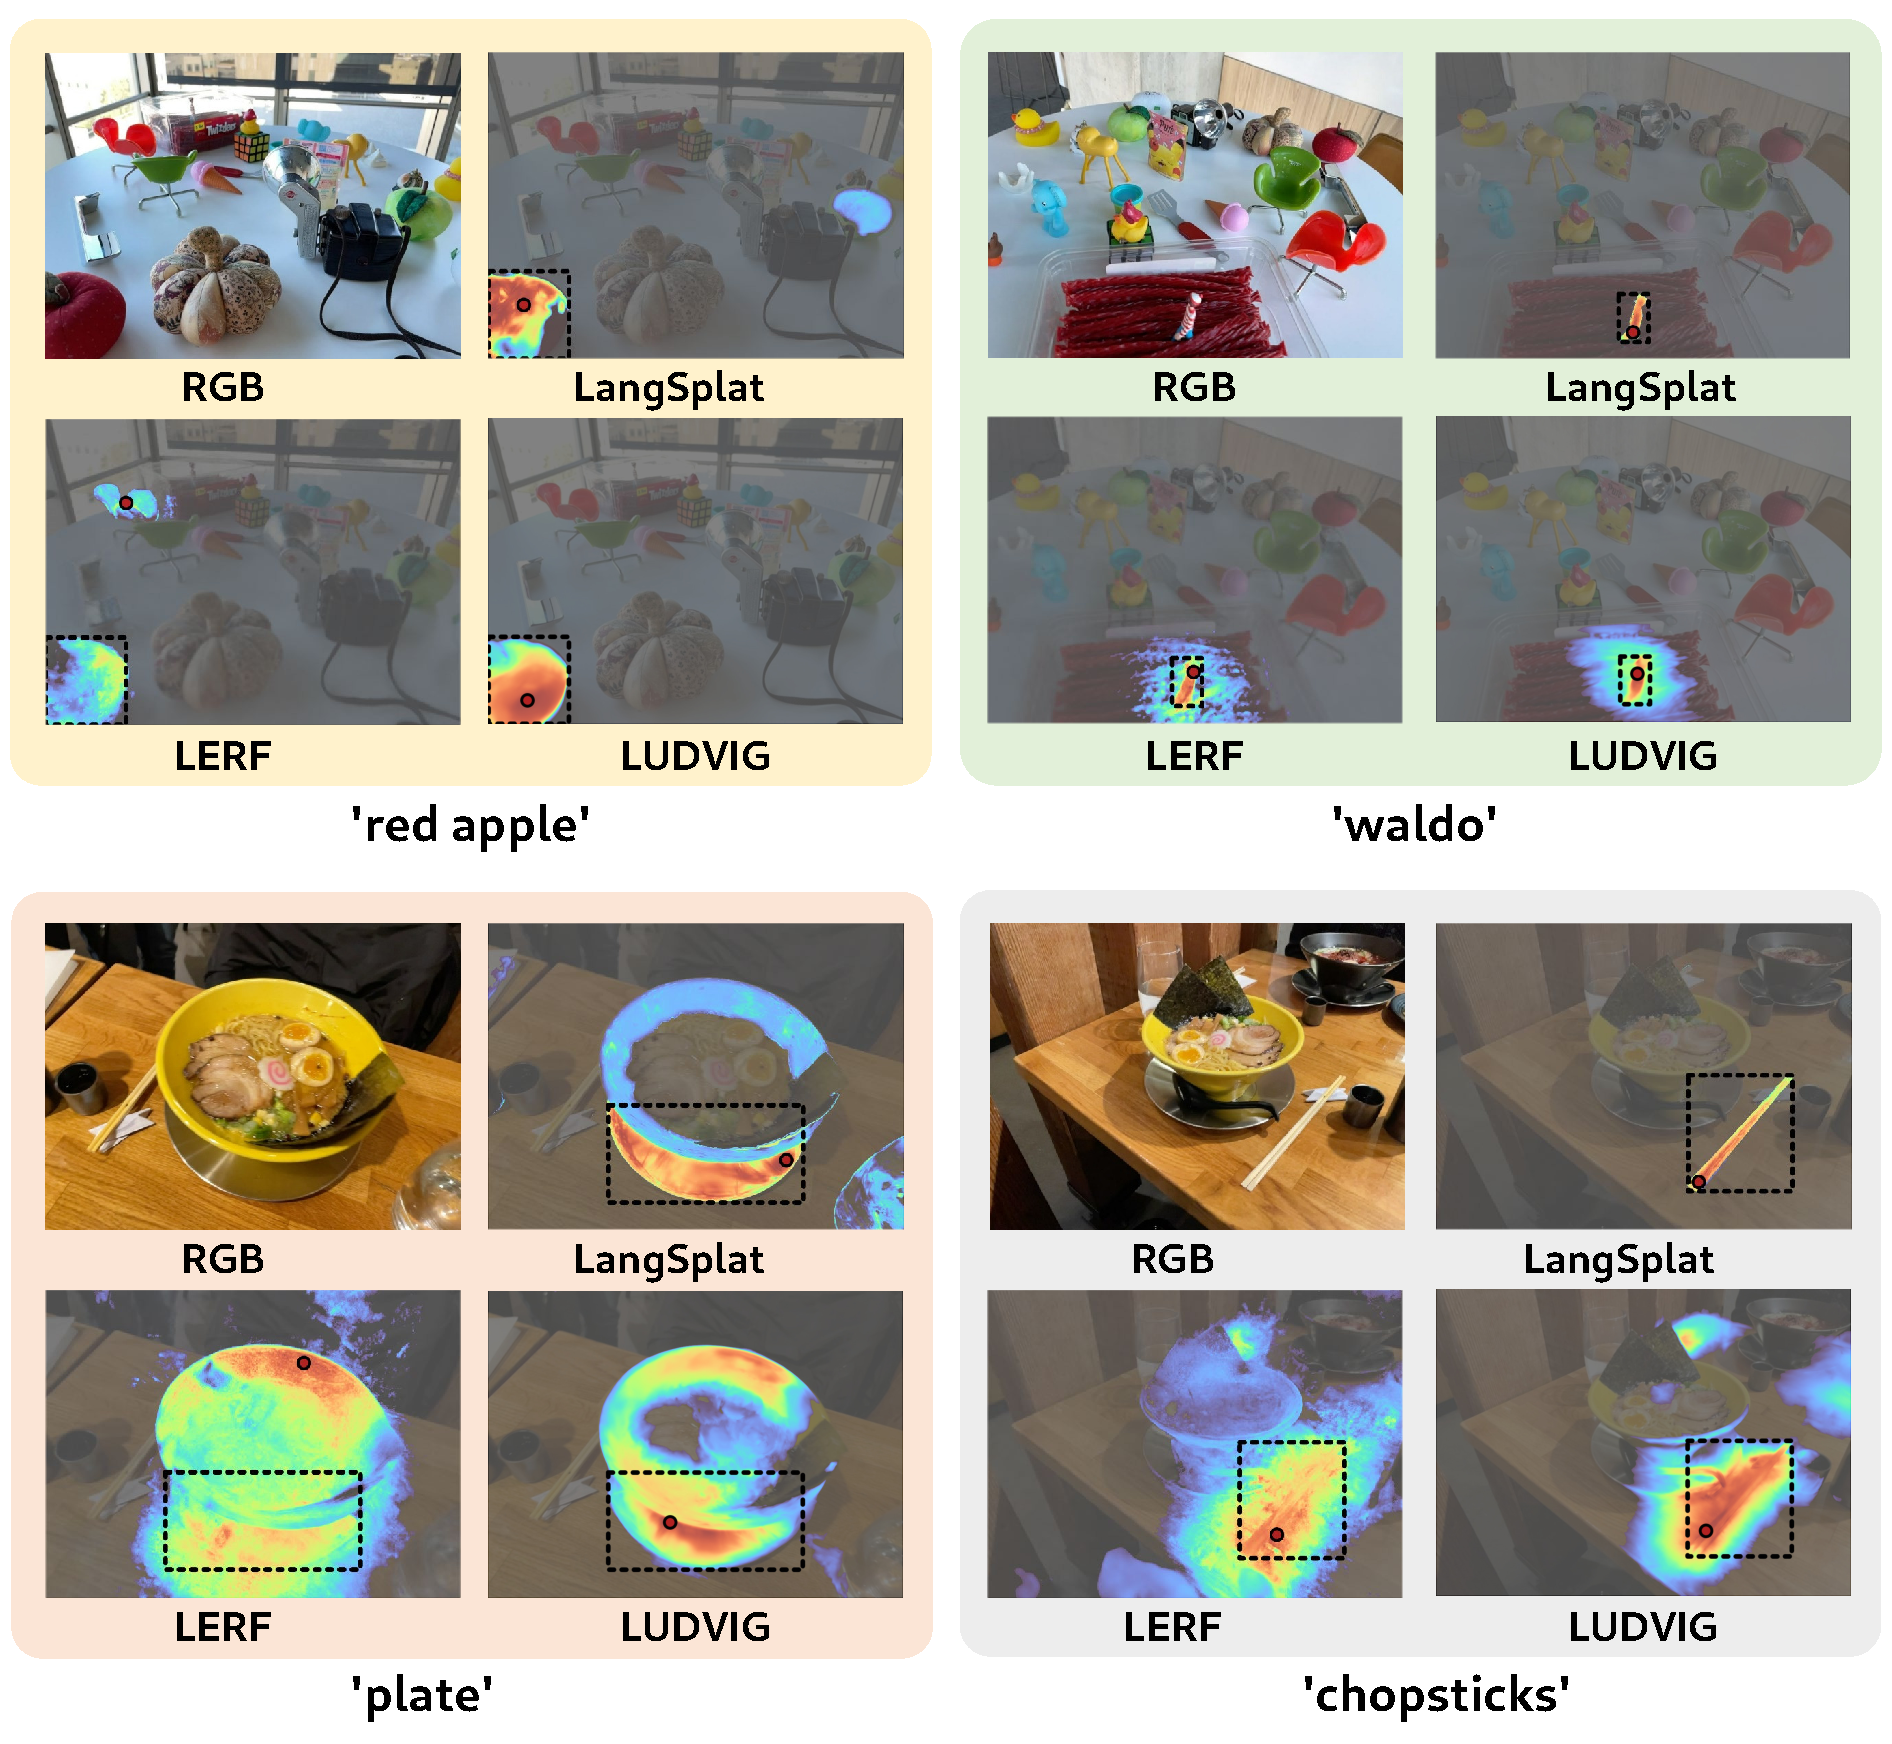
\includegraphics[width=\linewidth]{figures/localization_heatmaps.pdf}
    \caption{\textbf{Qualitative comparisons of open-vocabulary 3D object localization on the LERF dataset.} The red points are the model predictions and the black dashed bounding boxes denote the annotations. This figure is taken and adapted from LangSplat's website (https://langsplat.github.io/), licensed under a Creative Commons Attribution-ShareAlike 4.0 International License.}
    \label{fig:appendix-clip-heatmaps}
\end{figure*}
